% Options for packages loaded elsewhere
\PassOptionsToPackage{unicode}{hyperref}
\PassOptionsToPackage{hyphens}{url}
%
\documentclass[
  14pt,
]{book}
\usepackage{lmodern}
\usepackage{amssymb,amsmath}
\usepackage{ifxetex,ifluatex}
\ifnum 0\ifxetex 1\fi\ifluatex 1\fi=0 % if pdftex
  \usepackage[T1]{fontenc}
  \usepackage[utf8]{inputenc}
  \usepackage{textcomp} % provide euro and other symbols
\else % if luatex or xetex
  \usepackage{unicode-math}
  \defaultfontfeatures{Scale=MatchLowercase}
  \defaultfontfeatures[\rmfamily]{Ligatures=TeX,Scale=1}
\fi
% Use upquote if available, for straight quotes in verbatim environments
\IfFileExists{upquote.sty}{\usepackage{upquote}}{}
\IfFileExists{microtype.sty}{% use microtype if available
  \usepackage[]{microtype}
  \UseMicrotypeSet[protrusion]{basicmath} % disable protrusion for tt fonts
}{}
\makeatletter
\@ifundefined{KOMAClassName}{% if non-KOMA class
  \IfFileExists{parskip.sty}{%
    \usepackage{parskip}
  }{% else
    \setlength{\parindent}{0pt}
    \setlength{\parskip}{6pt plus 2pt minus 1pt}}
}{% if KOMA class
  \KOMAoptions{parskip=half}}
\makeatother
\usepackage{xcolor}
\IfFileExists{xurl.sty}{\usepackage{xurl}}{} % add URL line breaks if available
\IfFileExists{bookmark.sty}{\usepackage{bookmark}}{\usepackage{hyperref}}
\hypersetup{
  pdftitle={Panel Ciudadanía Escolar},
  hidelinks,
  pdfcreator={LaTeX via pandoc}}
\urlstyle{same} % disable monospaced font for URLs
\usepackage{longtable,booktabs}
% Correct order of tables after \paragraph or \subparagraph
\usepackage{etoolbox}
\makeatletter
\patchcmd\longtable{\par}{\if@noskipsec\mbox{}\fi\par}{}{}
\makeatother
% Allow footnotes in longtable head/foot
\IfFileExists{footnotehyper.sty}{\usepackage{footnotehyper}}{\usepackage{footnote}}
\makesavenoteenv{longtable}
\usepackage{graphicx,grffile}
\makeatletter
\def\maxwidth{\ifdim\Gin@nat@width>\linewidth\linewidth\else\Gin@nat@width\fi}
\def\maxheight{\ifdim\Gin@nat@height>\textheight\textheight\else\Gin@nat@height\fi}
\makeatother
% Scale images if necessary, so that they will not overflow the page
% margins by default, and it is still possible to overwrite the defaults
% using explicit options in \includegraphics[width, height, ...]{}
\setkeys{Gin}{width=\maxwidth,height=\maxheight,keepaspectratio}
% Set default figure placement to htbp
\makeatletter
\def\fps@figure{htbp}
\makeatother
\setlength{\emergencystretch}{3em} % prevent overfull lines
\providecommand{\tightlist}{%
  \setlength{\itemsep}{0pt}\setlength{\parskip}{0pt}}
\setcounter{secnumdepth}{5}
\usepackage{booktabs}
\usepackage{float}
\let\origfigure\figure
\let\endorigfigure\endfigure
\renewenvironment{figure}[1][2] {
  \expandafter\origfigure\expandafter[H]
} {
  \endorigfigure
}
\usepackage[]{natbib}
\bibliographystyle{apalike}

\title{Panel Ciudadanía Escolar}
\usepackage{etoolbox}
\makeatletter
\providecommand{\subtitle}[1]{% add subtitle to \maketitle
  \apptocmd{\@title}{\par {\large #1 \par}}{}{}
}
\makeatother
\subtitle{Reporte de resultados Primera Ola 2019}
\author{}
\date{\vspace{-2.5em}2020-09-29}

\begin{document}
\maketitle

{
\setcounter{tocdepth}{1}
\tableofcontents
}
\hypertarget{introducciuxf3n}{%
\chapter*{Introducción}\label{introducciuxf3n}}
\addcontentsline{toc}{chapter}{Introducción}

El involucramiento político de las y los ciudadanas/os es un requisito fundamental de las democracias modernas, y es justamente su visible erosión lo que se diagnóstica como crisis de legitimidad y representación de las mismas. Al mismo tiempo es evidente una ampliación de los repertorios de participación política, especialmente por parte de los jóvenes. Las respuestas desde las políticas públicas a estos rasgos paradojales, en el primer mundo como en Chile, se han enfocado al sistema educativo, sin considerar suficientemente el problema de las desigualdades de origen que afectan a las capacidades de participación, ni tampoco suficientemente las capacidades de agencia que exhiben las nuevas generaciones. En este marco el presente proyecto se propone investigar la socialización política de las nuevas generaciones, o el proceso y mecanismos de adquisición de unas creencias, conocimientos, actitudes y prácticas para el ejercicio de la ciudadanía, en las dos agencias clave de socialización: la familia y la escuela. La pregunta que articula el conjunto es: \emph{¿En qué medida la escuela es un agente reproductor o mitigador de la transmisión intergeneracional de la desigualdad política familiar?} Su respuesta supone un diseño que aborde en profundidad tanto los efectos como los mecanismos de ambas agencias, desde una perspectiva evaluativa que interroga por los factores que profundizan o mitigan las desigualdades en socialización política.

Este reporte resume los principales resultados del estudio \textbf{Panel de Ciudadanía Escolar - PACES}.

Estructura del reporte:

\textbf{Diseño Metodológico}

\textbf{Módulo 1: Conocimiento y formación en la escuela}

\begin{itemize}
\tightlist
\item
  1.1 Conocimiento cívico PACES
\item
  1.2 Comparación conocimiento cívico PACES / ICCS
\item
  1.3 Buena ciudadanía
\end{itemize}

\textbf{Módulo 2: Actitudes políticas}

\begin{itemize}
\tightlist
\item
  2.1 Interés en la política y en los problemas sociales
\item
  2.2 Satisfacción con la democracia y actitudes autoritarias
\item
  2.3 Confianza en grupos e instituciones
\end{itemize}

\textbf{Módulo 3: Participación}

\begin{itemize}
\tightlist
\item
  2.1 Participación formal
\item
  2.2 Participación activista
\item
  2.3 Participación comunitaria
\end{itemize}

\hypertarget{documento-de-presentaciuxf3n-seminario-30-septiembre-2020}{%
\section*{Documento de presentación seminario 30 Septiembre 2020}\label{documento-de-presentaciuxf3n-seminario-30-septiembre-2020}}
\addcontentsline{toc}{section}{Documento de presentación seminario 30 Septiembre 2020}

\hypertarget{reporte-metodoluxf3gico}{%
\chapter*{Reporte metodológico}\label{reporte-metodoluxf3gico}}
\addcontentsline{toc}{chapter}{Reporte metodológico}

Para abordar esta pregunta se lleva a cabo un Estudio Panel de Ciudadanía Escolar entre 2019 y 2021, evaluando a una muestra representativa de padres, docentes y estudiantes de enseñanza media. A continuación se presentan un esquema que resume el diseño metodológico longitudinal del estudio.

\textbf{Diseño del Estudio Panel de Ciudadanía Escolar - PACES}

\begin{center}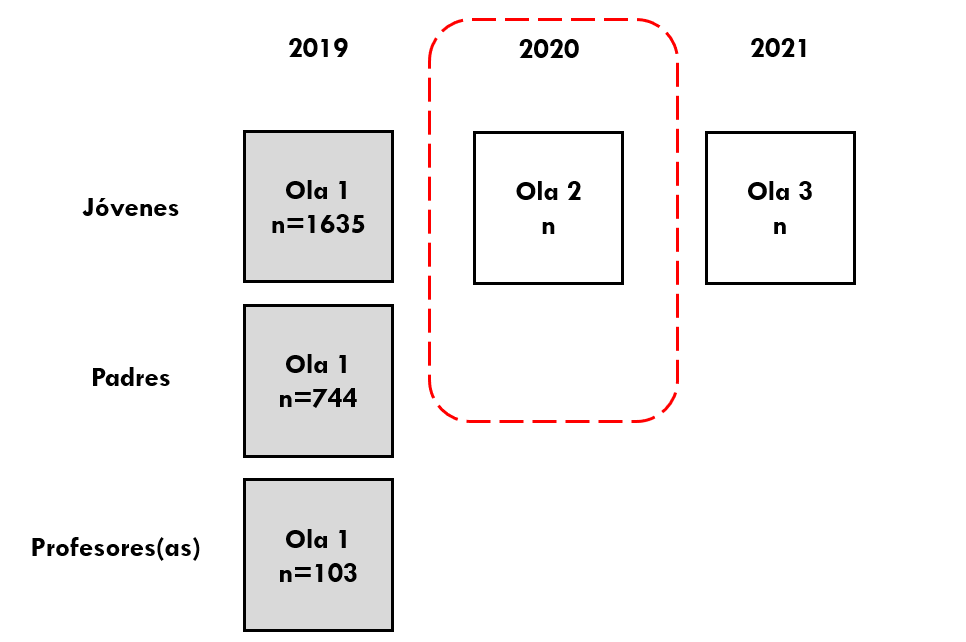
\includegraphics[width=0.8\linewidth,]{images/diseno1} \end{center}

\hypertarget{conocimiento-y-formaciuxf3n-en-la-escuela}{%
\chapter{Conocimiento y formación en la escuela}\label{conocimiento-y-formaciuxf3n-en-la-escuela}}

El reporte de los resultados correspondientes a este módulo se organiza en dos secciones. En la primera sección se presentarán las respuestas de los estudiantes a un set de preguntas que evalúan su nivel de conocimiento cívico. En la segunda sección se expondrán las respuestas de los docentes, estudiantes y apoderados a una serie de preguntas sobre el nivel de importancia de distintos aspectos en la formación ciudadana de los estudiantes y sobre quiénes son los que más influyen en la enseñanza de estos aspectos.

\hypertarget{conocimiento-cuxedvico-paces}{%
\section{Conocimiento cívico PACES}\label{conocimiento-cuxedvico-paces}}

En esta sección se presentarán los resultados de una serie de preguntas que evalúan el nivel de conocimiento de los estudiantes de segundo año de enseñanza media sobre diversos temas cívicos, políticos y sociales.

Las primeras ocho interrogantes que se presentarán en esta subsección son parte de un set de preguntas que evalúa distintas aristas del \textbf{conocimiento cívico conceptual}. Las seis preguntas restantes evalúan diferentes dimensiones del \textbf{conocimiento cívico factual}

En relación con el patrón de respuestas cabe destacar que, en general, la mayoría de los estudiantes respondió las preguntas de forma correcta (entre un 43.4\% y un 80.9\% de los encuestados) y que, en algunas preguntas, las respuestas incorrectas se concentraron en una alternativa en particular.

\begin{center}\rule{0.5\linewidth}{0.5pt}\end{center}

\begin{figure}[!ht]

{\centering 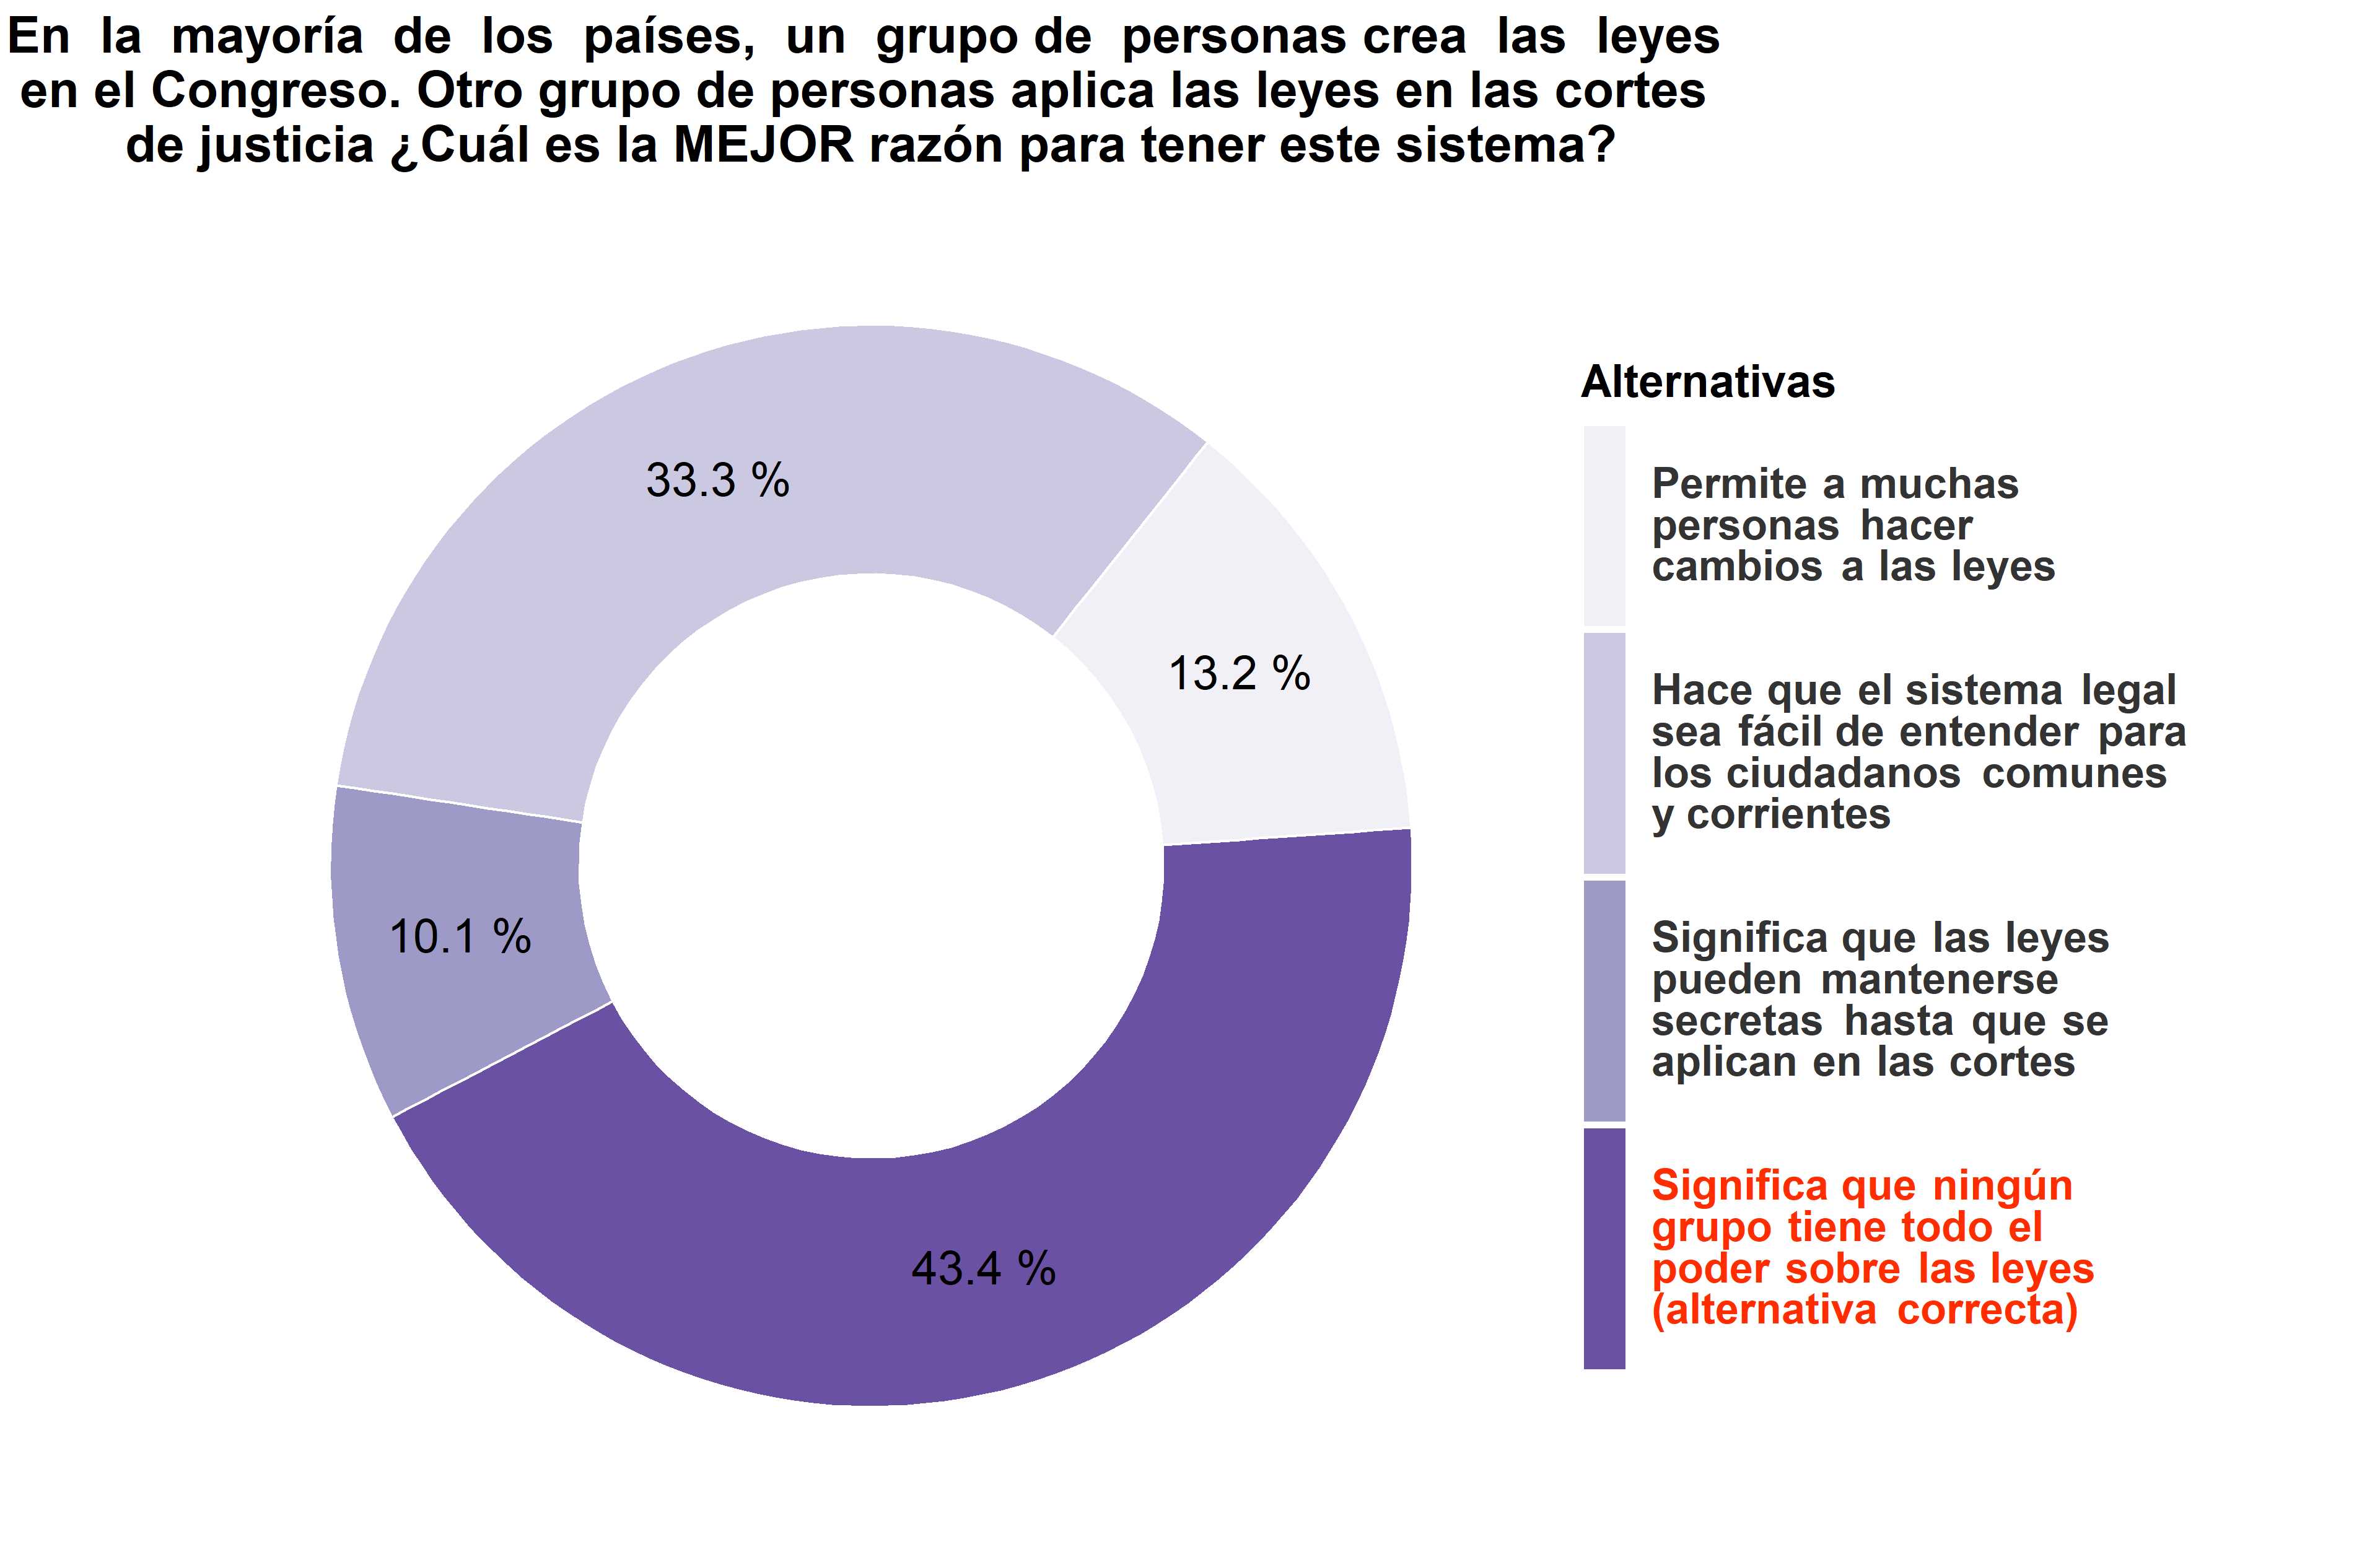
\includegraphics[width=0.8\linewidth,]{images/ccivico_1} 

}

\caption{Razones para crear leyes en el Congreso}\label{fig:unnamed-chunk-5}
\end{figure}

Un 43.4\% de los estudiantes respondió correctamente la pregunta. Entre las alternativas incorrectas, hubo una que distrajó a parte importante de los estudiantes, concentrando el 33.3\% de las respuestas.

\begin{center}\rule{0.5\linewidth}{0.5pt}\end{center}

\begin{figure}[!ht]

{\centering 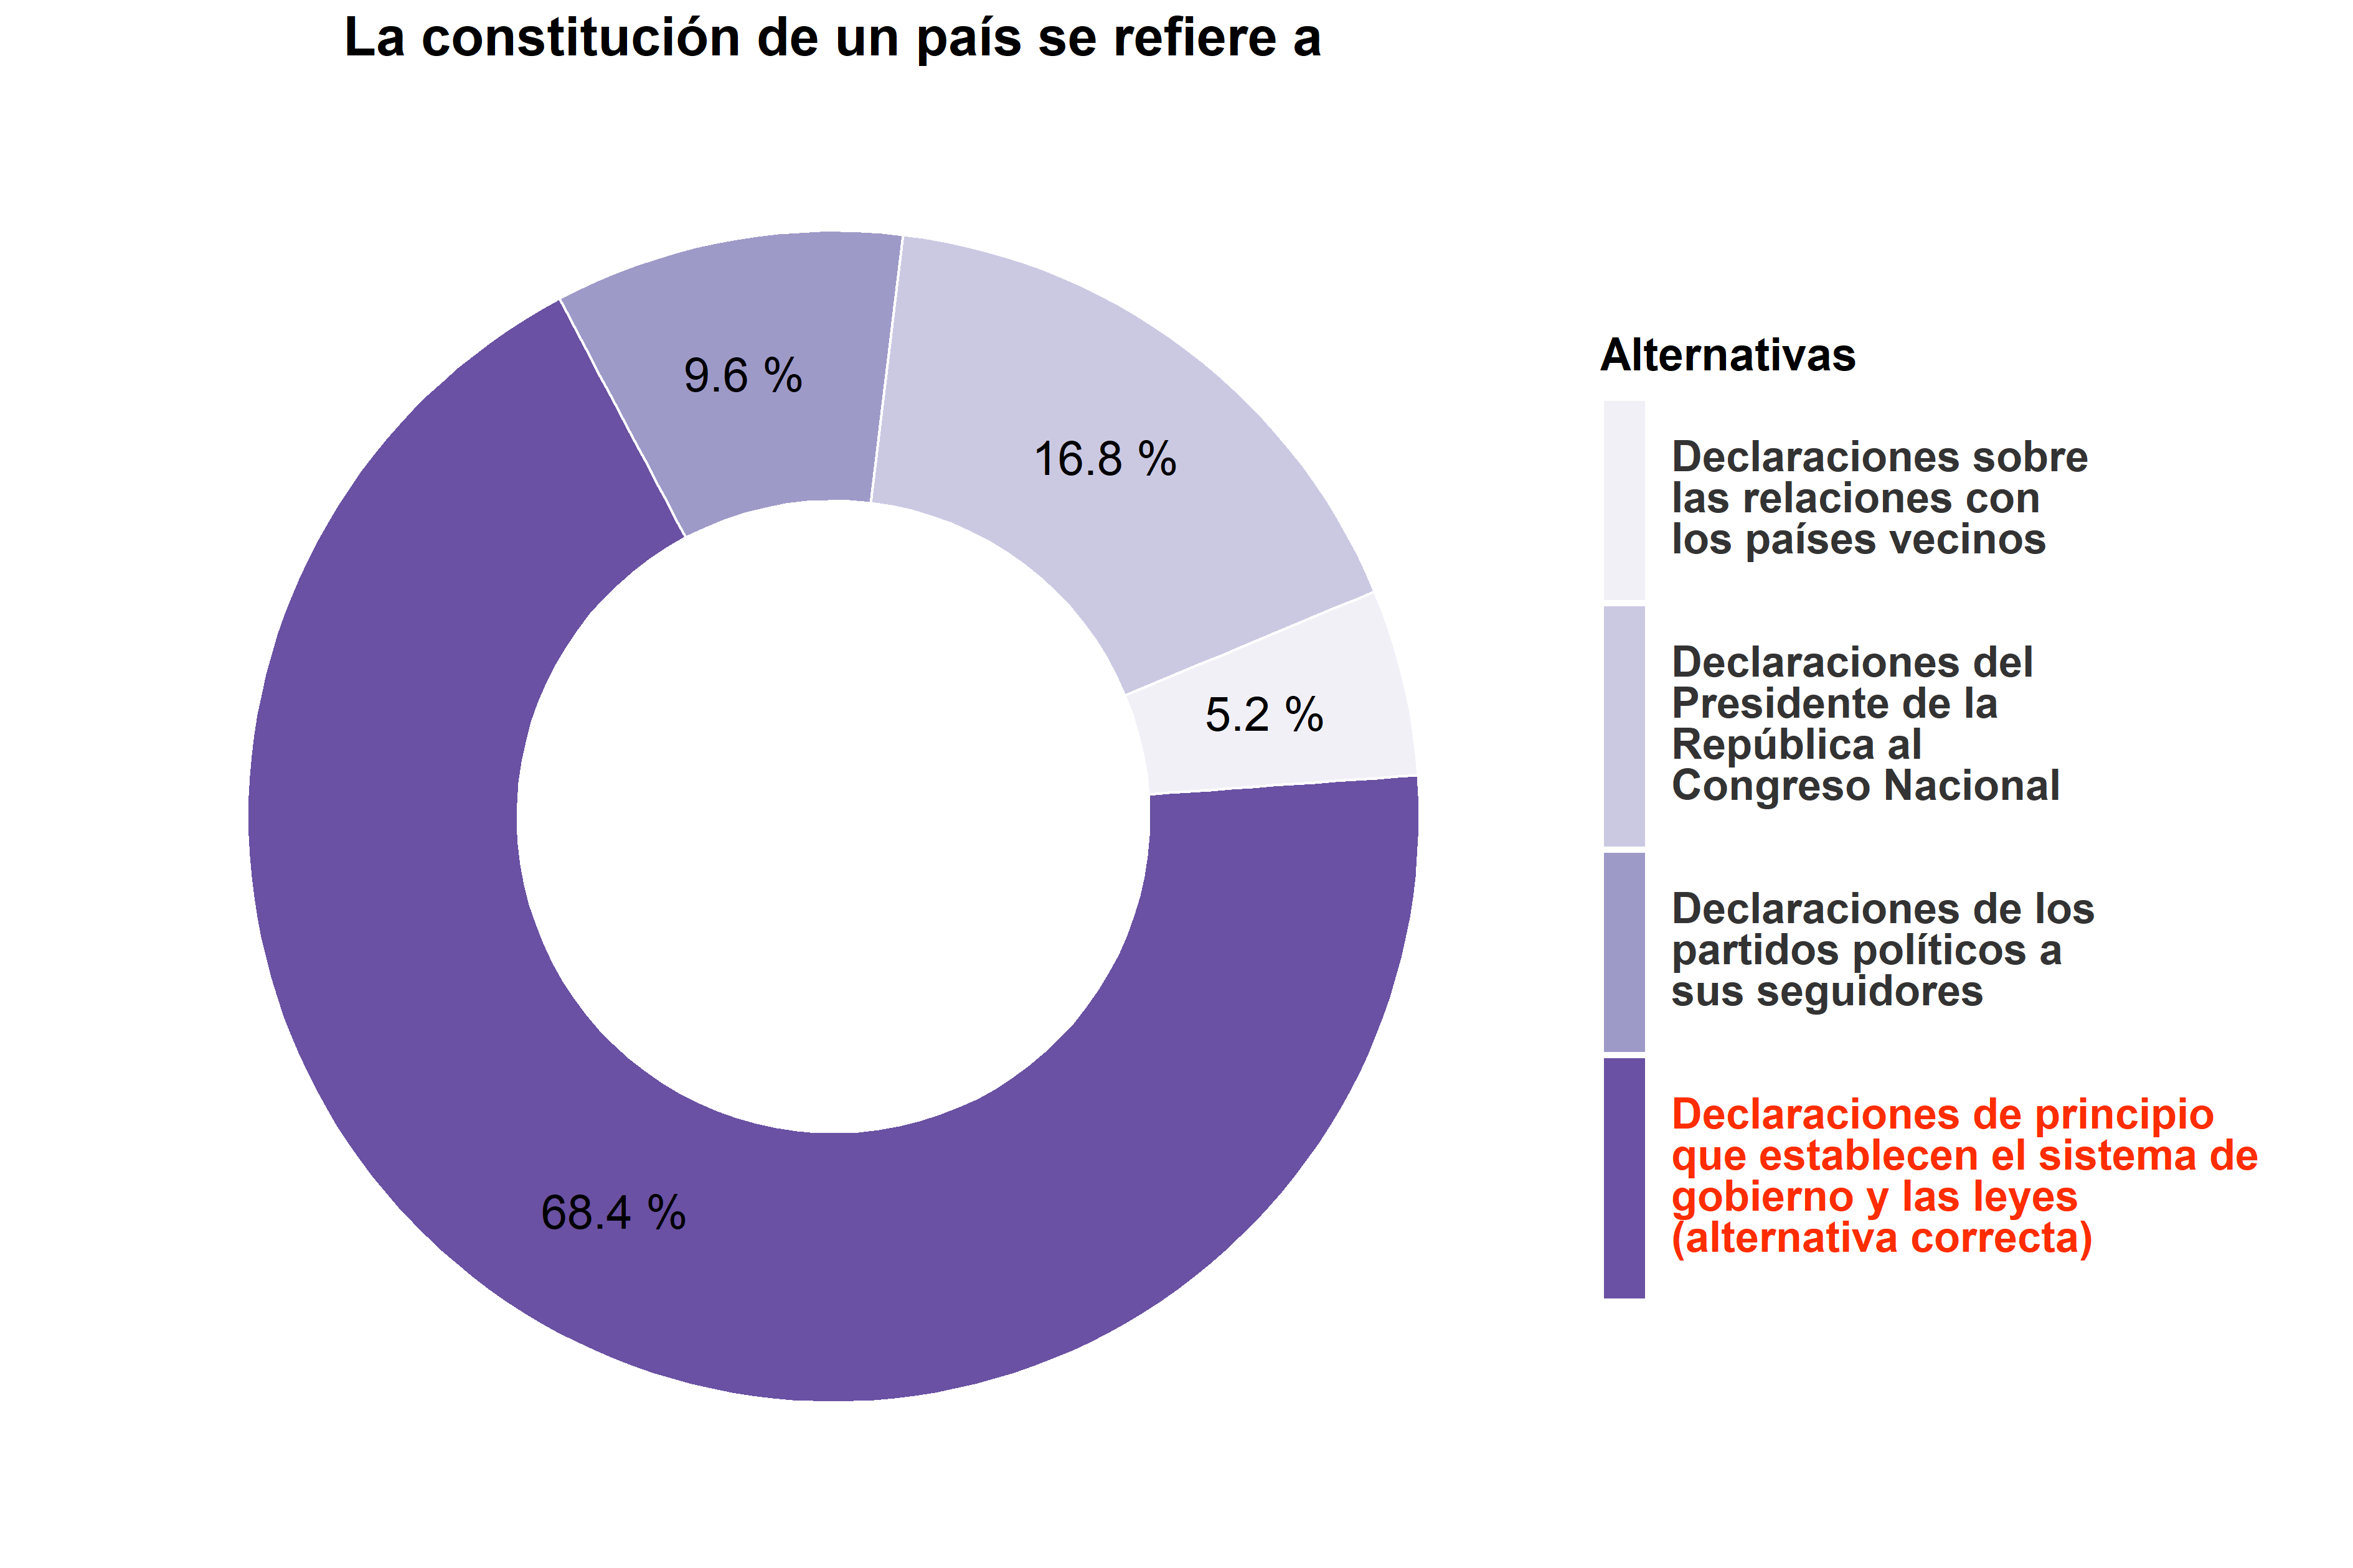
\includegraphics[width=0.8\linewidth,]{images/ccivico_2} 

}

\caption{Definiciones de constitución}\label{fig:unnamed-chunk-6}
\end{figure}

La mayoría de los estudiantes (un 70.6\%) respondió de forma correcta. Las respuestas incorrectas se concentraron en una alternativa en particular, la cual fue seleccionada por el 16\% de los encuestados.

\begin{center}\rule{0.5\linewidth}{0.5pt}\end{center}

\begin{figure}[!ht]

{\centering 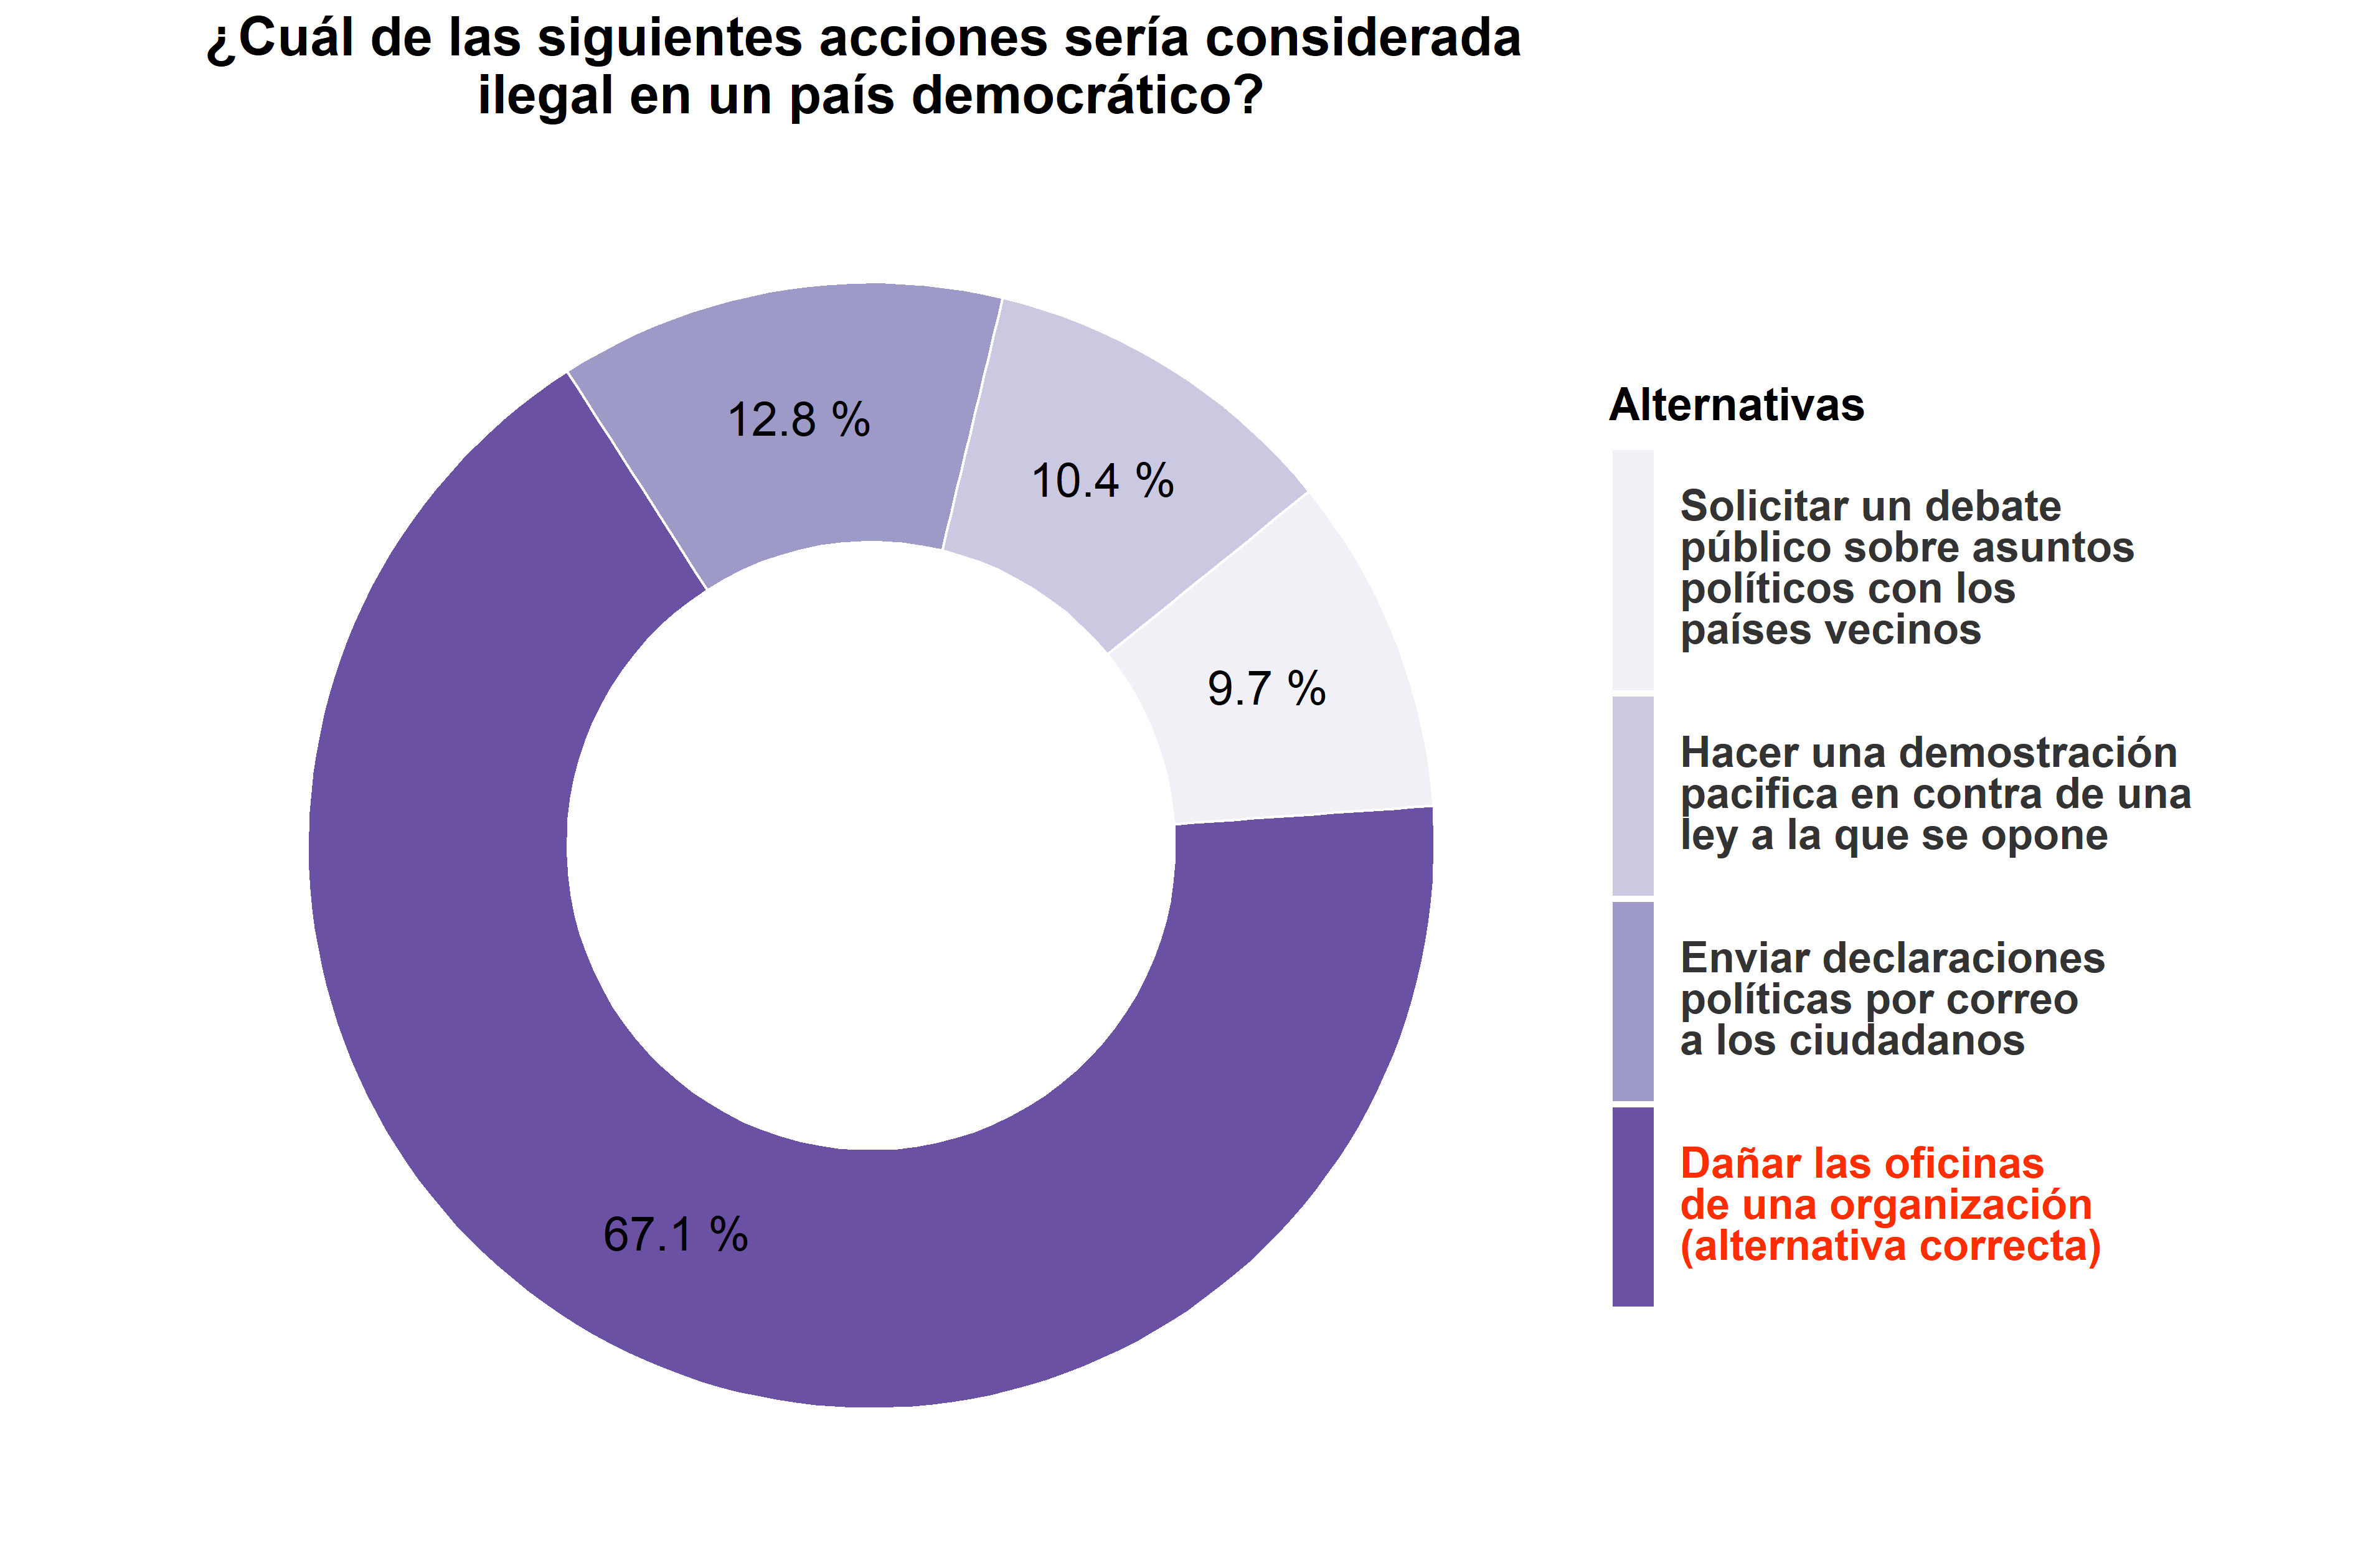
\includegraphics[width=0.8\linewidth,]{images/ccivico_3} 

}

\caption{Acción ilegal en un país democrático}\label{fig:unnamed-chunk-7}
\end{figure}

La mayoría de los estudiantes (un 69.2\%) seleccionó la alternativa correcta. Las respuestas incorrectas no se concentraron en una alternativa en particular.

\begin{center}\rule{0.5\linewidth}{0.5pt}\end{center}

\begin{figure}[!ht]

{\centering 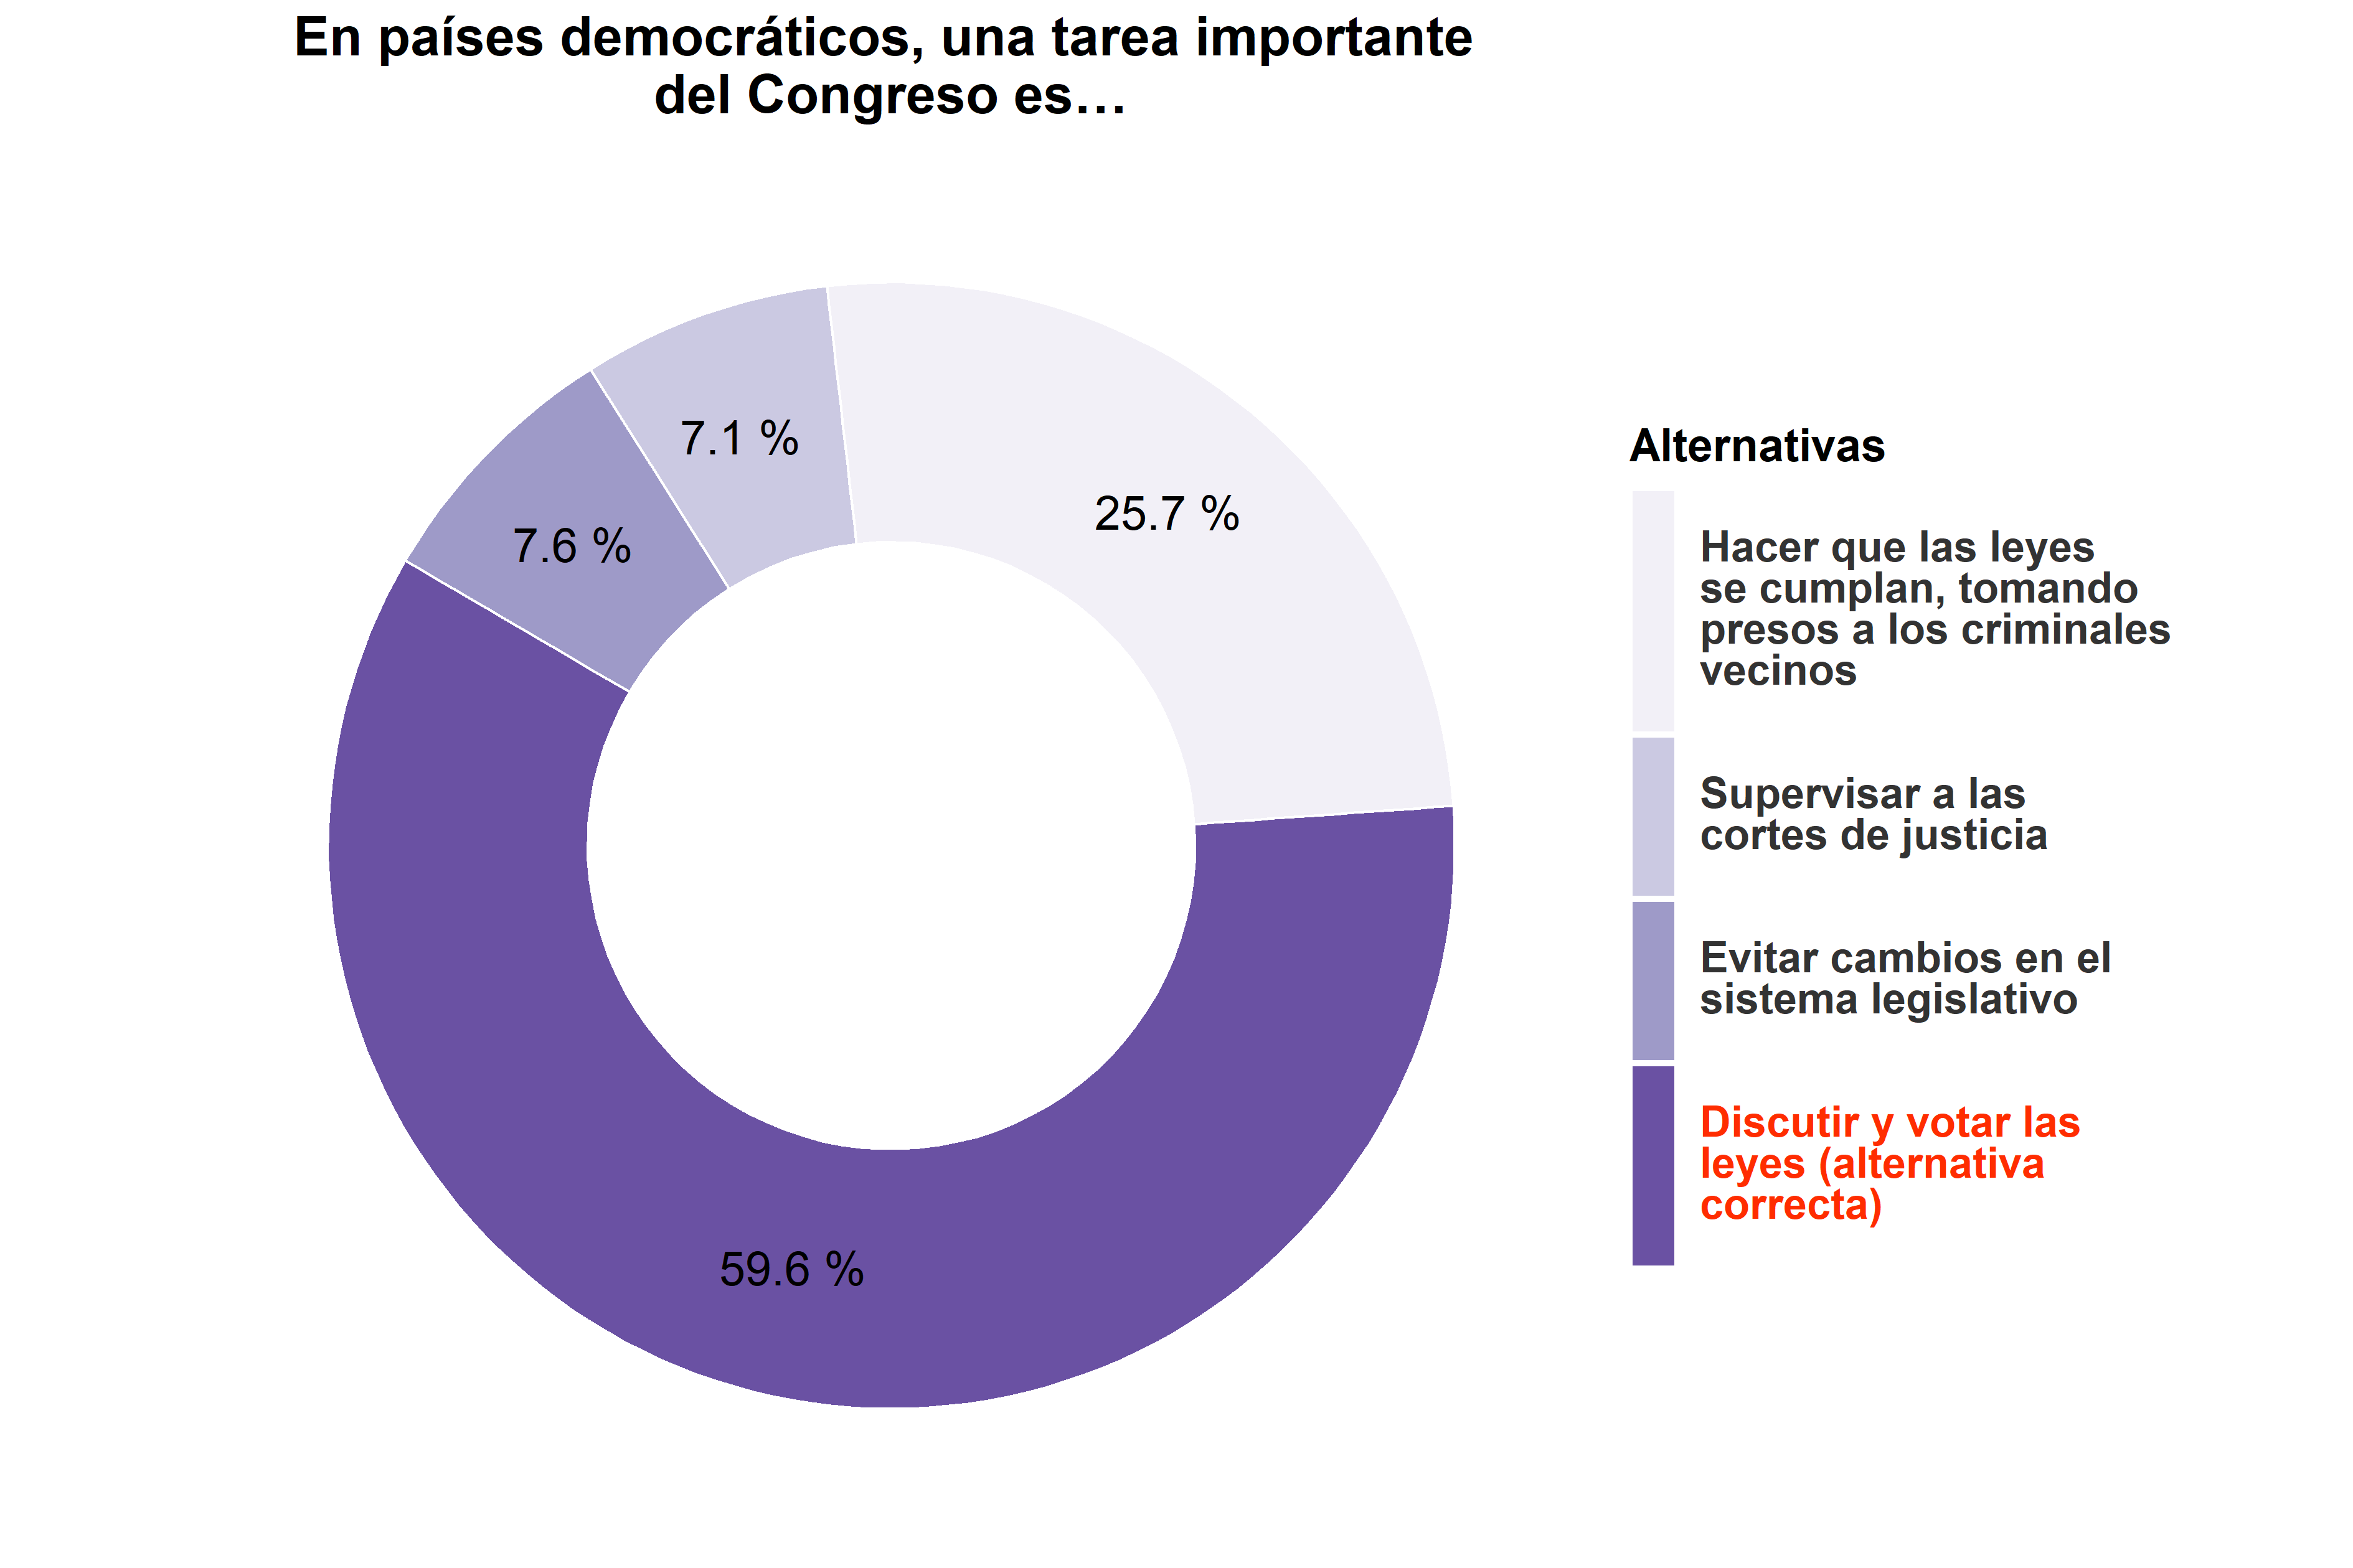
\includegraphics[width=0.8\linewidth,]{images/ccivico_4} 

}

\caption{Actividad principal del Congreso}\label{fig:unnamed-chunk-8}
\end{figure}

La mayoría de los estudiantes (un 63.4\%) respondió correctamente. Entre las alternativas incorrectas, hubo una que concentró el 24.5\% de las respuestas.

\begin{center}\rule{0.5\linewidth}{0.5pt}\end{center}

\begin{figure}[!ht]

{\centering 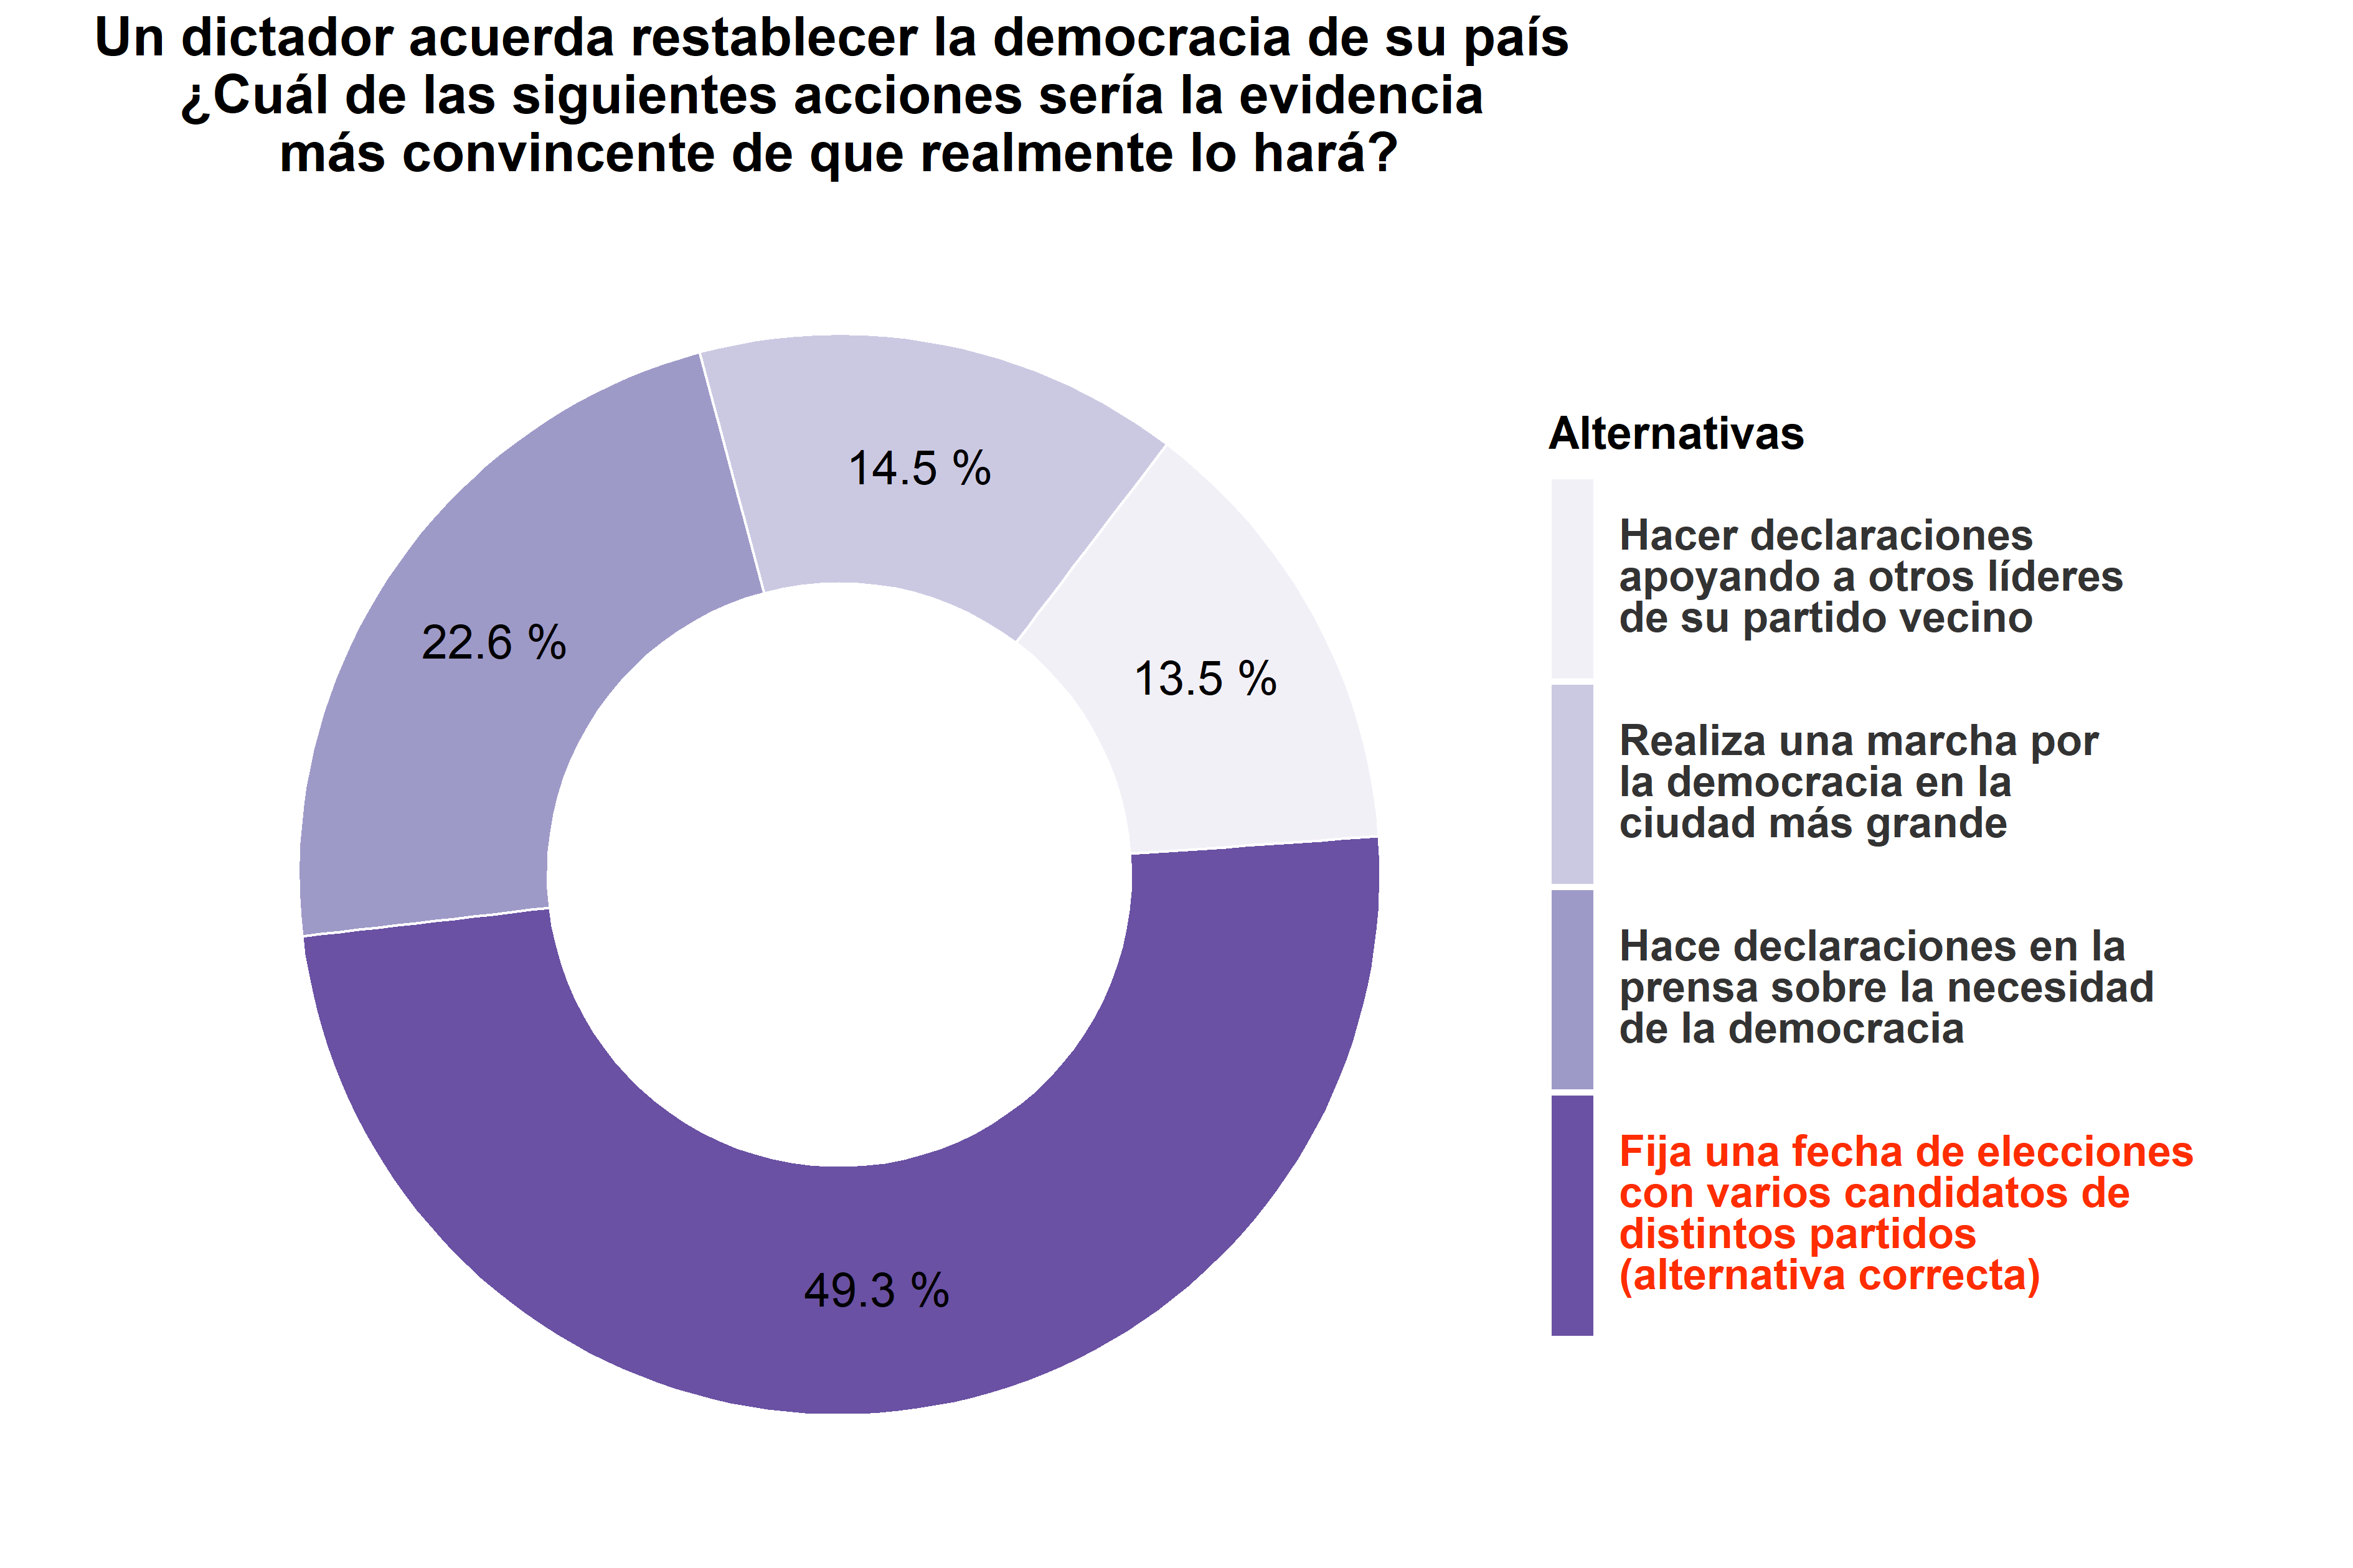
\includegraphics[width=0.8\linewidth,]{images/ccivico_5} 

}

\caption{Acción que demuestra que un dictador restablecerá la democracia}\label{fig:unnamed-chunk-9}
\end{figure}

Un 50.7\% de los estudiantes seleccionó la alternativa correcta. Las respuestas incorrectas se concentraron en una alternativa en particular, la cual fue seleccionada por el 24\% de los estudiantes.

\begin{center}\rule{0.5\linewidth}{0.5pt}\end{center}

\begin{figure}[!ht]

{\centering 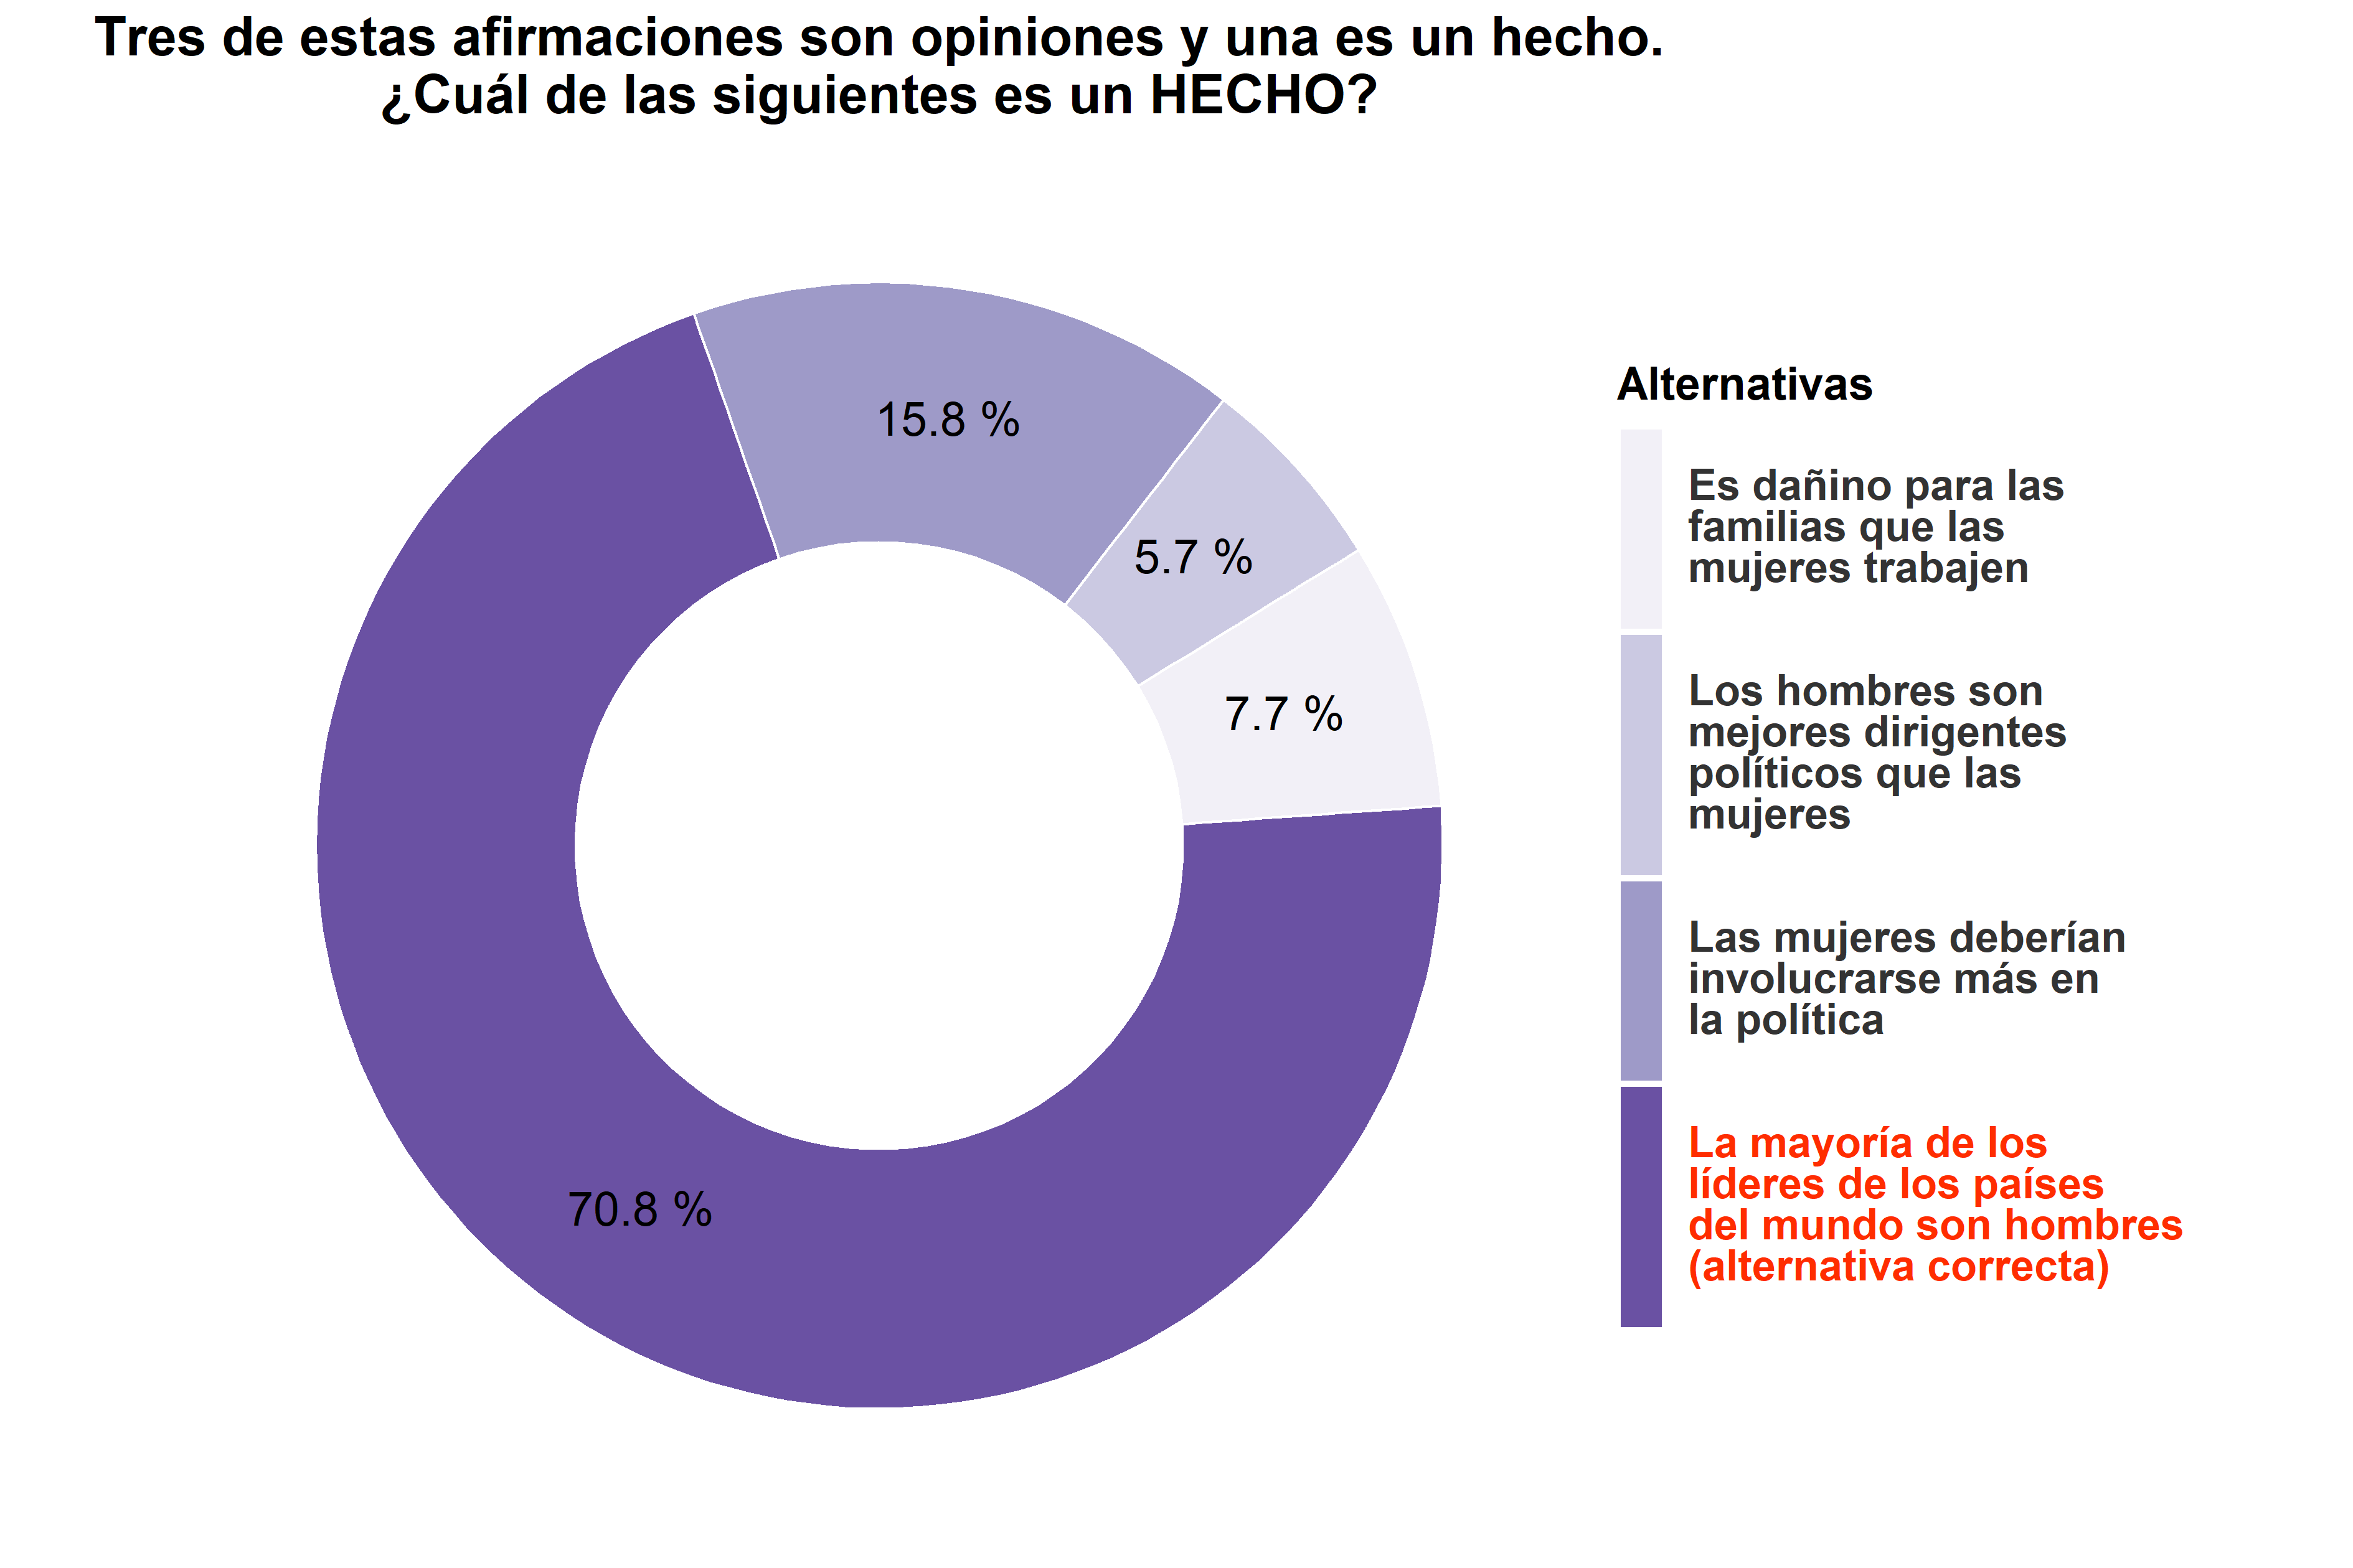
\includegraphics[width=0.8\linewidth,]{images/ccivico_6} 

}

\caption{Afirmación que corresponde a un hecho}\label{fig:unnamed-chunk-10}
\end{figure}

La mayoría de los estudiantes (un 75.2\%) respondió de forma correcta. Si bien son pocos los estudiantes que se distrajeron con las otras alternativas, hubo una alternativa que concentró parte importante de las respuestas incorrectas (un 14.2\%).

\begin{center}\rule{0.5\linewidth}{0.5pt}\end{center}

\begin{figure}[!ht]

{\centering 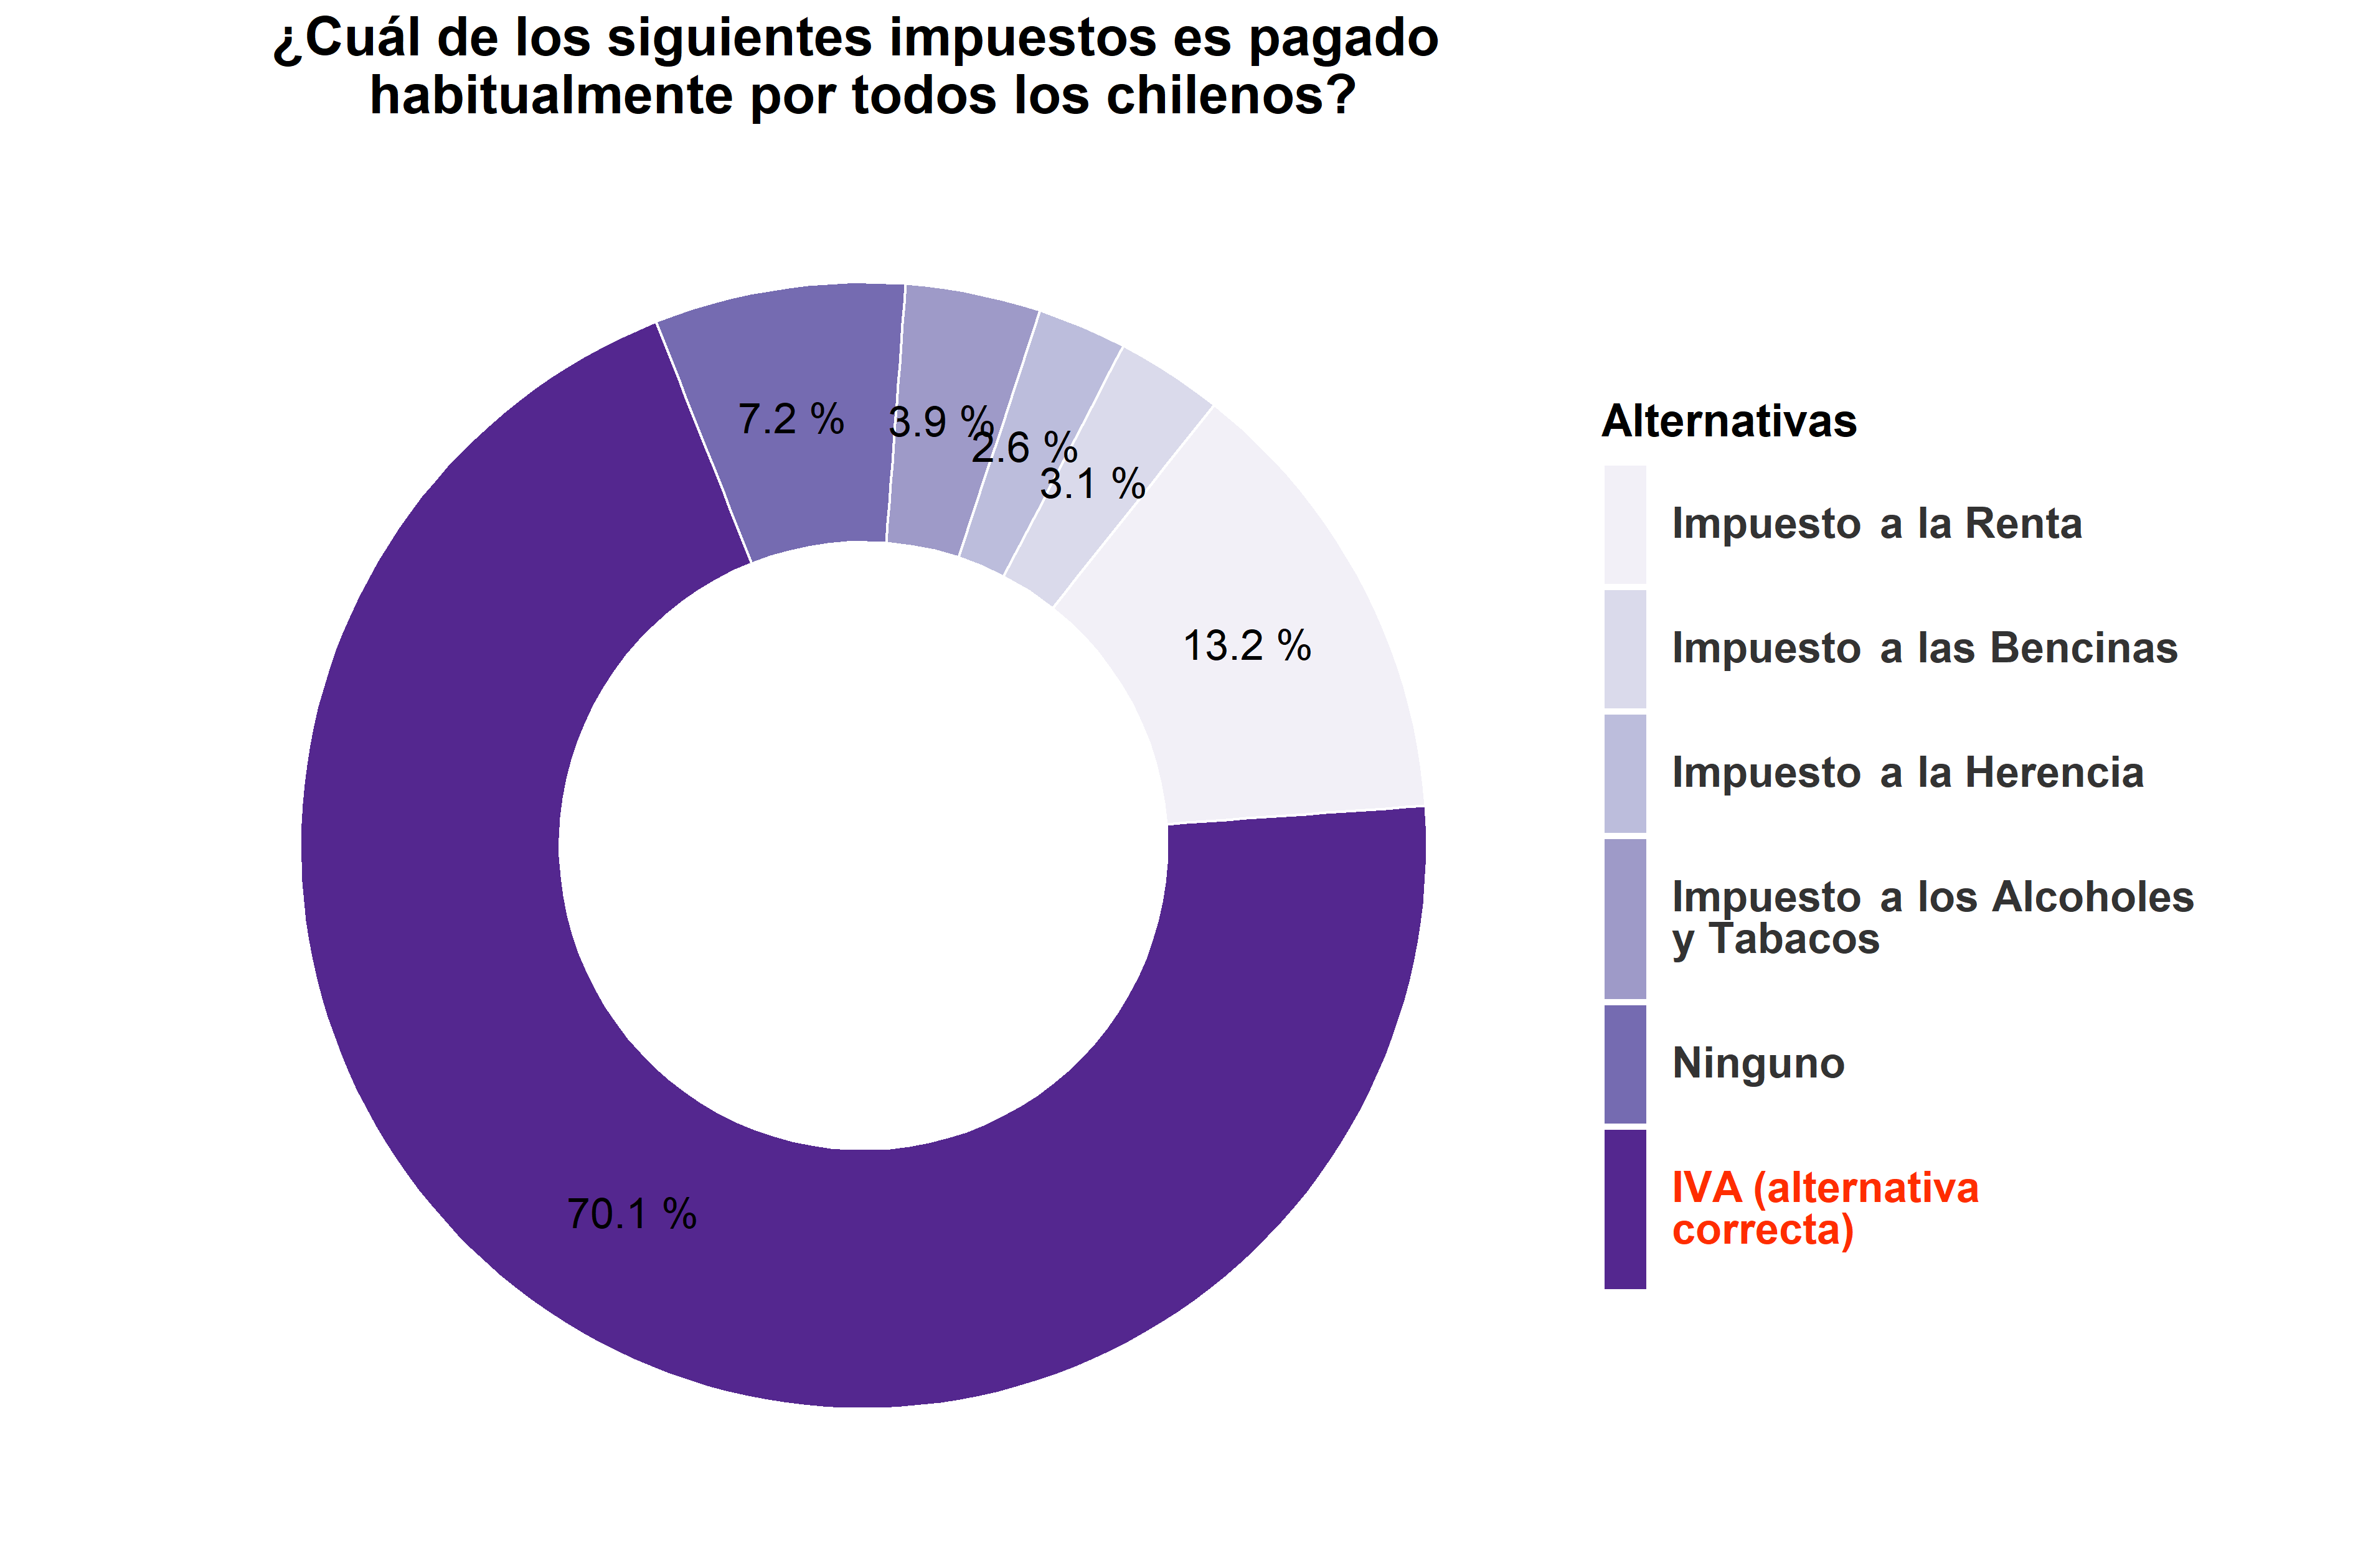
\includegraphics[width=0.8\linewidth,]{images/ccivico_7} 

}

\caption{Impuesto pagado por todos los chilenos}\label{fig:unnamed-chunk-11}
\end{figure}

La mayoría de los estudiantes (un 70.1\%) seleccionó la alternativa correcta. En relación con las respuestas incorrectas, una alternativa en particular concentró la mayor parte de las respuestas restantes, siendo seleccionada por el 13.2\% de los estudiantes.

\begin{center}\rule{0.5\linewidth}{0.5pt}\end{center}

\begin{figure}[!ht]

{\centering 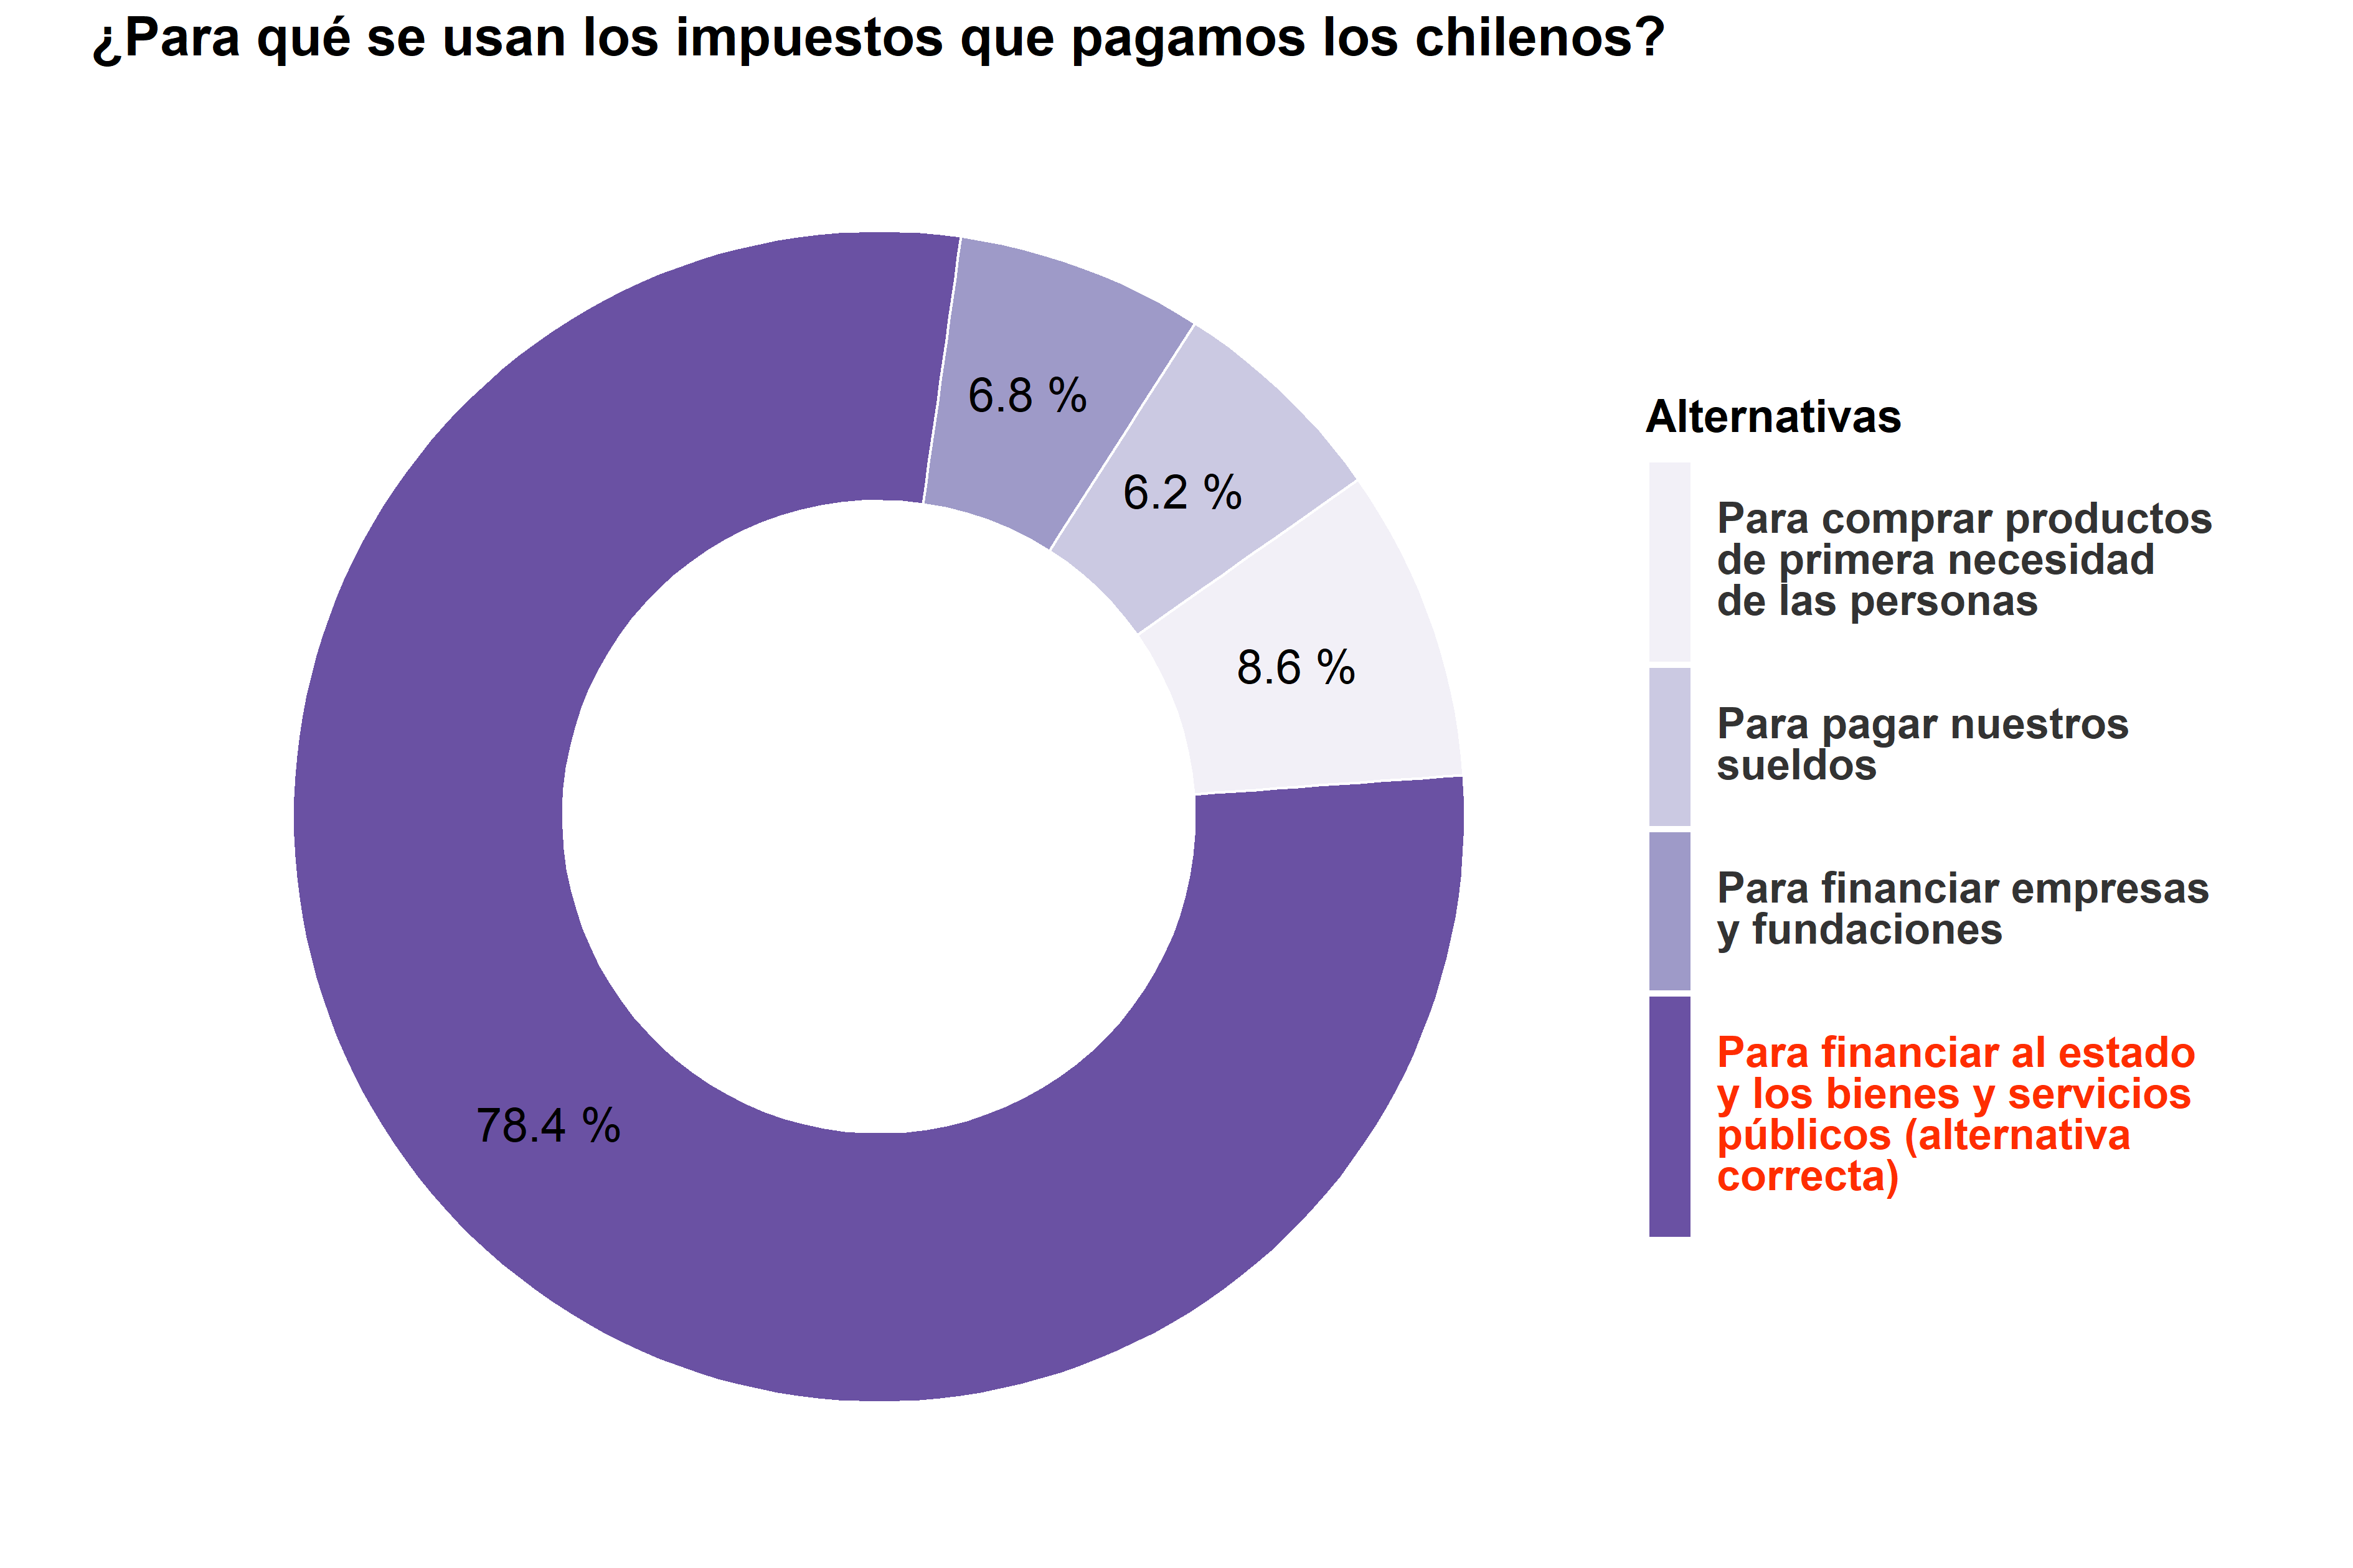
\includegraphics[width=0.8\linewidth,]{images/ccivico_8} 

}

\caption{Uso de los impuestos en Chile}\label{fig:unnamed-chunk-12}
\end{figure}

La mayoría de los estudiantes (un 80.9\%) respondió correctamente. Fueron pocos los que se distrajeron con las otras alternativas y las respuestas incorrectas no se concentraron en una alternativa en particular.

\begin{center}\rule{0.5\linewidth}{0.5pt}\end{center}

\begin{figure}[!ht]

{\centering 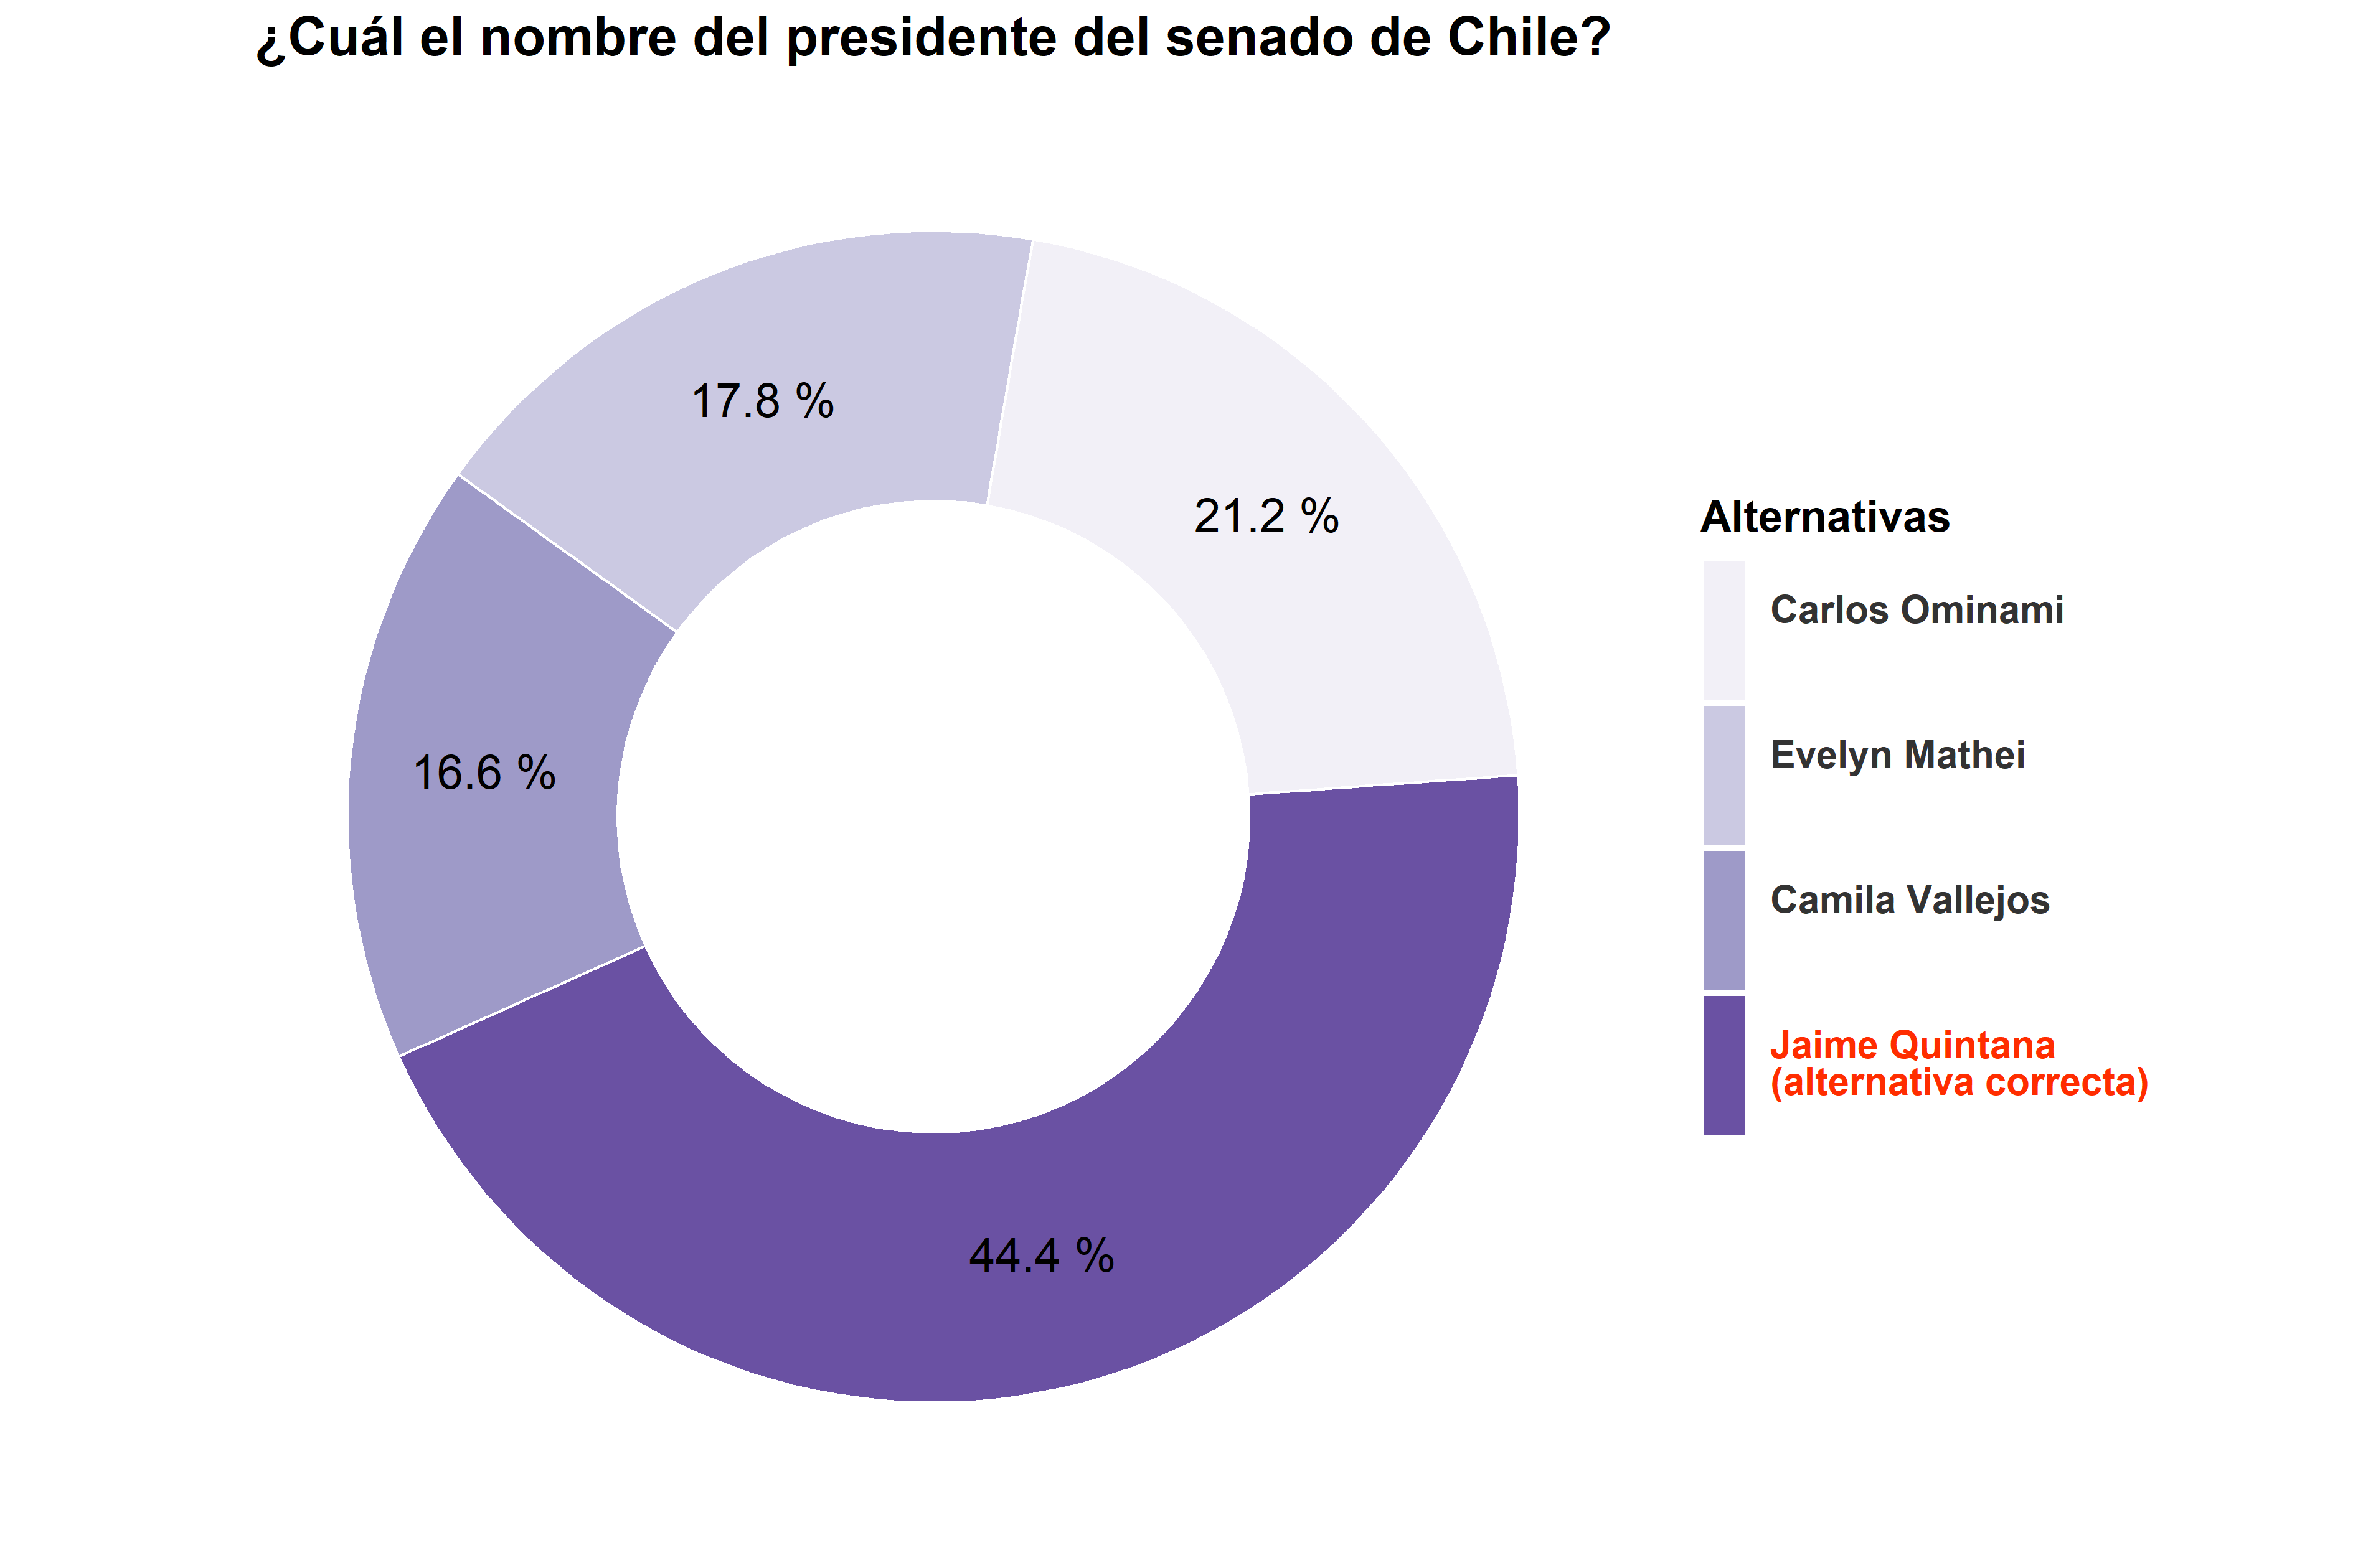
\includegraphics[width=0.8\linewidth,]{images/ccivico_9} 

}

\caption{Presidente del senado de Chile}\label{fig:unnamed-chunk-13}
\end{figure}

Un 44.6\% de los estudiantes seleccionó la alternativa correcta. Las respuestas incorrectas no se concentraron en una alternativa en particular.

\begin{center}\rule{0.5\linewidth}{0.5pt}\end{center}

\begin{figure}[!ht]

{\centering 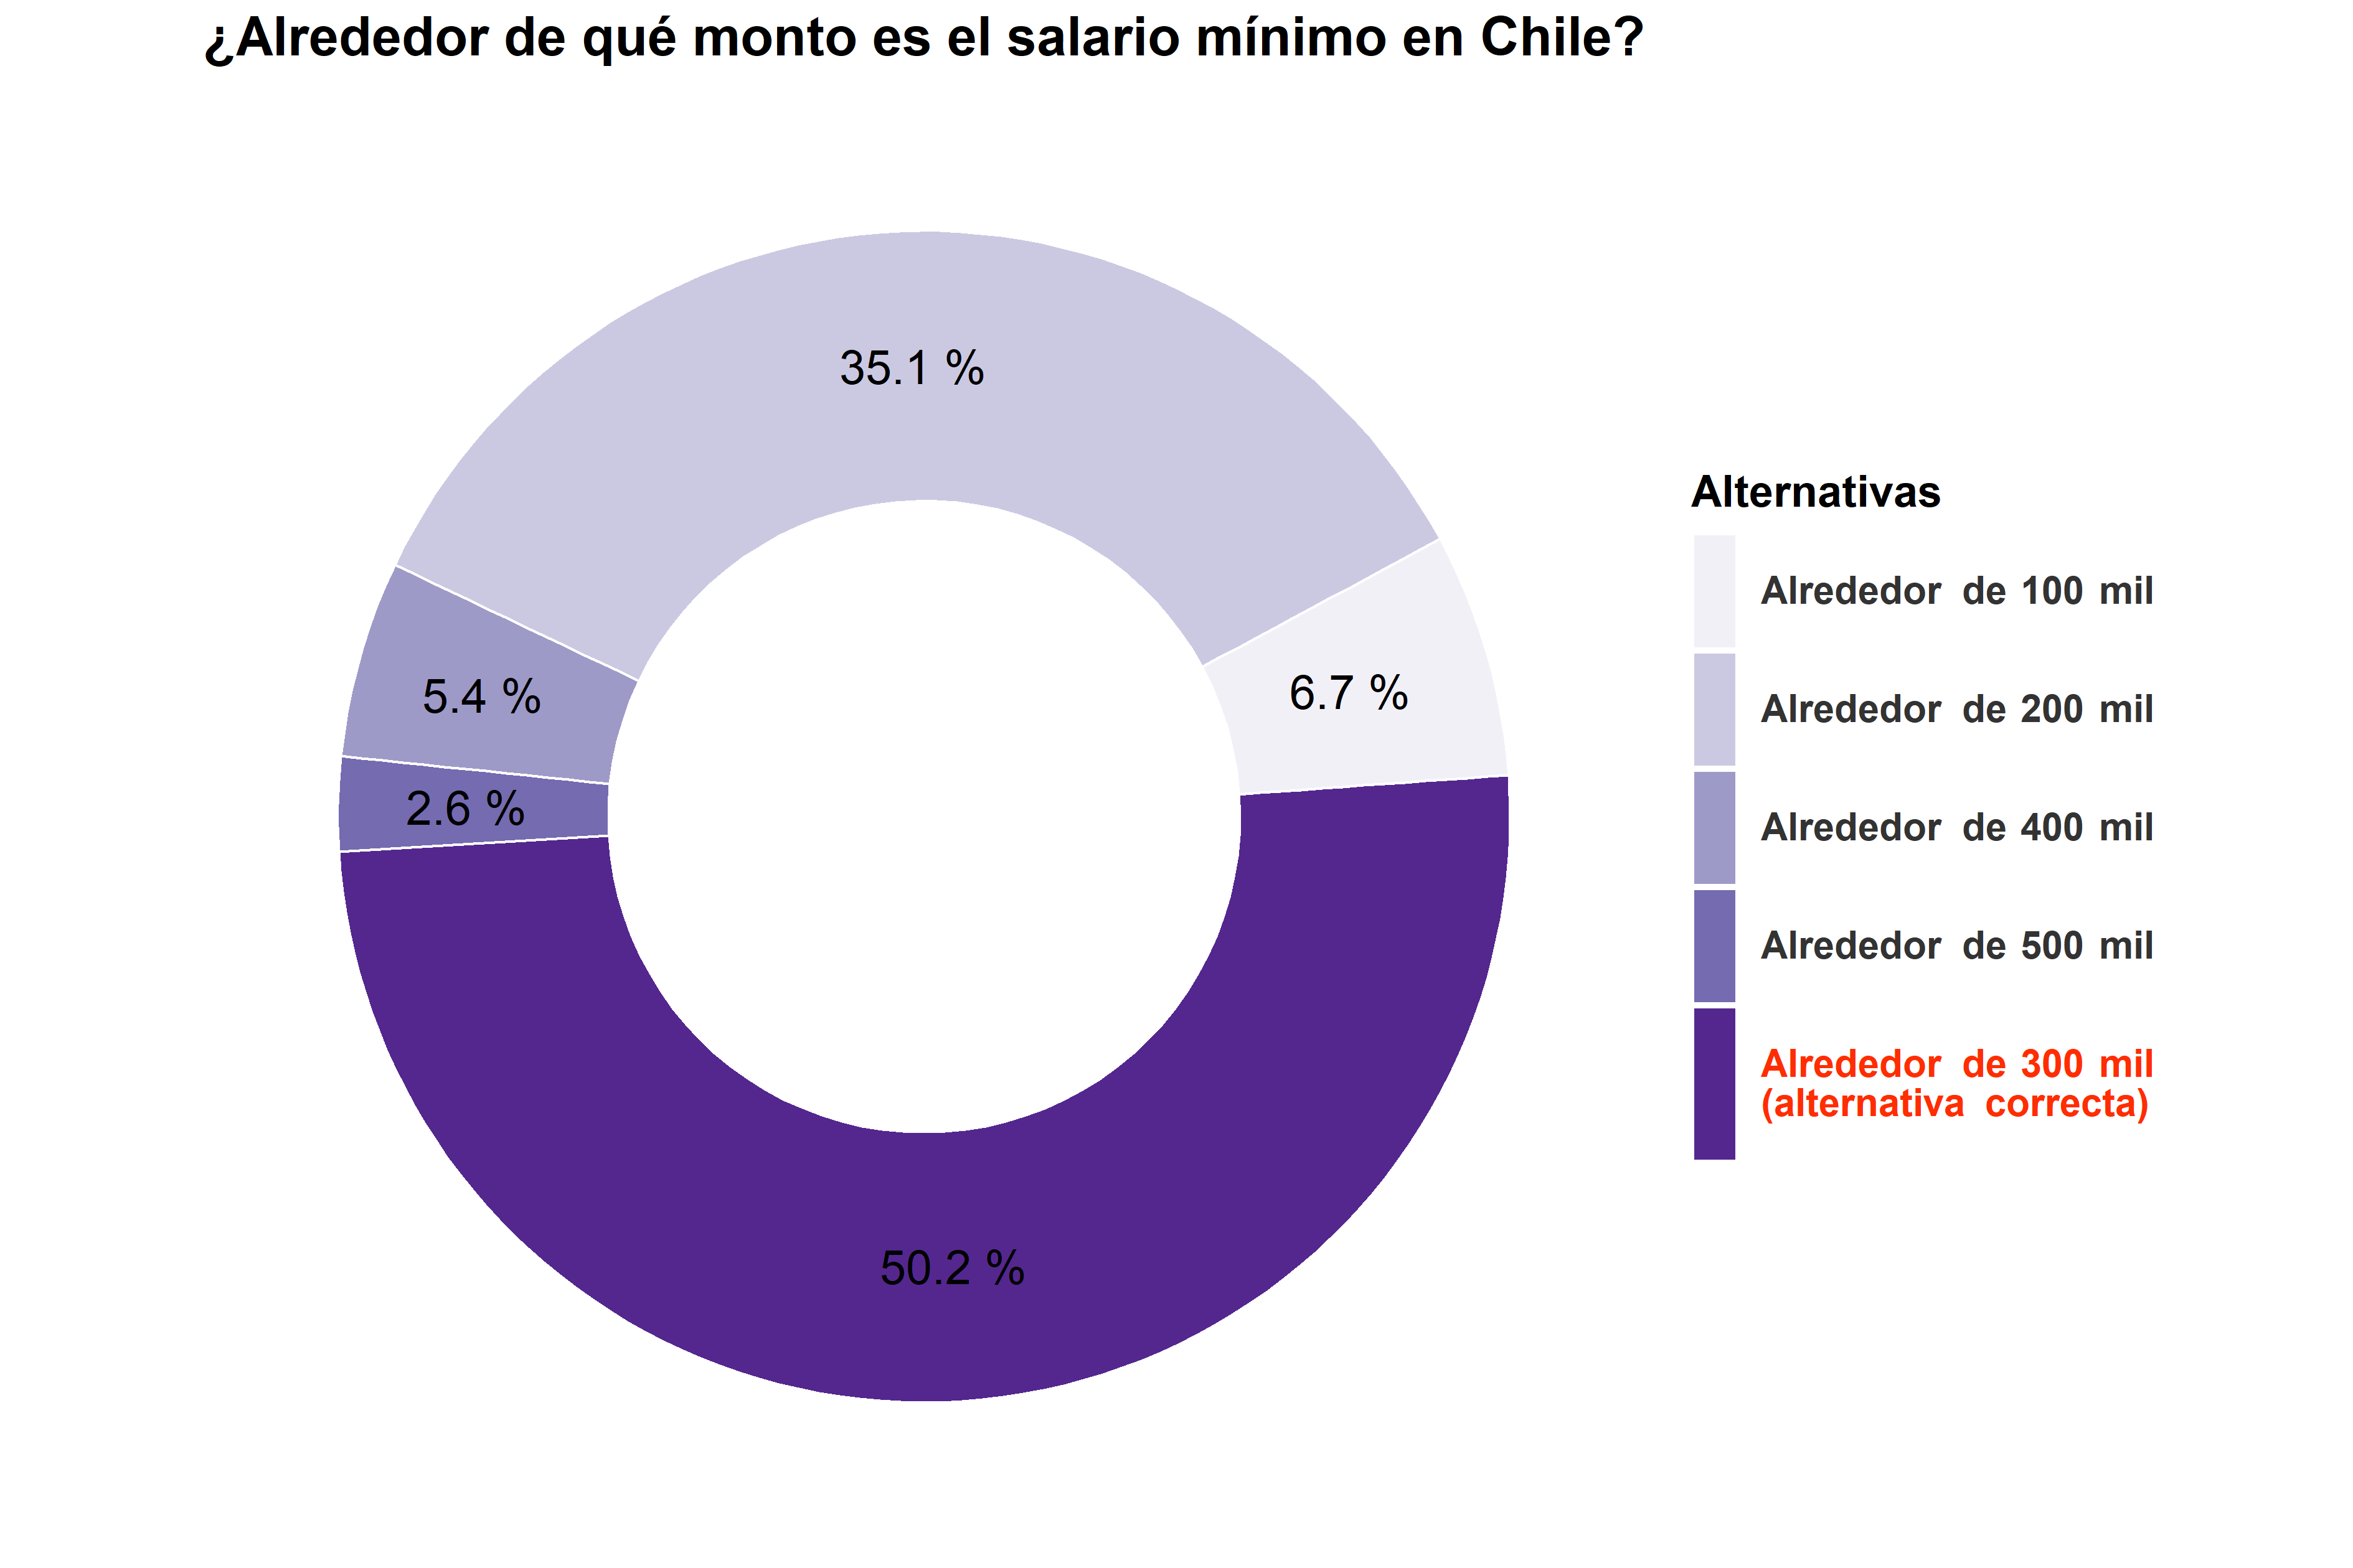
\includegraphics[width=0.8\linewidth,]{images/ccivico_10} 

}

\caption{Salario mínimo en Chile}\label{fig:unnamed-chunk-14}
\end{figure}

La mayoría de los estudiantes (un 50.2\%) respondió de forma correcta. Las respuestas incorrectas se concentraron en una de las alternativas, la cual fue seleccionada por el 35.1\% de los estudiantes.

\begin{center}\rule{0.5\linewidth}{0.5pt}\end{center}

\begin{figure}[!ht]

{\centering 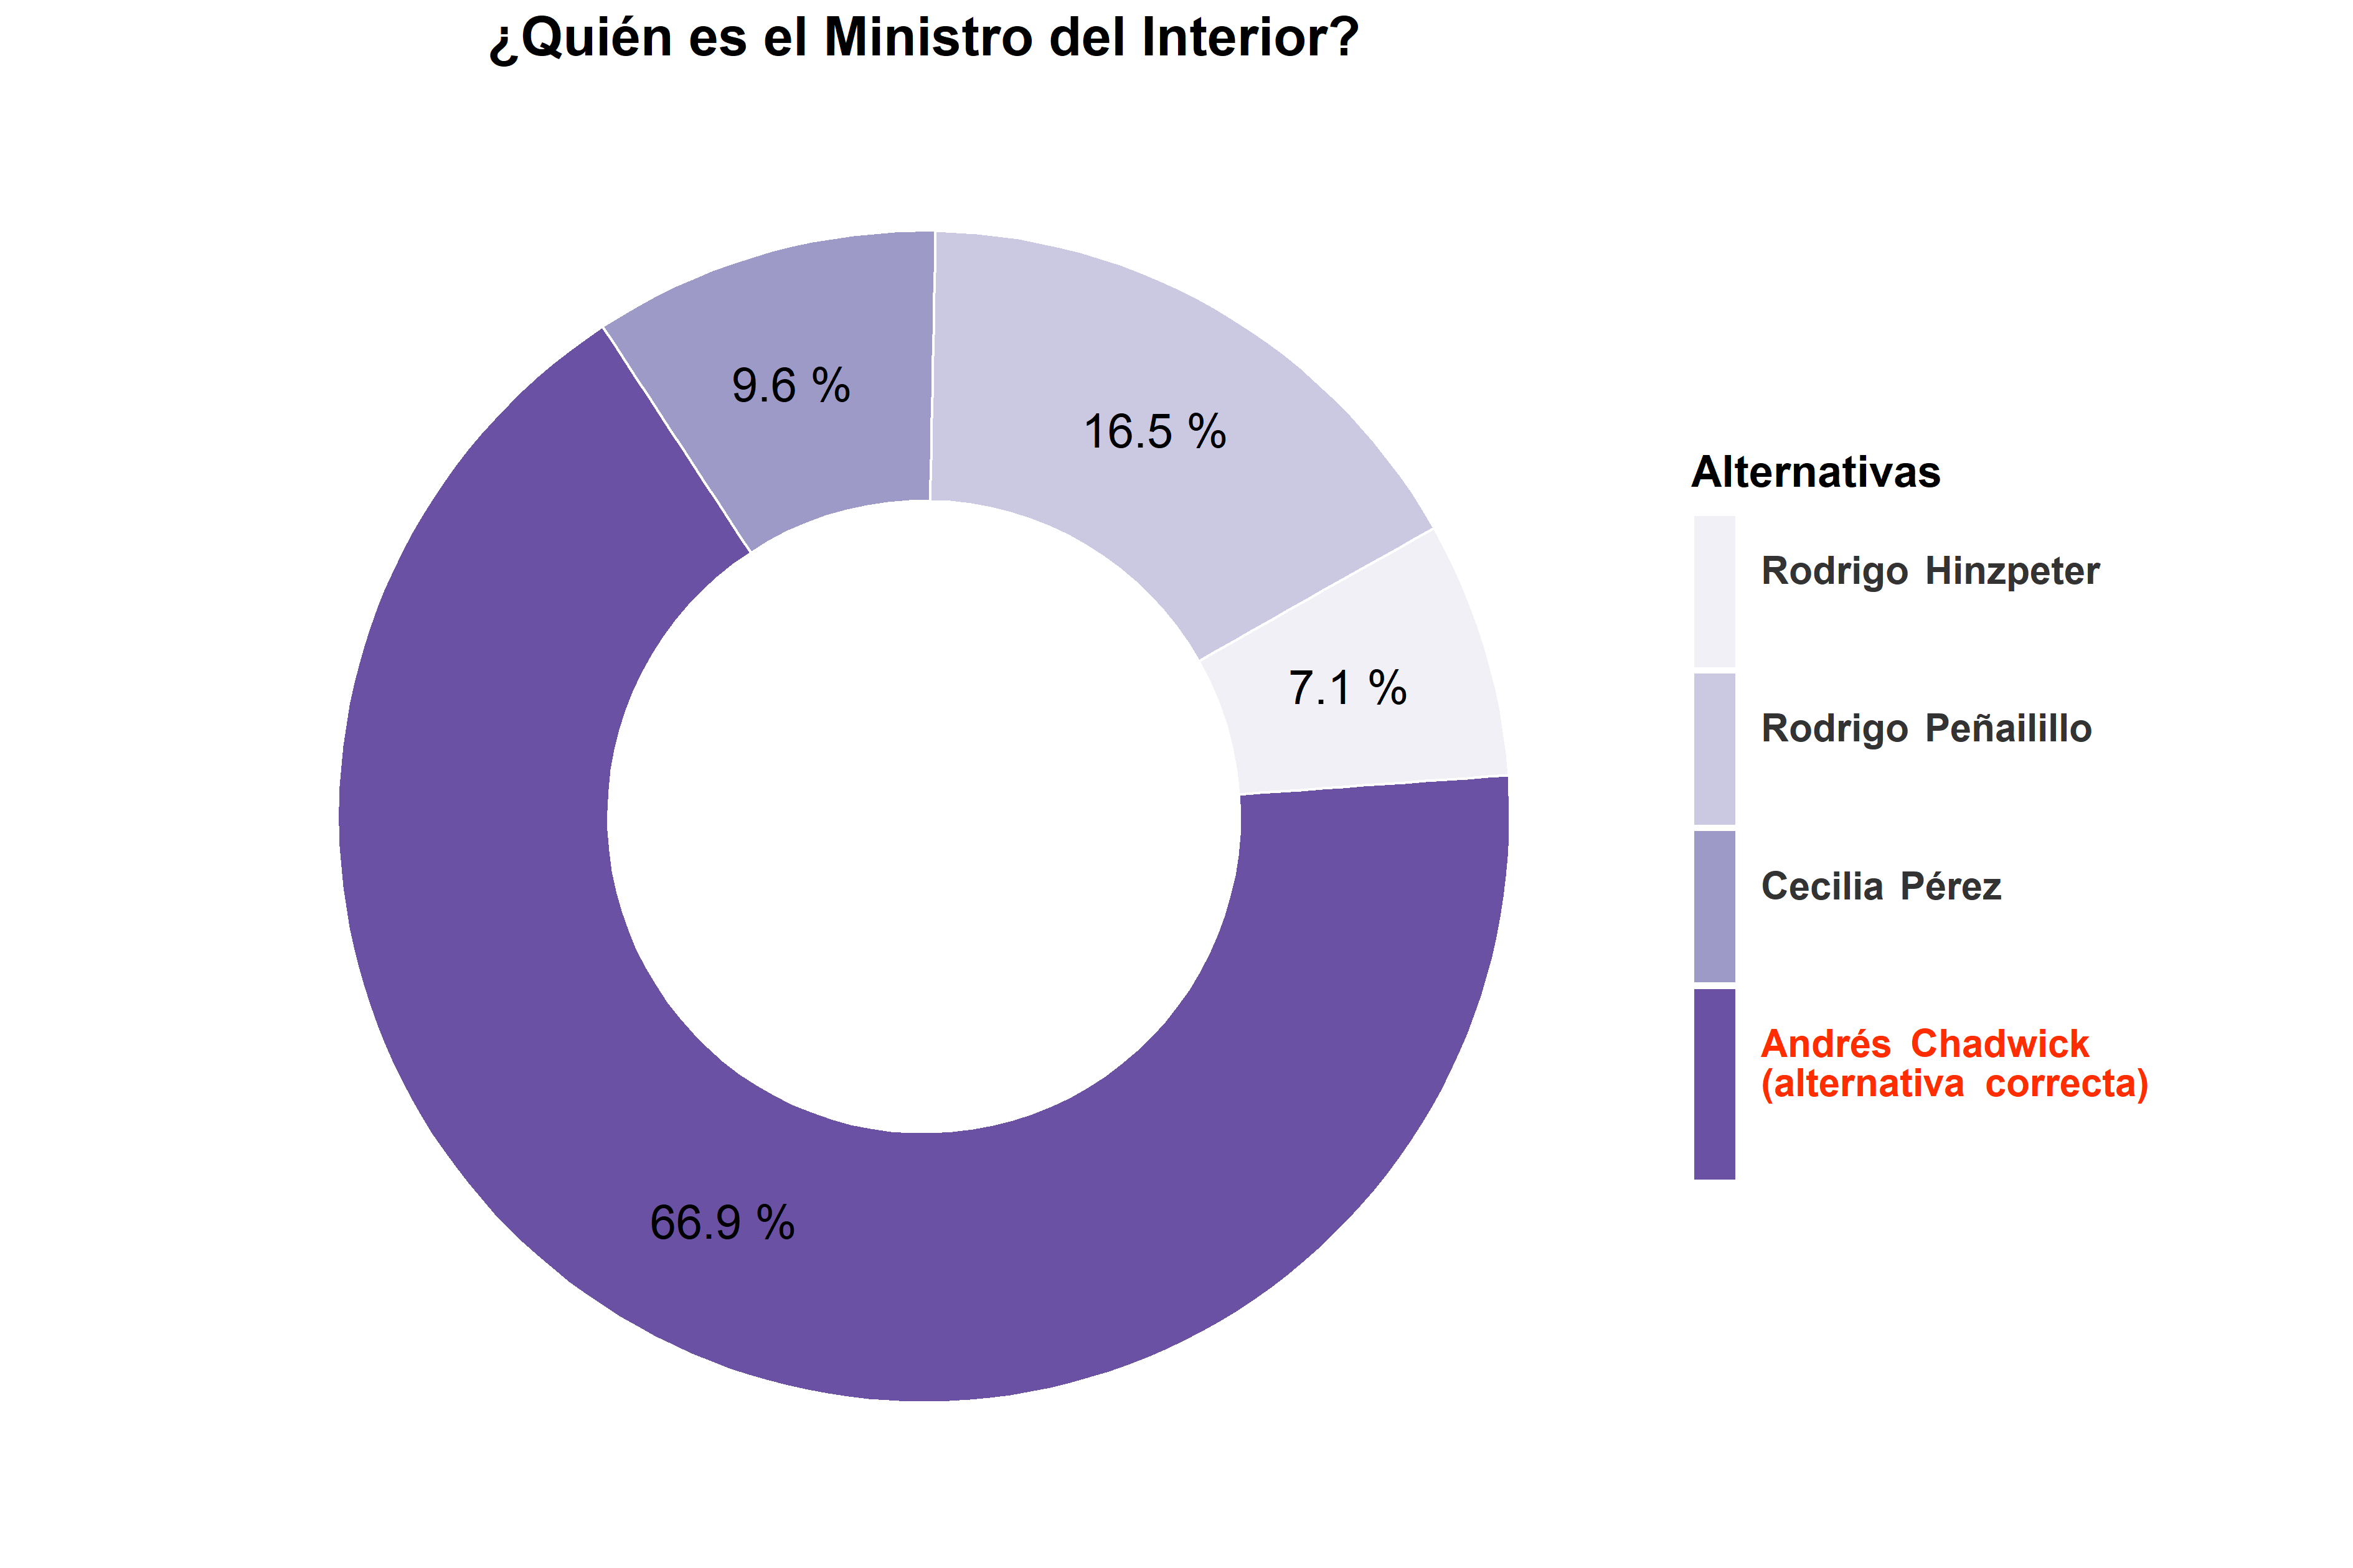
\includegraphics[width=0.8\linewidth,]{images/ccivico_11} 

}

\caption{Ministro del interior}\label{fig:unnamed-chunk-15}
\end{figure}

La mayoría de los estudiantes (un 66.9\%) respondió correctamente. Si bien fueron pocos los estudiantes que se distrajeron con las alternativas incorrectas, hubo una alternativa en particular que concentró parte importante de las respuestas restantes (un 16.5\%).

\begin{center}\rule{0.5\linewidth}{0.5pt}\end{center}

\begin{figure}[!ht]

{\centering 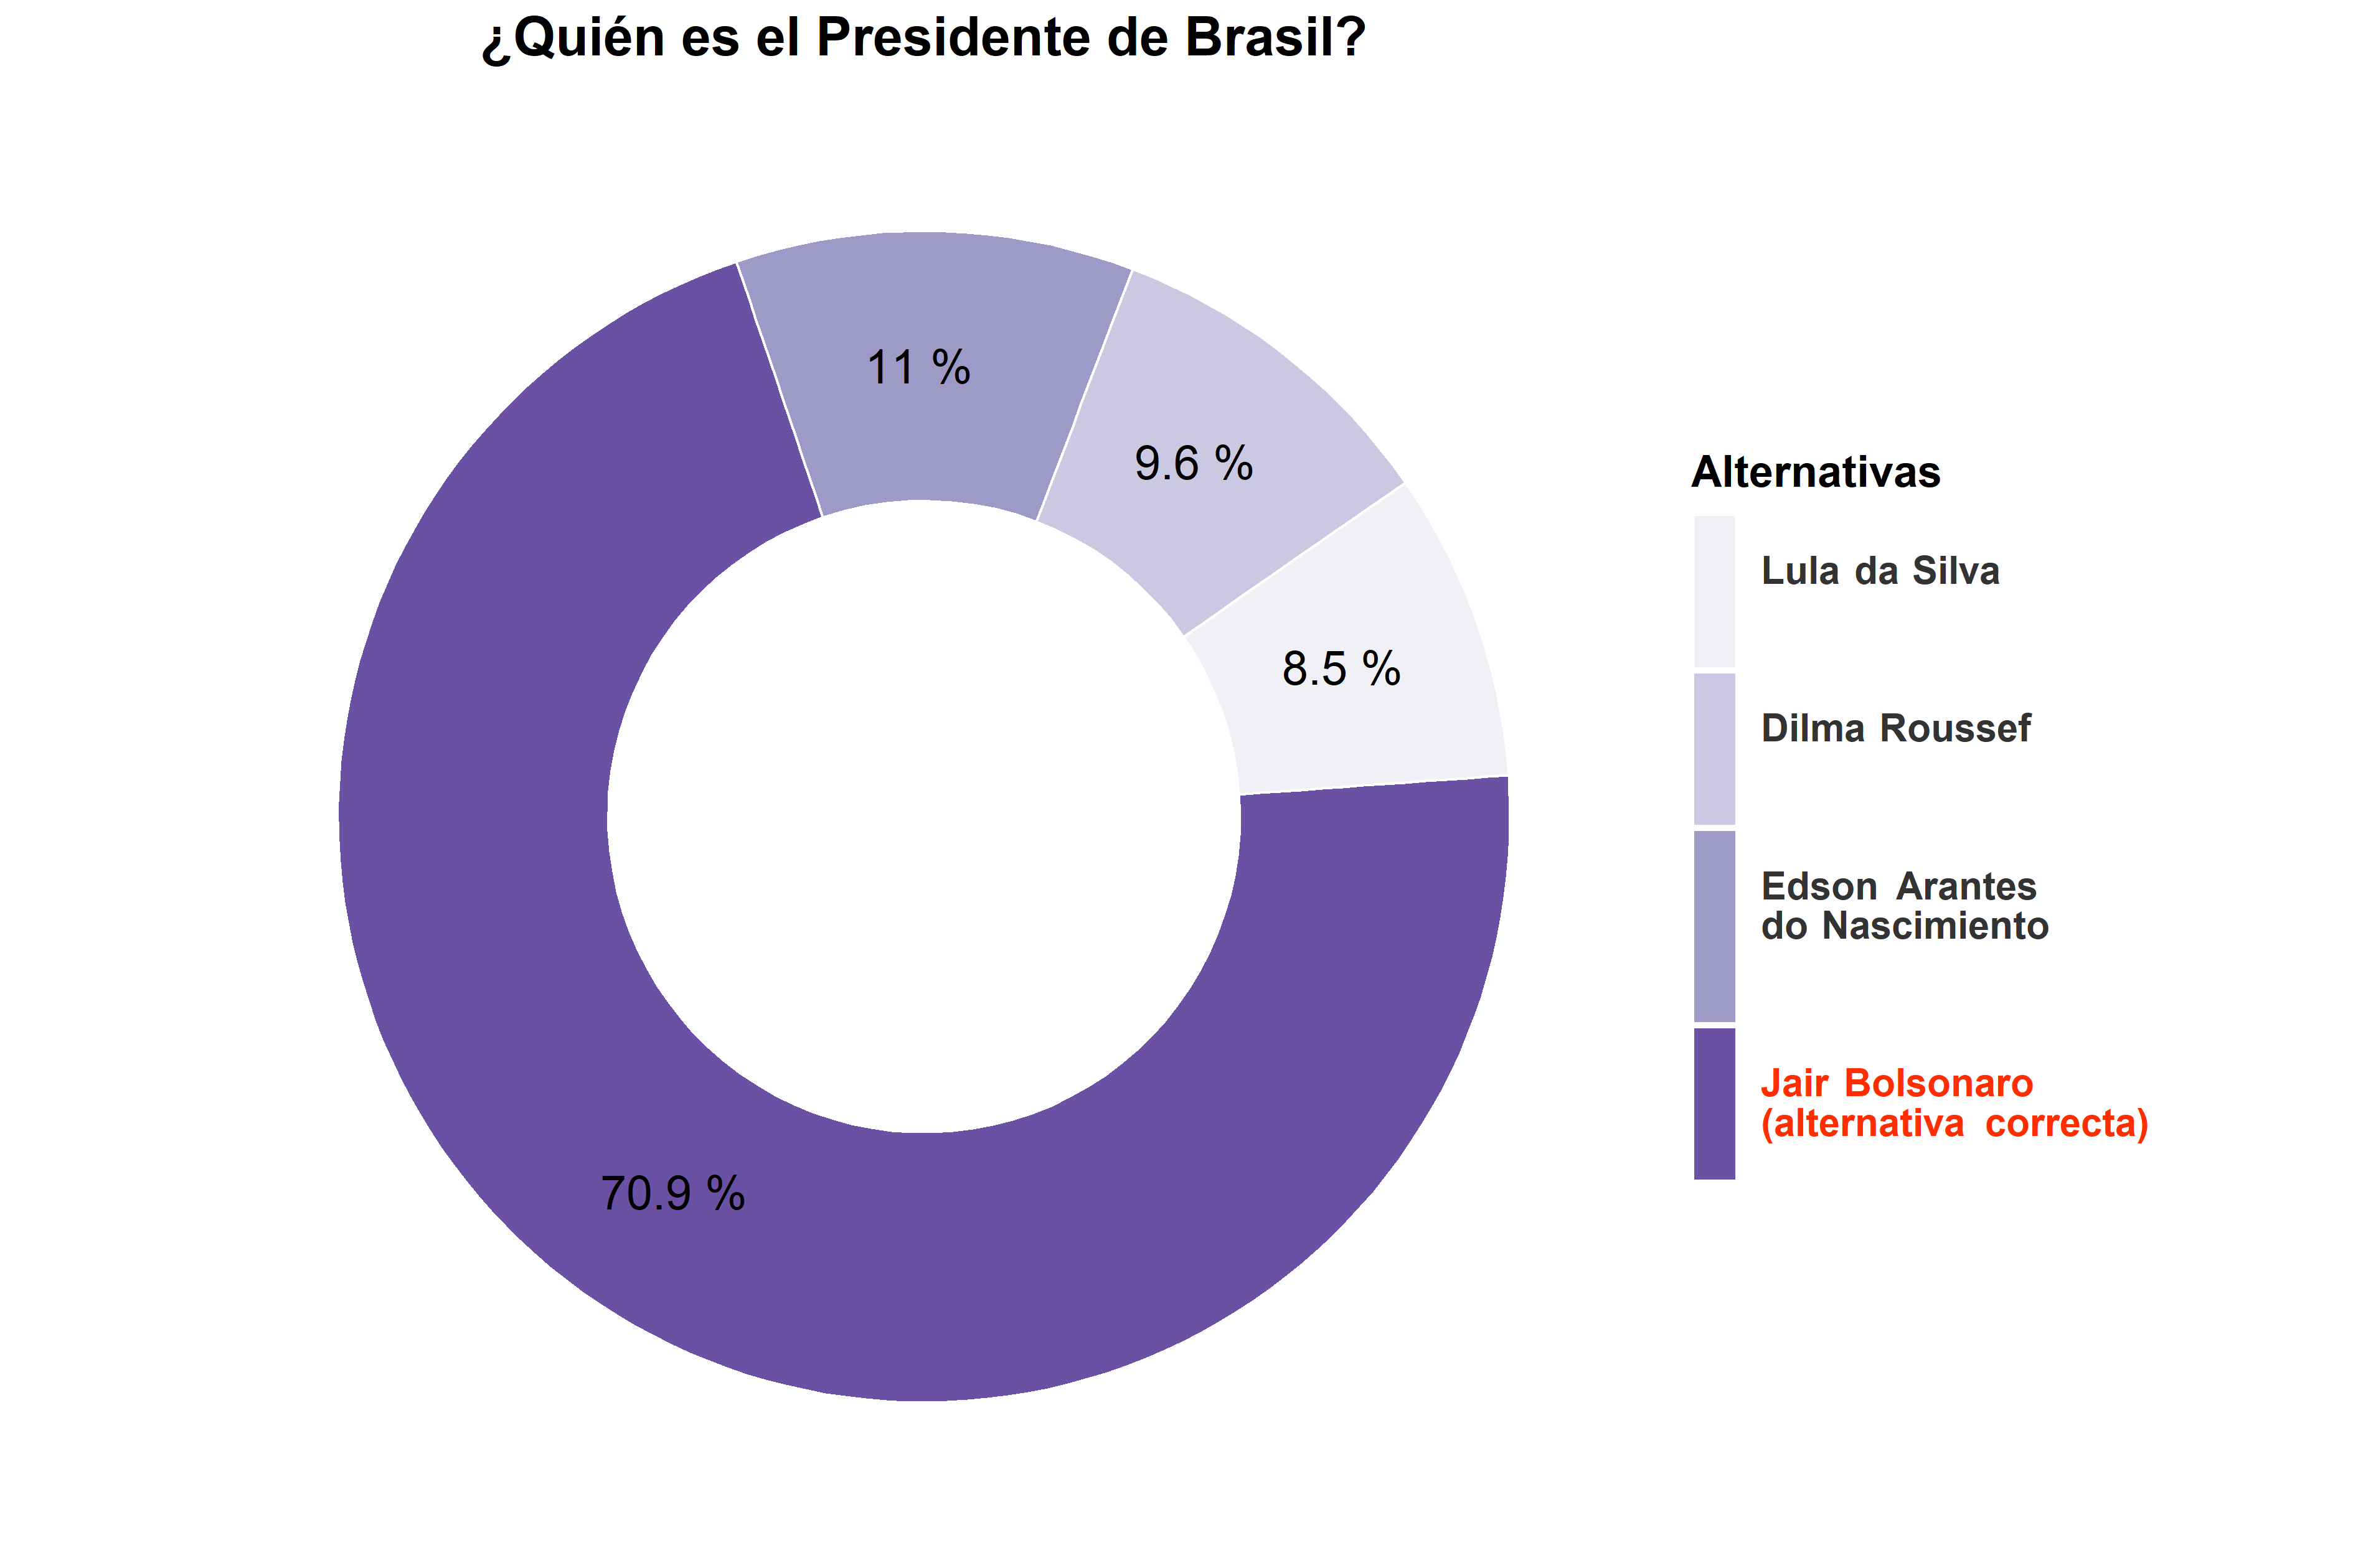
\includegraphics[width=0.8\linewidth,]{images/ccivico_12} 

}

\caption{Presidente de Brasil}\label{fig:unnamed-chunk-16}
\end{figure}

La mayoría de los estudiantes (un 70.9\%) seleccionó la alternativa correcta. Las respuestas incorrectas se distribuyeron de forma pareja entre las alternativas restantes.

\begin{center}\rule{0.5\linewidth}{0.5pt}\end{center}

\begin{figure}[!ht]

{\centering 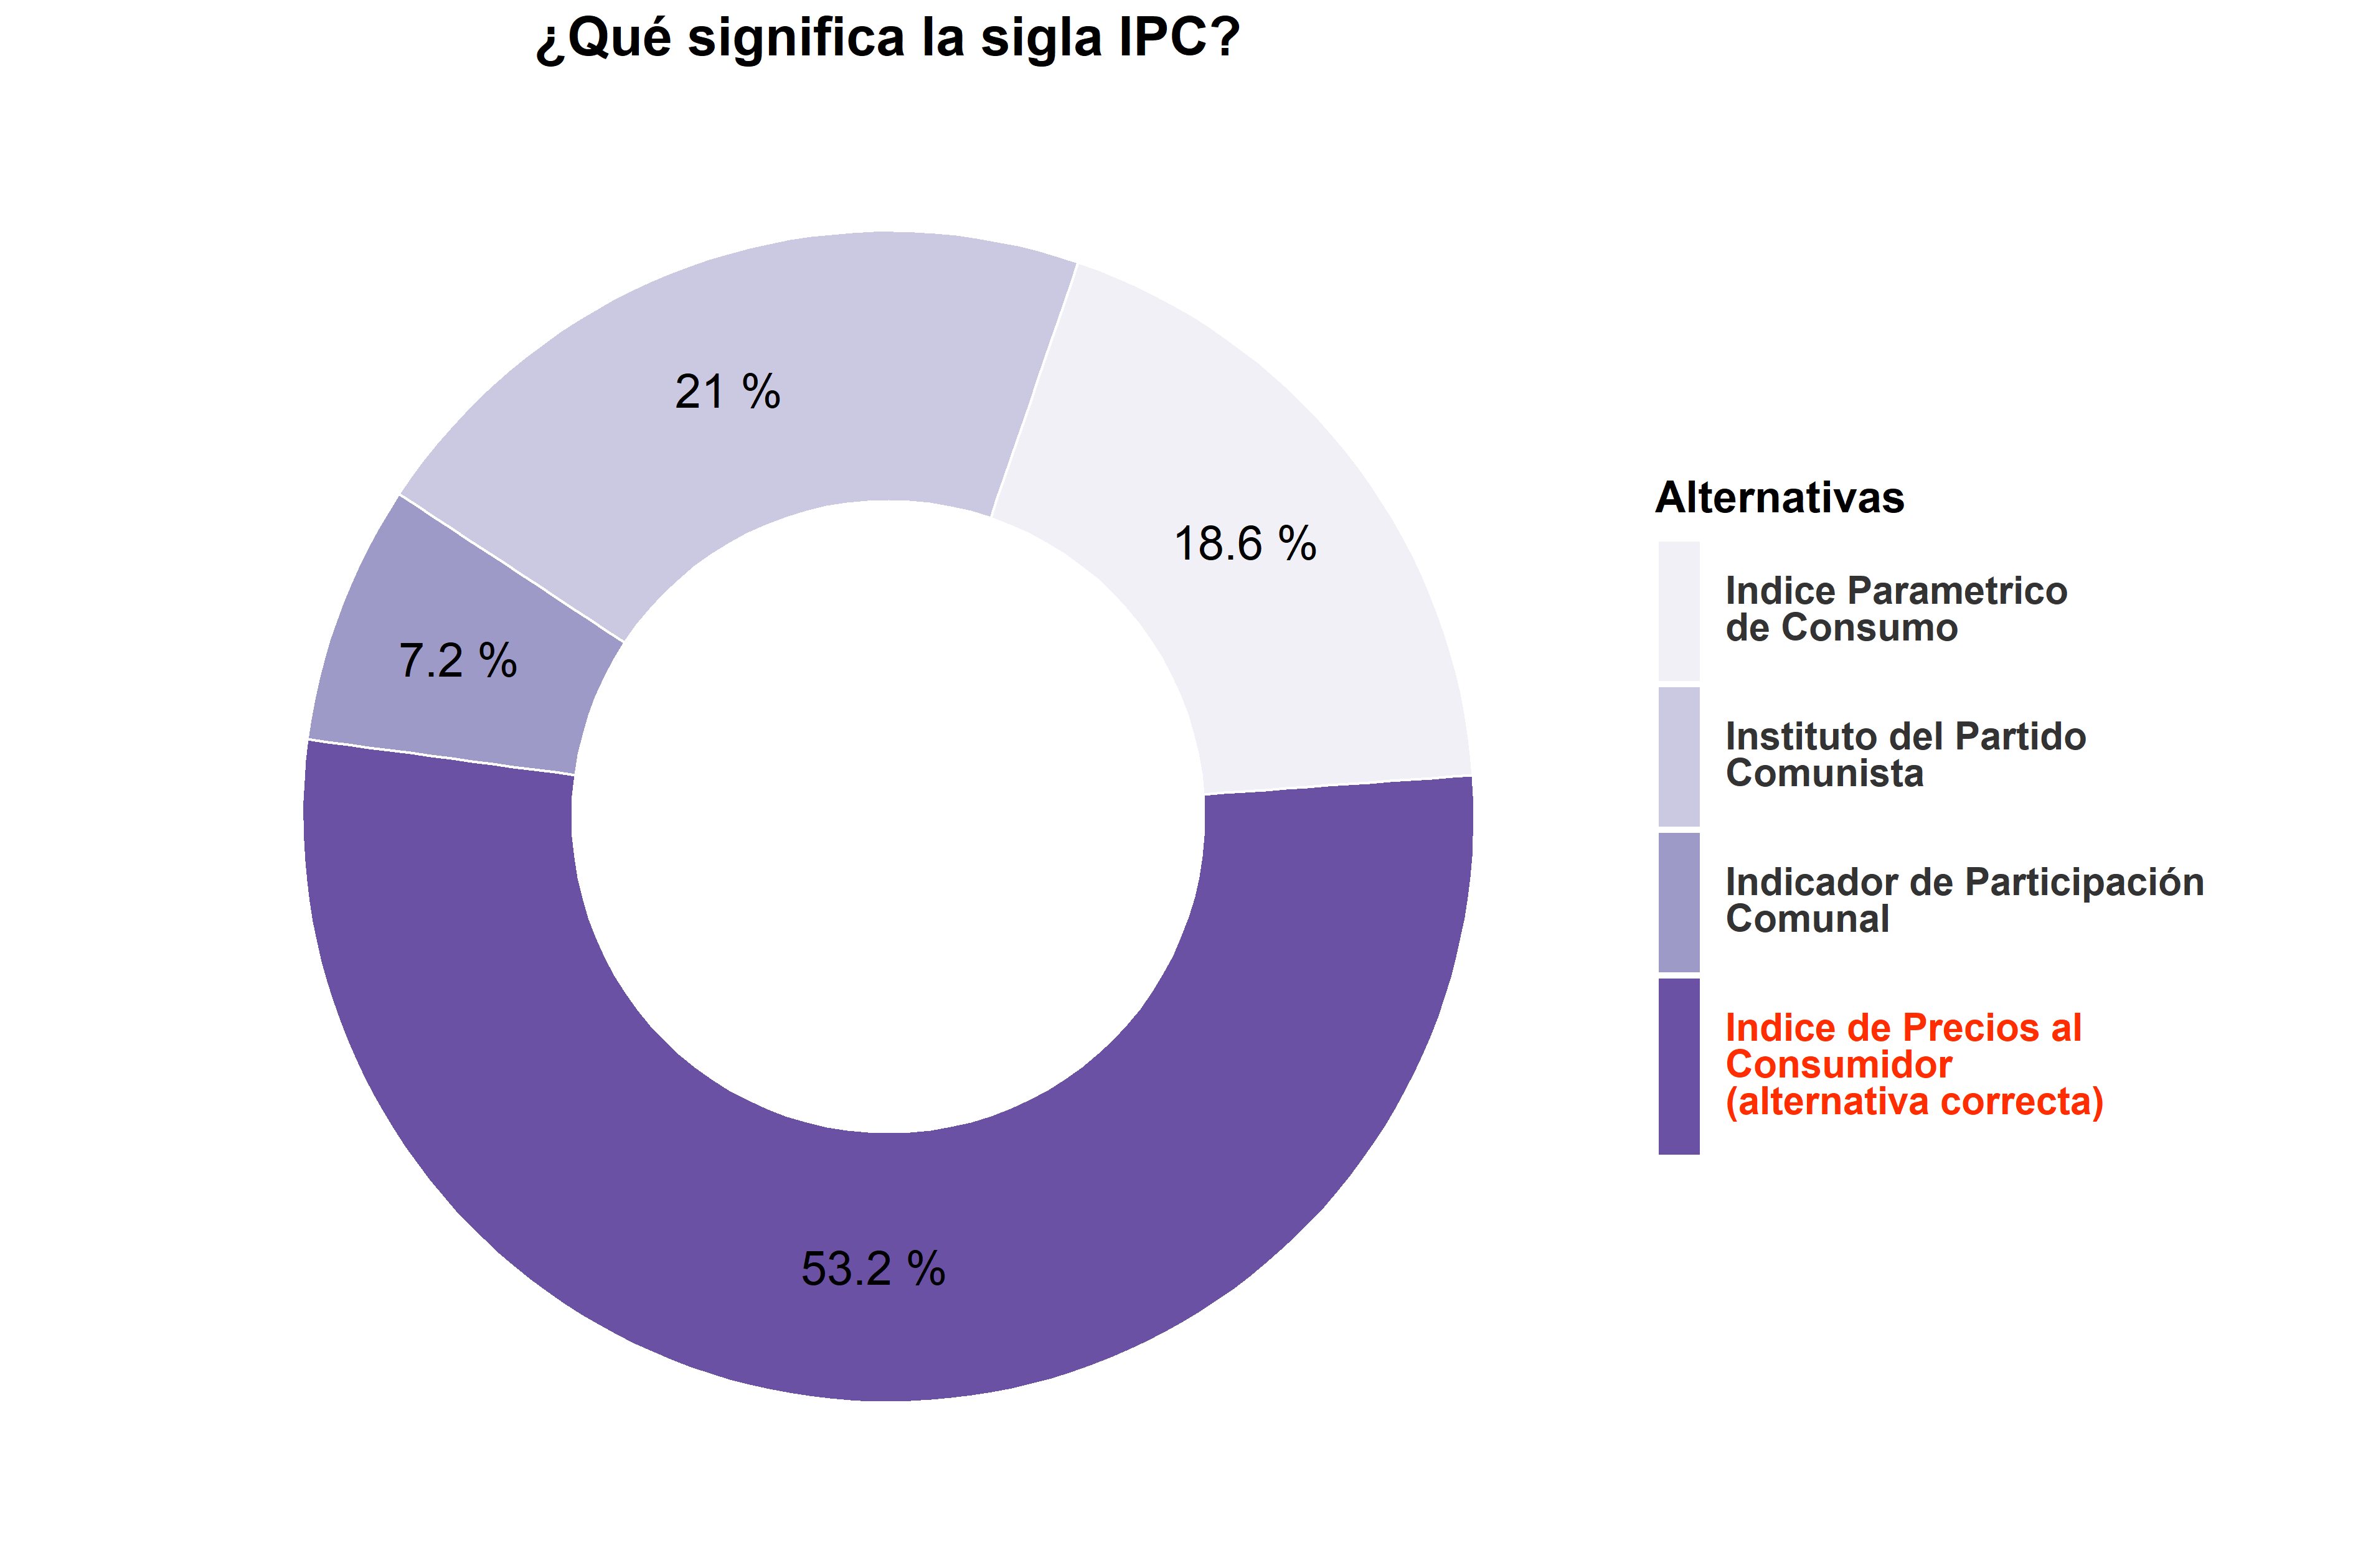
\includegraphics[width=0.8\linewidth,]{images/ccivico_13} 

}

\caption{Significado IPC}\label{fig:unnamed-chunk-17}
\end{figure}

La mayoría de los estudiantes (un 56\%) respondió de forma correcta. Las respuestas incorrectas se concentraron principalmente en dos alternativas, que fueron seleccionadas por el 19.9\% y el 18.1\% de los estudiantes.

\begin{center}\rule{0.5\linewidth}{0.5pt}\end{center}

\begin{figure}[!ht]

{\centering 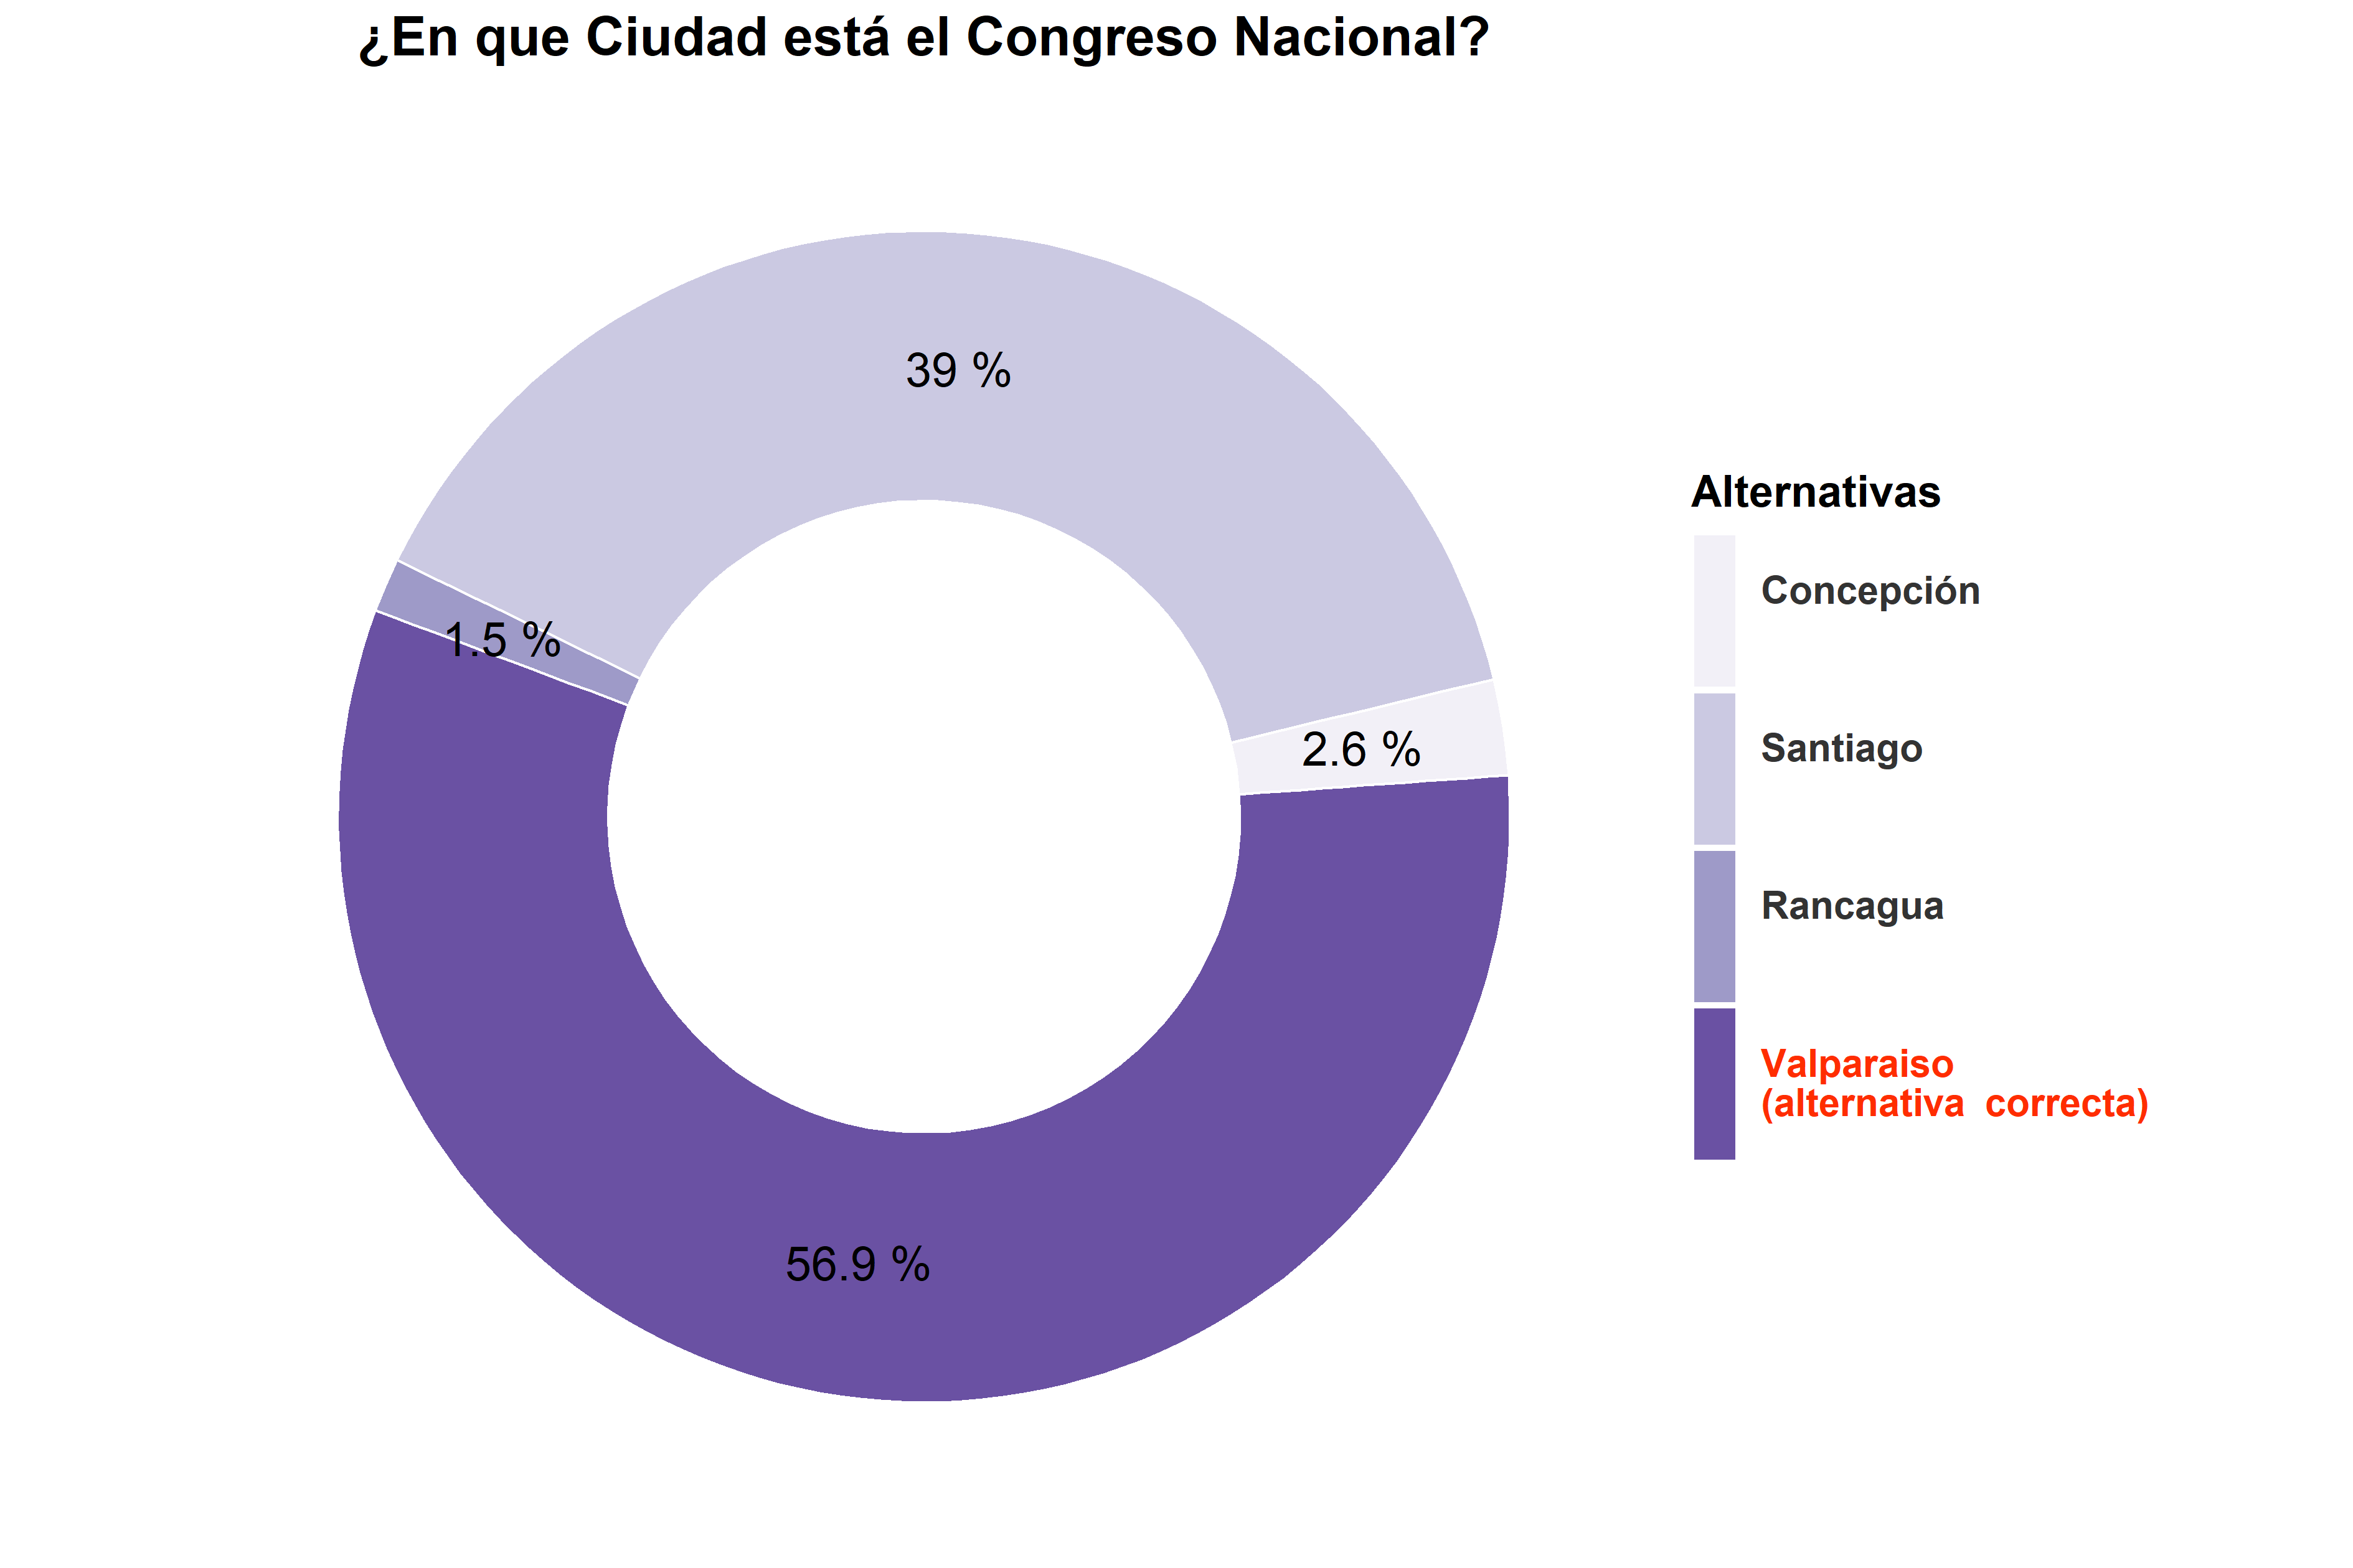
\includegraphics[width=0.8\linewidth,]{images/ccivico_14} 

}

\caption{Localización del Congreso}\label{fig:unnamed-chunk-18}
\end{figure}

Un 56.9\% de los estudiantes respondió correctamente. Casi la totalidad de respuestas restantes se concentró en una de las alternativas incorrectas (un 39\%).

\begin{center}\rule{0.5\linewidth}{0.5pt}\end{center}

\hypertarget{comparaciuxf3n-conocimiento-cuxedvico-paces-iccs-2009}{%
\section{Comparación conocimiento cívico PACES / ICCS 2009}\label{comparaciuxf3n-conocimiento-cuxedvico-paces-iccs-2009}}

Como se enuncio anteriormente, las seis preguntas que se presentarán en esta subsección corresponden a indicadores provenientes del estudio ICCS que evalúan distintas aristas del \textbf{\emph{conocimiento cívico conceptual}}. Se comparará el patrón de respuesta de los estudiantes de 8°básico, encuestados en el estudio ICCS el año 2009, con las respuestas de los estudiantes de 2°medio, encuestados por este equipo de investigación el año 2019. Cabe destacar que la comparación se realizará con las respuestas de estudiantes de 8°básico debido a que es la única población para la cual existen datos disponibles que permiten evaluar el conocimiento cívico de estudiantes en Chile.

En términos generales, al realizar la comparación se puede concluir que hay una tendencia al alza en la identificación de la respuesta correcta en los estudiantes de segundo medio (en 5 de las 6 preguntas) y que, en la mayoría de las preguntas, la alternativa incorrecta que concentraba más casos en las respuestas de los estudiantes de 8°básico es la misma alternativa incorrecta que concentra más casos en las respuestas de los estudiantes de 2°medio.

\begin{center}\rule{0.5\linewidth}{0.5pt}\end{center}

\begin{figure}[!ht]

{\centering 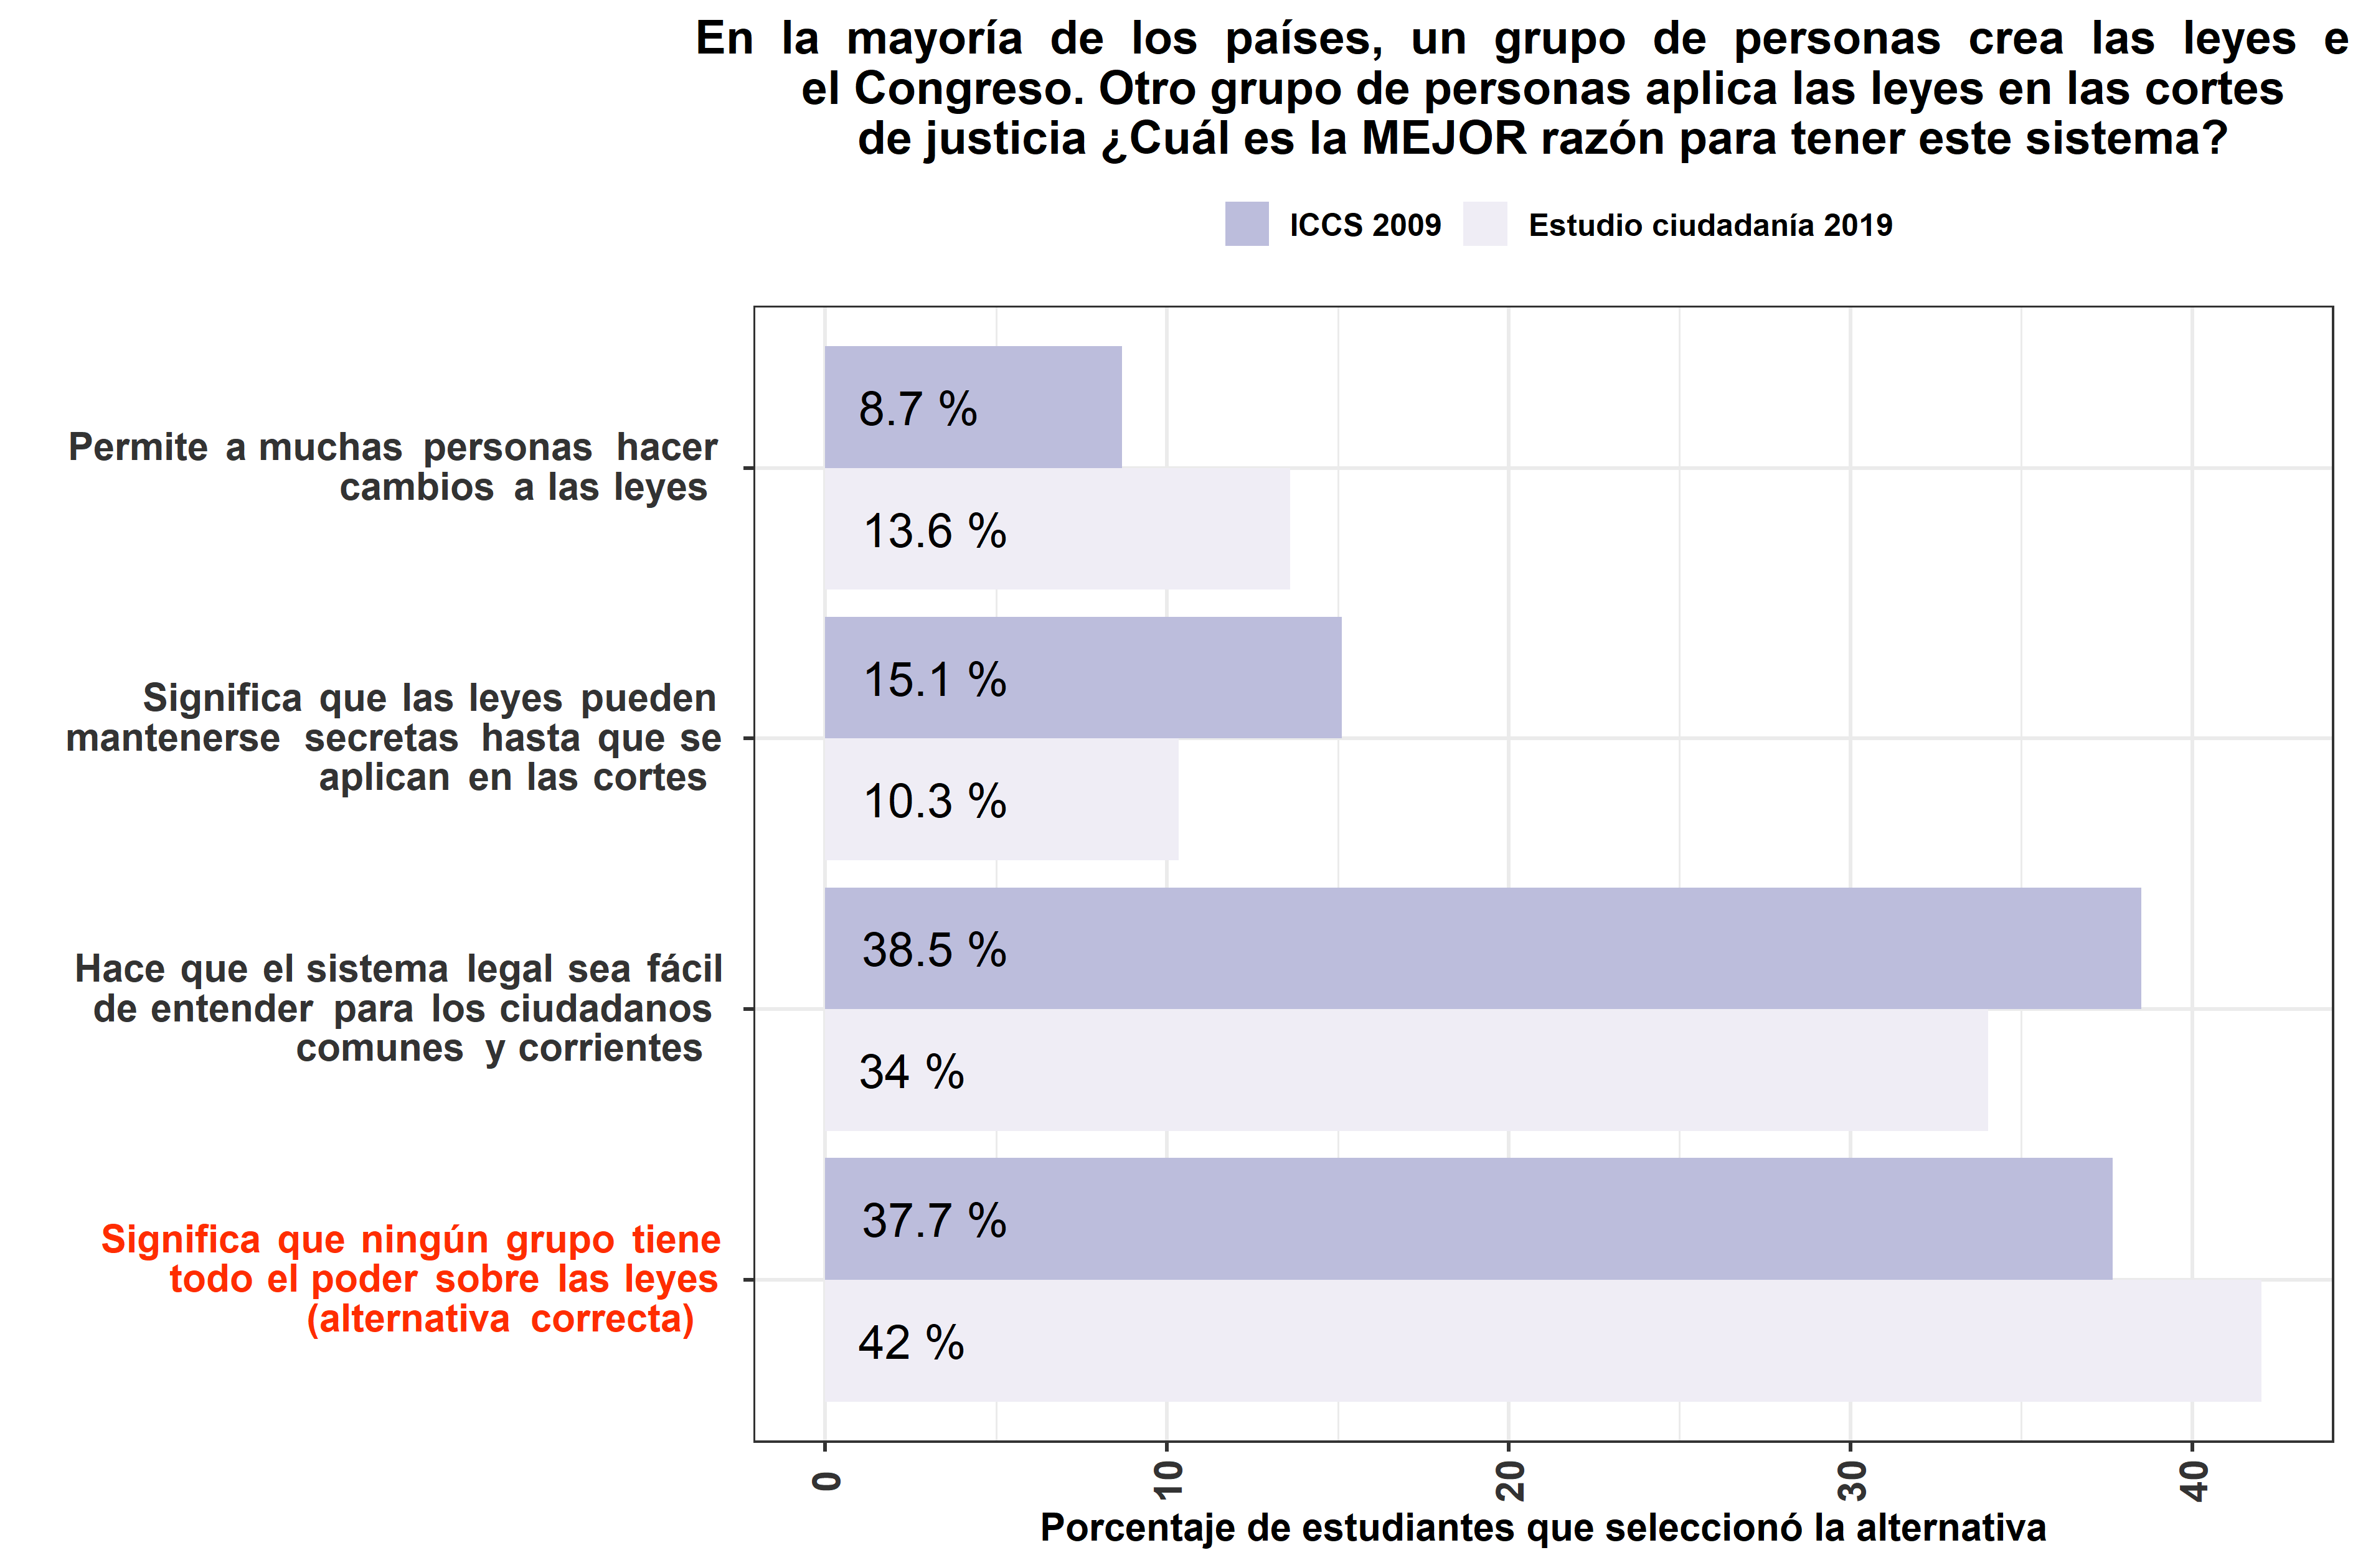
\includegraphics[width=0.8\linewidth,]{images/graph_p1} 

}

\caption{Comparación con ICCS: Razones para crear leyes en el Congreso}\label{fig:unnamed-chunk-19}
\end{figure}

La mayoría de los estudiantes de ambos cursos no respondió de forma correcta la pregunta. La proporción de estudiantes de 2°medio que seleccionó la alternativa correcta es mayor que la proporción de estudiantes de 8°básico que respondió correctamente (43.4\% y 37.7\%, respectivamente). Hubo una alternativa incorrecta en particular que fue un distractor importante para los estudiantes de ambos grupos, concentrando el 38.5\% de las respuestas de los estudiantes de 8°básico y el 33.3\% de las respuestas de los estudiantes de 2°medio.

\begin{center}\rule{0.5\linewidth}{0.5pt}\end{center}

\begin{figure}[!ht]

{\centering 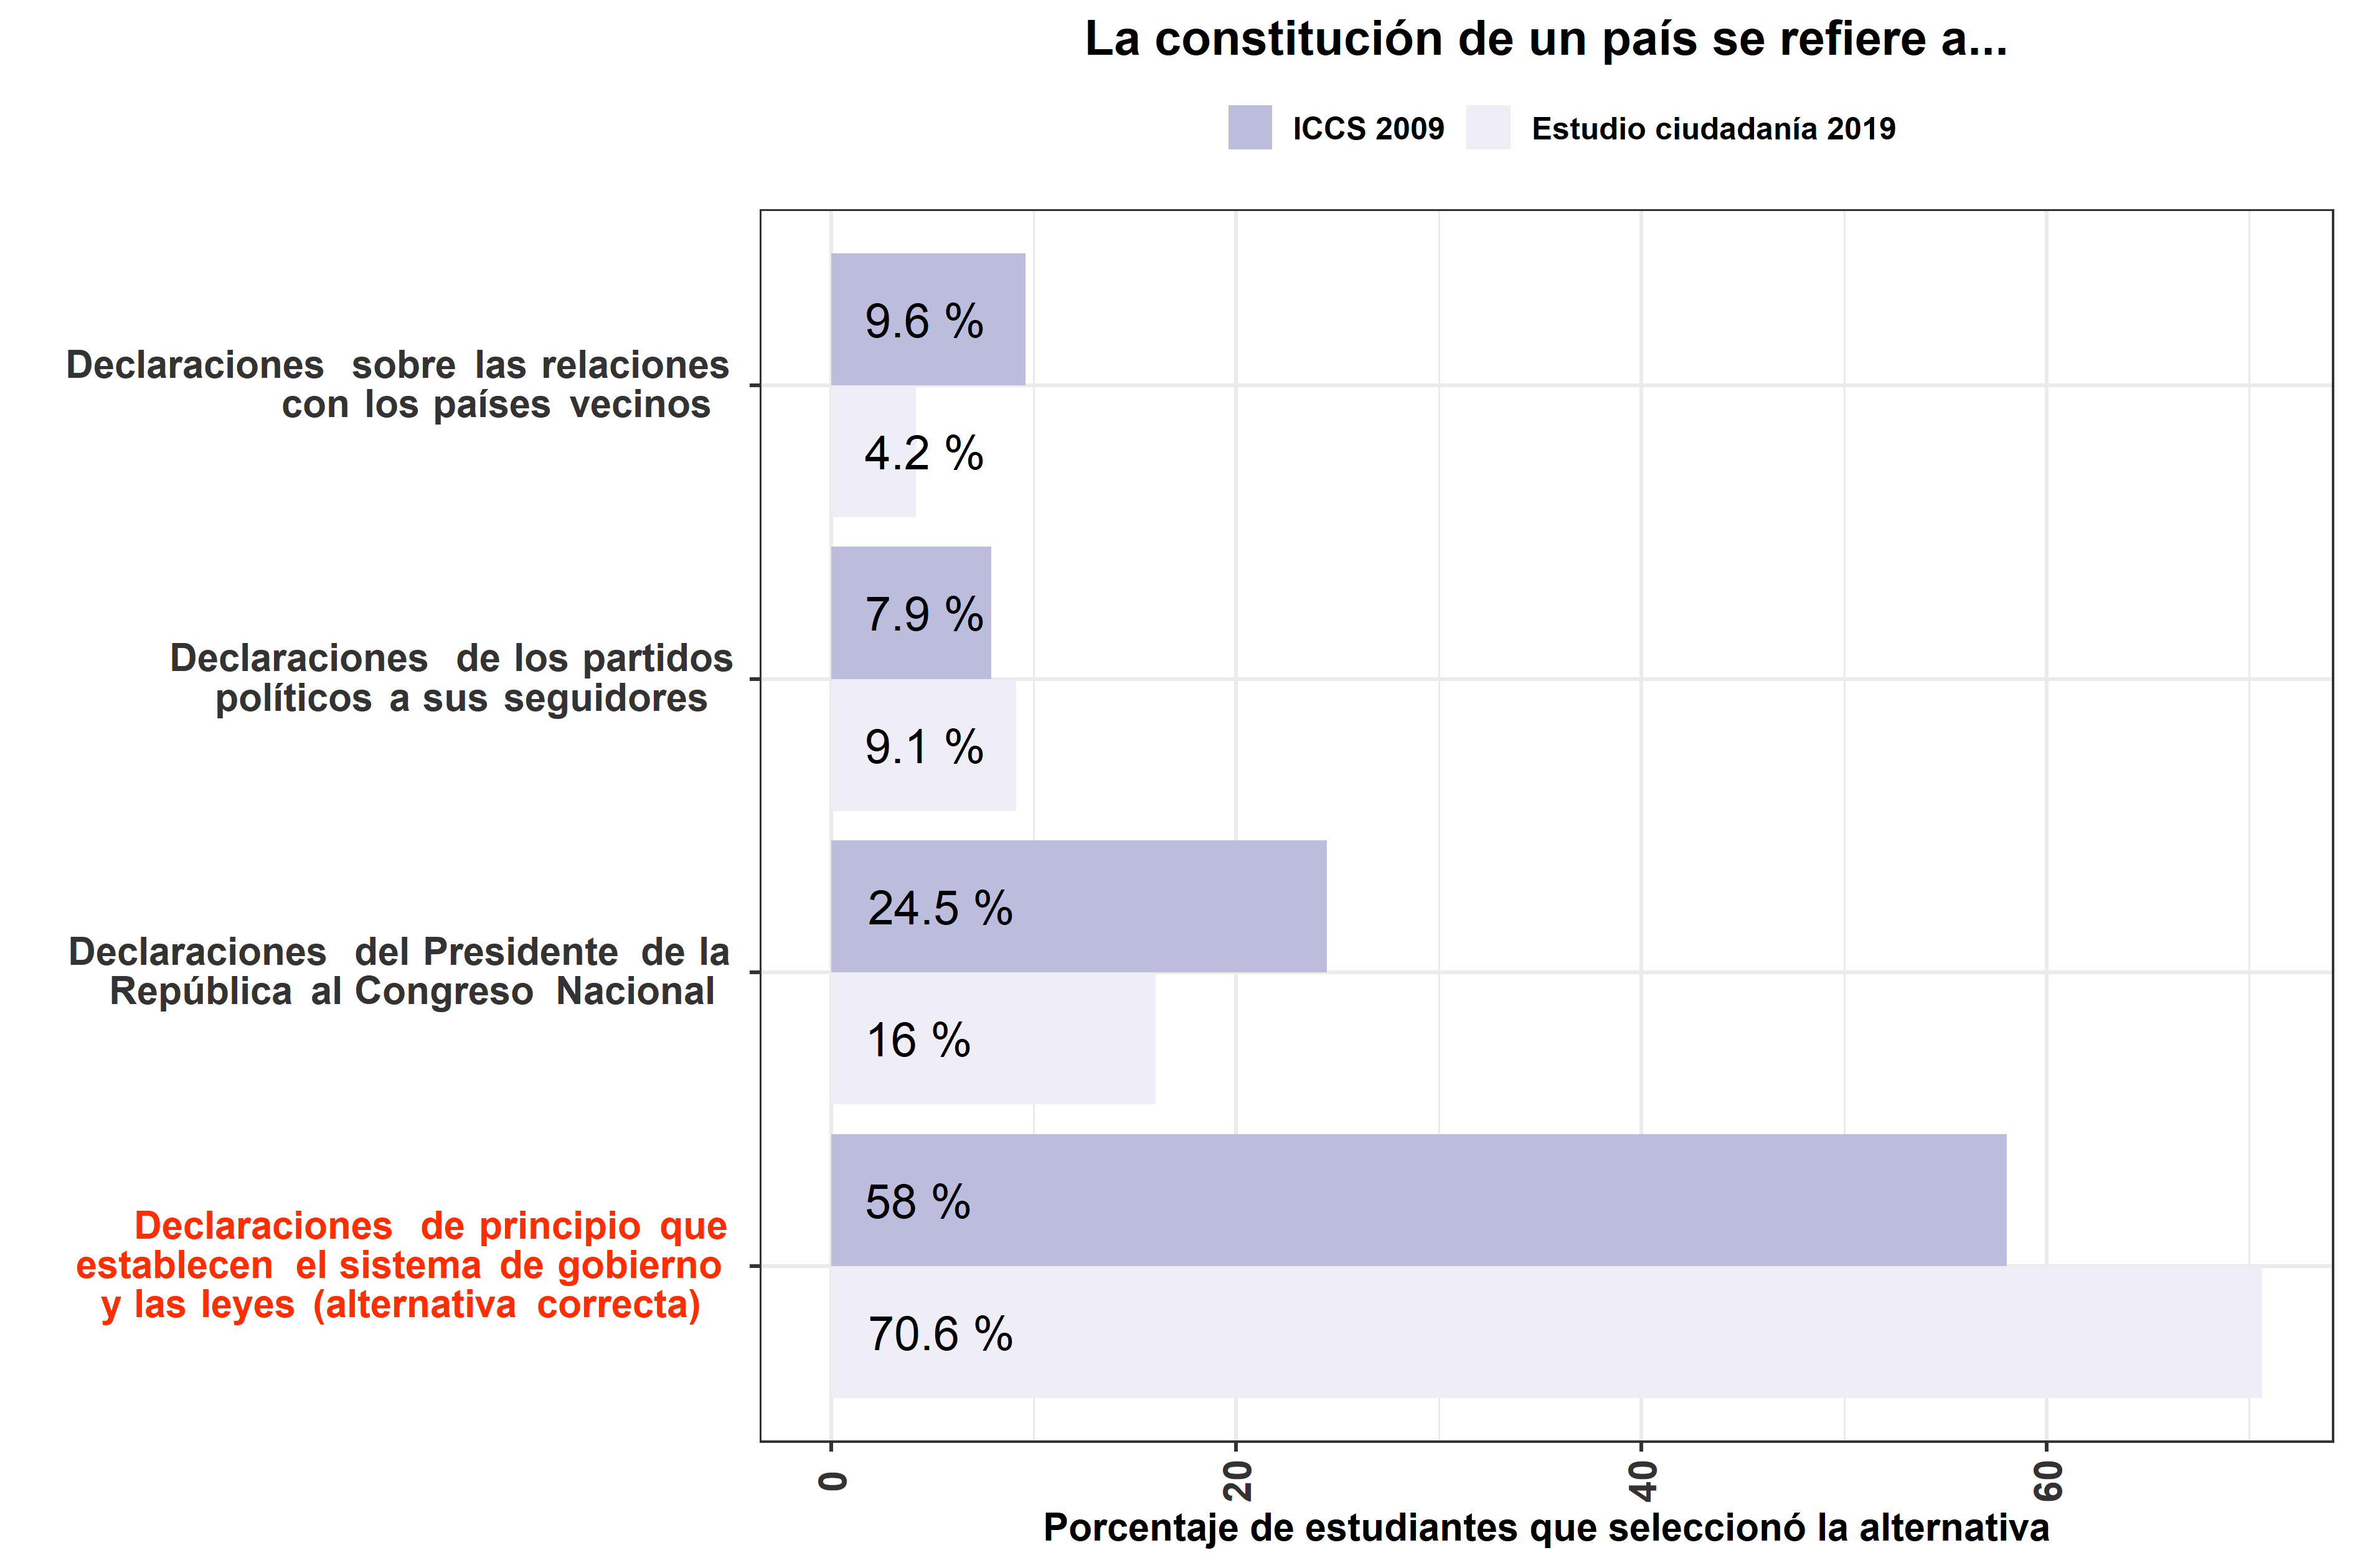
\includegraphics[width=0.8\linewidth,]{images/graph_p2} 

}

\caption{Comparación con ICCS: Definiciones de constitución}\label{fig:unnamed-chunk-20}
\end{figure}

La mayoría de los estudiantes, tanto de 8°básico como de 2°medio, respondió de forma correcta. Sin embargo, la proporción de estudiantes de 2°medio que seleccionó la alternativa correcta es mayor que la proporción de estudiantes de 8°básico que respondió de forma correcta (70.6\% y 58\%, respectivamente). Las respuestas incorrectas de ambos grupos de estudiantes se concentraron en una alternativa en particular. Más específicamente, una de las alternativas incorrectas concentró un 24.5\% de las respuestas de los estudiantes de 8°básico y un 16\% de las respuestas de los estudiantes de 2°medio.

\begin{center}\rule{0.5\linewidth}{0.5pt}\end{center}

\begin{figure}[!ht]

{\centering 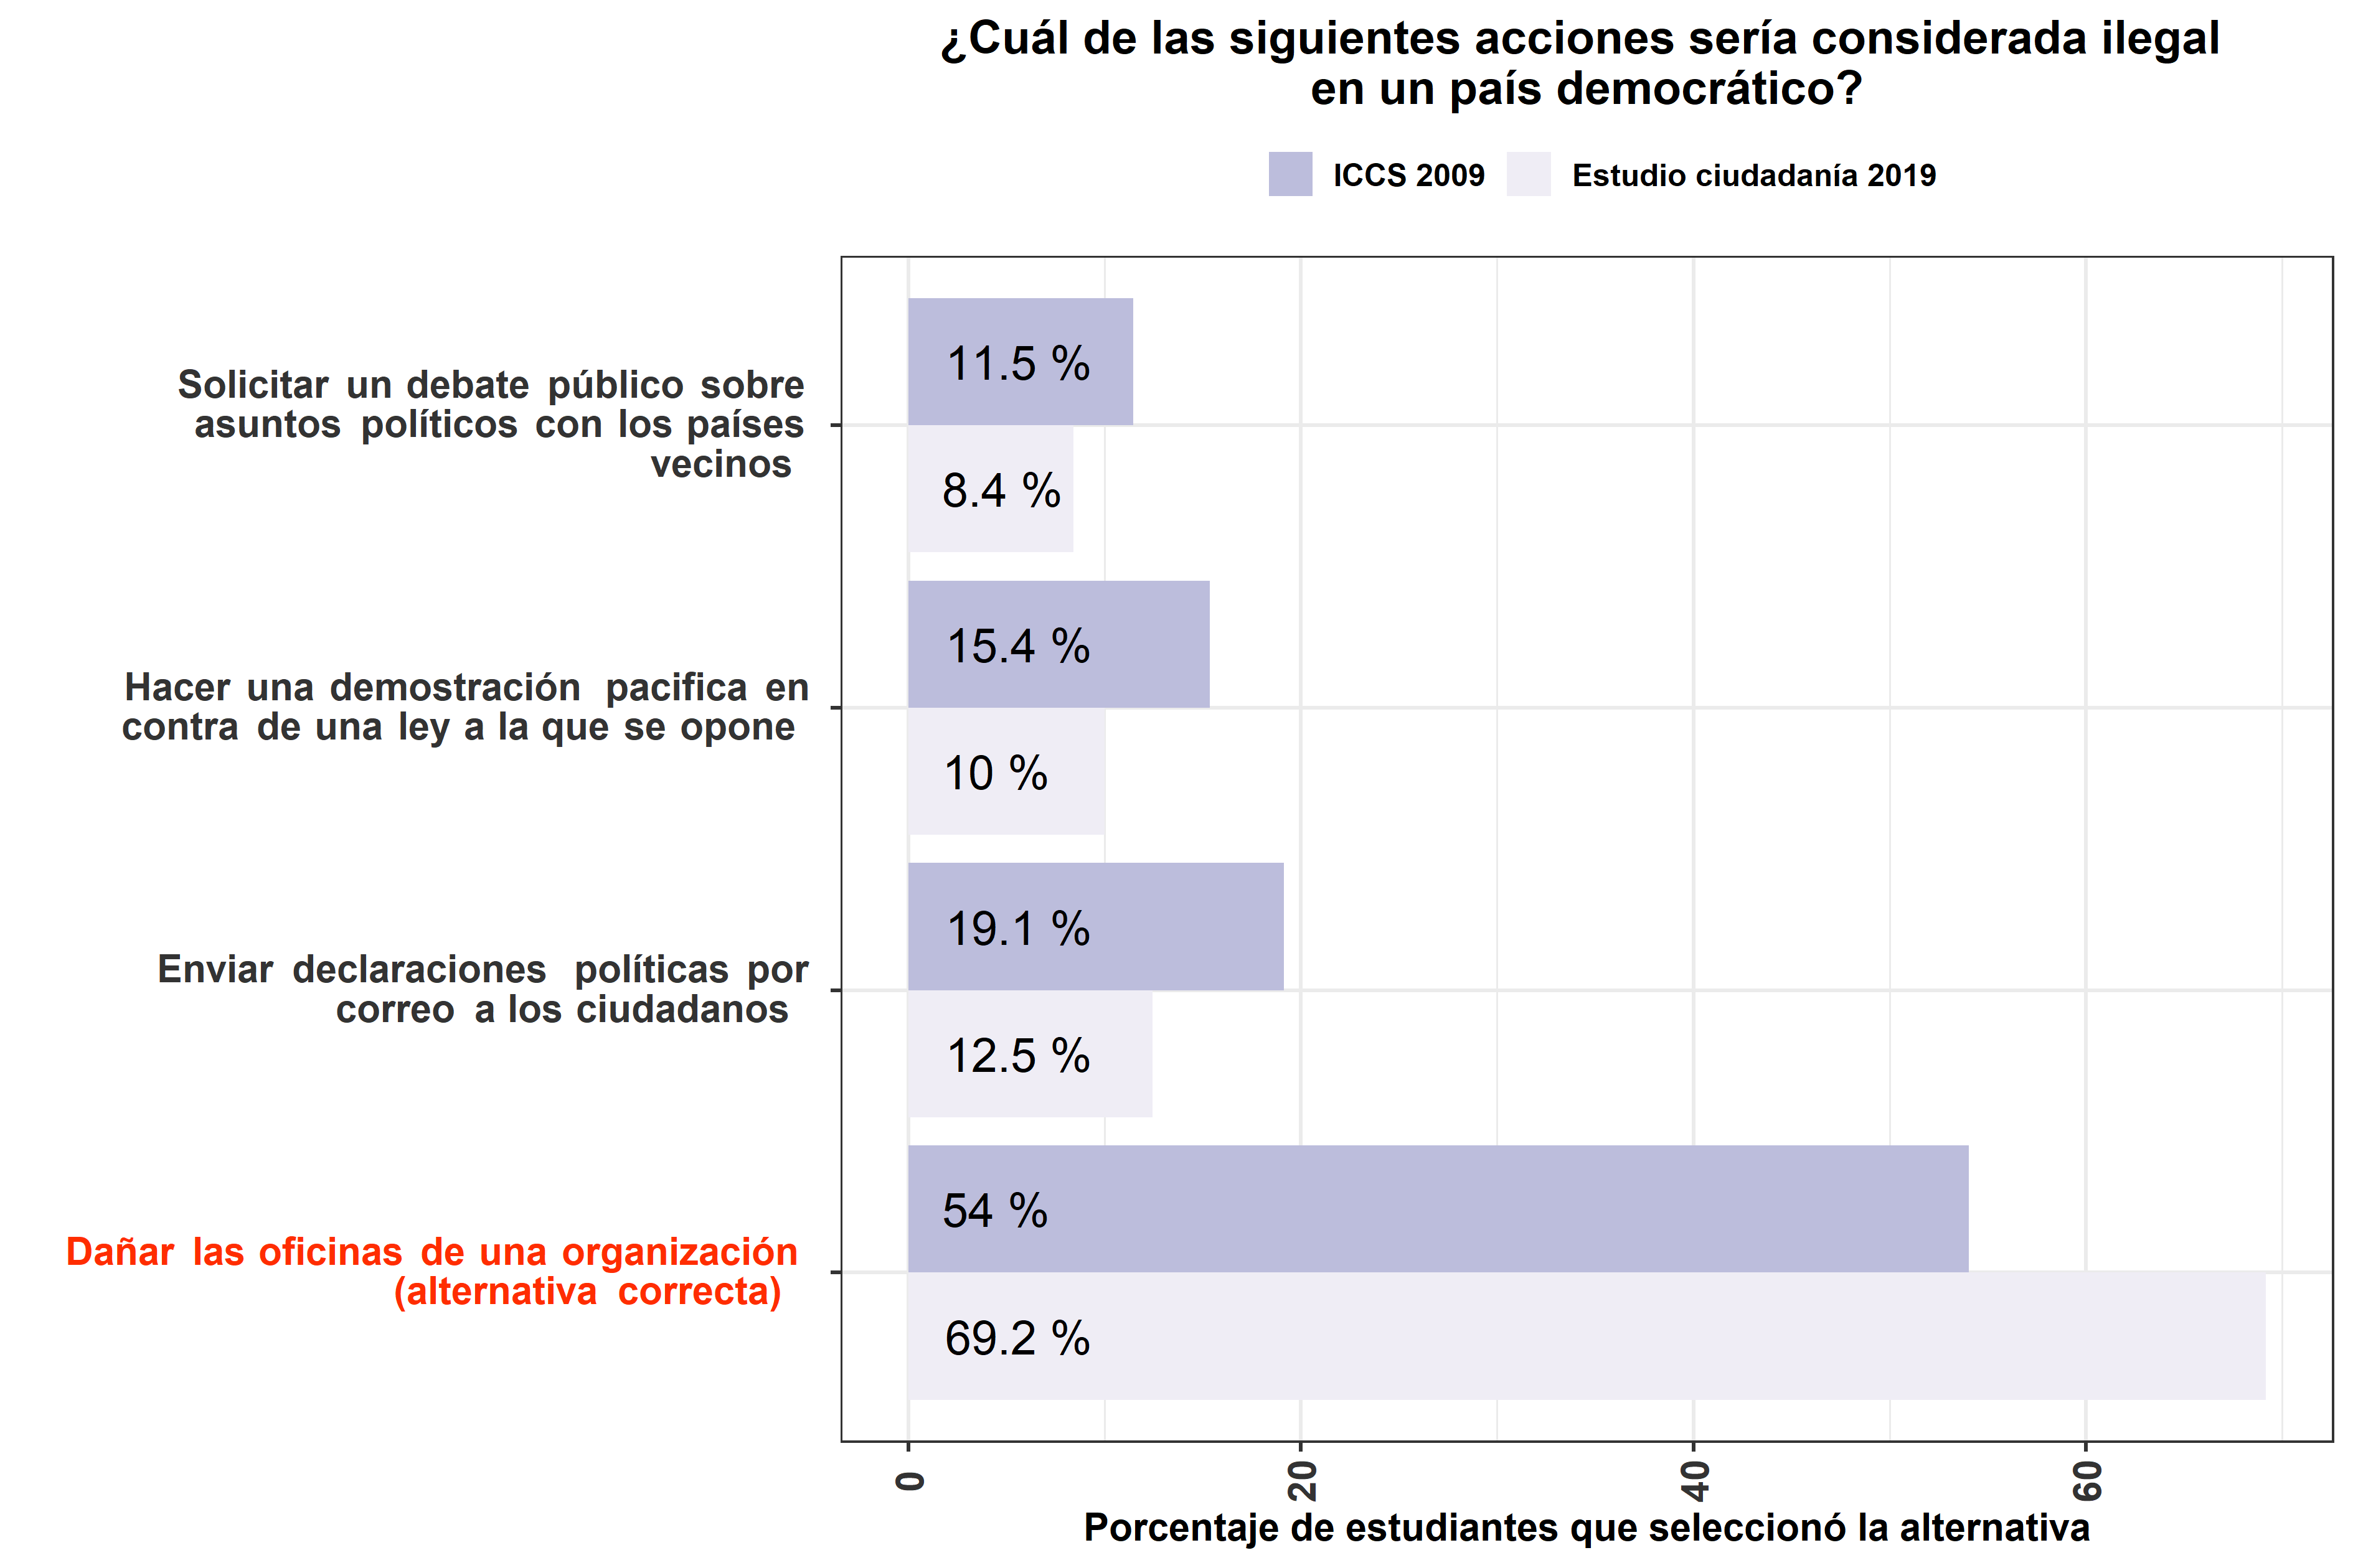
\includegraphics[width=0.8\linewidth,]{images/graph_p3} 

}

\caption{Comparación con ICCS: Acción ilegal en un país democrático}\label{fig:unnamed-chunk-21}
\end{figure}

La mayoría de los estudiantes de ambos grupos respondió de forma correcta, pero la proporción de estudiantes que respondió correctamente es mayor en el grupo de 2°medio que en el de 8°básico (69.2\% y 54\%, respectivamente). En relación con las respuestas incorrectas, cabe destacar que las respuestas de los estudiantes de 2°medio se distribuyeron de forma relativamente pareja entre las distintas alternativas, mientras que las respuestas de los estudiantes de 8°básico se concentraron en una alternativa en particular, la cual fue seleccionada por el 19.1\% de los estudiantes.

\begin{center}\rule{0.5\linewidth}{0.5pt}\end{center}

\begin{figure}[!ht]

{\centering 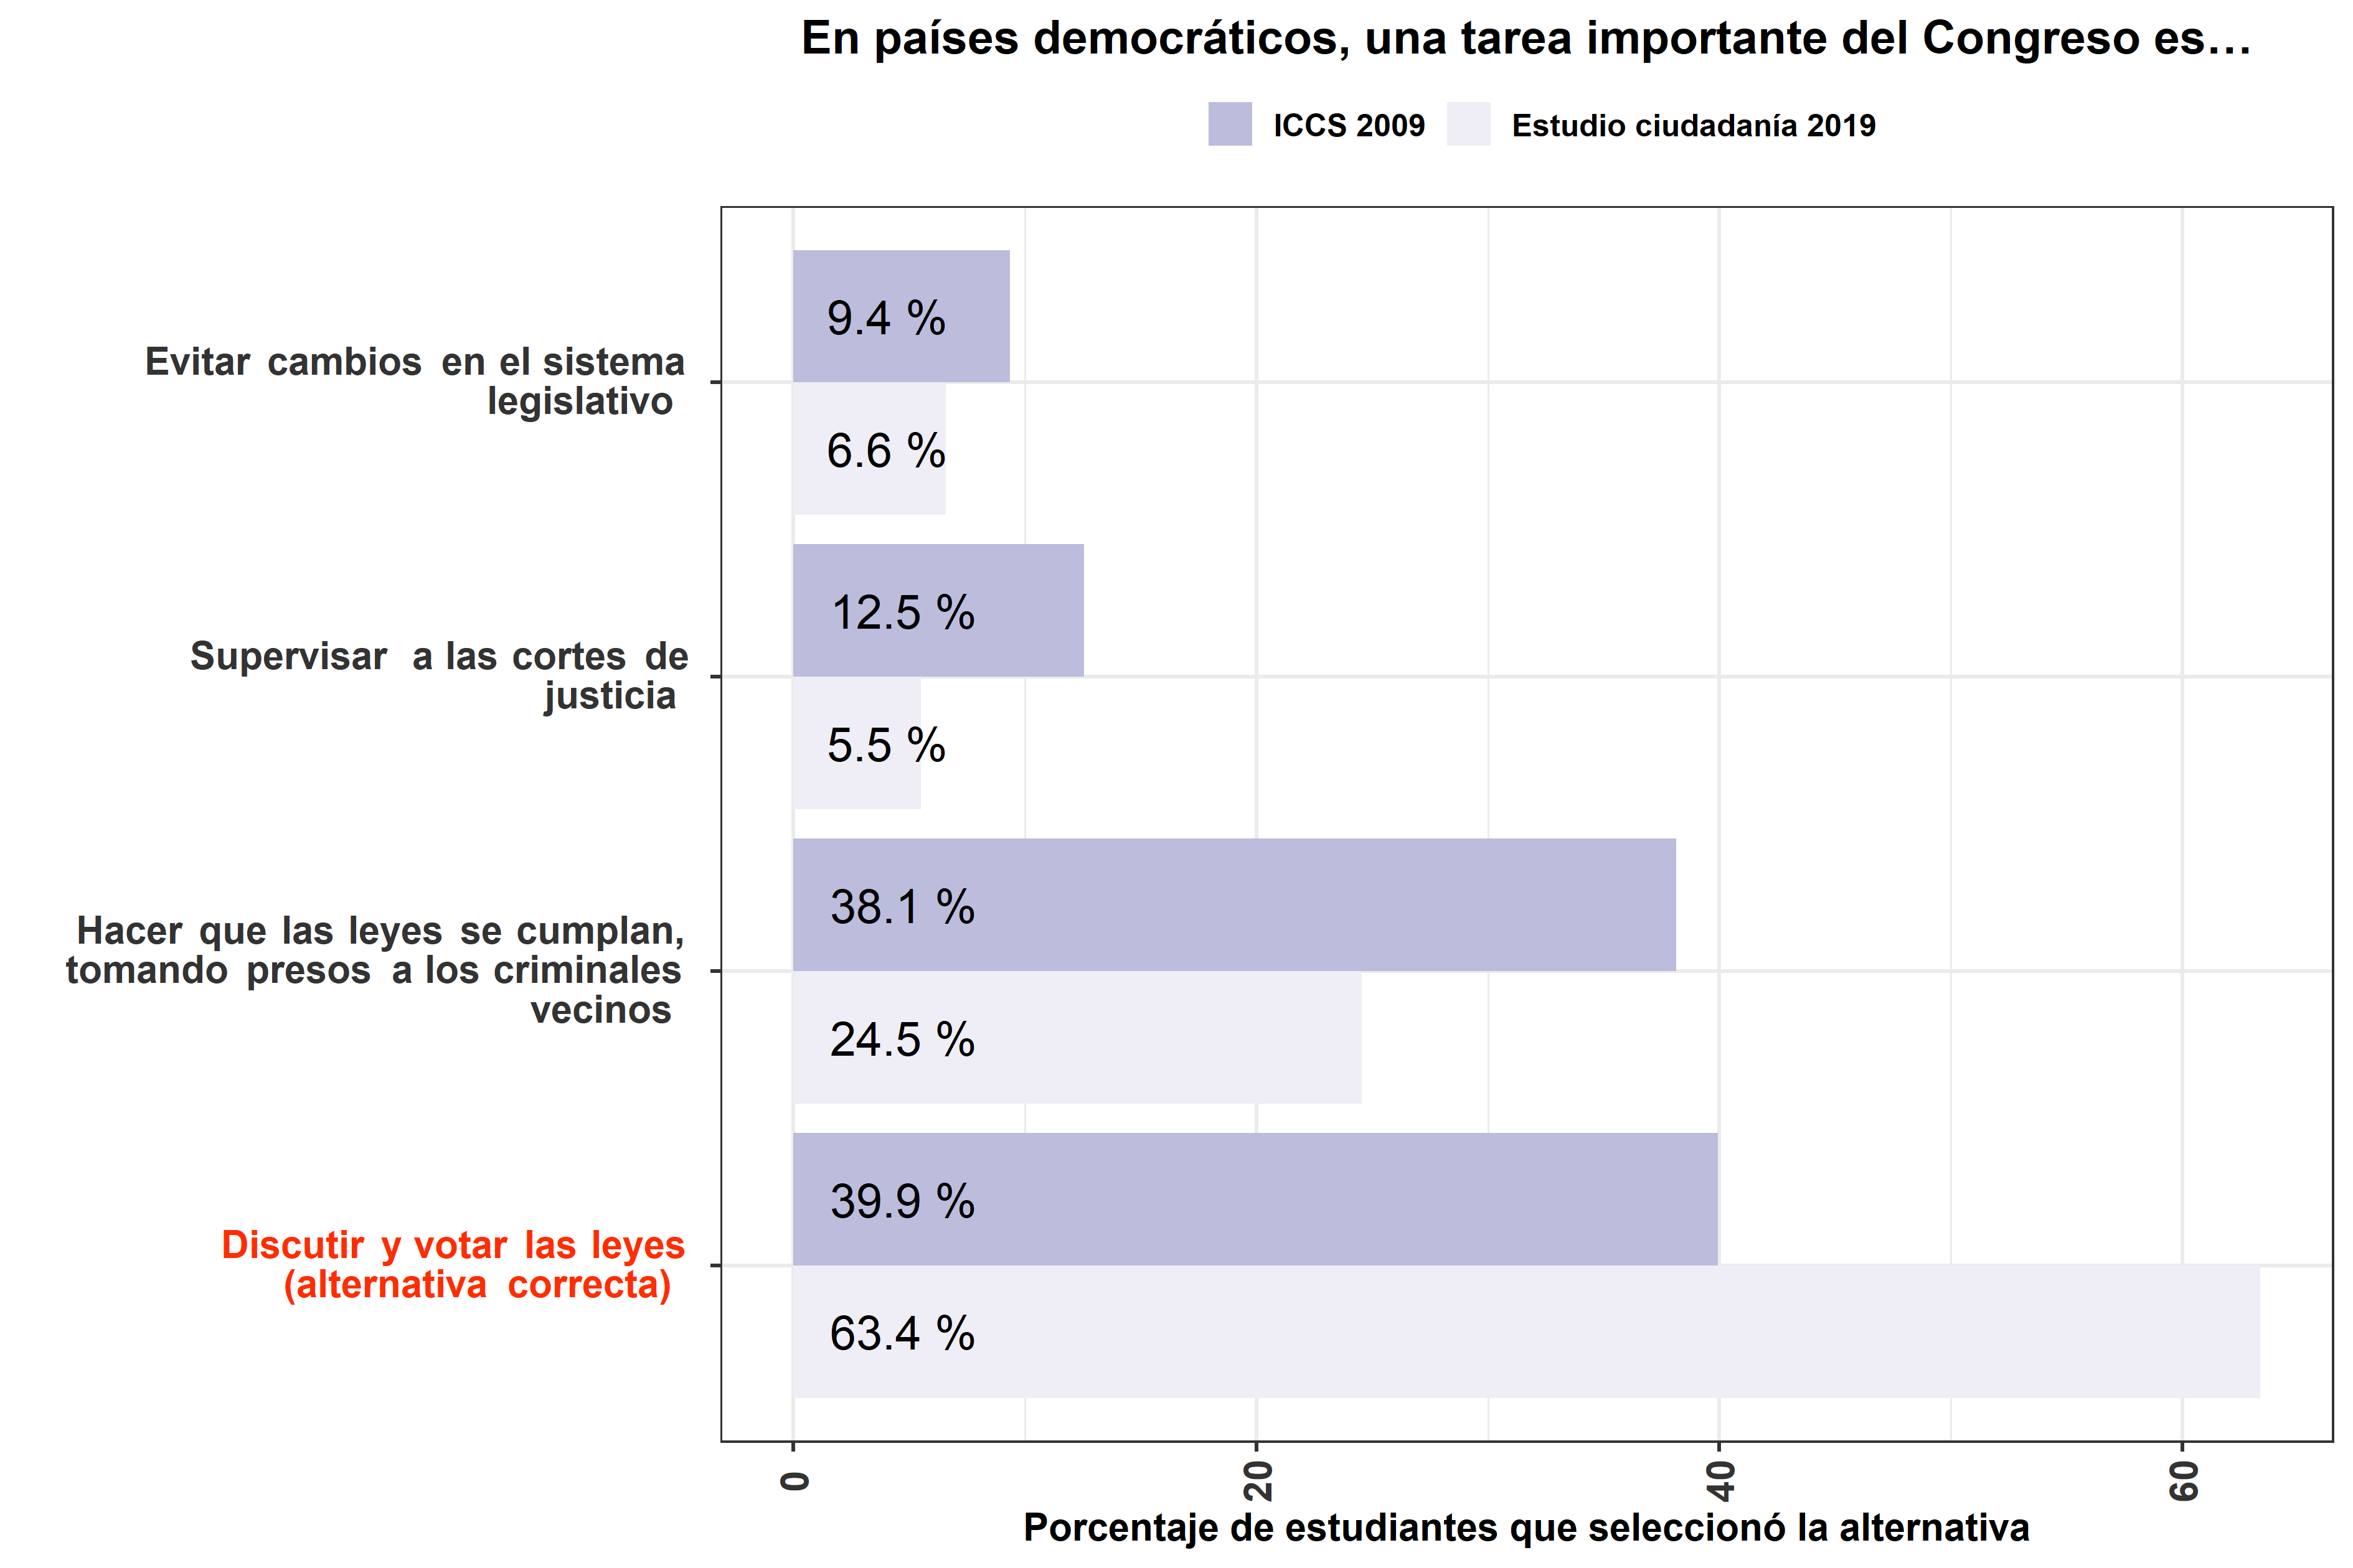
\includegraphics[width=0.8\linewidth,]{images/graph_p4} 

}

\caption{Comparación con ICCS: Actividad principal del Congreso}\label{fig:unnamed-chunk-22}
\end{figure}

La mayoría de los estudiantes de 2°medio (un 63.4\%) respondió de forma correcta, mientras que la mayoría de los estudiantes de 8°básico respondió de forma incorrecta. La alternativa que fue seleccionada por una proporción mayor de estudiantes (en ambos grupos) corresponde a la alternativa correcta. Sin embargo, la proporción de estudiantes de 8°básico que identificó la respuesta correcta es mucho menor a la proporción de estudiantes de 2°medio que respondió correctamente (39.9\% y 63.4\%, respectivamente). Una de las alternativas incorrectas concentró parte importante de las respuestas restantes, siendo seleccionada por el 38.1\% de los estudiantes de 8°básico y por el 24.5\% de los estudiantes de 2°medio.

\begin{center}\rule{0.5\linewidth}{0.5pt}\end{center}

\begin{figure}[!ht]

{\centering 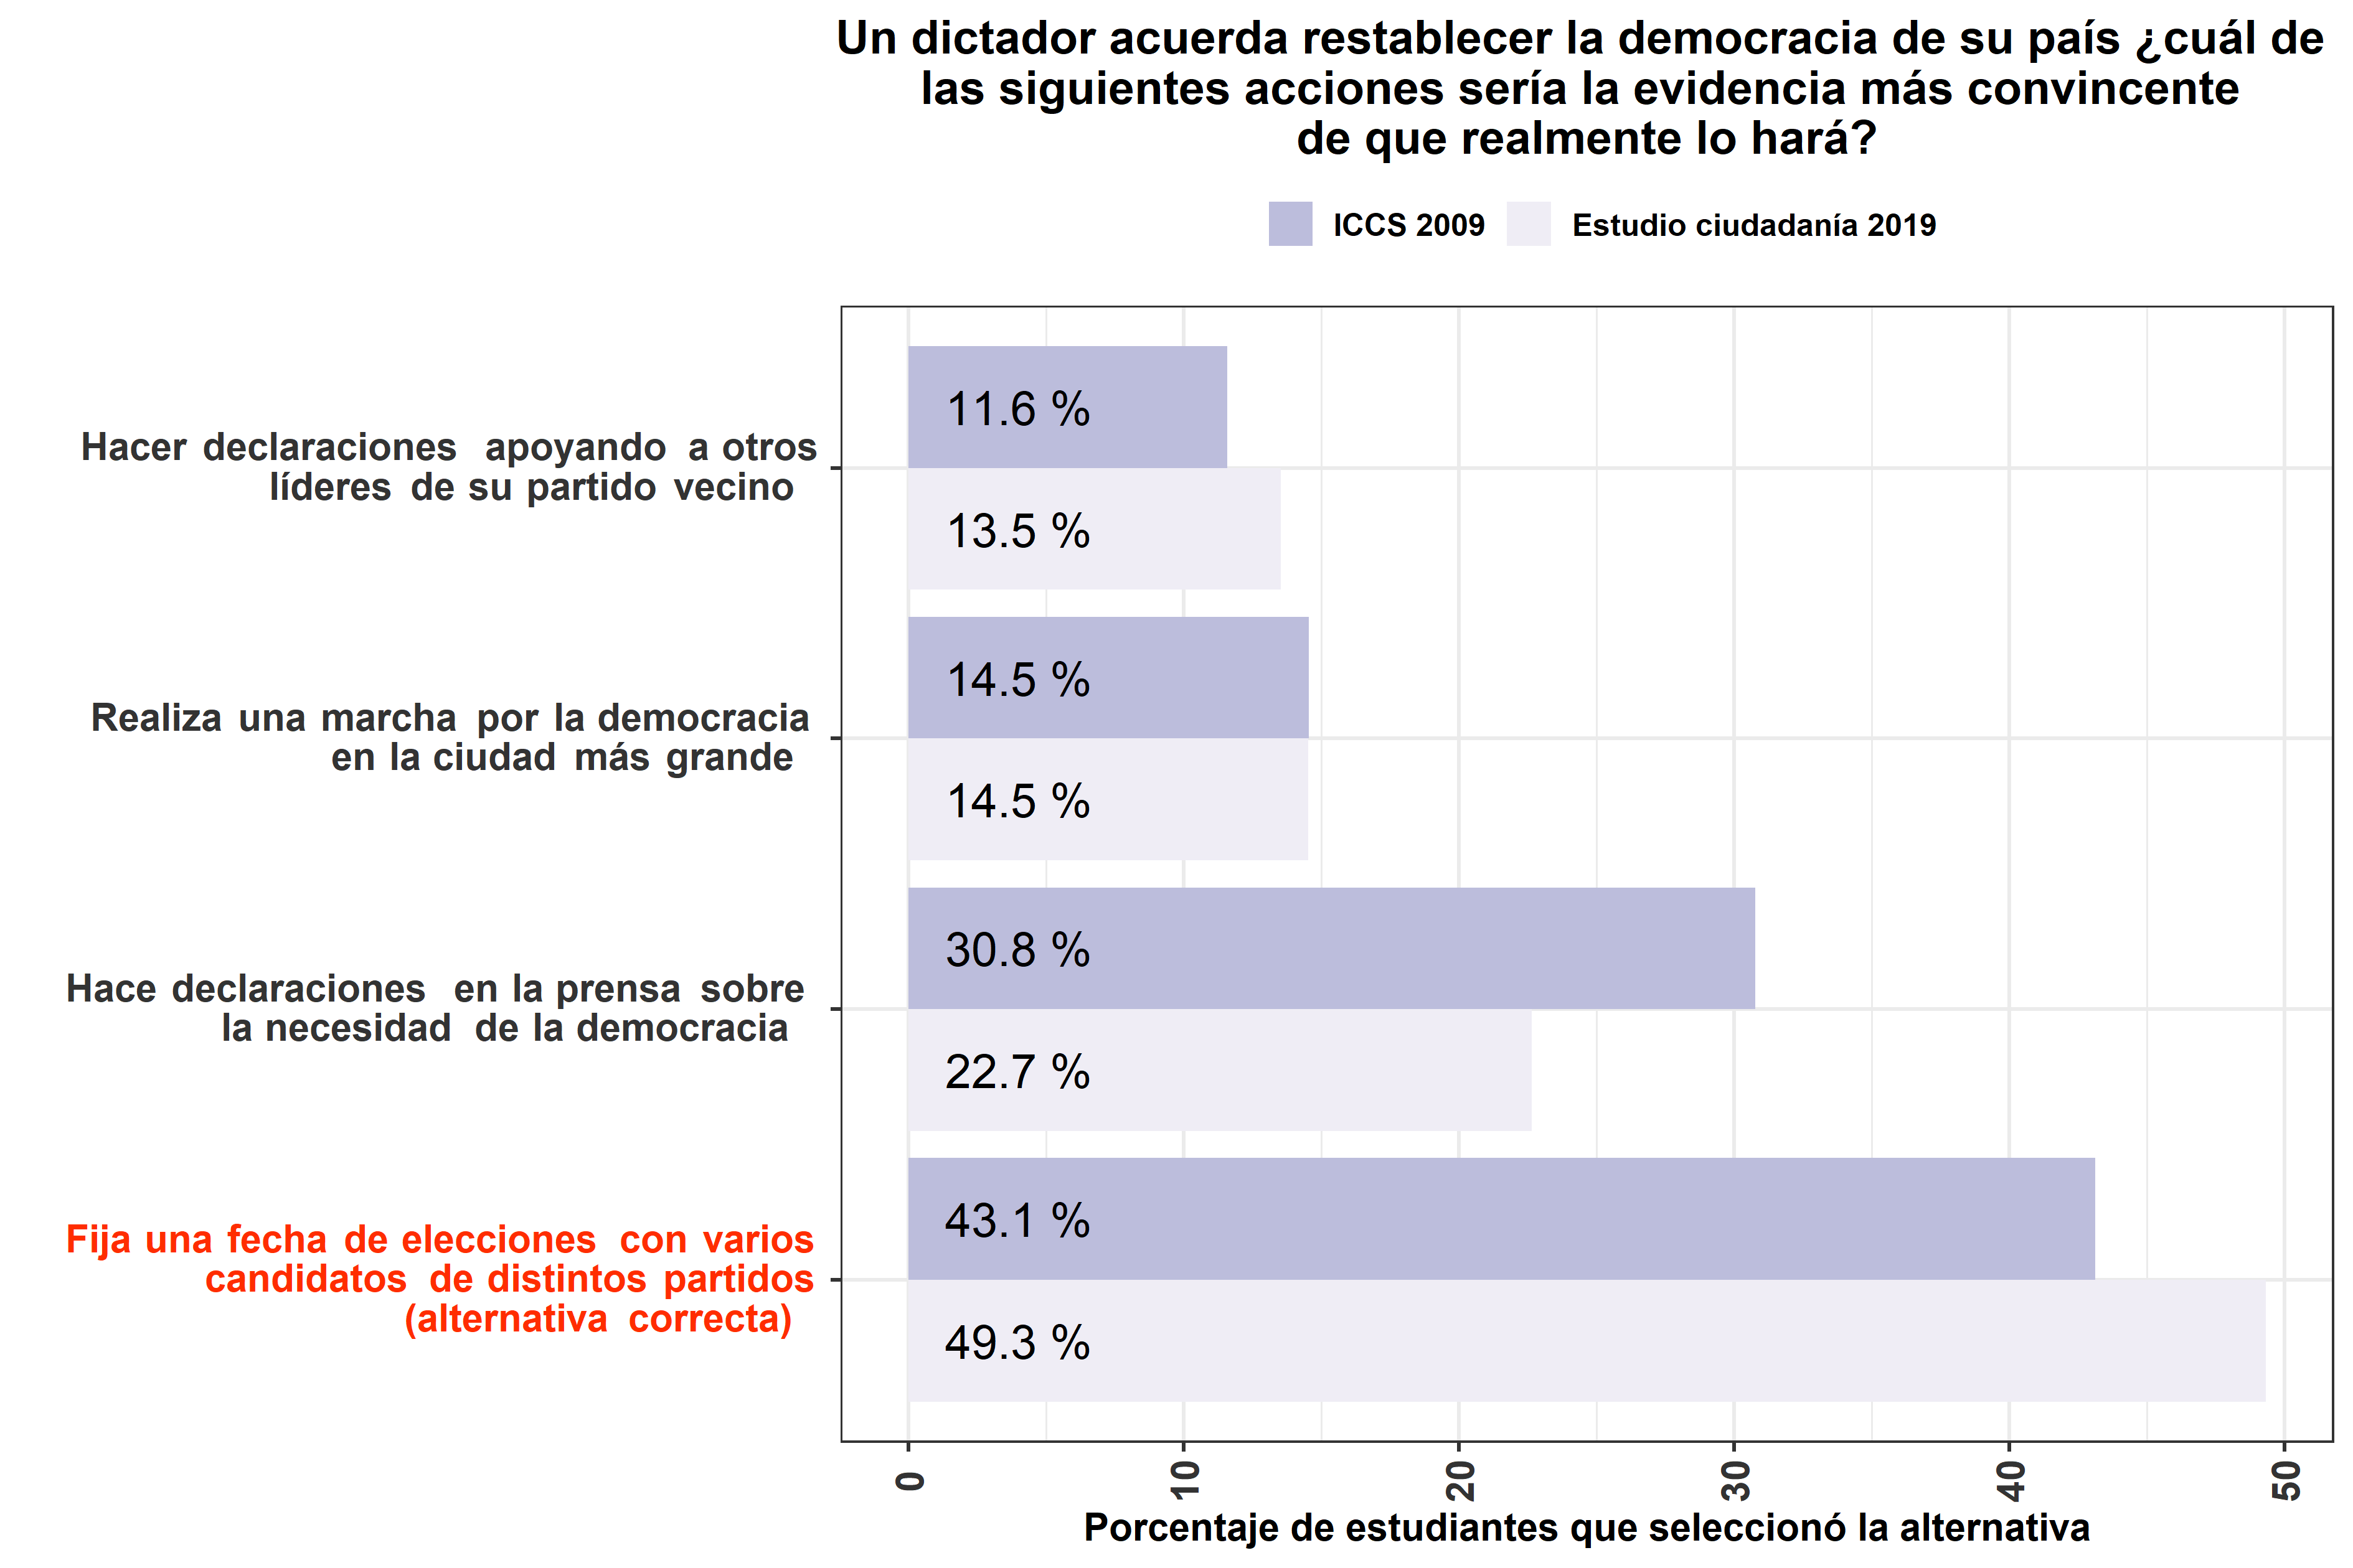
\includegraphics[width=0.8\linewidth,]{images/graph_p5} 

}

\caption{Comparación con ICCS: Acción que demuestra que un dictador restablecerá la democracia}\label{fig:unnamed-chunk-23}
\end{figure}

La mayoría de los estudiantes de 8°básico respondió de forma incorrecta y la mayoría de los estudiantes de 2°medio respondió de manera correcta. Más precisamente, un 43.1\% de los estudiantes de 8°básico y un 50.7\% de los estudiantes de 2°medio seleccionaron la alternativa correcta. Las respuestas incorrectas de ambos grupos de estudiantes se concentraron en una alternativa en particular, la cual fue seleccionada por el 30.8\% de los estudiantes de 8°básico y el 24\% de los estudiantes de 2°medio.

\begin{center}\rule{0.5\linewidth}{0.5pt}\end{center}

\begin{figure}[!ht]

{\centering 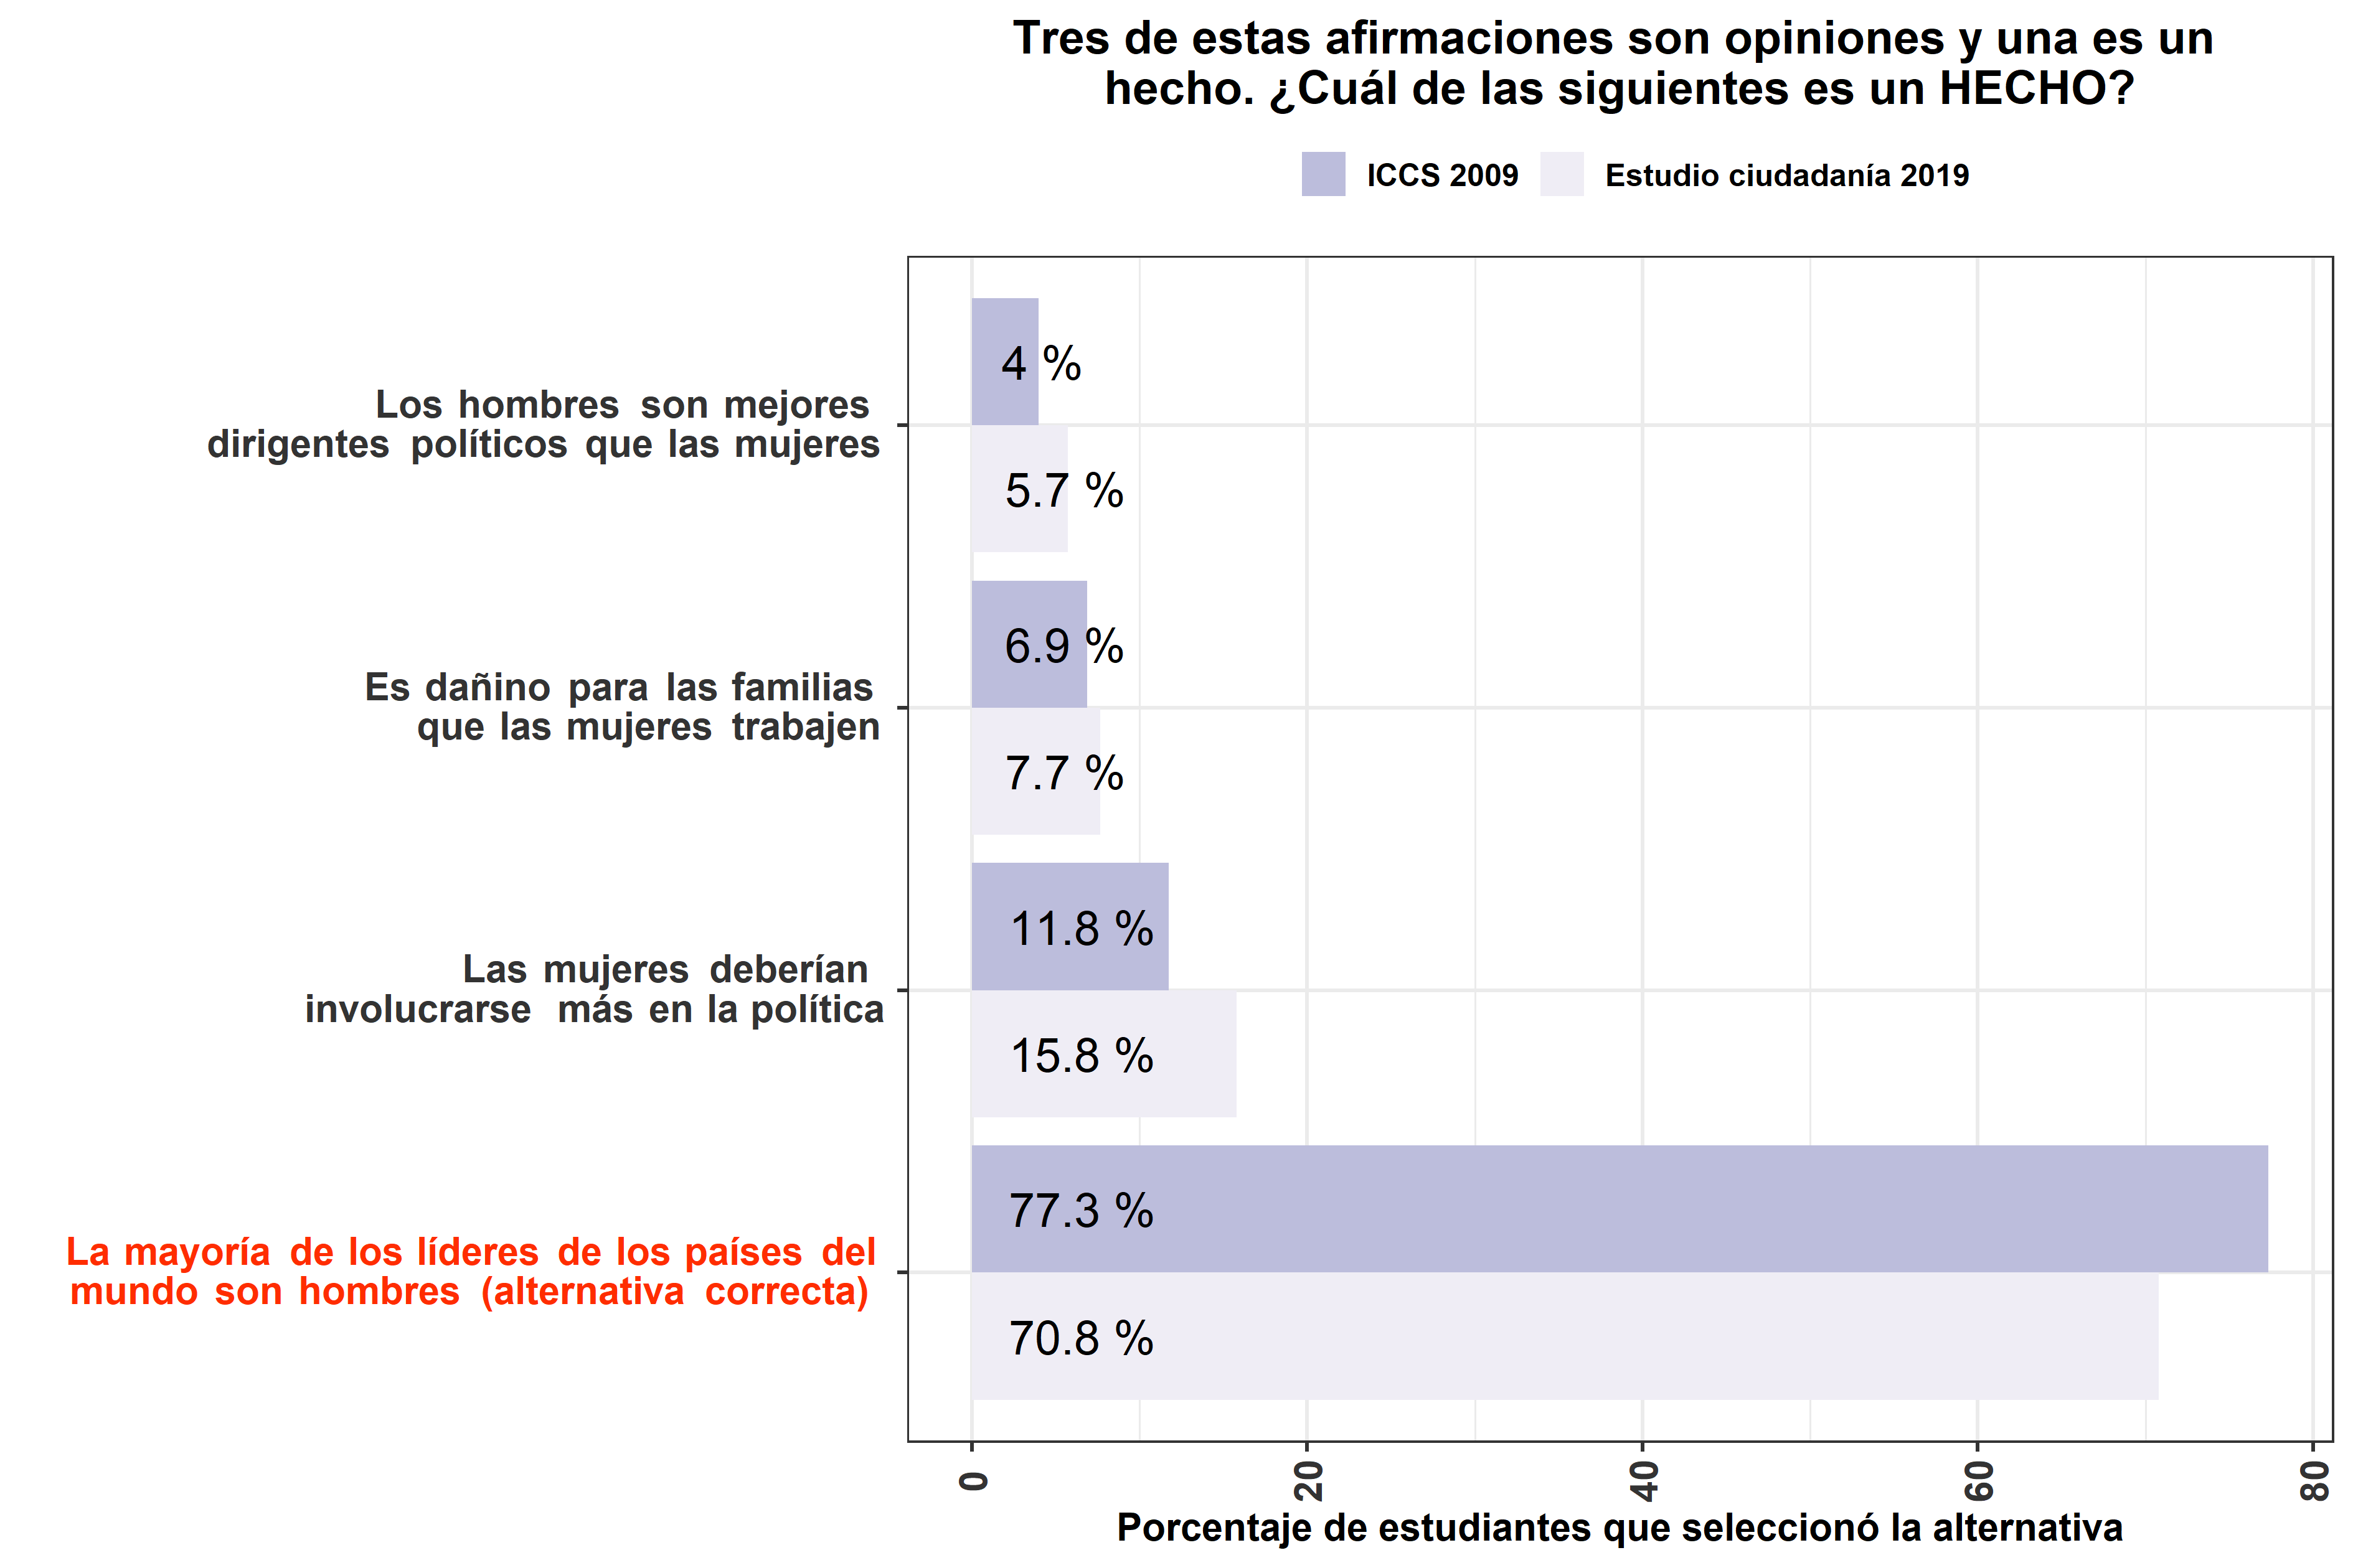
\includegraphics[width=0.8\linewidth,]{images/graph_p6} 

}

\caption{Comparación con ICCS: Afirmación que corresponde a un hecho}\label{fig:unnamed-chunk-24}
\end{figure}

La mayoría de los estudiantes seleccionó la alternativa correcta. A diferencia de las respuestas en las otras preguntas, la proporción de estudiantes de 8°básico que identificó la respuesta correcta fue un poco mayor a la proporción de estudiantes de 2°medio que respondió correctamente. Más específicamente, un 77.3\% de los estudiantes de 8°básico y un 75.2\% de los estudiantes de 2°medio seleccionaron la alternativa correcta. Las respuestas incorrectas de los estudiantes de ambos grupos se concentraron en una alternativa en particular, que fue seleccionada por el 11.8\% de los estudiantes de 8°básico y el 14.2\% de los estudiantes de 2°medio.

\begin{center}\rule{0.5\linewidth}{0.5pt}\end{center}

\hypertarget{buena-ciudadanuxeda}{%
\section{Buena ciudadanía}\label{buena-ciudadanuxeda}}

En esta sección se presentarán los resultados de una serie de preguntas referidas a la formación ciudadana de los estudiantes. En el análisis de estas preguntas se compararan las respuestas de los docentes, los estudiantes y los apoderados.

\hypertarget{importancia-de-distintos-aspectos-en-la-formaciuxf3n-ciudadana}{%
\subsection{Importancia de distintos aspectos en la formación ciudadana}\label{importancia-de-distintos-aspectos-en-la-formaciuxf3n-ciudadana}}

\begin{center}\rule{0.5\linewidth}{0.5pt}\end{center}

\begin{figure}[!ht]

{\centering 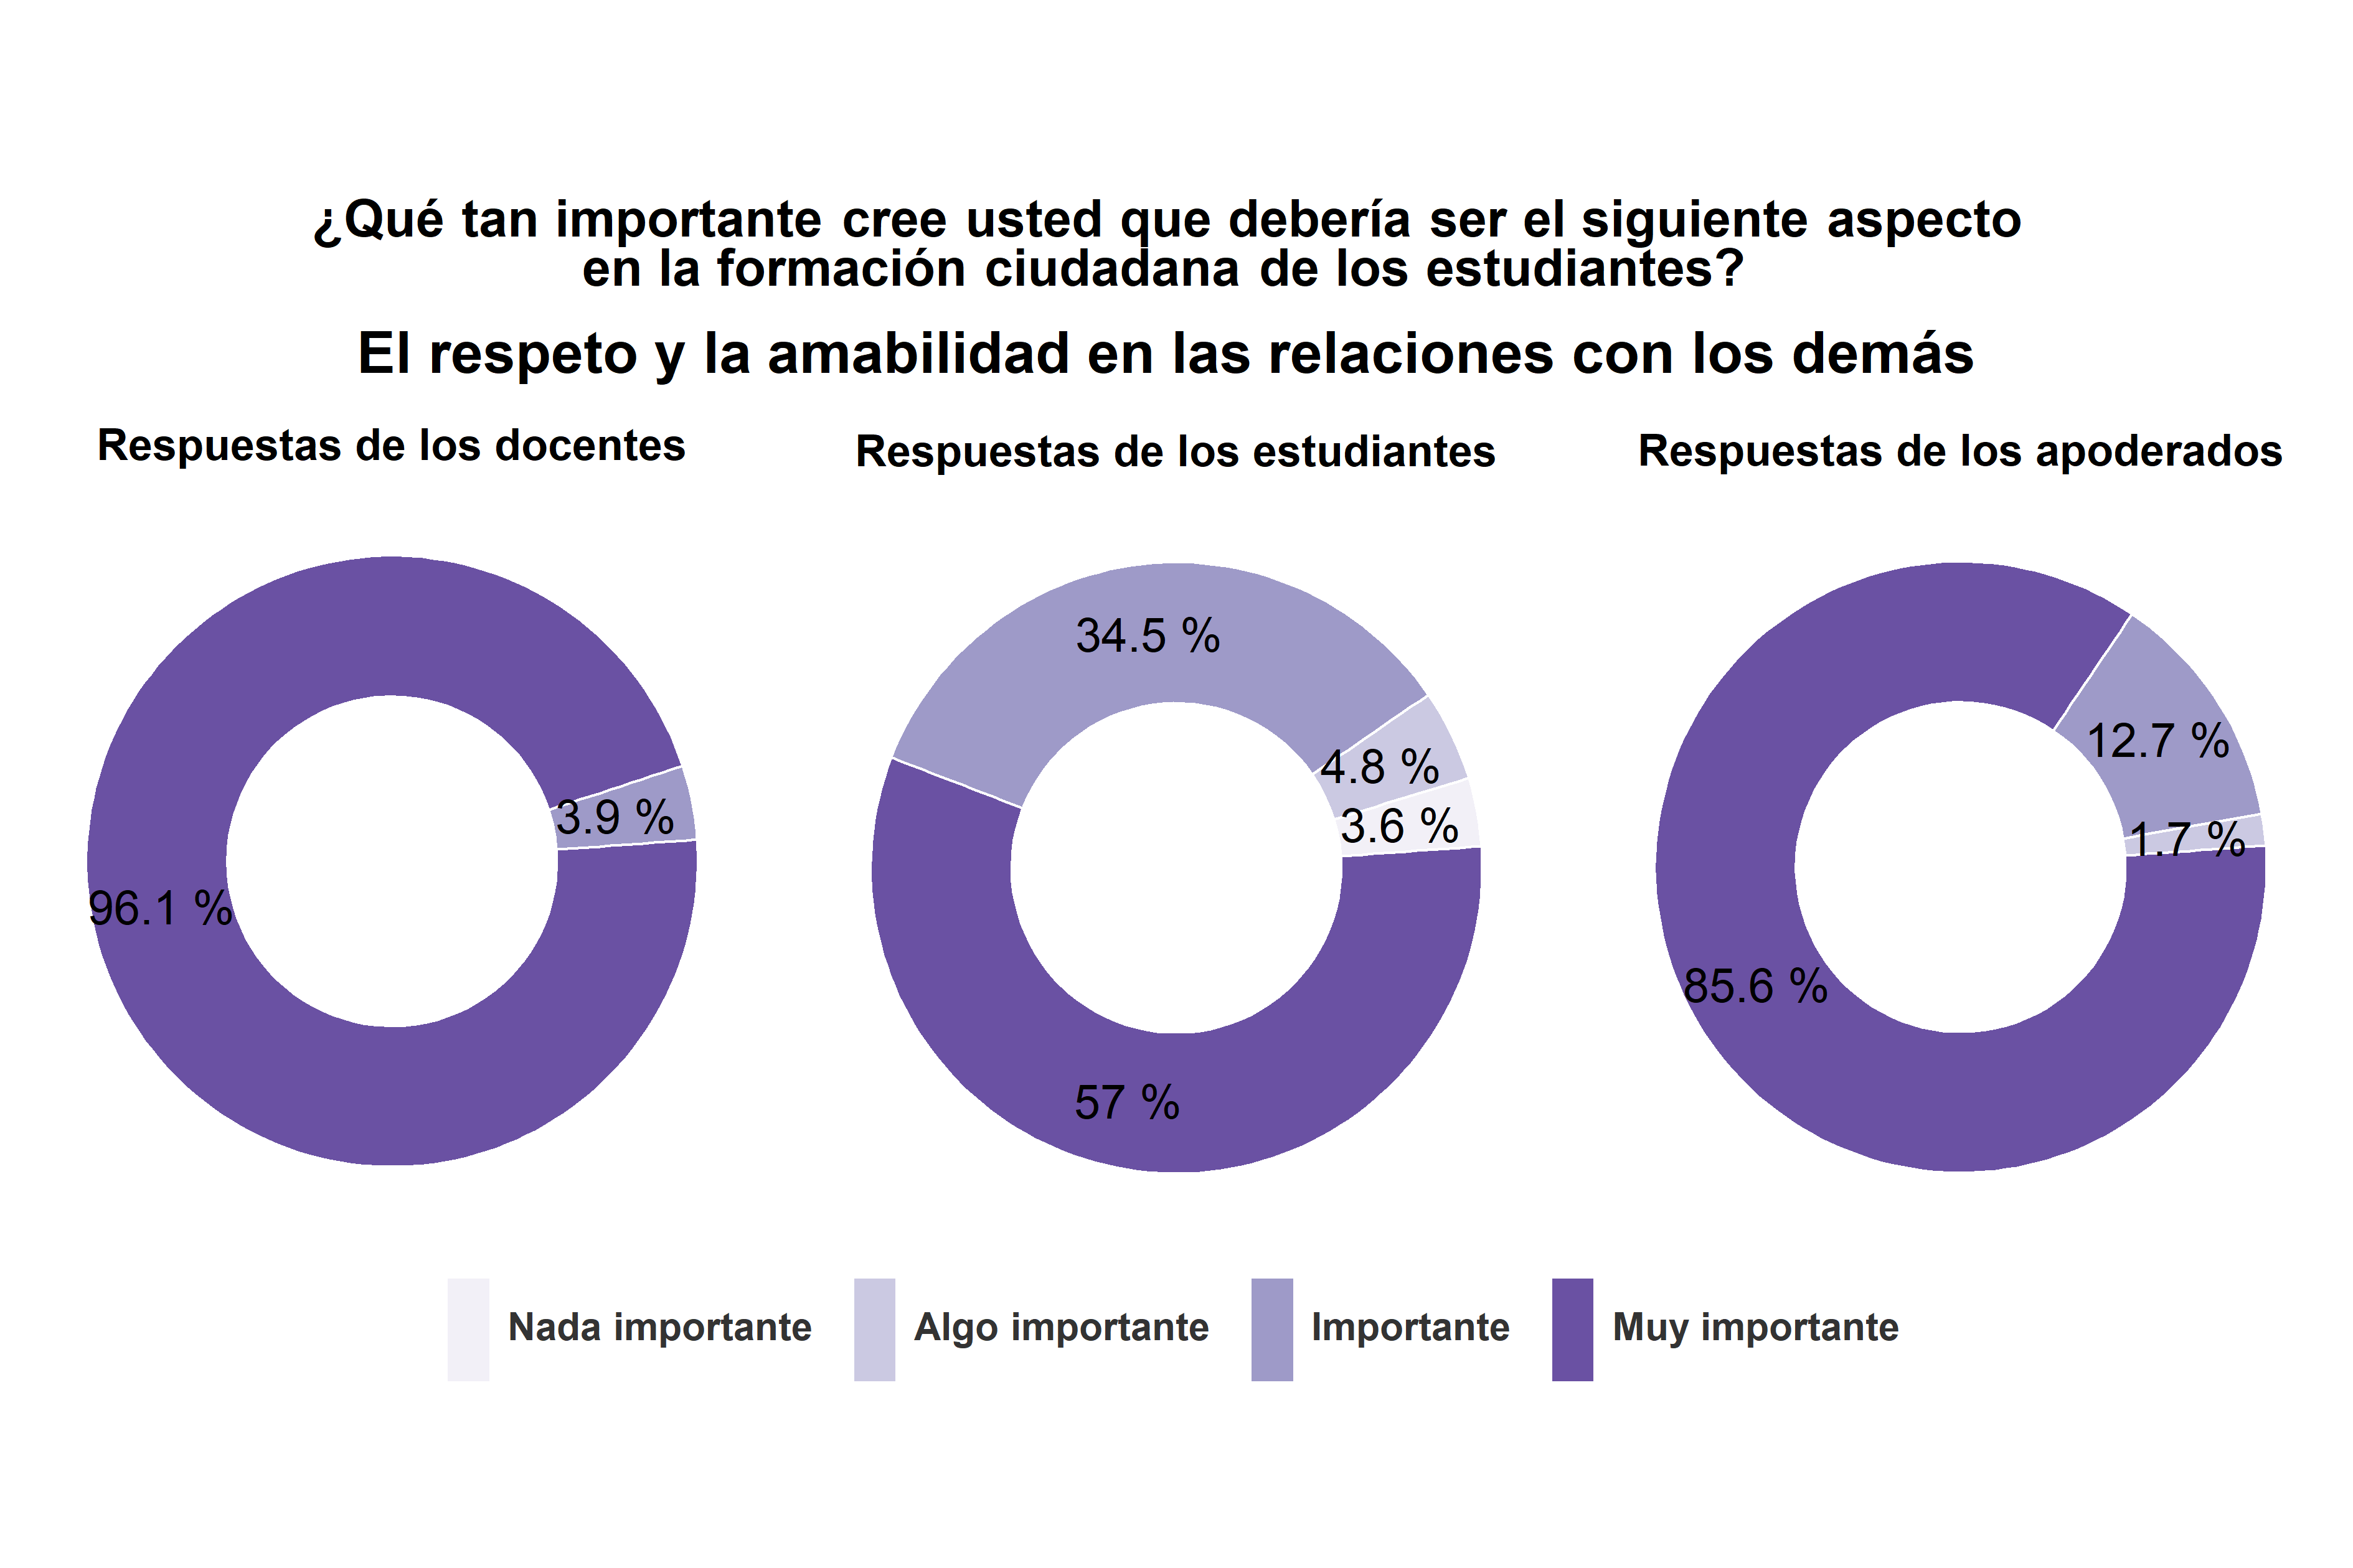
\includegraphics[width=0.8\linewidth,]{images/graph_for_ciud1} 

}

\caption{Relevancia del respeto en las relaciones con los demás}\label{fig:unnamed-chunk-25}
\end{figure}

La mayoría de los docentes, estudiantes y apoderados cree que \emph{el respeto y la amabilidad en las relaciones con los demás} son un aspecto muy importante en la formación ciudadana de los estudiantes. Más específicamente, el 94.9\% de los docentes, el 61.6\% de los estudiantes y el 86.3\% de los apoderados creen que es muy importante. En relación a las alternativas nada importante y algo importante cabe destacar que ninguno de los docentes optó por esas respuestas y que ninguno de los apoderados declaró que es un aspecto nada importante.

\begin{center}\rule{0.5\linewidth}{0.5pt}\end{center}

\begin{figure}[!ht]

{\centering 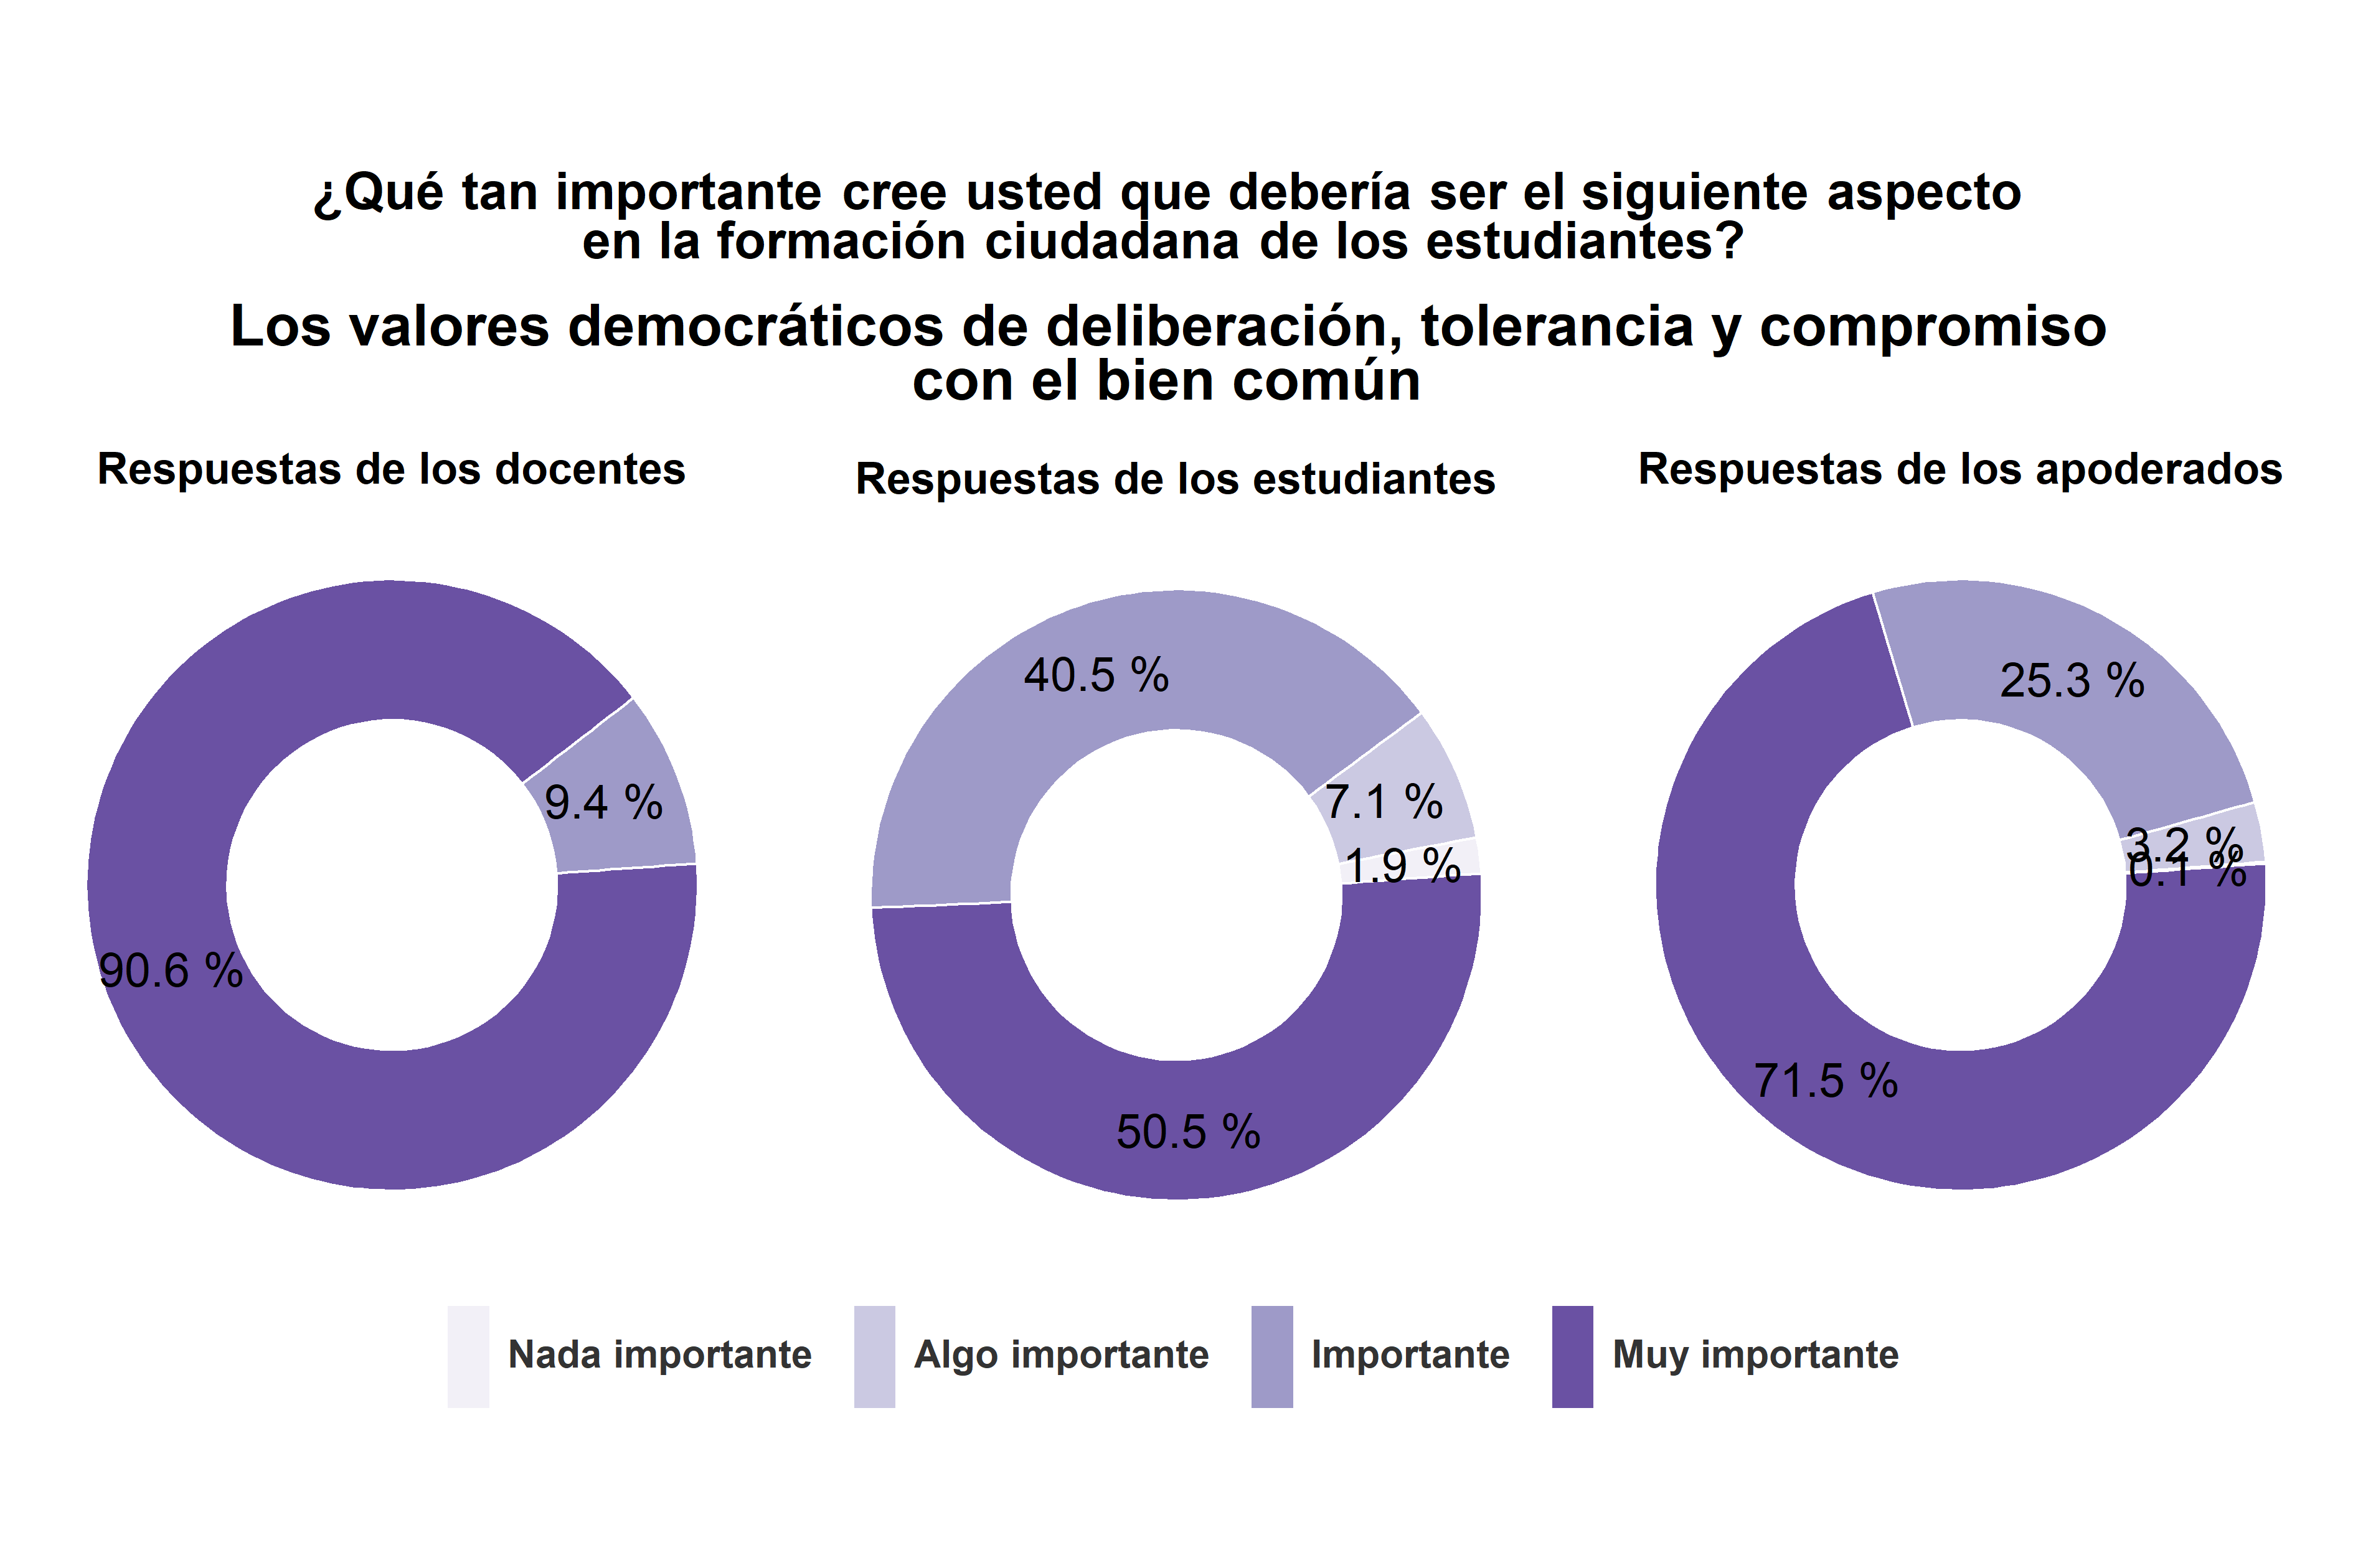
\includegraphics[width=0.8\linewidth,]{images/graph_for_ciud2} 

}

\caption{Relevancia de los valores democráticos}\label{fig:unnamed-chunk-26}
\end{figure}

La mayoría de los docentes y apoderados considera que \emph{los valores democráticos de deliberación, tolerancia y compromiso con el bien común} son un aspecto muy importante en la formación ciudadana de los estudiantes. La opinión de los docentes es más homogénea que la de los estudiantes y la de los apoderados, ya que la totalidad de los profesores declaró que es un aspecto importante o muy importante. En cambio, si bien la mayor parte de los estudiantes y apoderados cree que es un aspecto muy importante (el 50.5\% y el 71.5\%, respectivamente), en ambos grupos algunas personas declararon que es nada importante o algo importante.

\begin{center}\rule{0.5\linewidth}{0.5pt}\end{center}

\begin{figure}[!ht]

{\centering 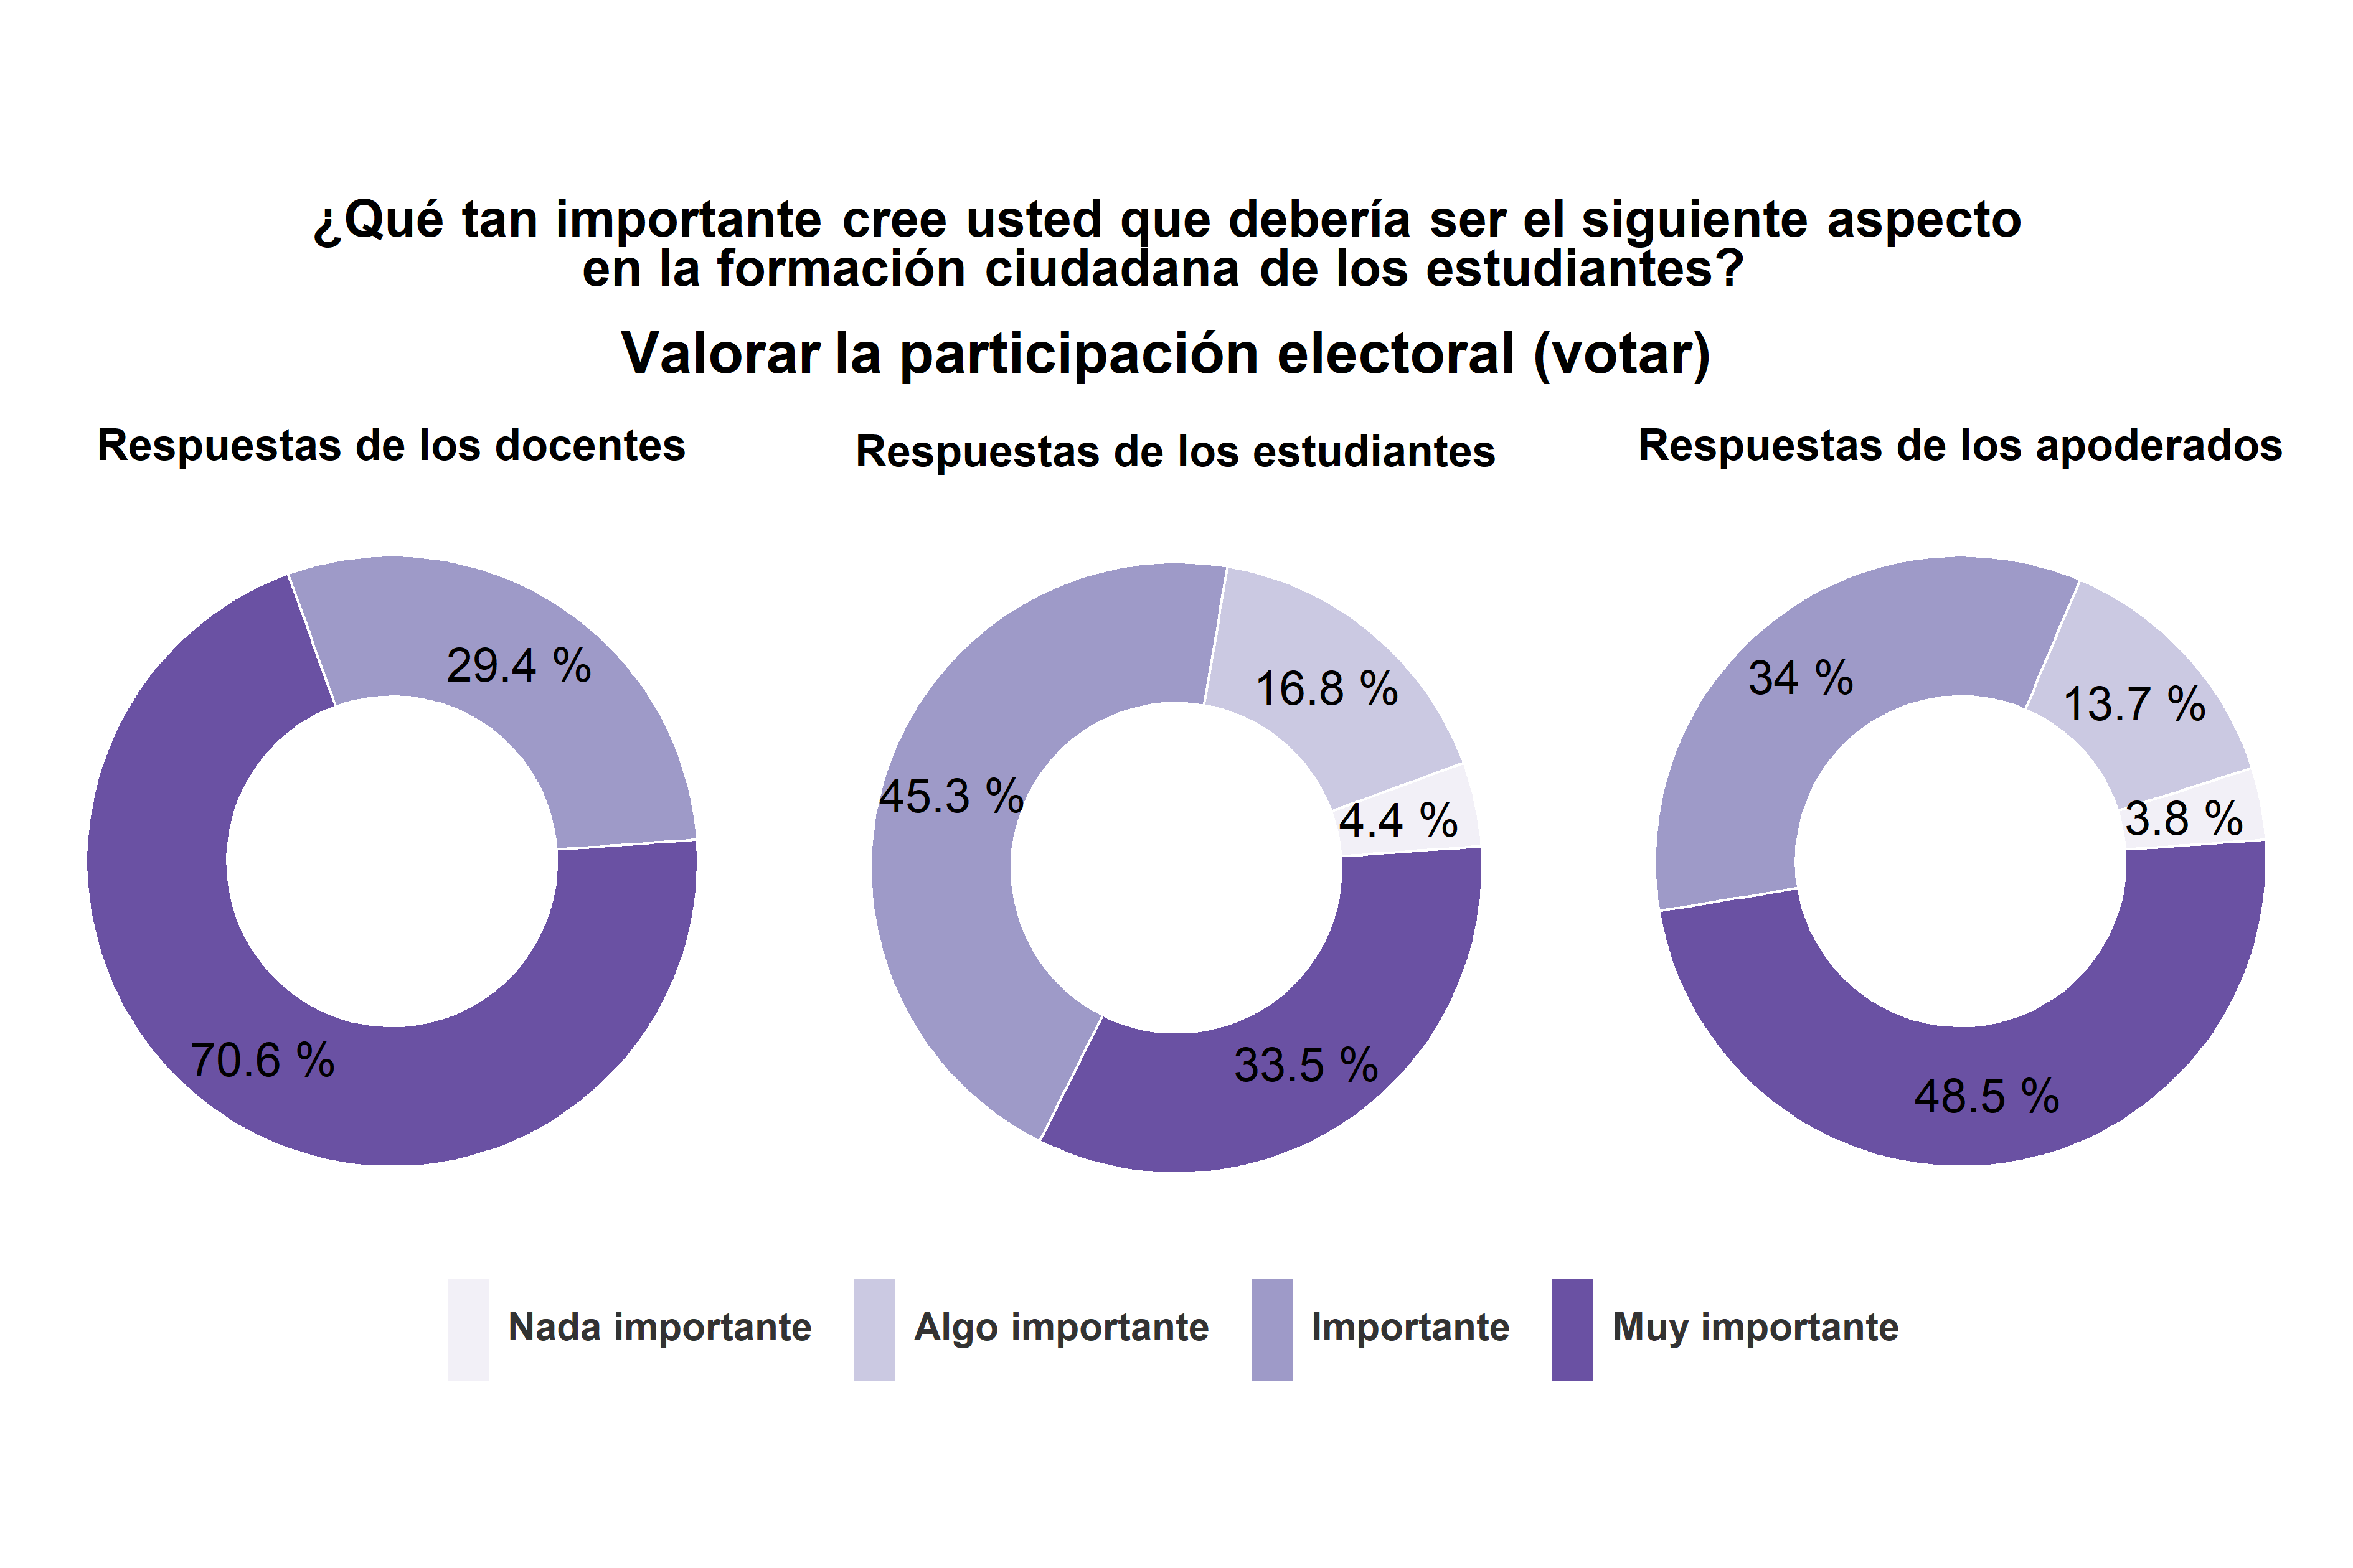
\includegraphics[width=0.8\linewidth,]{images/graph_for_ciud3} 

}

\caption{Relevancia de la participación electoral}\label{fig:unnamed-chunk-27}
\end{figure}

La mayoría de los docentes piensa que \emph{valorar la participación electoral} es un aspecto muy importante en la formación ciudadana de los estudiantes. De hecho, todos los docentes declararon que es un aspecto importante o muy importante. Las opiniones de los estudiantes y apoderados fueron más variadas. Si bien la mayor parte de las respuestas de los estudiantes y de los apoderados se concentraron en las categorías importante (un 43.5\% y un 30.9\%, respectivamente) y muy importante (un 37.8\% y un 52.7\%, respectivamente), un 18.7\% de los estudiantes y un 16.4\% de los apoderados señaló que es un aspecto nada importante o algo importante.

\begin{center}\rule{0.5\linewidth}{0.5pt}\end{center}

\begin{figure}[!ht]

{\centering 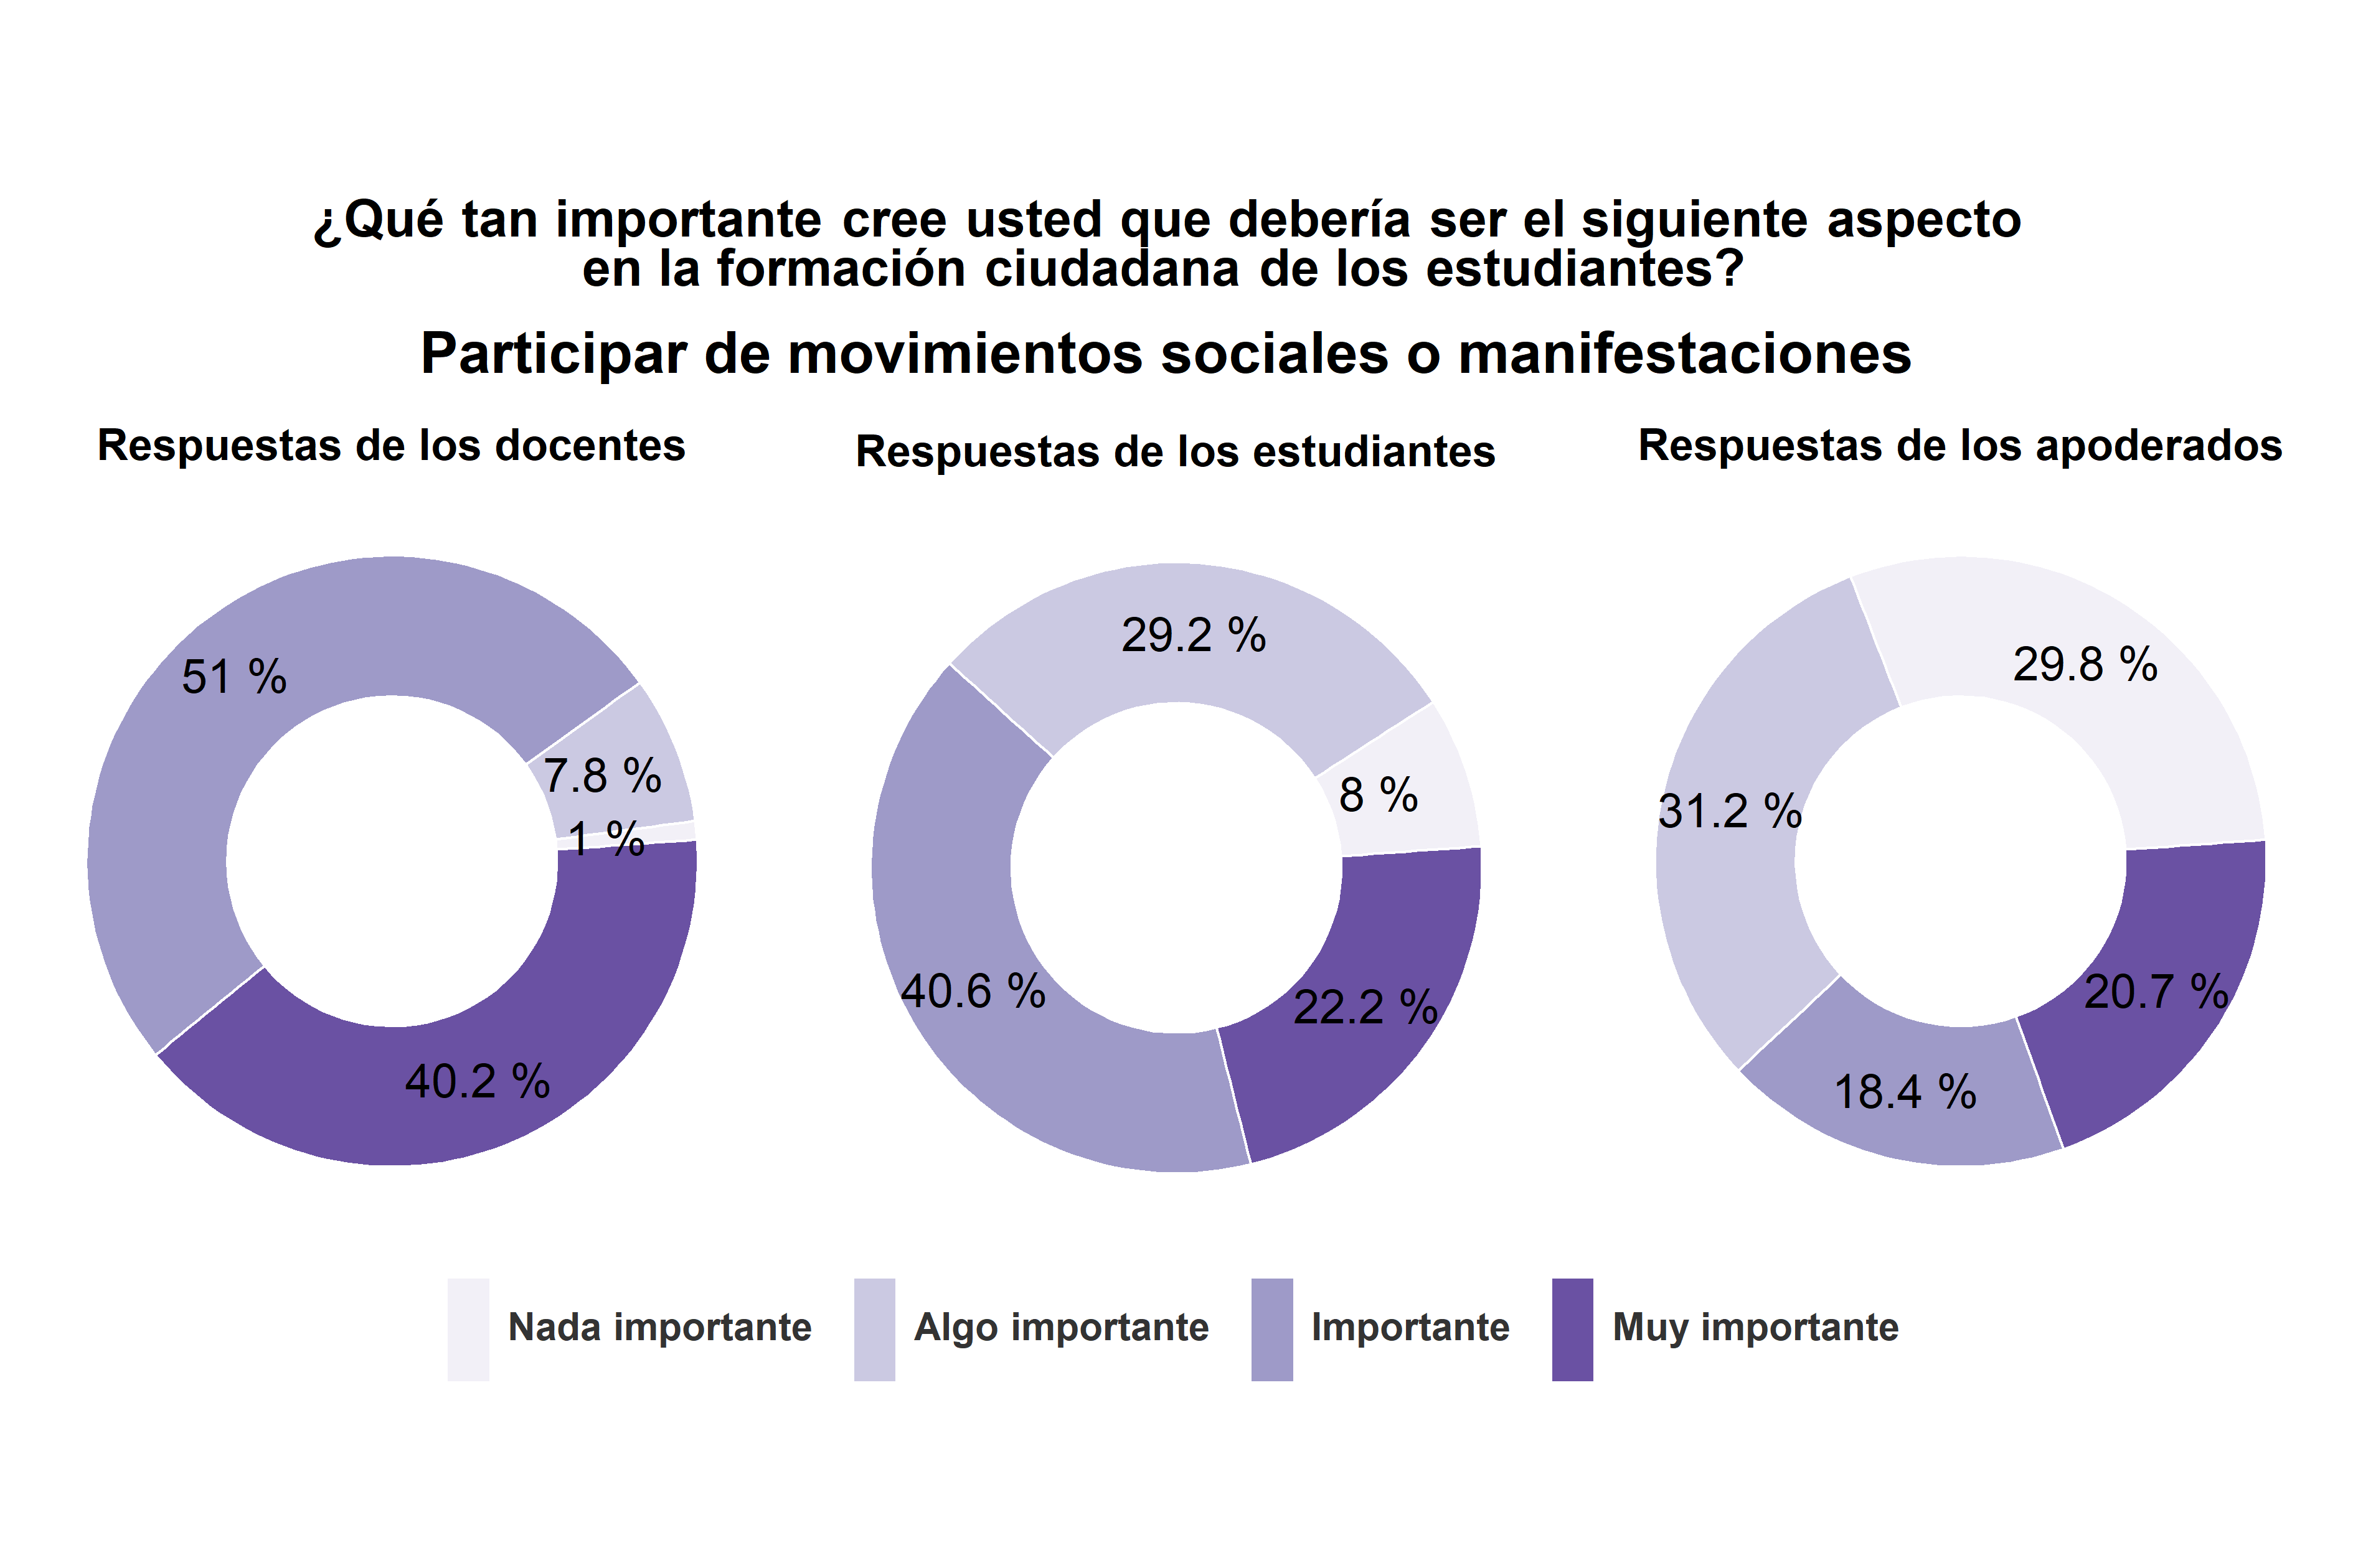
\includegraphics[width=0.8\linewidth,]{images/graph_for_ciud4} 

}

\caption{Relevancia de los movimientos sociales}\label{fig:unnamed-chunk-28}
\end{figure}

La mayoría de los docentes y estudiantes cree que \emph{participar de movimientos sociales} es un aspecto importante o muy importante en la formación ciudadana de los estudiantes, mientras que la mayoría de los apoderados cree que es un aspecto nada importante o algo importante. Los docentes son quienes más valoran la importancia de este aspecto en la formación ciudadana, el 48.7\% declaro que es importante y el 41\% que es muy importante. La mayor parte de los estudiantes piensa que es un aspecto importante (un 40.1\%) o muy importante (un 25.1\%), pero hay un gran grupo de estudiantes que cree que es un aspecto algo importante (27.9\%) o nada importante (un 6.9\%). Por el contrario, la mayor parte de los apoderados cree que es un aspecto algo importante (un 29\%) o nada importante (un 28.6\%), pero hay un gran grupo de apoderados que piensa que es importante (un 19.2\%) o muy importante (un 23.2\%).

\begin{center}\rule{0.5\linewidth}{0.5pt}\end{center}

\begin{figure}[!ht]

{\centering 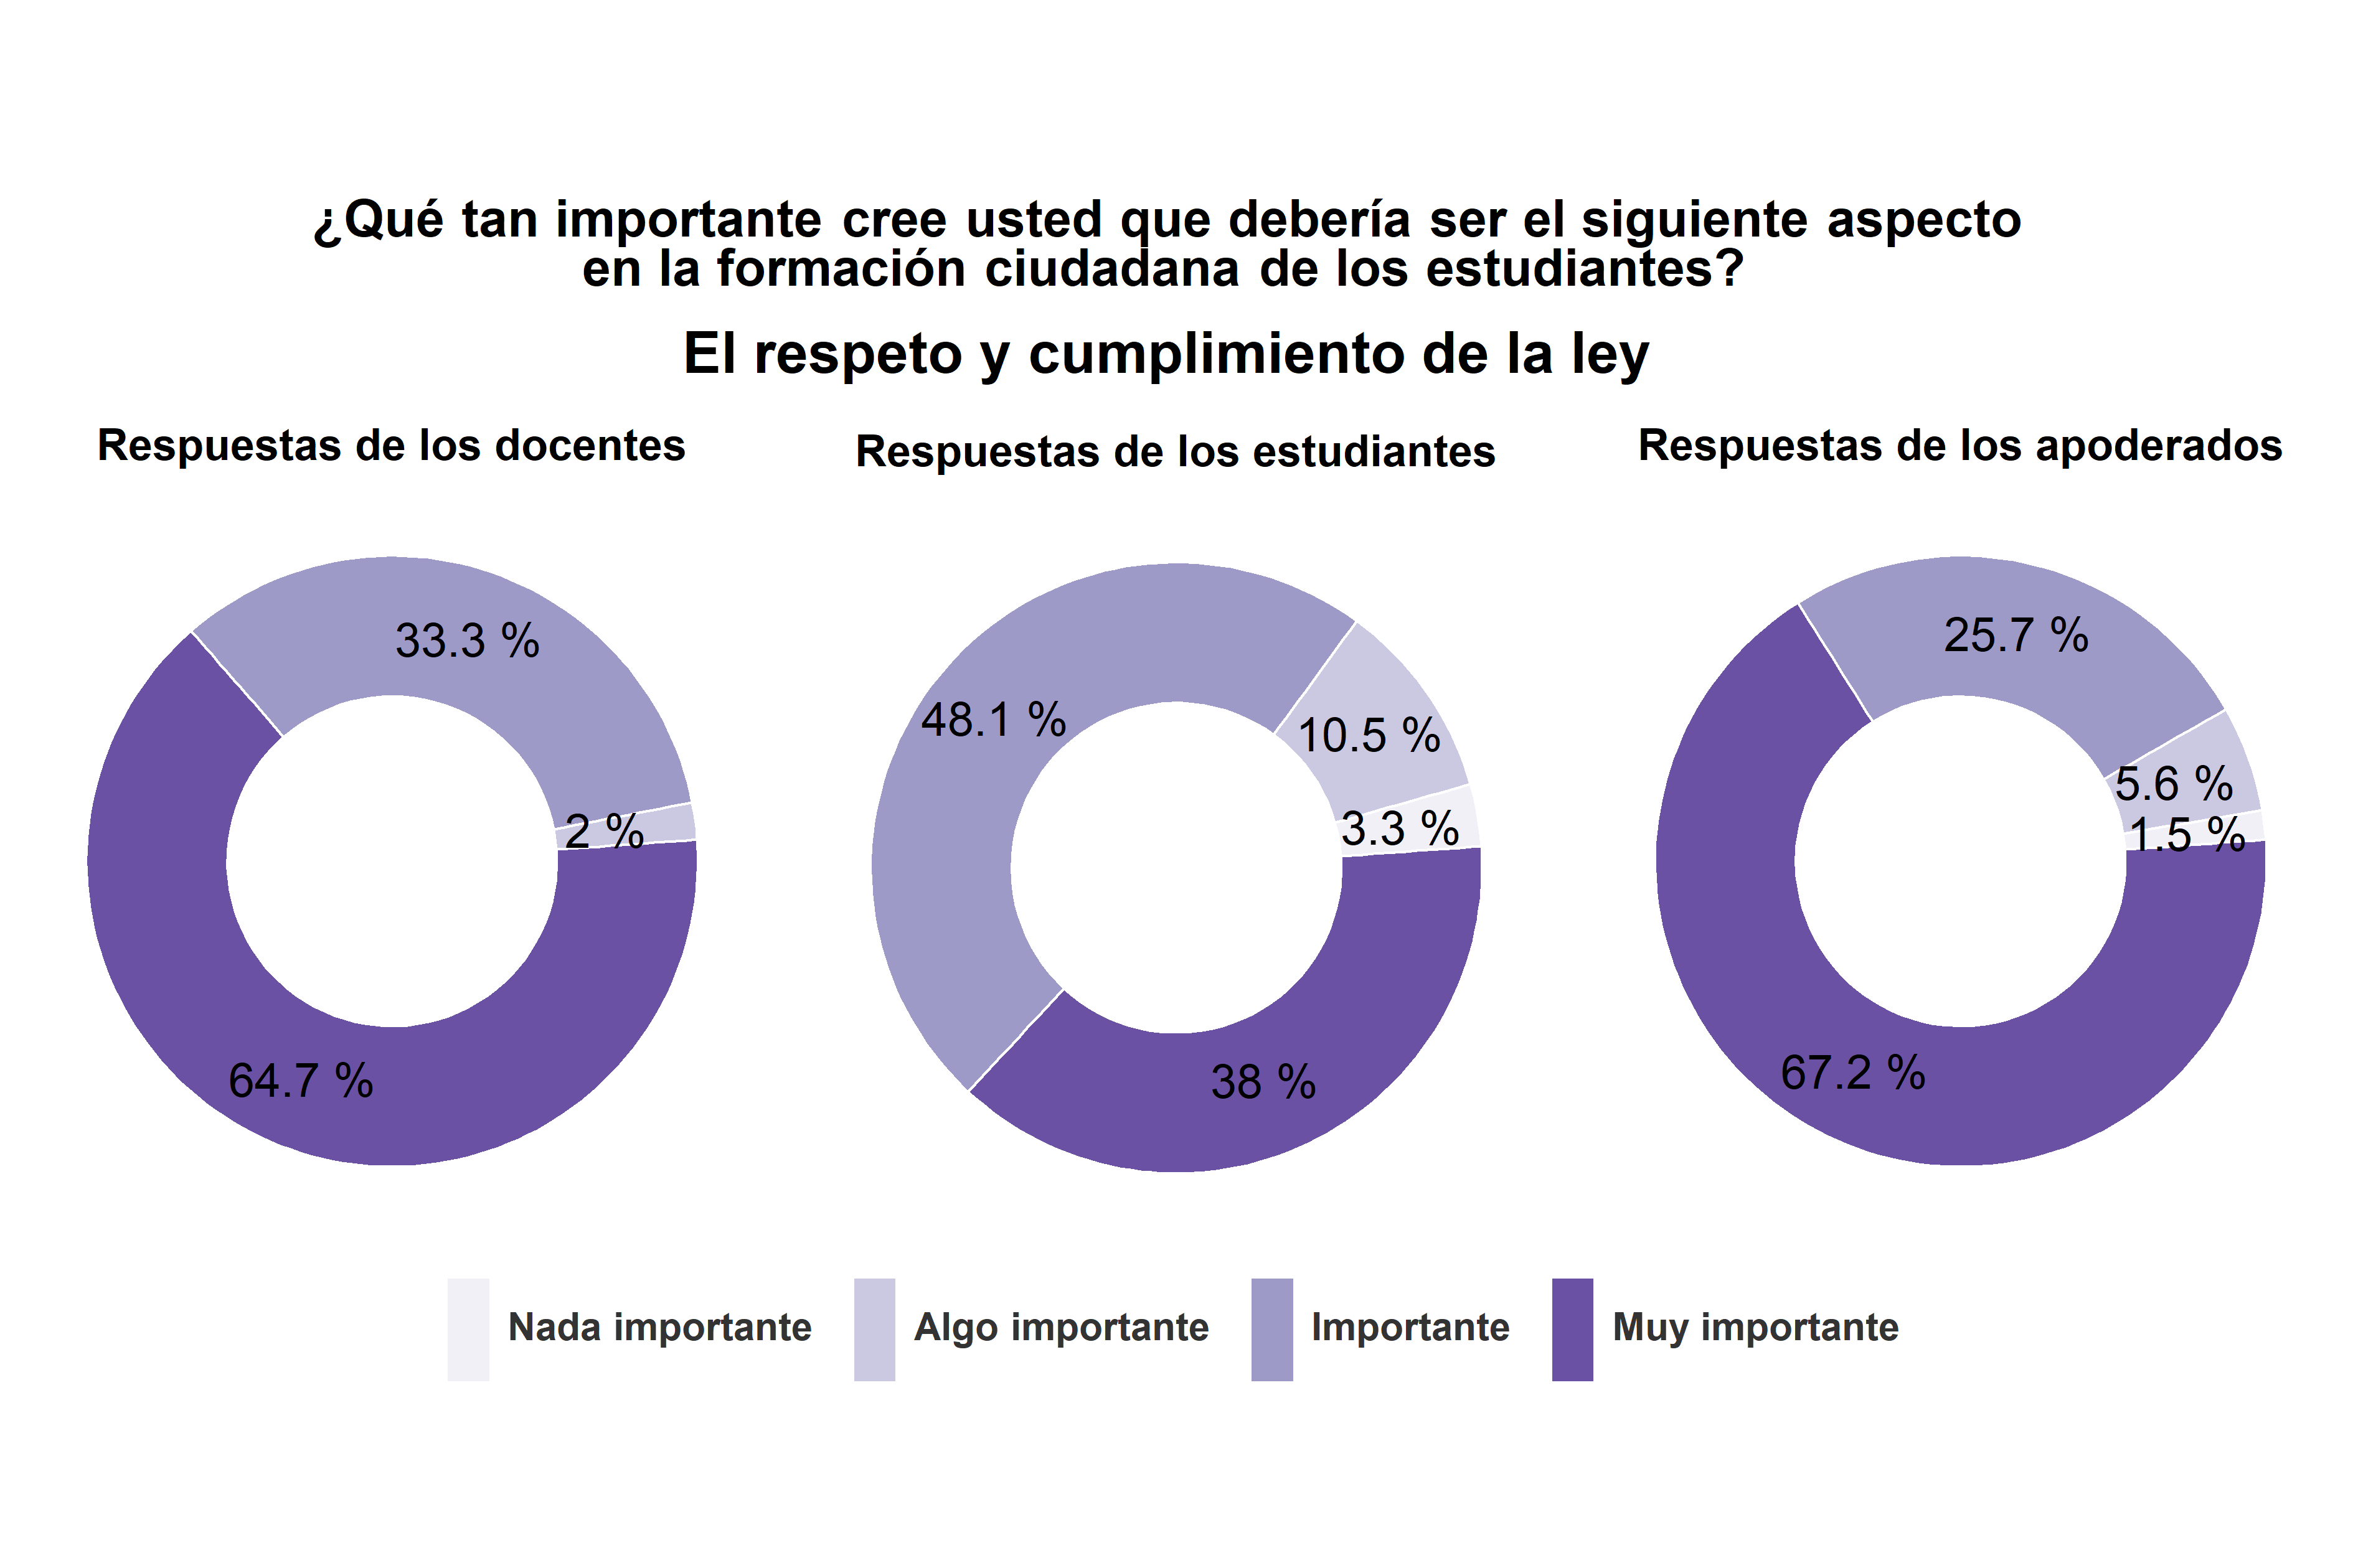
\includegraphics[width=0.8\linewidth,]{images/graph_for_ciud5} 

}

\caption{Relevancia del cumplimiento de la ley}\label{fig:unnamed-chunk-29}
\end{figure}

La mayoría de los docentes y apoderados piensa que \emph{el respeto y cumplimiento de la ley} es un aspecto muy importante en la formación ciudadana de los estudiantes (un 59.3\% y un 68\%, respectivamente). La mayor parte de los estudiantes declaro que es un aspecto importante (un 47.1\%) o muy importante (un 39.6\%).

\begin{center}\rule{0.5\linewidth}{0.5pt}\end{center}

\begin{figure}[!ht]

{\centering 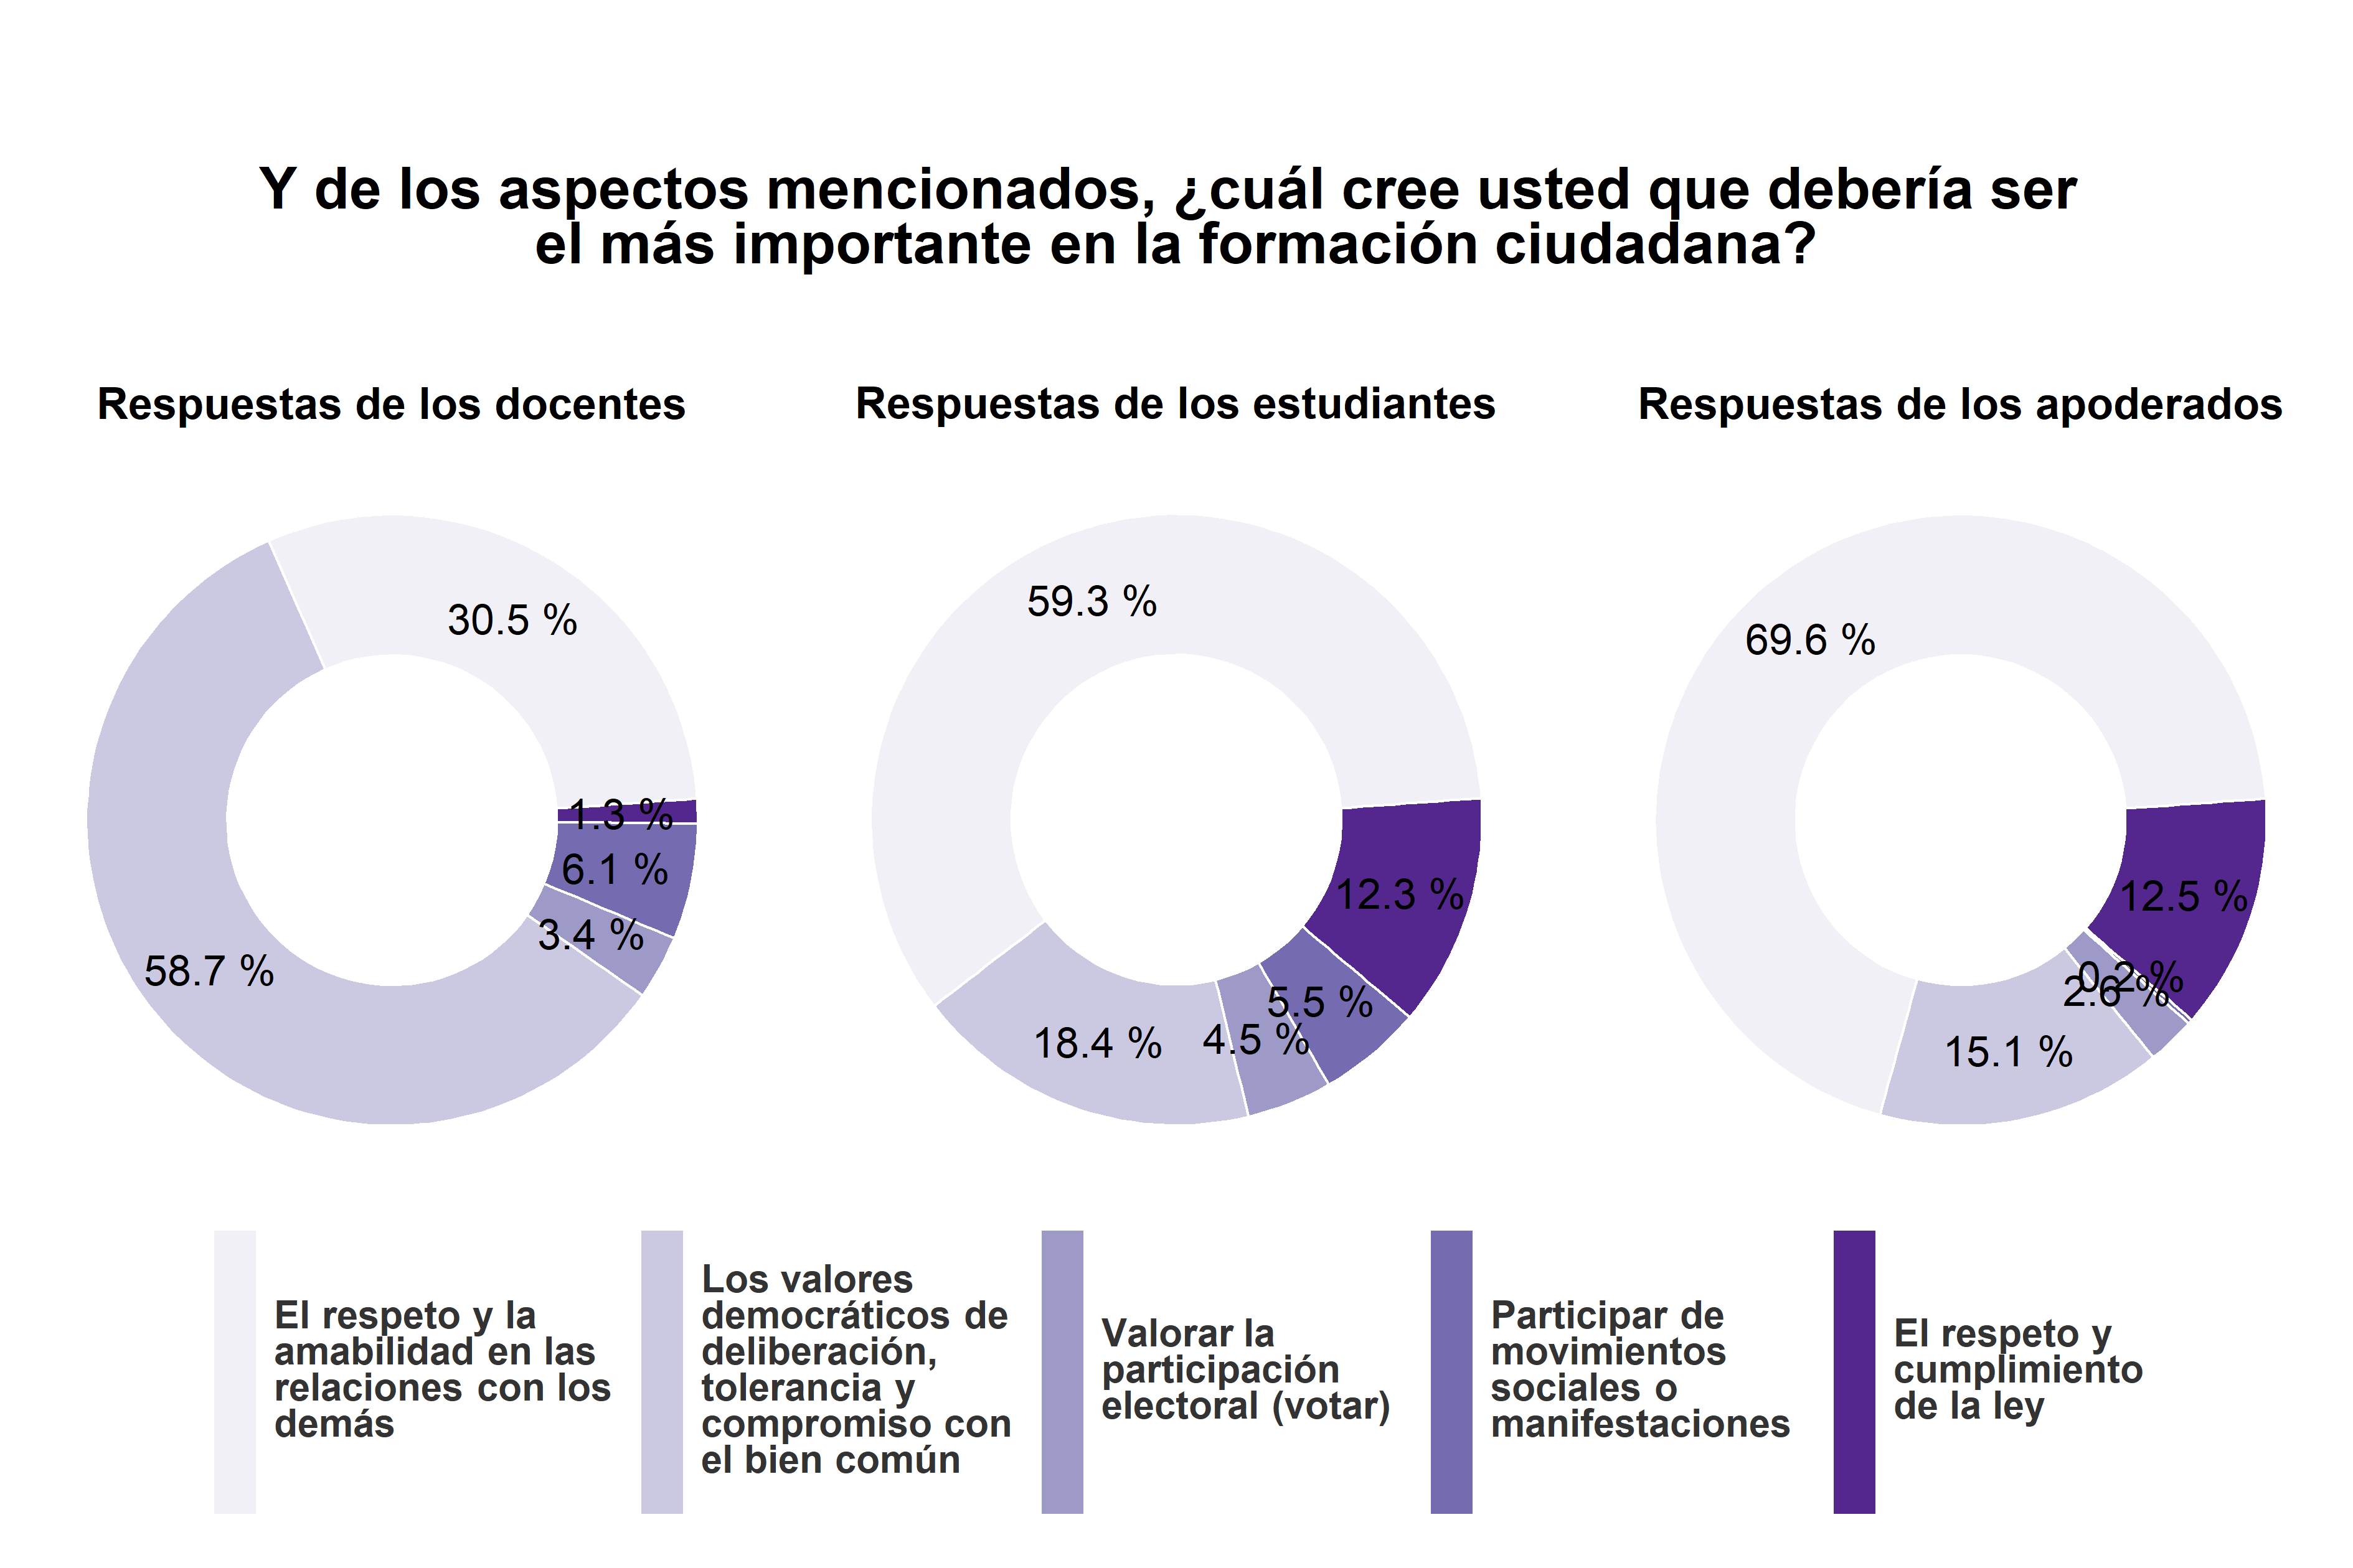
\includegraphics[width=0.8\linewidth,]{images/graph_for_ciud6} 

}

\caption{Aspecto más relevante en la formación ciudadana}\label{fig:unnamed-chunk-30}
\end{figure}

Las respuestas de los estudiantes y apoderados son bastante similares. La mayoría de las personas de ambos grupos cree que el aspecto que debería ser más importante en la formación ciudadana es \emph{el respeto y la amabilidad en las relaciones con los demás} (opción seleccionada por el 59.3\% de los estudiantes y el 69.6\% de los apoderados). Este aspecto también fue destacado por un gran grupo de docentes (un 30.5\%), pero la mayoría de los docentes declaro que el aspecto que debería ser el más importante en la formación ciudadana corresponde a \emph{los valores democráticos de deliberación, tolerancia y compromiso con el bien común} (el 58.7\%).

\begin{center}\rule{0.5\linewidth}{0.5pt}\end{center}

\hypertarget{quiuxe9n-juega-el-rol-muxe1s-importante-en-distintos-aspectos-de-la-formaciuxf3n-ciudadana}{%
\subsection{Quién juega el rol más importante en distintos aspectos de la formación ciudadana}\label{quiuxe9n-juega-el-rol-muxe1s-importante-en-distintos-aspectos-de-la-formaciuxf3n-ciudadana}}

\begin{center}\rule{0.5\linewidth}{0.5pt}\end{center}

\begin{figure}[!ht]

{\centering 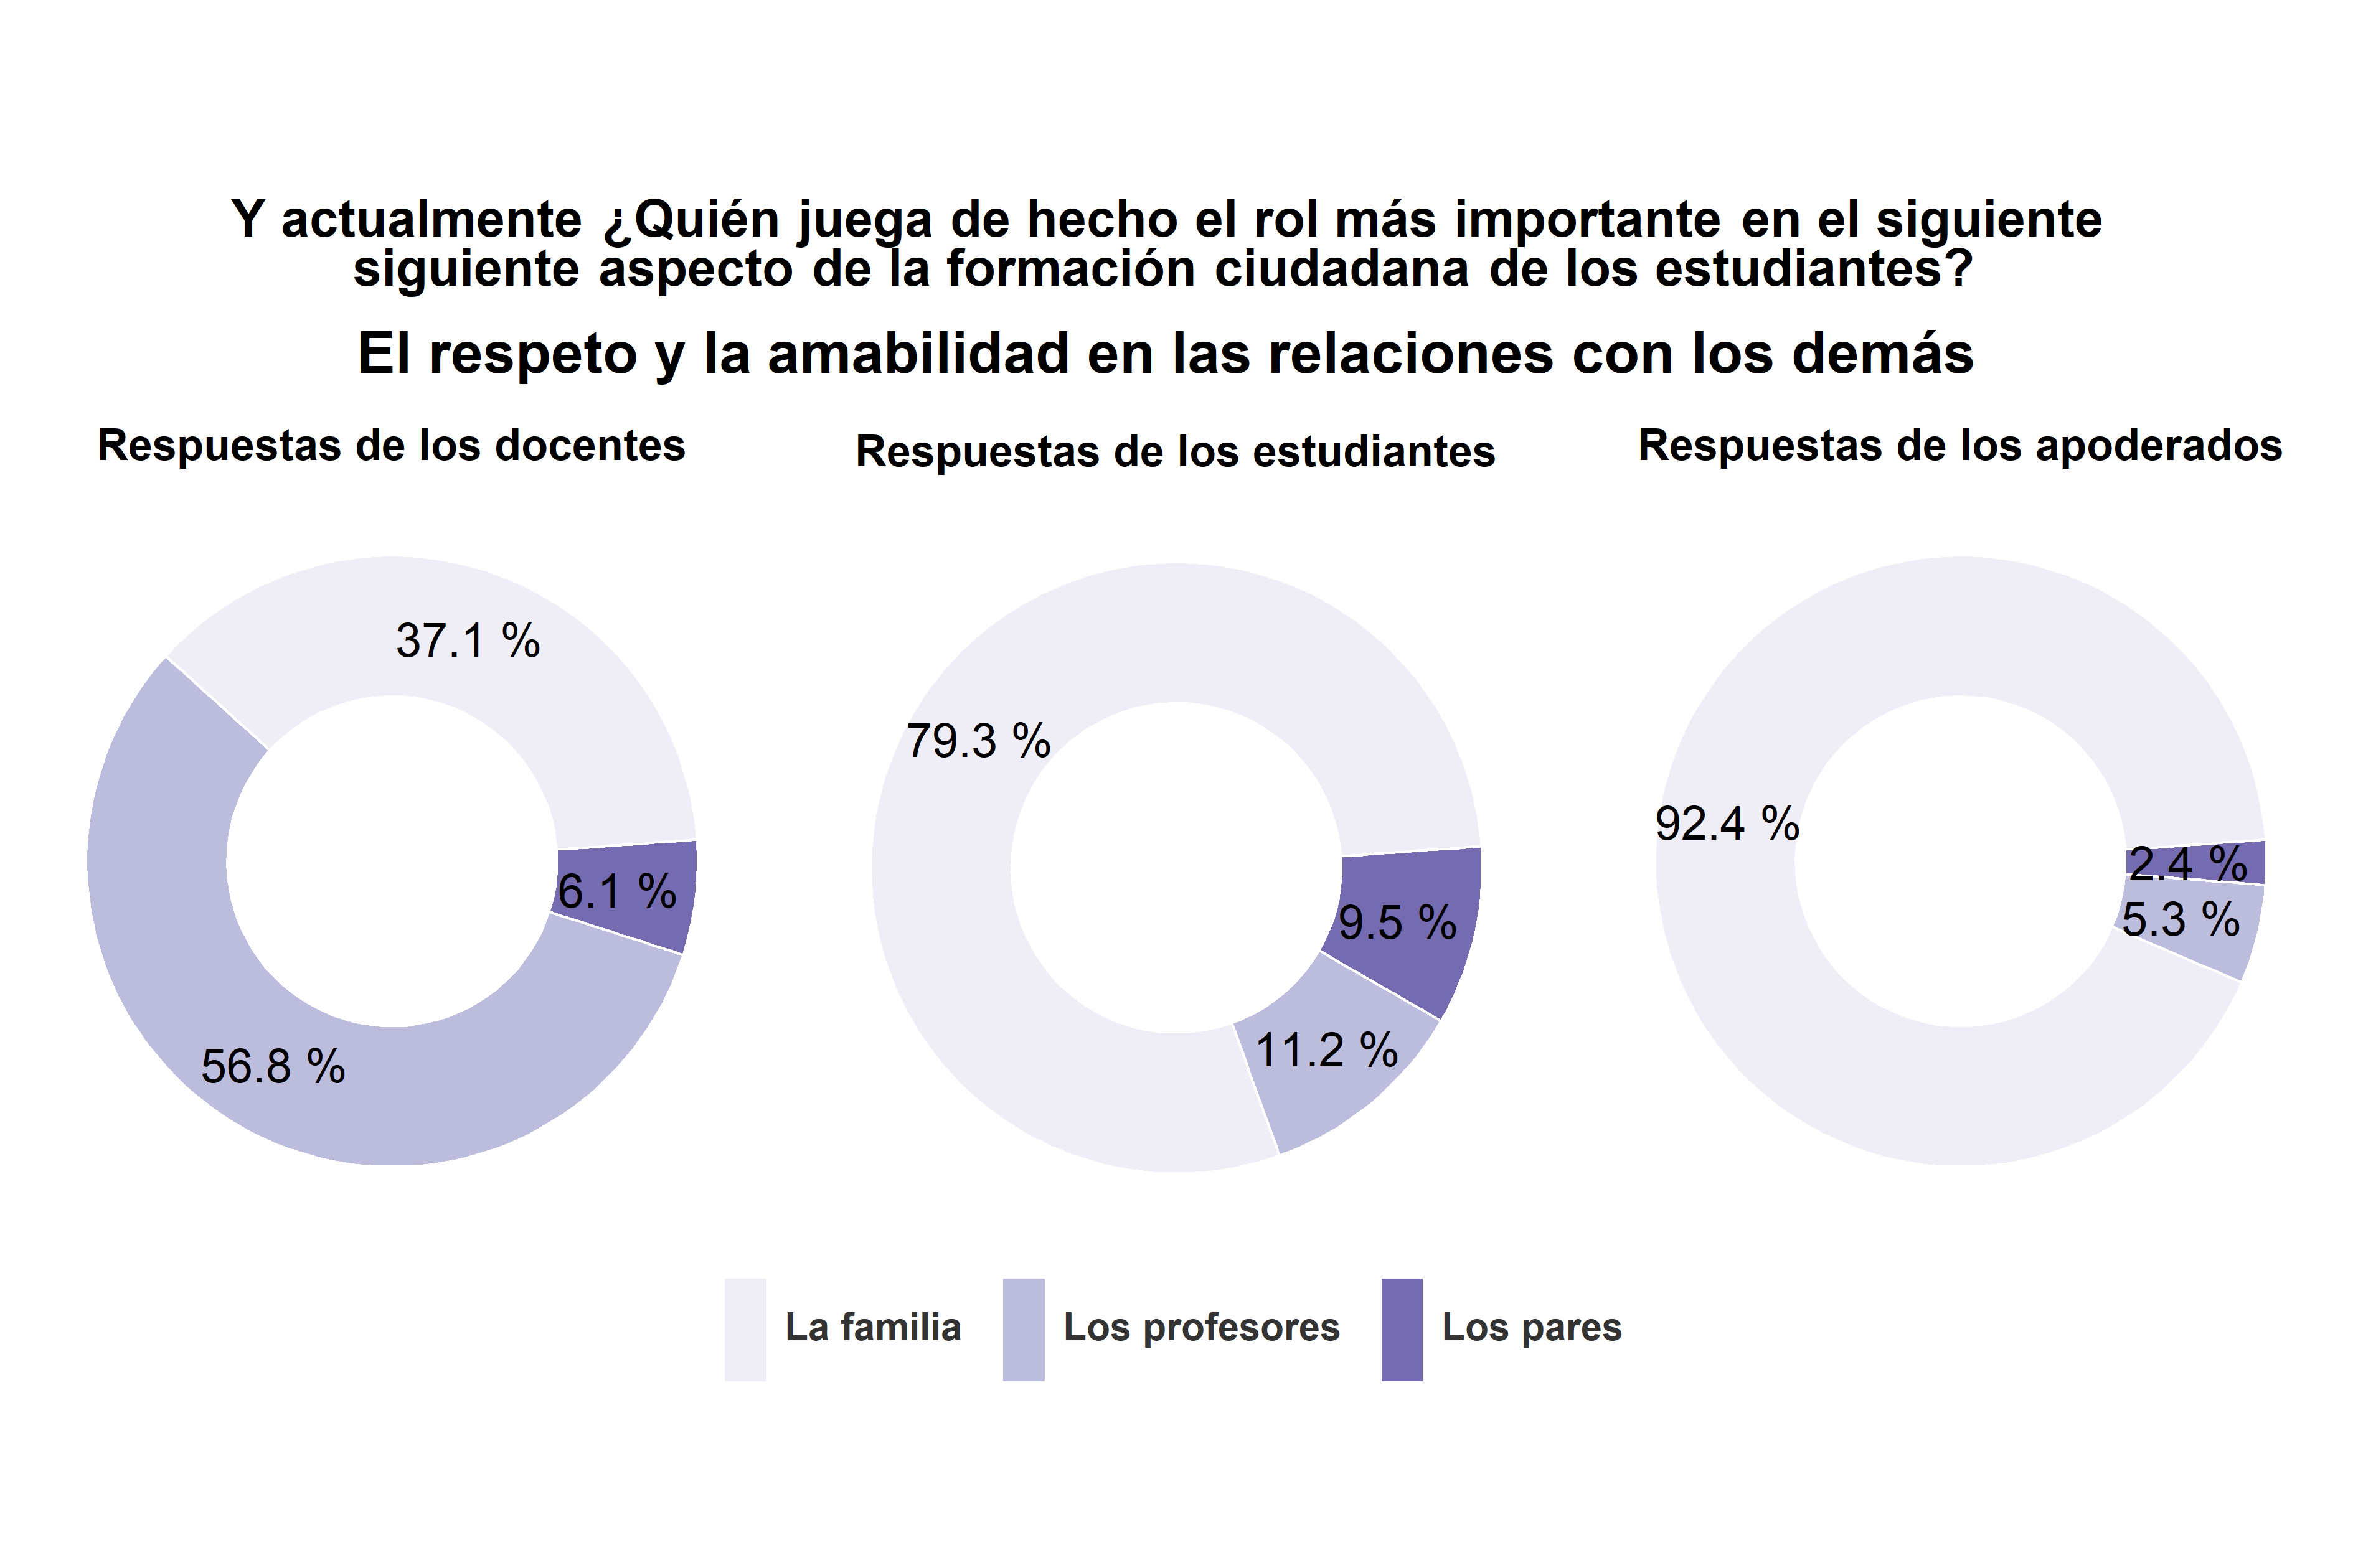
\includegraphics[width=0.8\linewidth,]{images/graph_for_ciud7} 

}

\caption{Quién juega el rol más importante en el respeto en las relaciones con los demás}\label{fig:unnamed-chunk-31}
\end{figure}

La mayoría de los estudiantes y de los apoderados opina que la familia es quien juega de hecho el rol más importante en la enseñanza del \emph{respeto y la amabilidad en las relaciones con los demás} (el 79.3\% y el 92.4\%, respectivamente). Mientras que la mayoría de los docentes piensa que son los profesores quienes juegan de hecho el rol más importante en la enseñanza de este aspecto de la formación ciudadana (el 56.8\%). No obstante, hay una gran proporción de docentes que opina que es la familia quien juega el rol más importante en este aspecto (el 37.1\%).

\begin{center}\rule{0.5\linewidth}{0.5pt}\end{center}

\begin{figure}[!ht]

{\centering 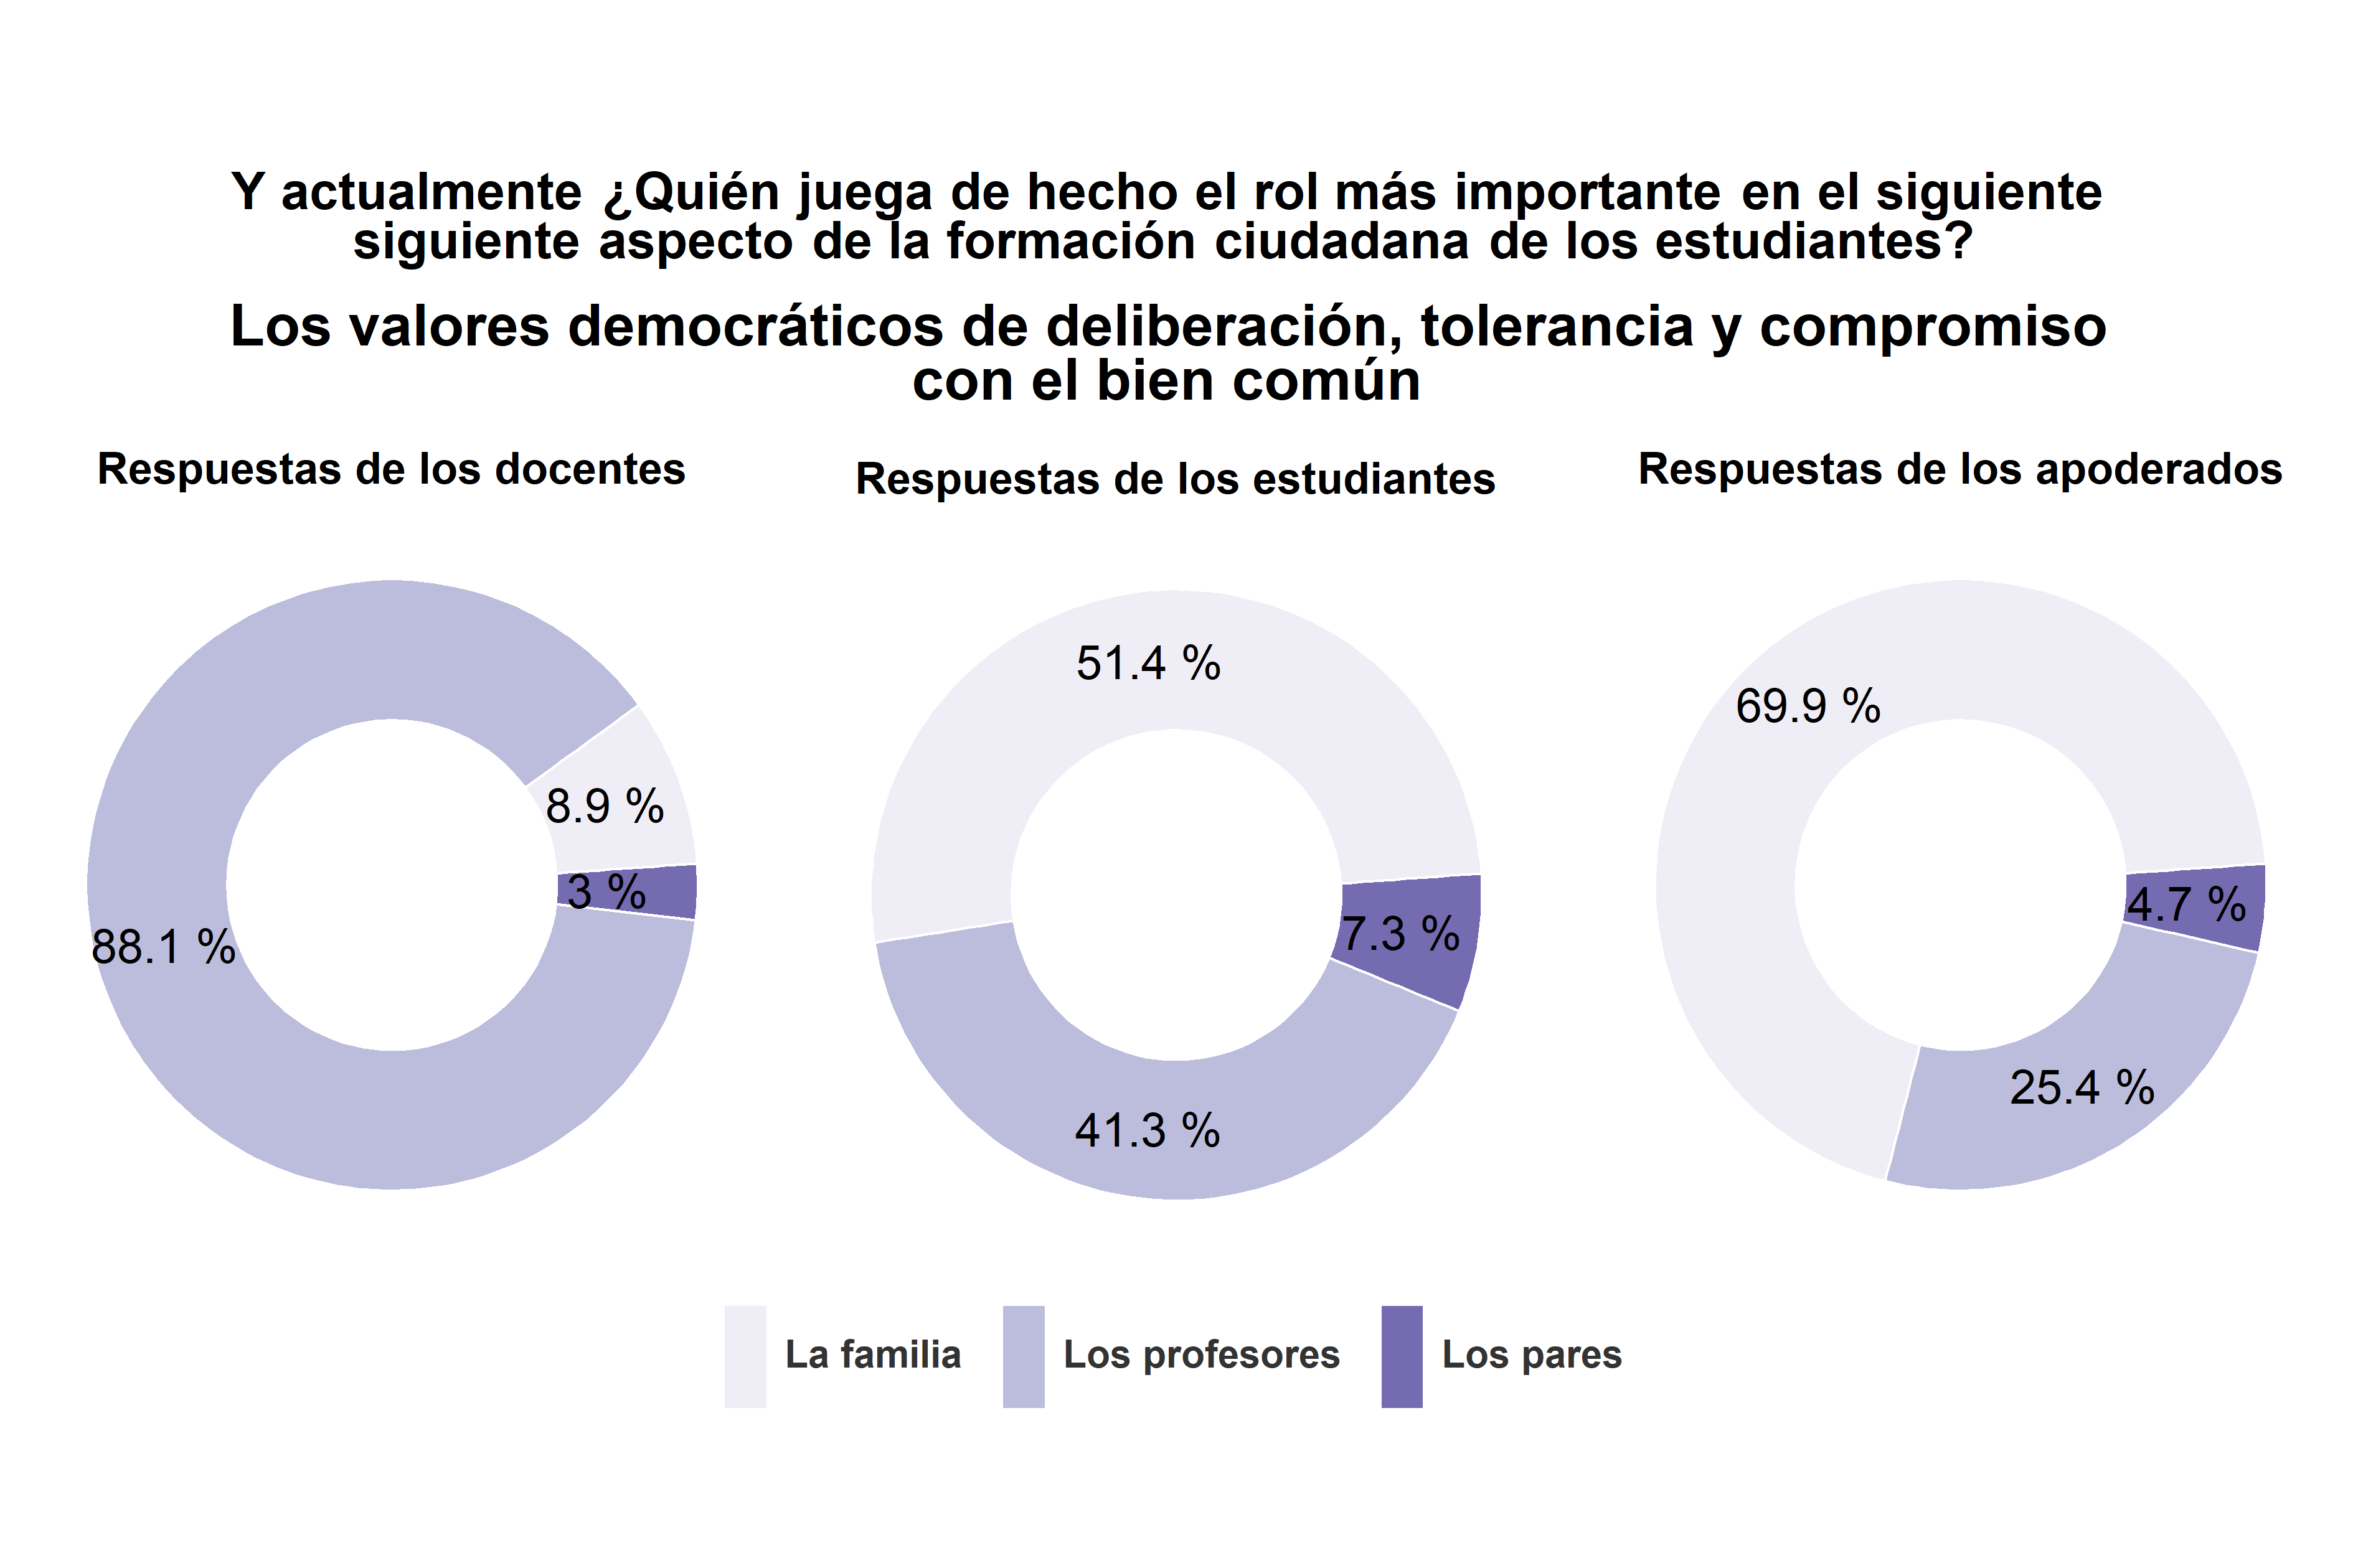
\includegraphics[width=0.8\linewidth,]{images/graph_for_ciud8} 

}

\caption{Quién juega el rol más importante en los valores democráticos}\label{fig:unnamed-chunk-32}
\end{figure}

La mayoría de los estudiantes y de los apoderados cree que es la familia quien juega de hecho el rol más importante en la enseñanza de \emph{los valores democráticos de deliberación, tolerancia y compromiso con el bien común} (el 52.6\% y el 70\%, respectivamente). Mientras que la mayoría de los docentes piensa que son los profesores quienes juegan de hecho el rol más importante en la enseñanza de este aspecto de la formación ciudadana (el 92.6\%). Igualmente, cabe destacar que una gran proporción de estudiantes opina que son los profesores quienes juegan de hecho el rol más importante en este aspecto (el 41.6\%).

\begin{center}\rule{0.5\linewidth}{0.5pt}\end{center}

\begin{figure}[!ht]

{\centering 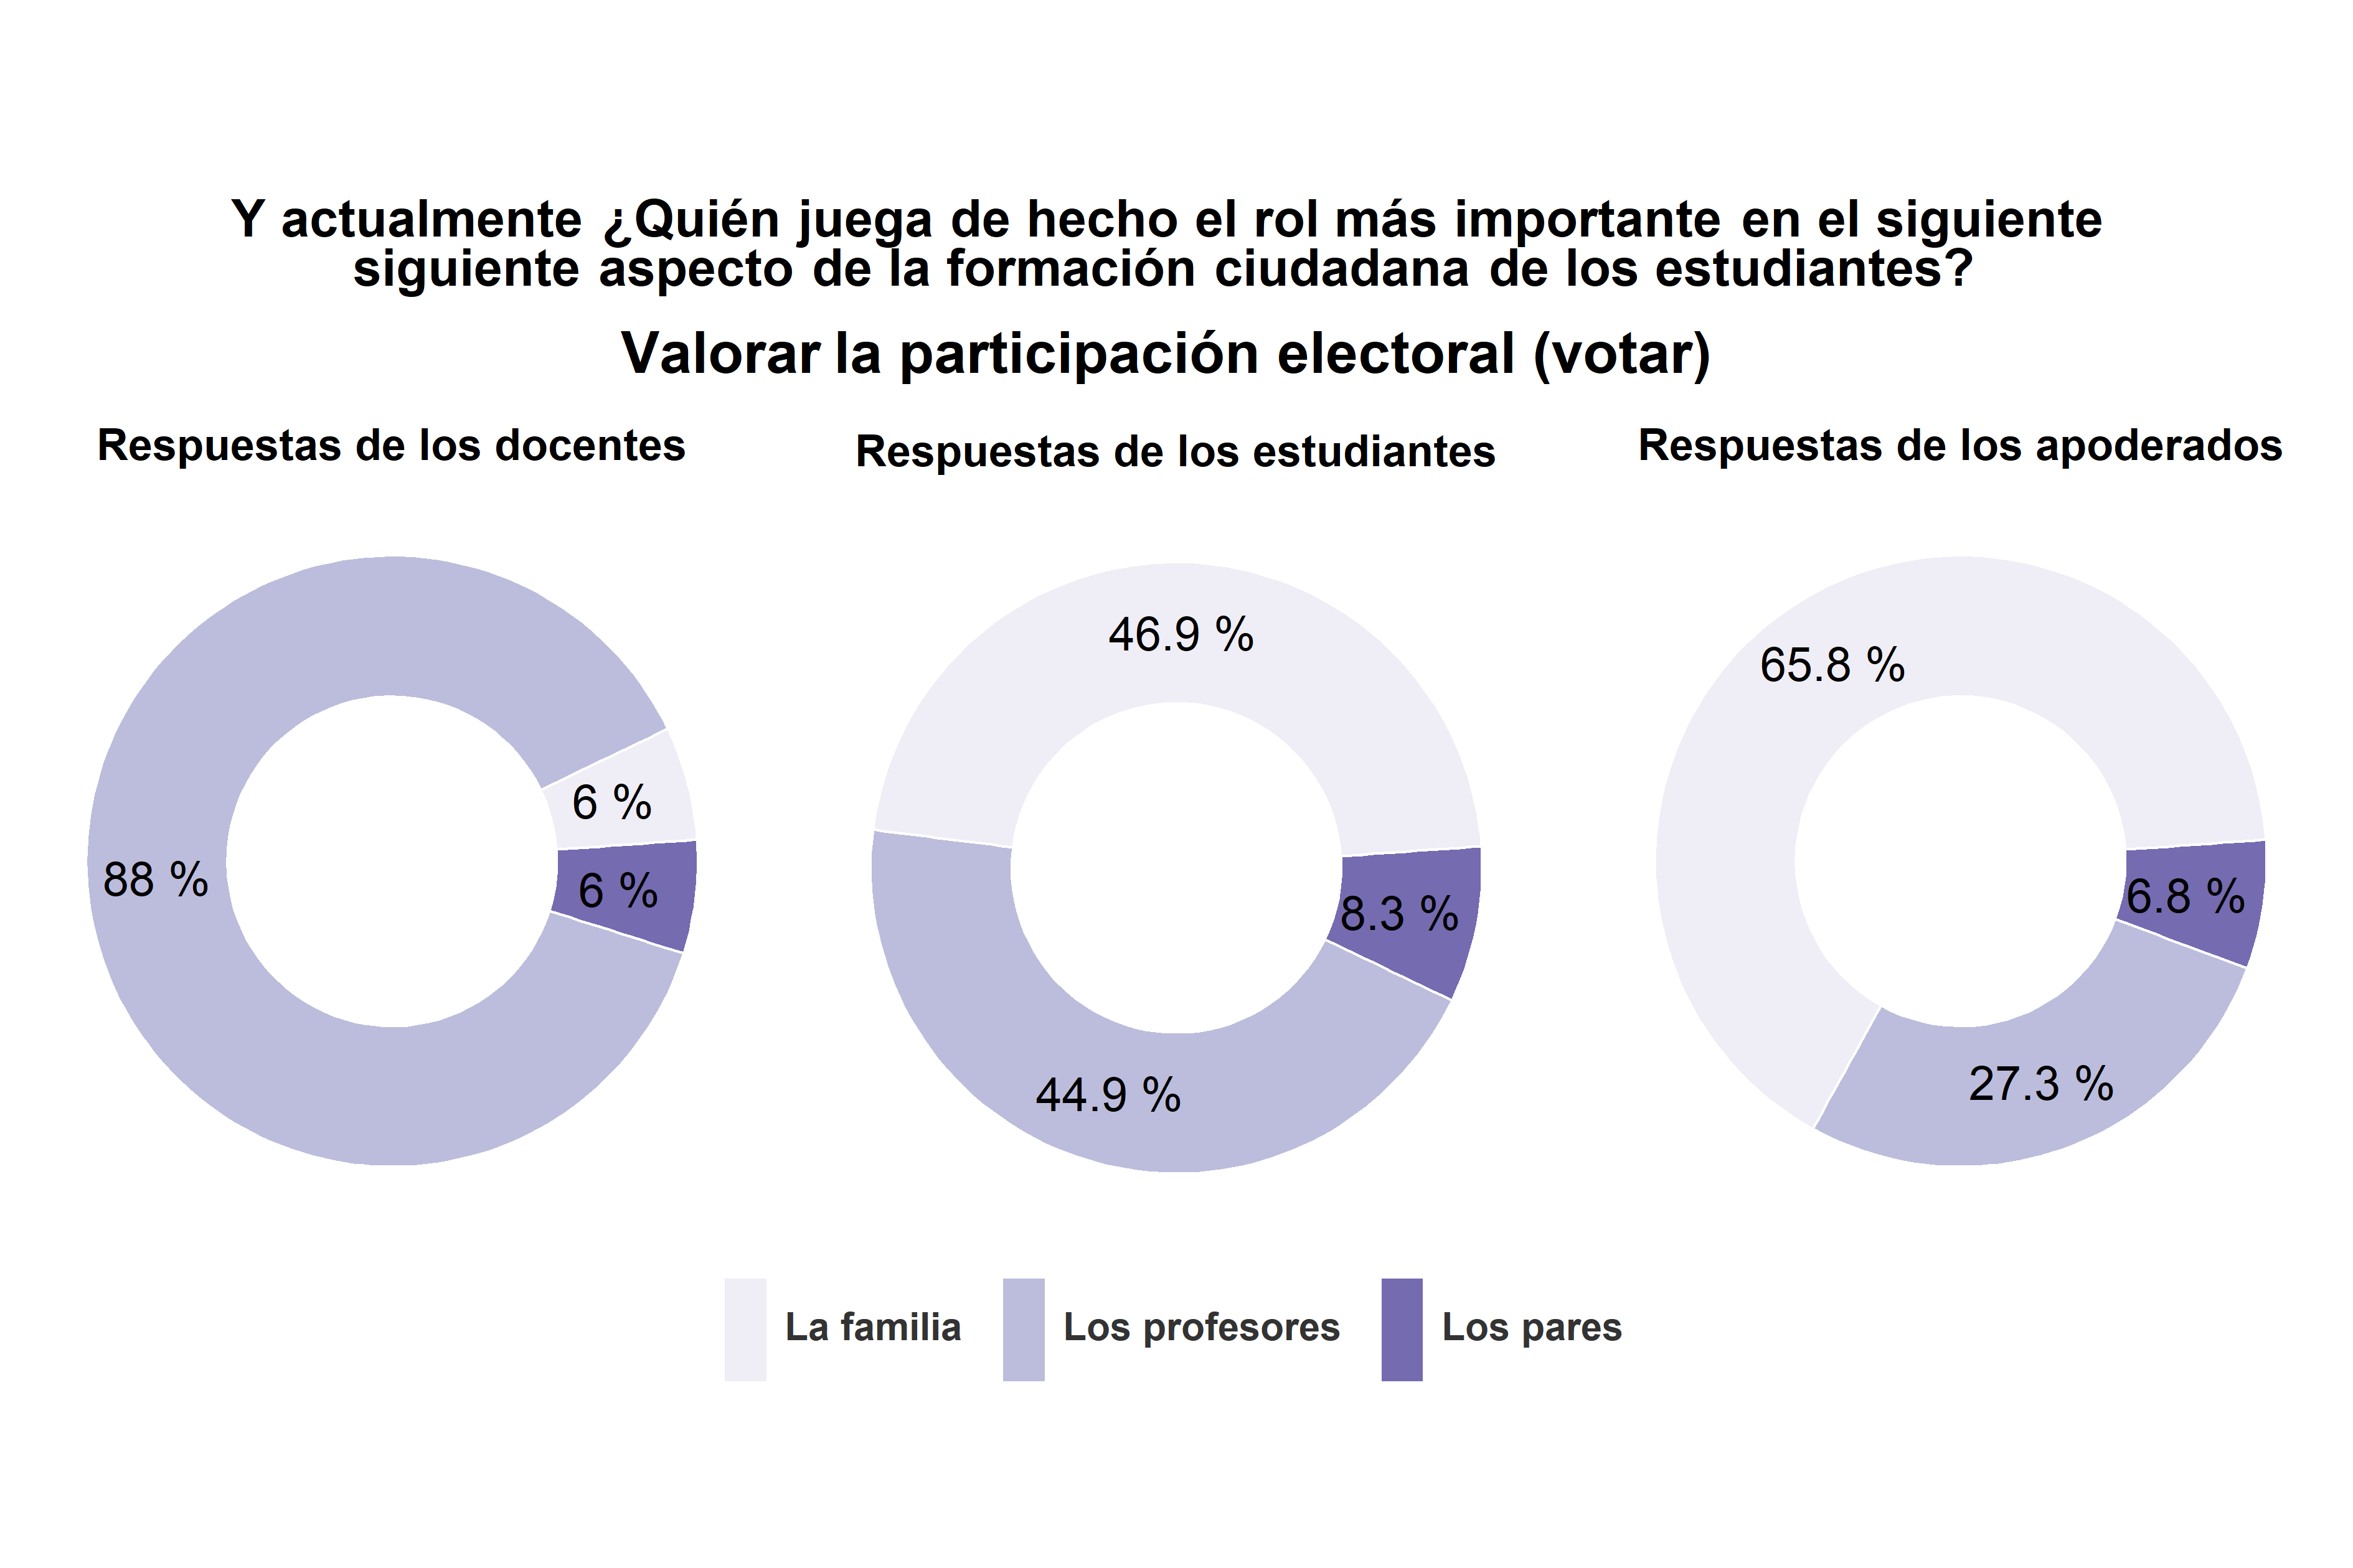
\includegraphics[width=0.8\linewidth,]{images/graph_for_ciud9} 

}

\caption{Quién juega el rol más importante en valorar la participación electoral}\label{fig:unnamed-chunk-33}
\end{figure}

La mayoría de los docentes opina que son los profesores quienes juegan de hecho el rol más importante en la enseñanza de \emph{valorar la participación electoral} (el 92.9\%). Mientras que la mayoría de los apoderados piensa que es la familia quien juega de hecho el rol más importante en la enseñanza de este aspecto de la formación ciudadana (el 63.4\%). La opinión de los estudiantes es más heterogénea. El 47.6\% de los estudiantes cree que es la familia quien juega el rol más importante en la enseñanza de este aspecto y el 45.5\% de los estudiantes cree que son los profesores.

\begin{center}\rule{0.5\linewidth}{0.5pt}\end{center}

\begin{figure}[!ht]

{\centering 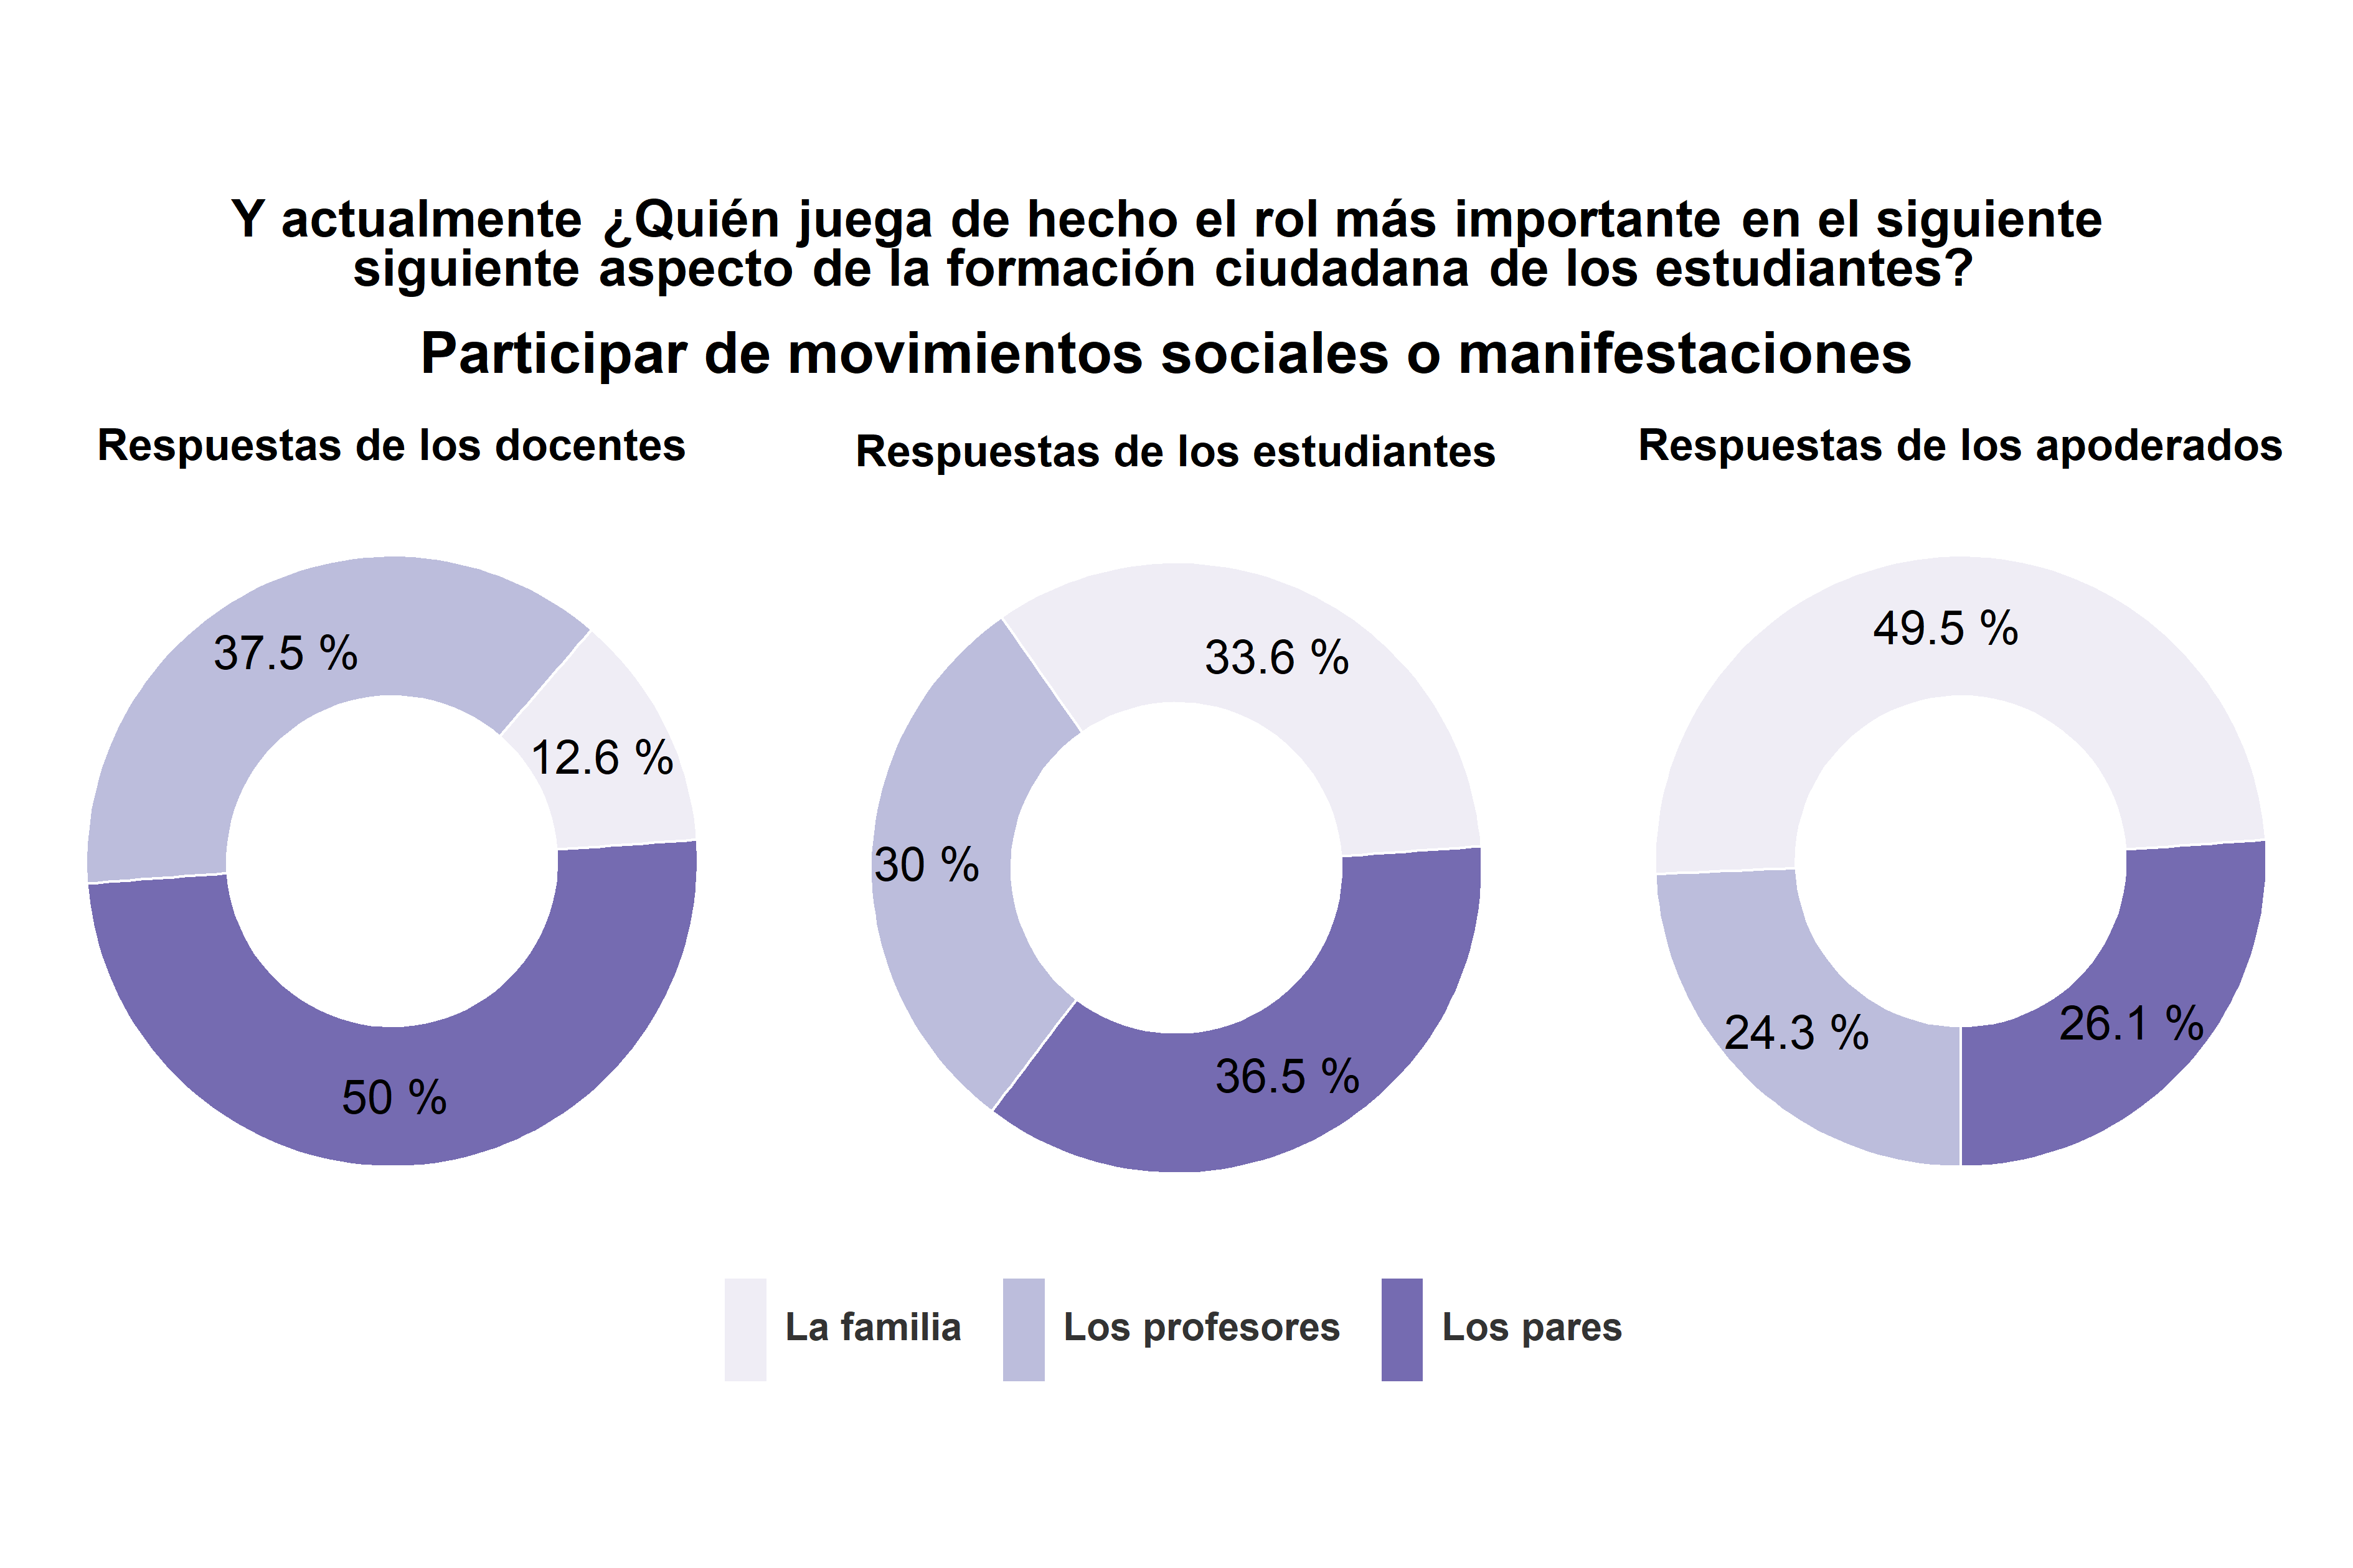
\includegraphics[width=0.8\linewidth,]{images/graph_for_ciud10} 

}

\caption{Quién juega el rol más importante en participar en movimientos sociales}\label{fig:unnamed-chunk-34}
\end{figure}

La mayoría de los docentes (el 50\%) cree que son los pares quienes juegan de hecho el rol más importante en la enseñanza de \emph{participar en movimientos sociales} y un gran grupo de los docentes (el 37.5) cree son los profesores. La opinión de los estudiantes está distribuida de forma equitativa entre las tres alternativas. El 33.6\% de los estudiantes piensa que la familia es quien juega el rol más importante en este aspecto, el 36.5\% piensa que son los pares y el 30\% piensa que son los profesores. La mayor parte de los apoderados (el 49.5\%) opina que es la familia quien juega de hecho el rol más importante en la enseñanza de este aspecto.

\begin{center}\rule{0.5\linewidth}{0.5pt}\end{center}

\begin{figure}[!ht]

{\centering 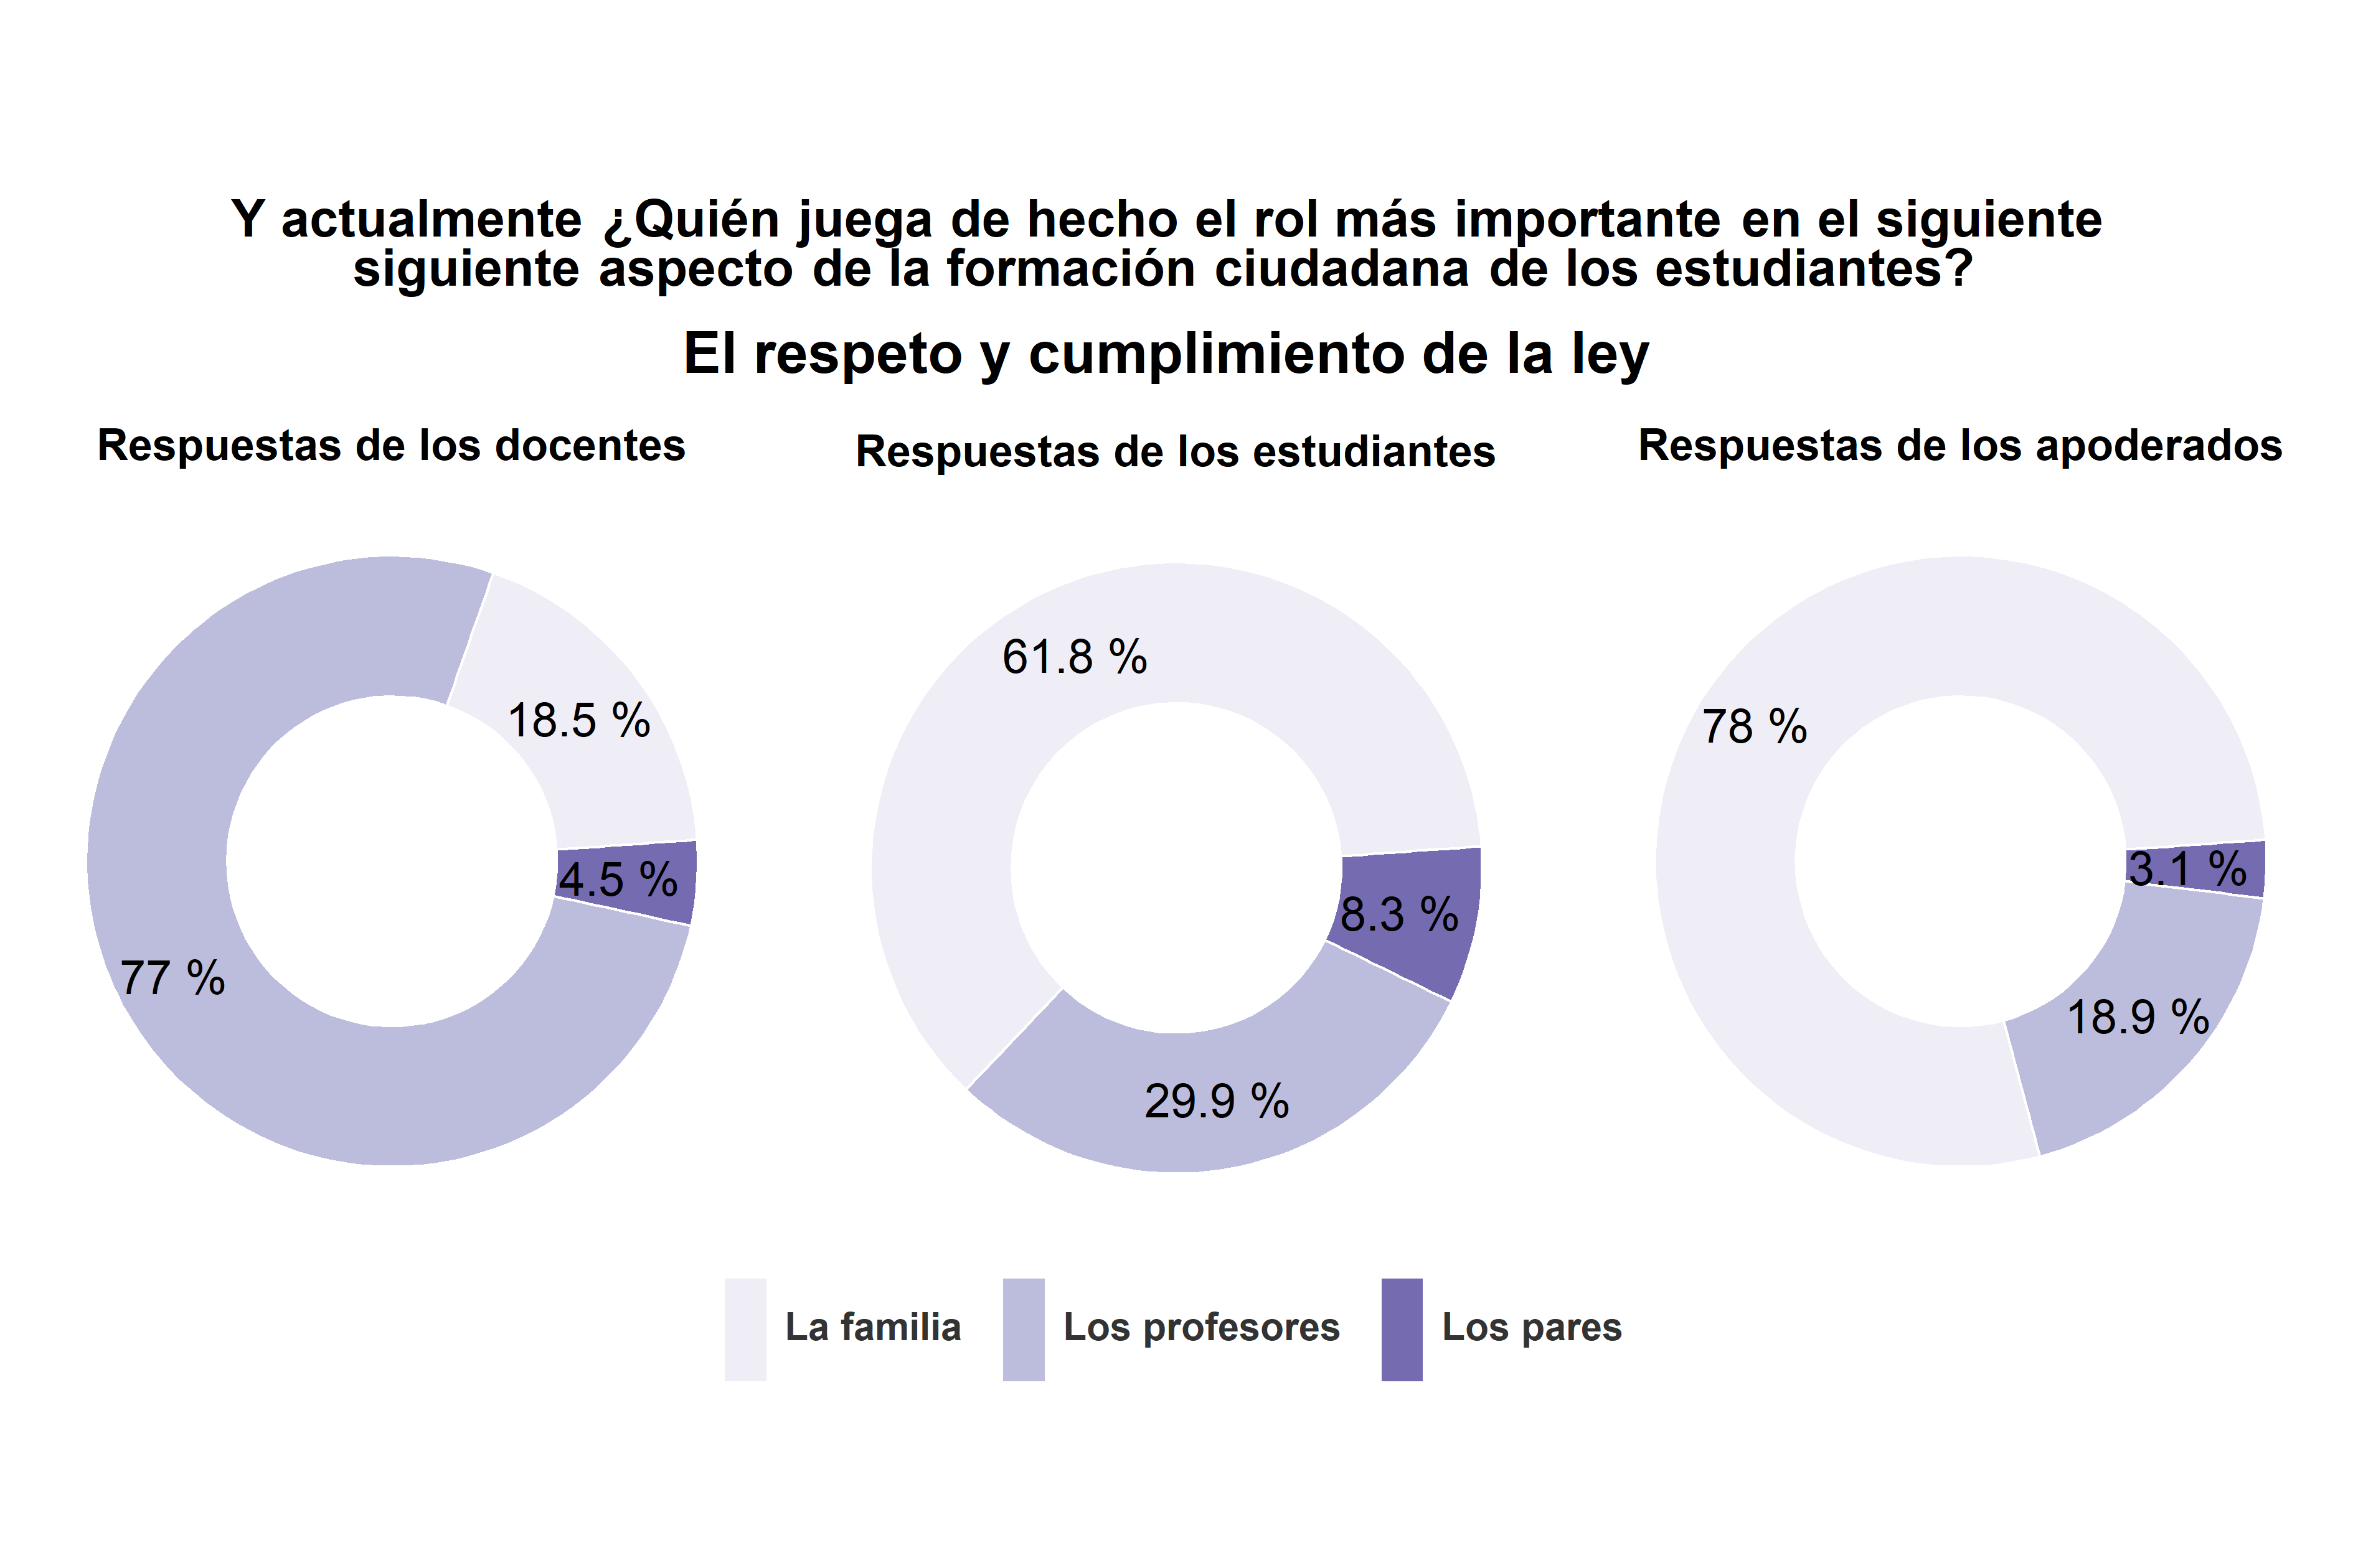
\includegraphics[width=0.8\linewidth,]{images/graph_for_ciud11} 

}

\caption{Quién juega el rol más importante en el cumplimiento de la ley}\label{fig:unnamed-chunk-35}
\end{figure}

La mayoría de los estudiantes y de los apoderados cree que es la familia quien juega de hecho el rol más importante en la enseñanza del \emph{respeto y cumplimiento de la ley} (el 61.8\% y el 78\%, respectivamente). Mientras que la mayoría de los docentes piensa que son los profesores quienes juegan de hecho el rol más importante en la enseñanza de este aspecto de la formación ciudadana (el 77\%).

\begin{center}\rule{0.5\linewidth}{0.5pt}\end{center}

\hypertarget{actitudes-poluxedticas}{%
\chapter{Actitudes políticas}\label{actitudes-poluxedticas}}

En este módulo se presentan las respuestas de los docentes, estudiantes y apoderados a una serie de preguntas sobre temas políticos y sociales. El análisis se realizará comparando las respuestas de los grupos. Cabe precisar que algunas de las preguntas fueron realizadas solo a los estudiantes y apoderados.

El reporte de los resultados correspondientes a este módulo se organiza en tres secciones. En la primera sección se presentarán las respuestas a preguntas relativas al interés en la política y al interés en tres distintos problemas sociales. En la segunda sección se expondrán las respuestas a preguntas respecto a la satisfacción con la democracia y distintas actitudes autoritarias. En la tercera sección se mostrarán los resultados de una pregunta sobre la confianza en distintas instituciones, la cual fue presentada solo a los estudiantes.

\hypertarget{interuxe9s-en-poluxedtica-y-problemas-sociales}{%
\section{Interés en política y problemas sociales}\label{interuxe9s-en-poluxedtica-y-problemas-sociales}}

\begin{center}\rule{0.5\linewidth}{0.5pt}\end{center}

\begin{figure}[!ht]

{\centering 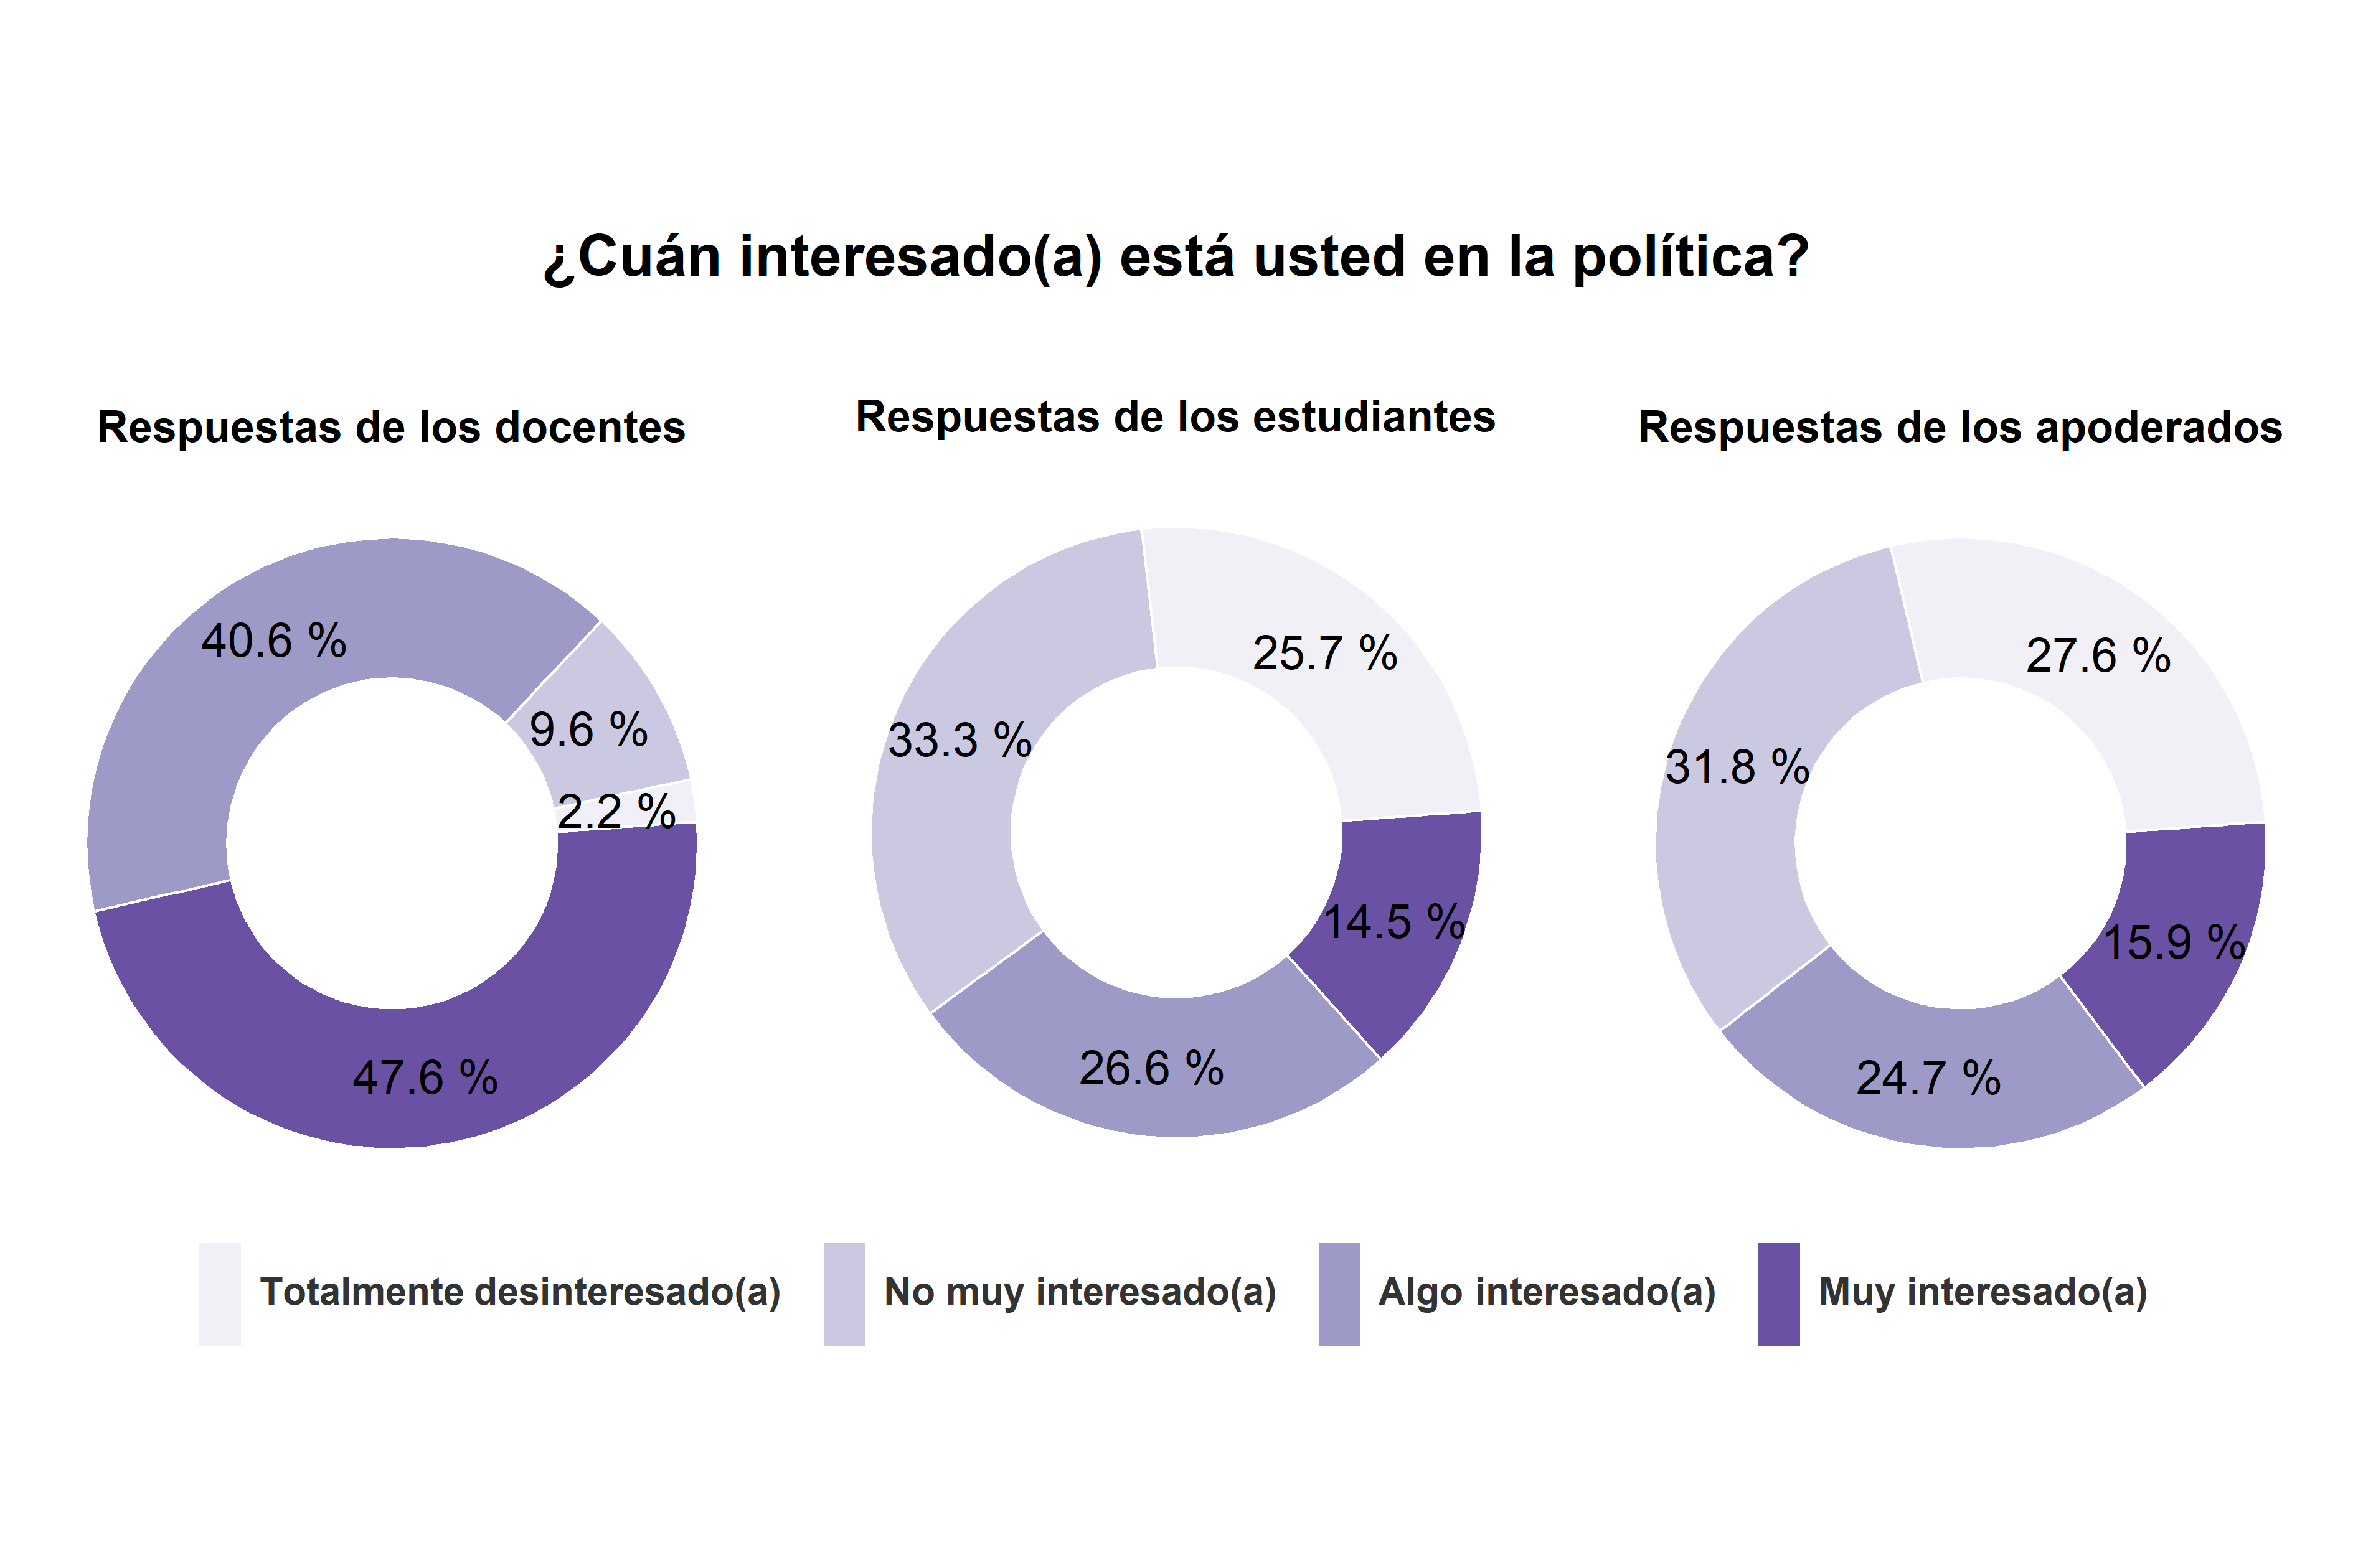
\includegraphics[width=0.8\linewidth,]{images/graph_intpol} 

}

\caption{Interés en la política}\label{fig:unnamed-chunk-37}
\end{figure}

La mayoría de los docentes está algo interesado(a) o muy interesado(a) en \emph{la política} (un 40.6\% y un 47.6\%, respectivamente). Mientras que la mayoría de los apoderados está no muy interesado(a) (un 31.8\%) o totalmente desinteresado(a) (un 27.6\%). La opinión de los estudiantes es más diversa. Un 33.3\% de los estudiantes se encuentra no muy interesado(a) en la política y un 26.6\% está algo interesado(a).

\begin{center}\rule{0.5\linewidth}{0.5pt}\end{center}

\begin{figure}[!ht]

{\centering 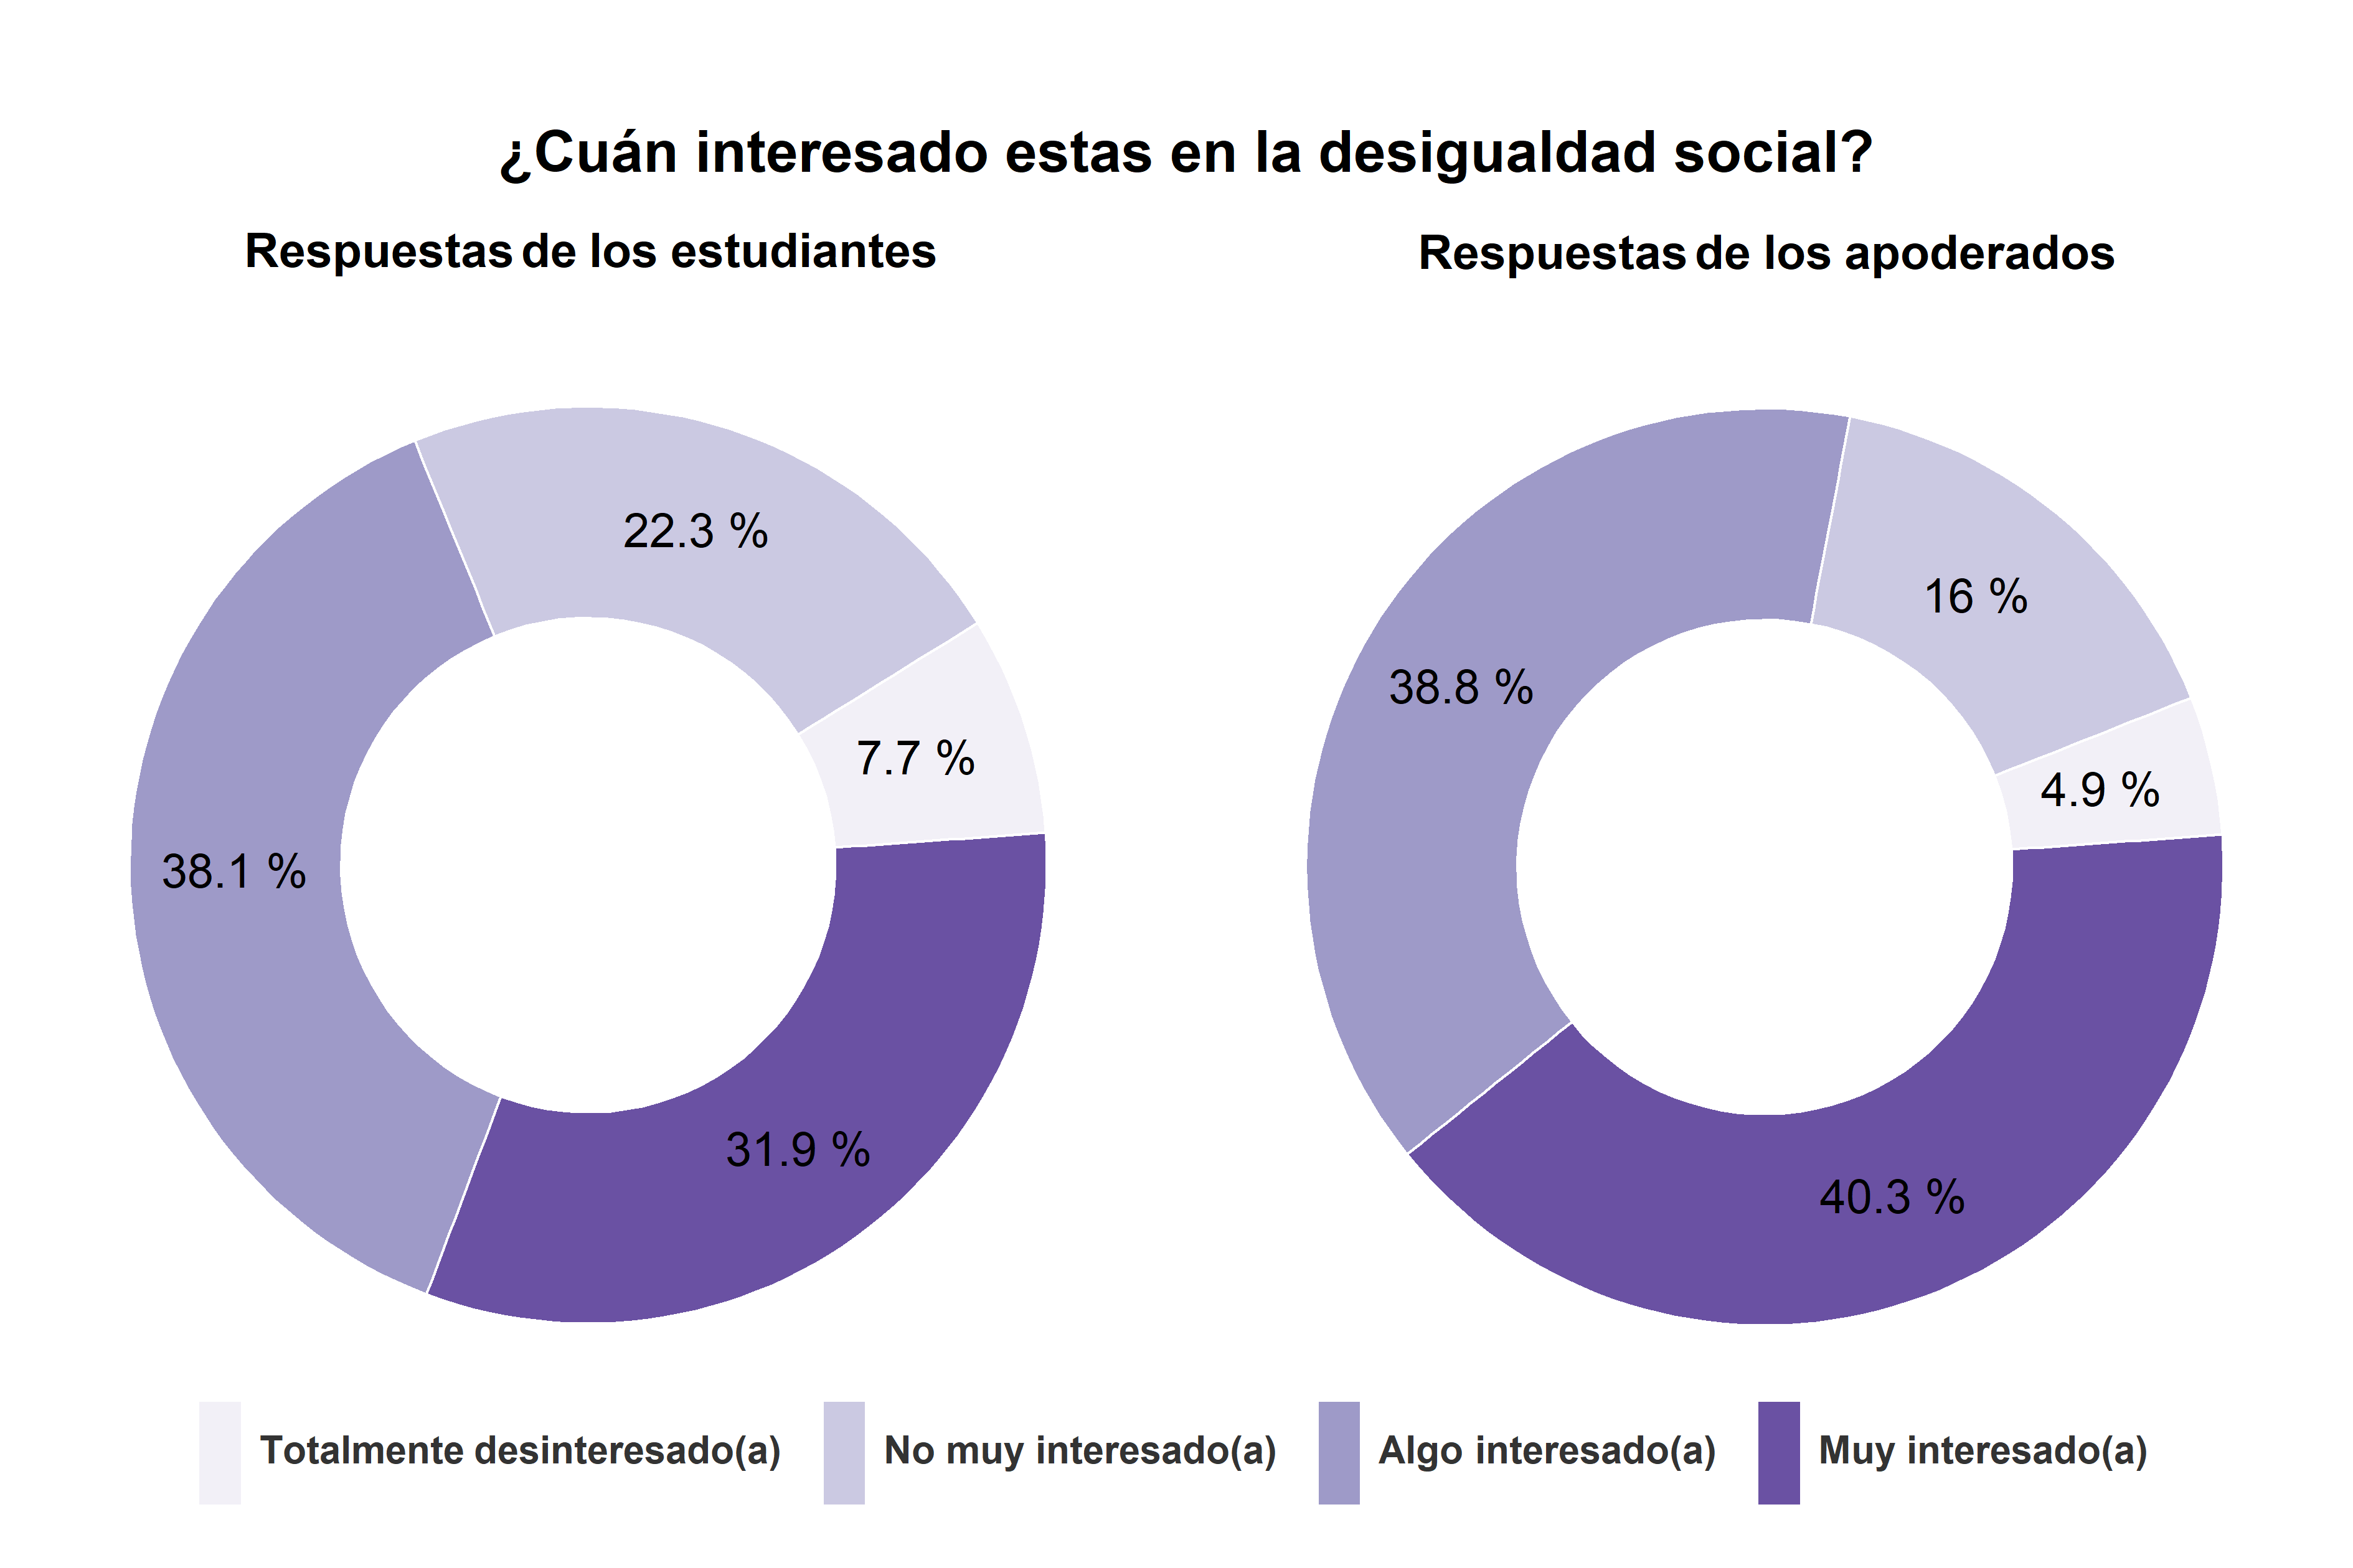
\includegraphics[width=0.8\linewidth,]{images/graph_intdes} 

}

\caption{Interés en la desigualdad social}\label{fig:unnamed-chunk-38}
\end{figure}

La mayoría de los estudiantes y apoderados señala estar algo interesado(a) (un 38.1\% y un 38.8\%, respectivamente) o muy interesado(a) en \emph{la desigualdad social} (un 31.9\% y un 40.3\%, respectivamente).

\begin{center}\rule{0.5\linewidth}{0.5pt}\end{center}

\begin{figure}[!ht]

{\centering 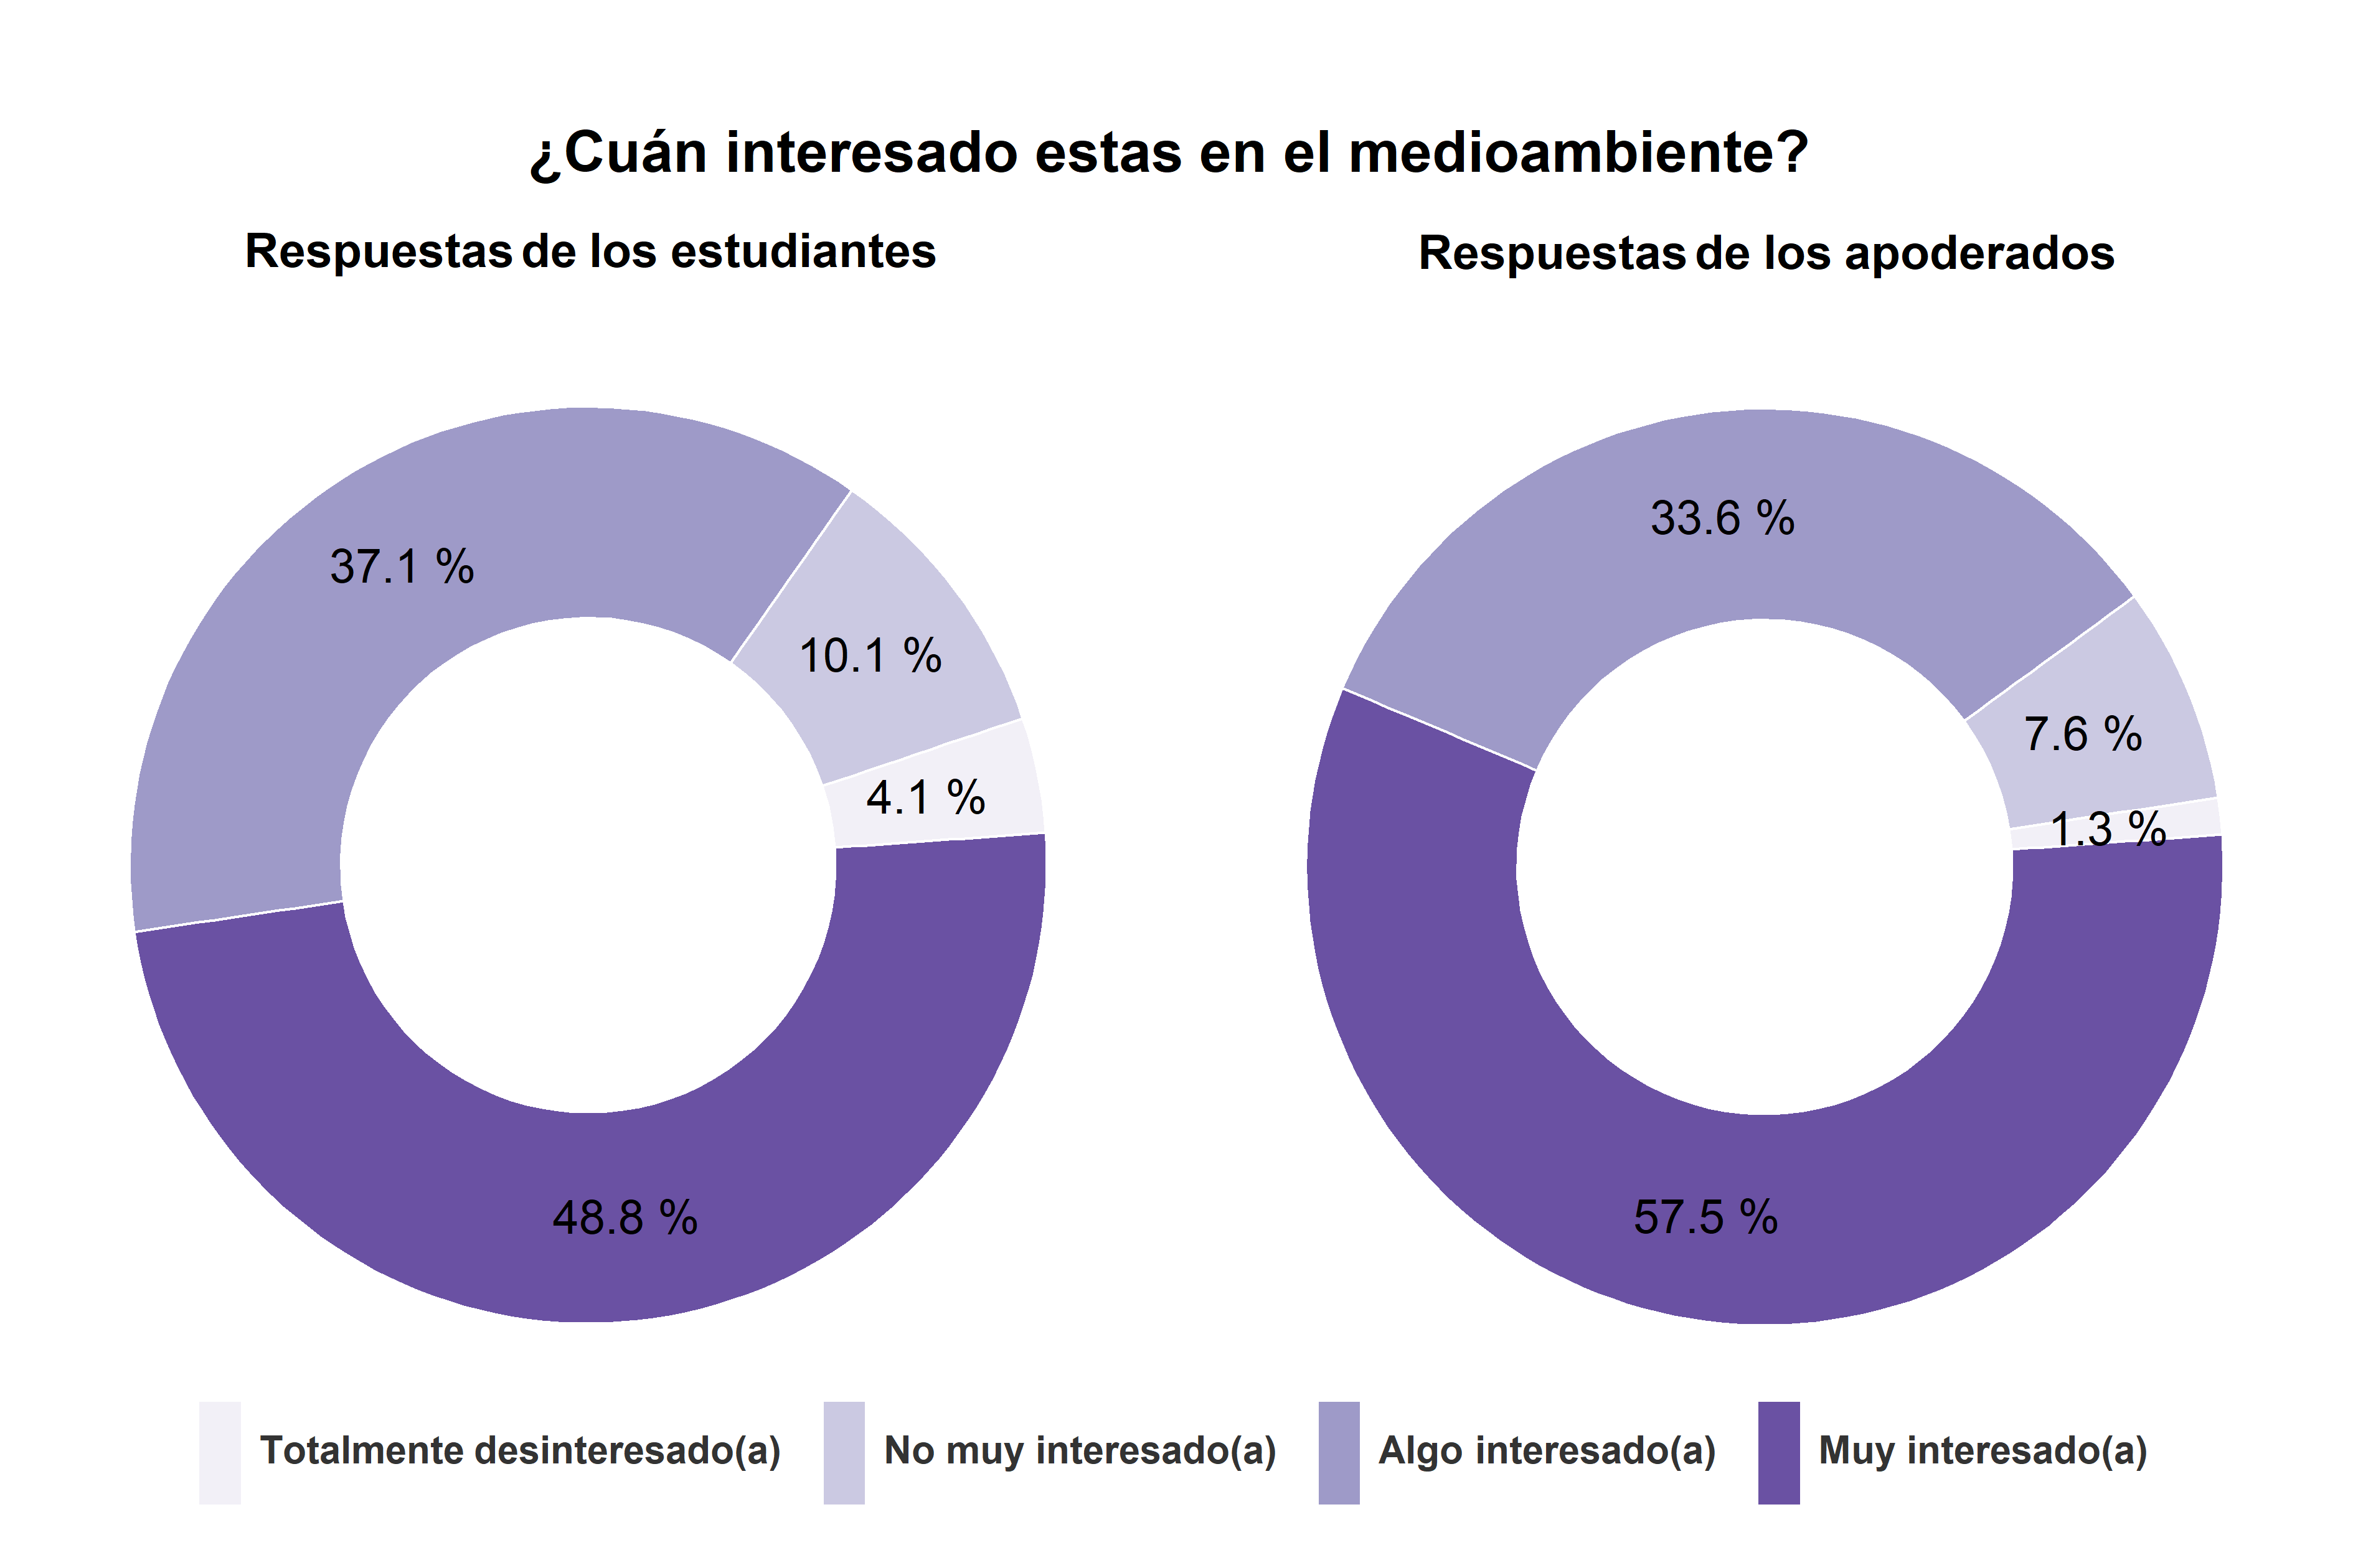
\includegraphics[width=0.8\linewidth,]{images/graph_intmed} 

}

\caption{Interés en el medioambiente}\label{fig:unnamed-chunk-39}
\end{figure}

El 48.8\% de los estudiantes y el 57.5\% de los apoderados declara estar muy interesado(a) en \emph{el medioambiente}. La mayor parte de las respuestas restantes se concentran en la opción algo interesado(a), seleccionada por el 37.1\% de los estudiantes y el 33.6\% de los apoderados.

\begin{center}\rule{0.5\linewidth}{0.5pt}\end{center}

\begin{figure}[!ht]

{\centering 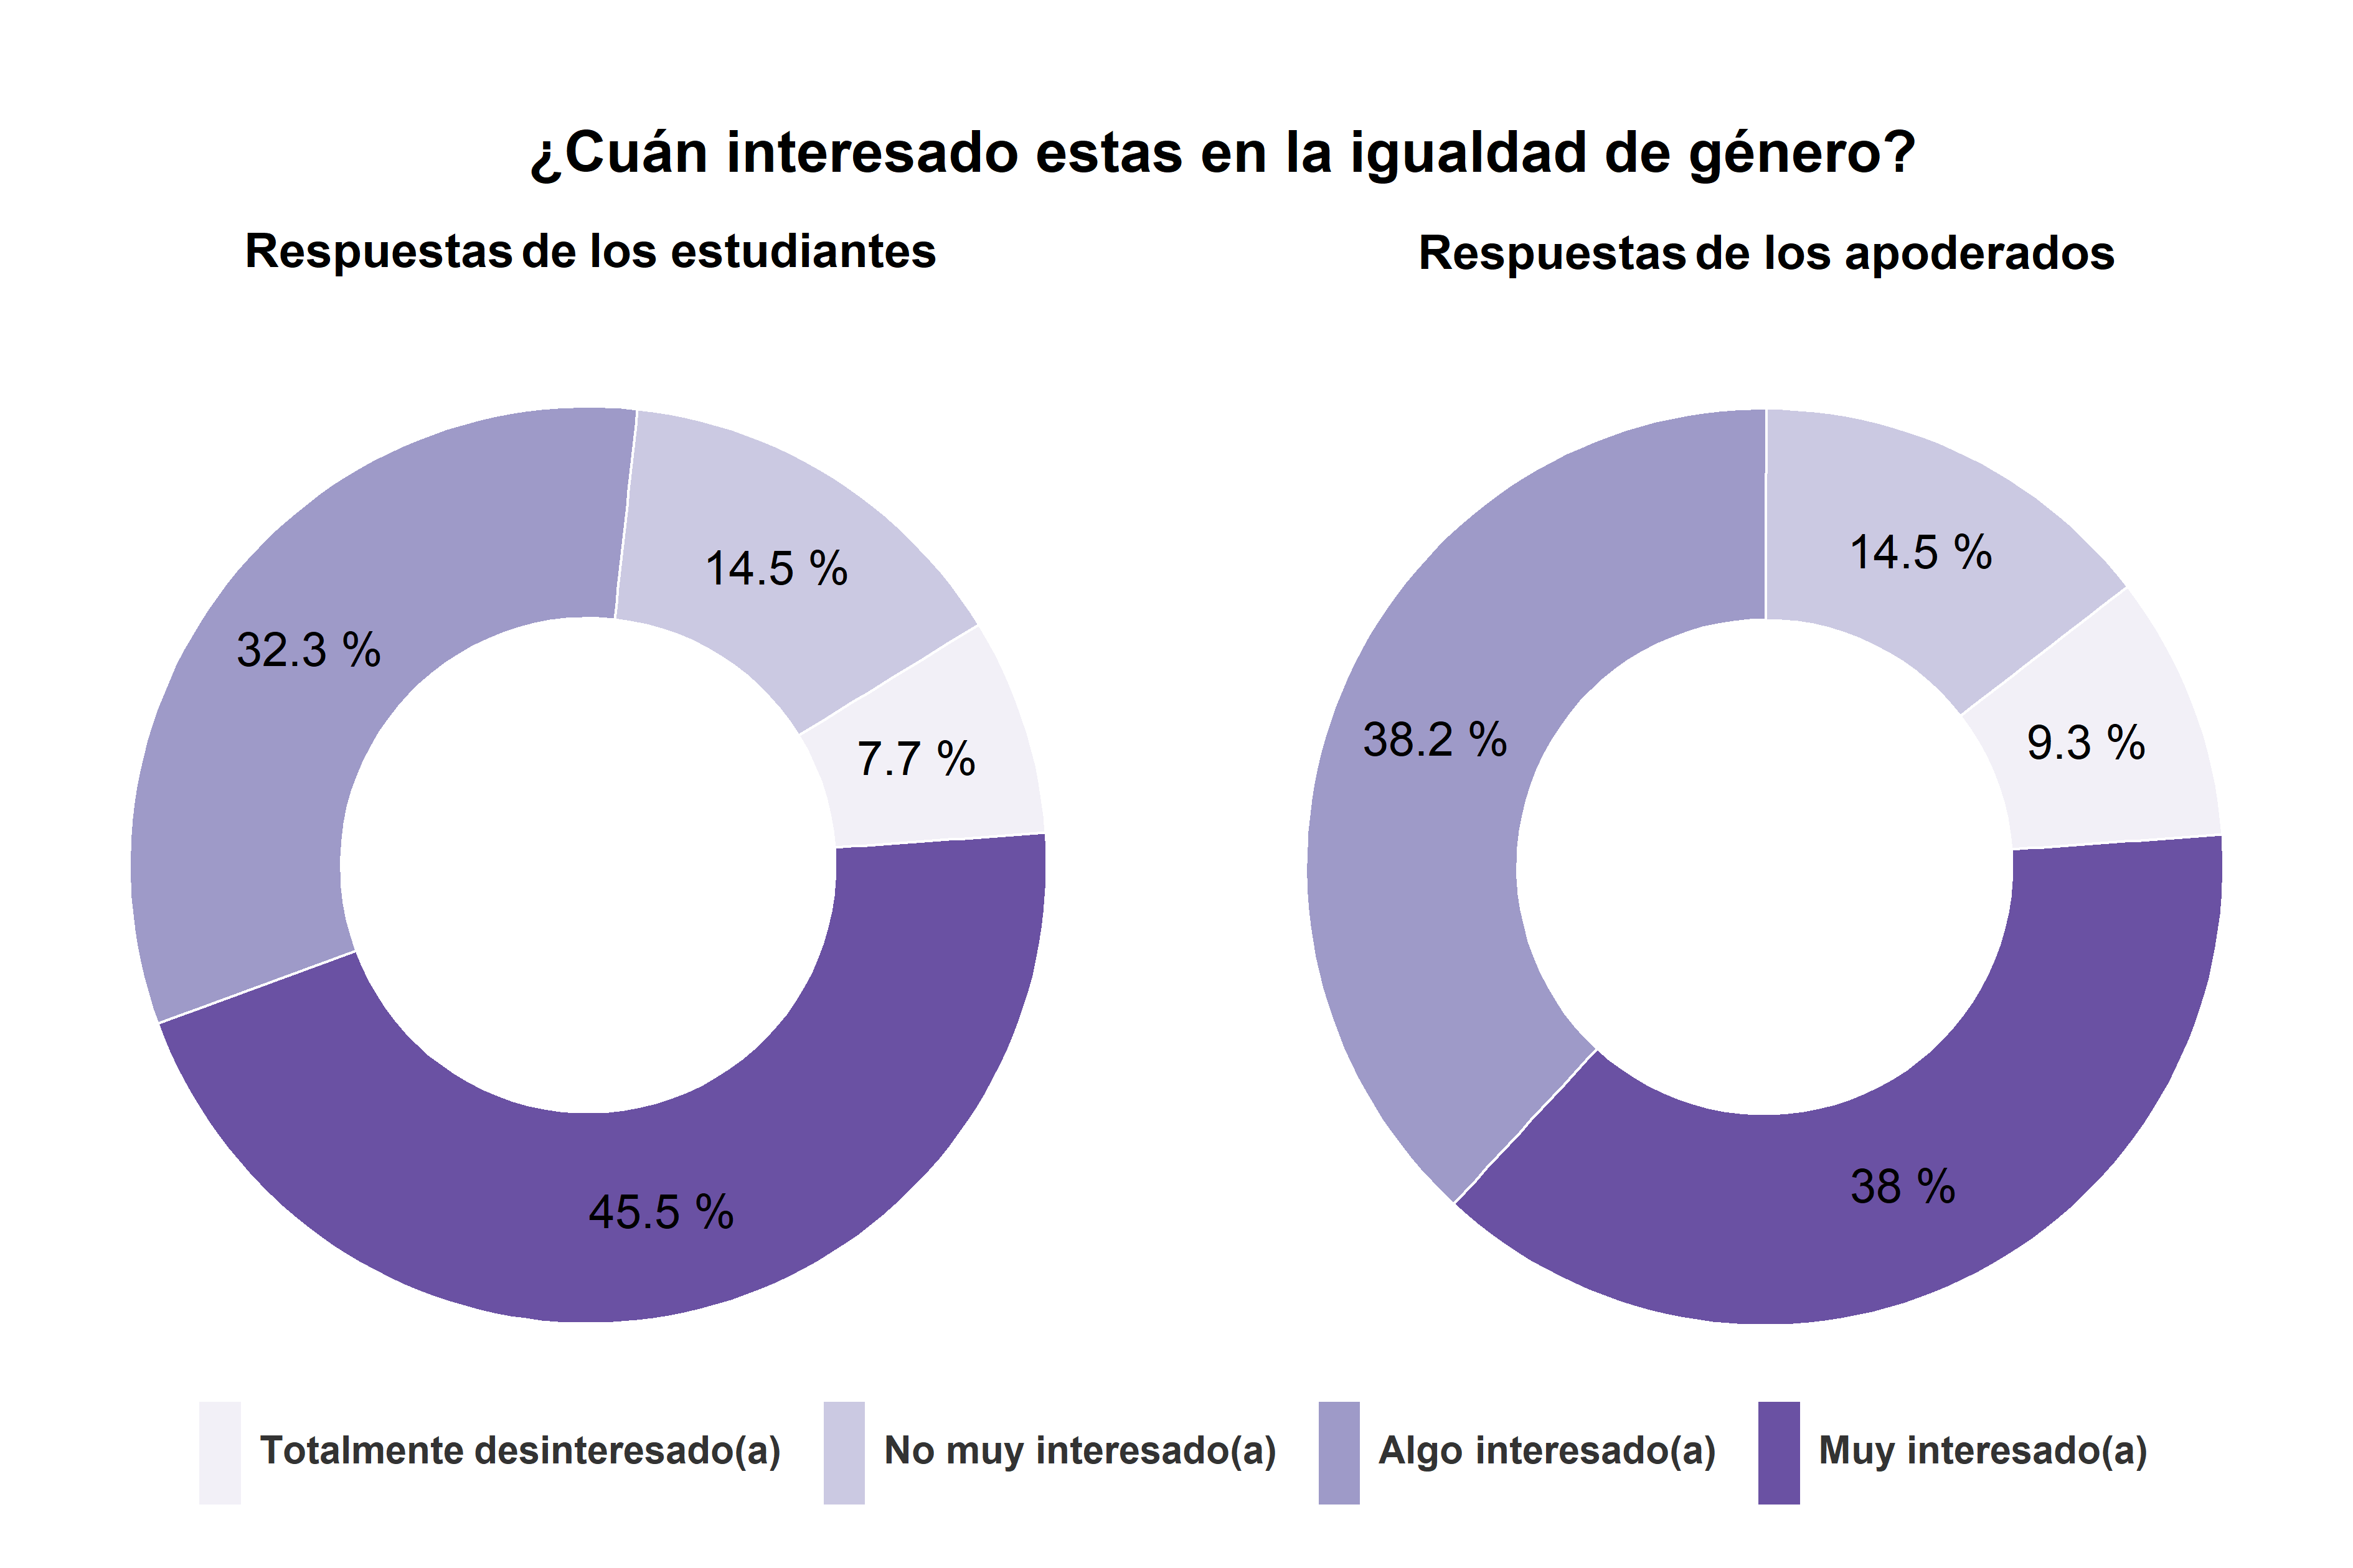
\includegraphics[width=0.8\linewidth,]{images/graph_intgen} 

}

\caption{Interés en la igualdad de género}\label{fig:unnamed-chunk-40}
\end{figure}

La mayoría de los estudiantes y apoderados está algo interesado(a) (un 32.3\% y un 38.2\%, respectivamente) o muy interesado(a) en \emph{la igualdad de género} (un 45.5\% y un 38\%, respectivamente).

\begin{center}\rule{0.5\linewidth}{0.5pt}\end{center}

\hypertarget{satisfacciuxf3n-con-la-democracia-y-actitudes-autoritarias}{%
\section{Satisfacción con la democracia y actitudes autoritarias}\label{satisfacciuxf3n-con-la-democracia-y-actitudes-autoritarias}}

\begin{center}\rule{0.5\linewidth}{0.5pt}\end{center}

\begin{figure}[!ht]

{\centering 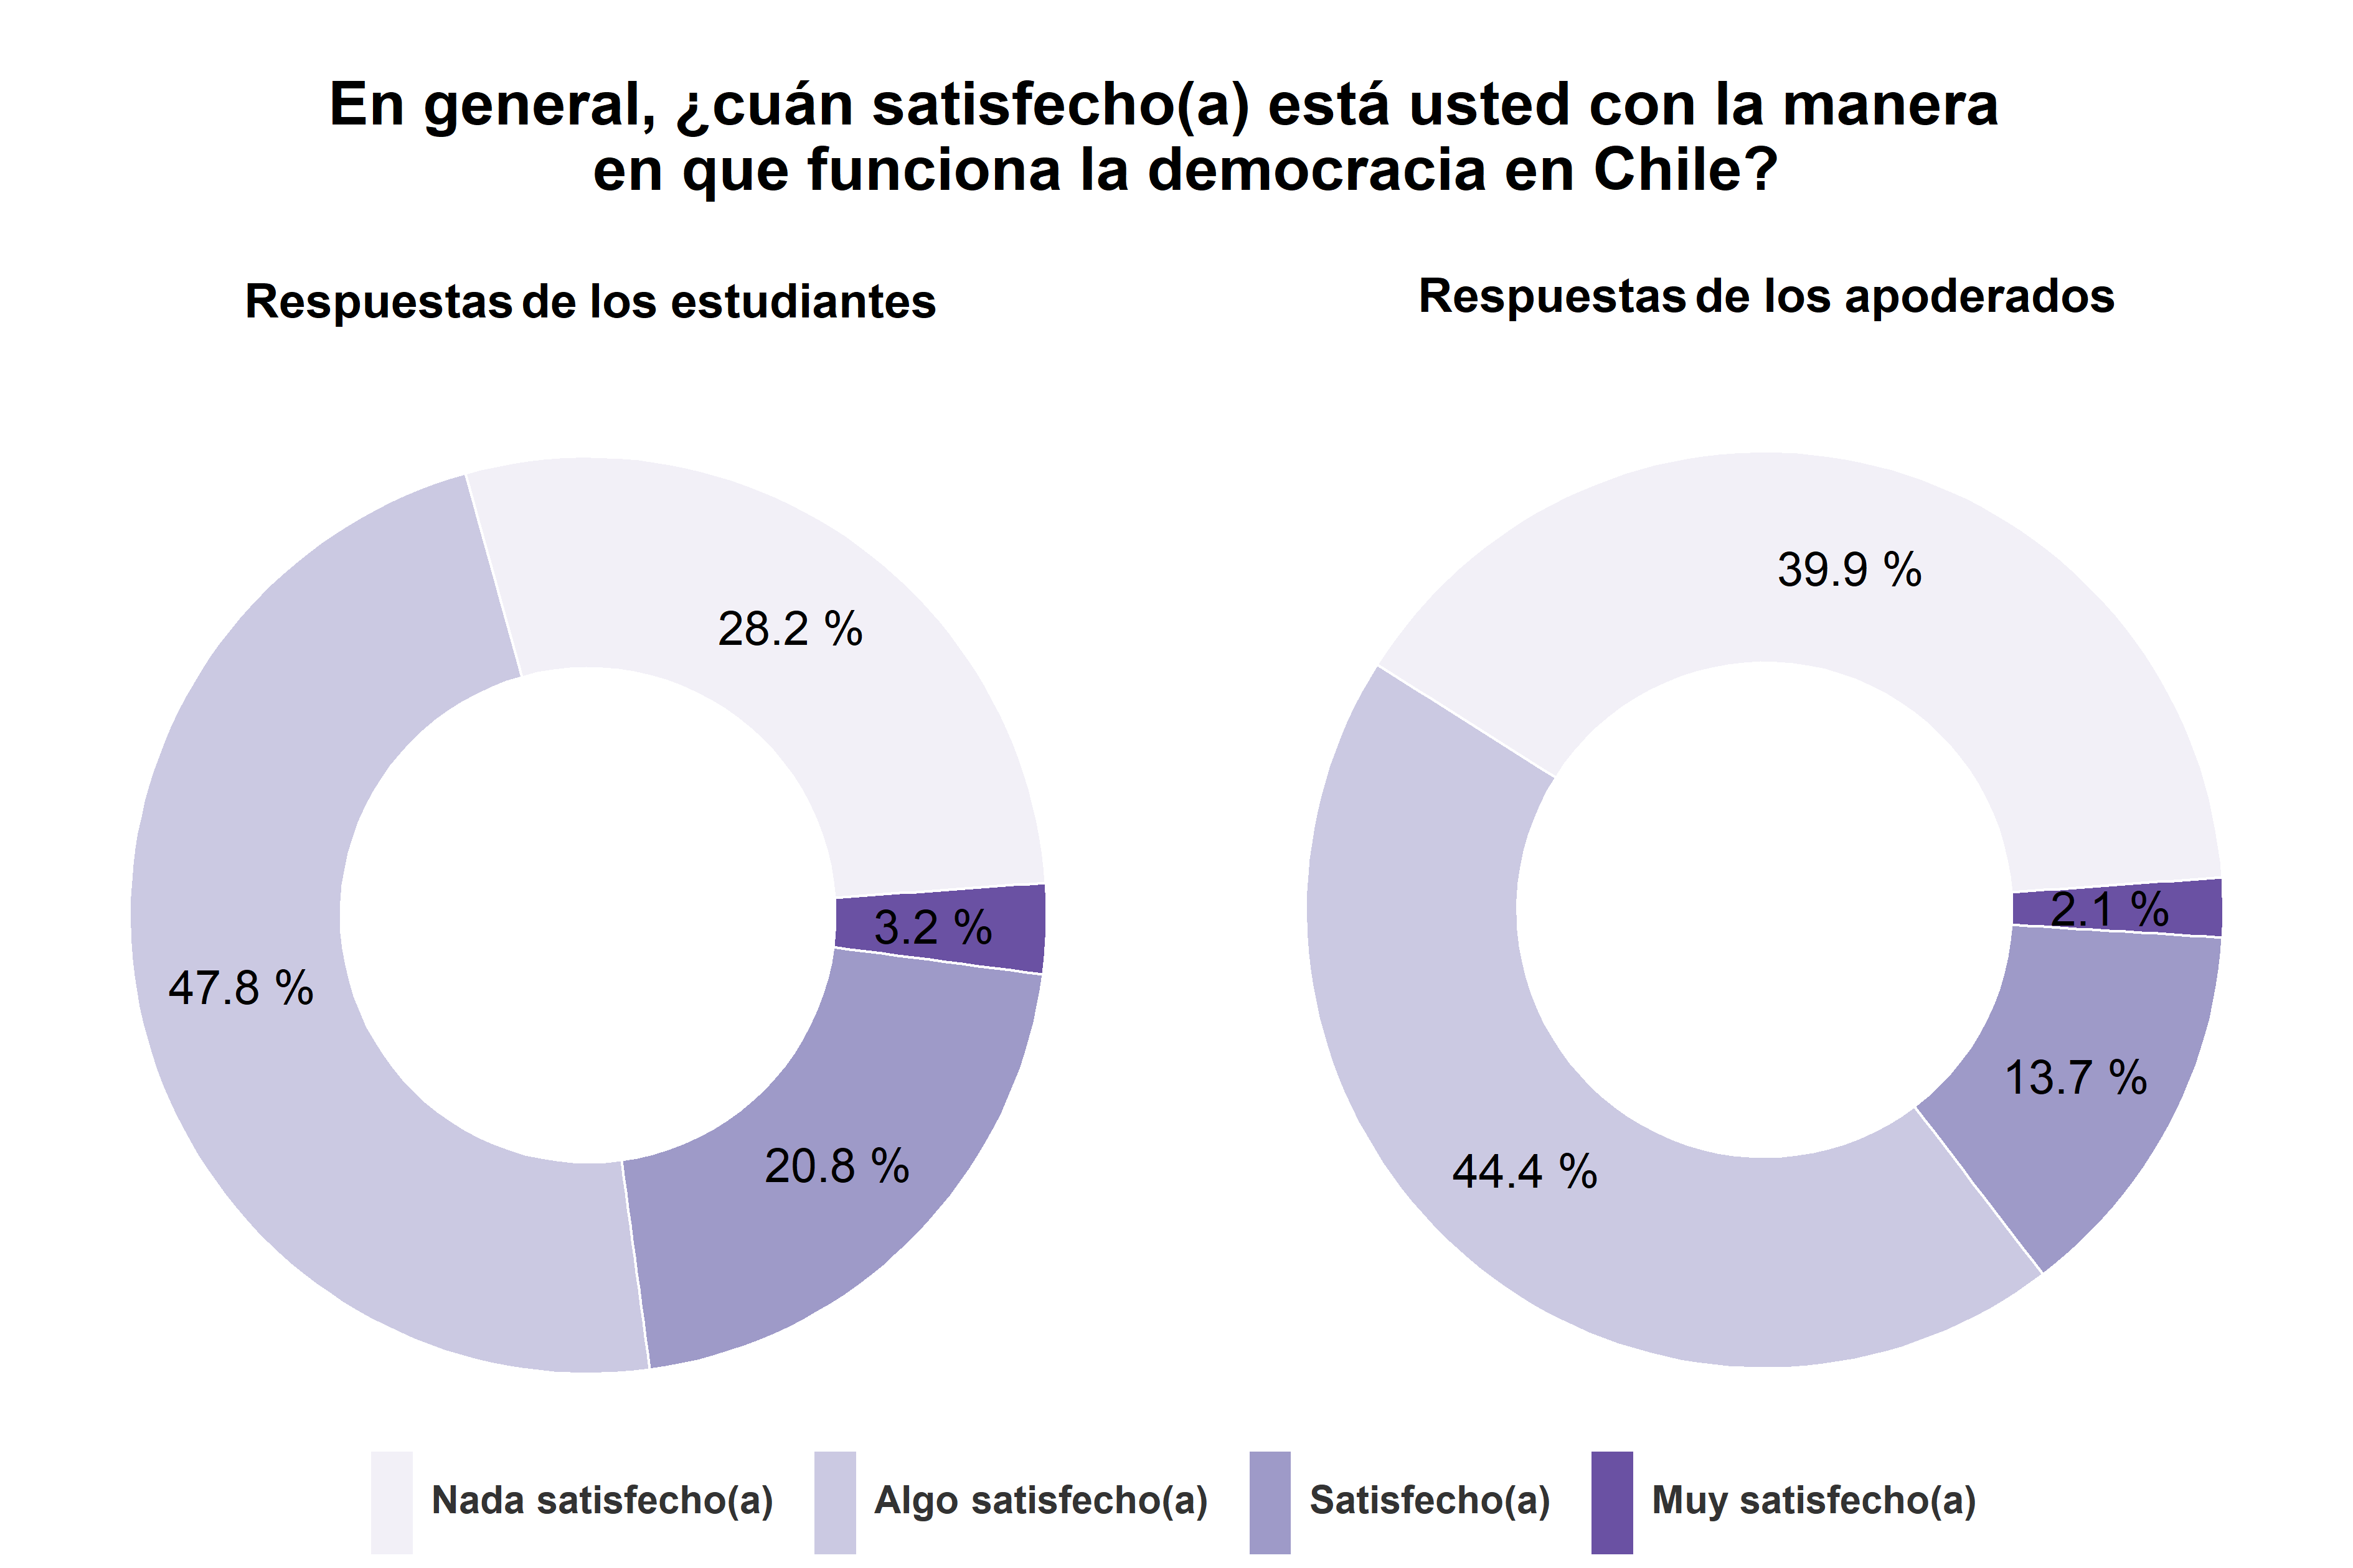
\includegraphics[width=0.8\linewidth,]{images/graph_dem} 

}

\caption{Satisfacción con la democracia}\label{fig:unnamed-chunk-41}
\end{figure}

La mayoría de los estudiantes y apoderados se encuentra nada satisfecho(a) (un 30.8\% y un 38.2\%, respectivamente) o algo satisfecho(a) con \emph{la manera en que funciona la democracia en Chile} (un 48.5\% y un 45.7\%, respectivamente).

\begin{center}\rule{0.5\linewidth}{0.5pt}\end{center}

\begin{figure}[!ht]

{\centering 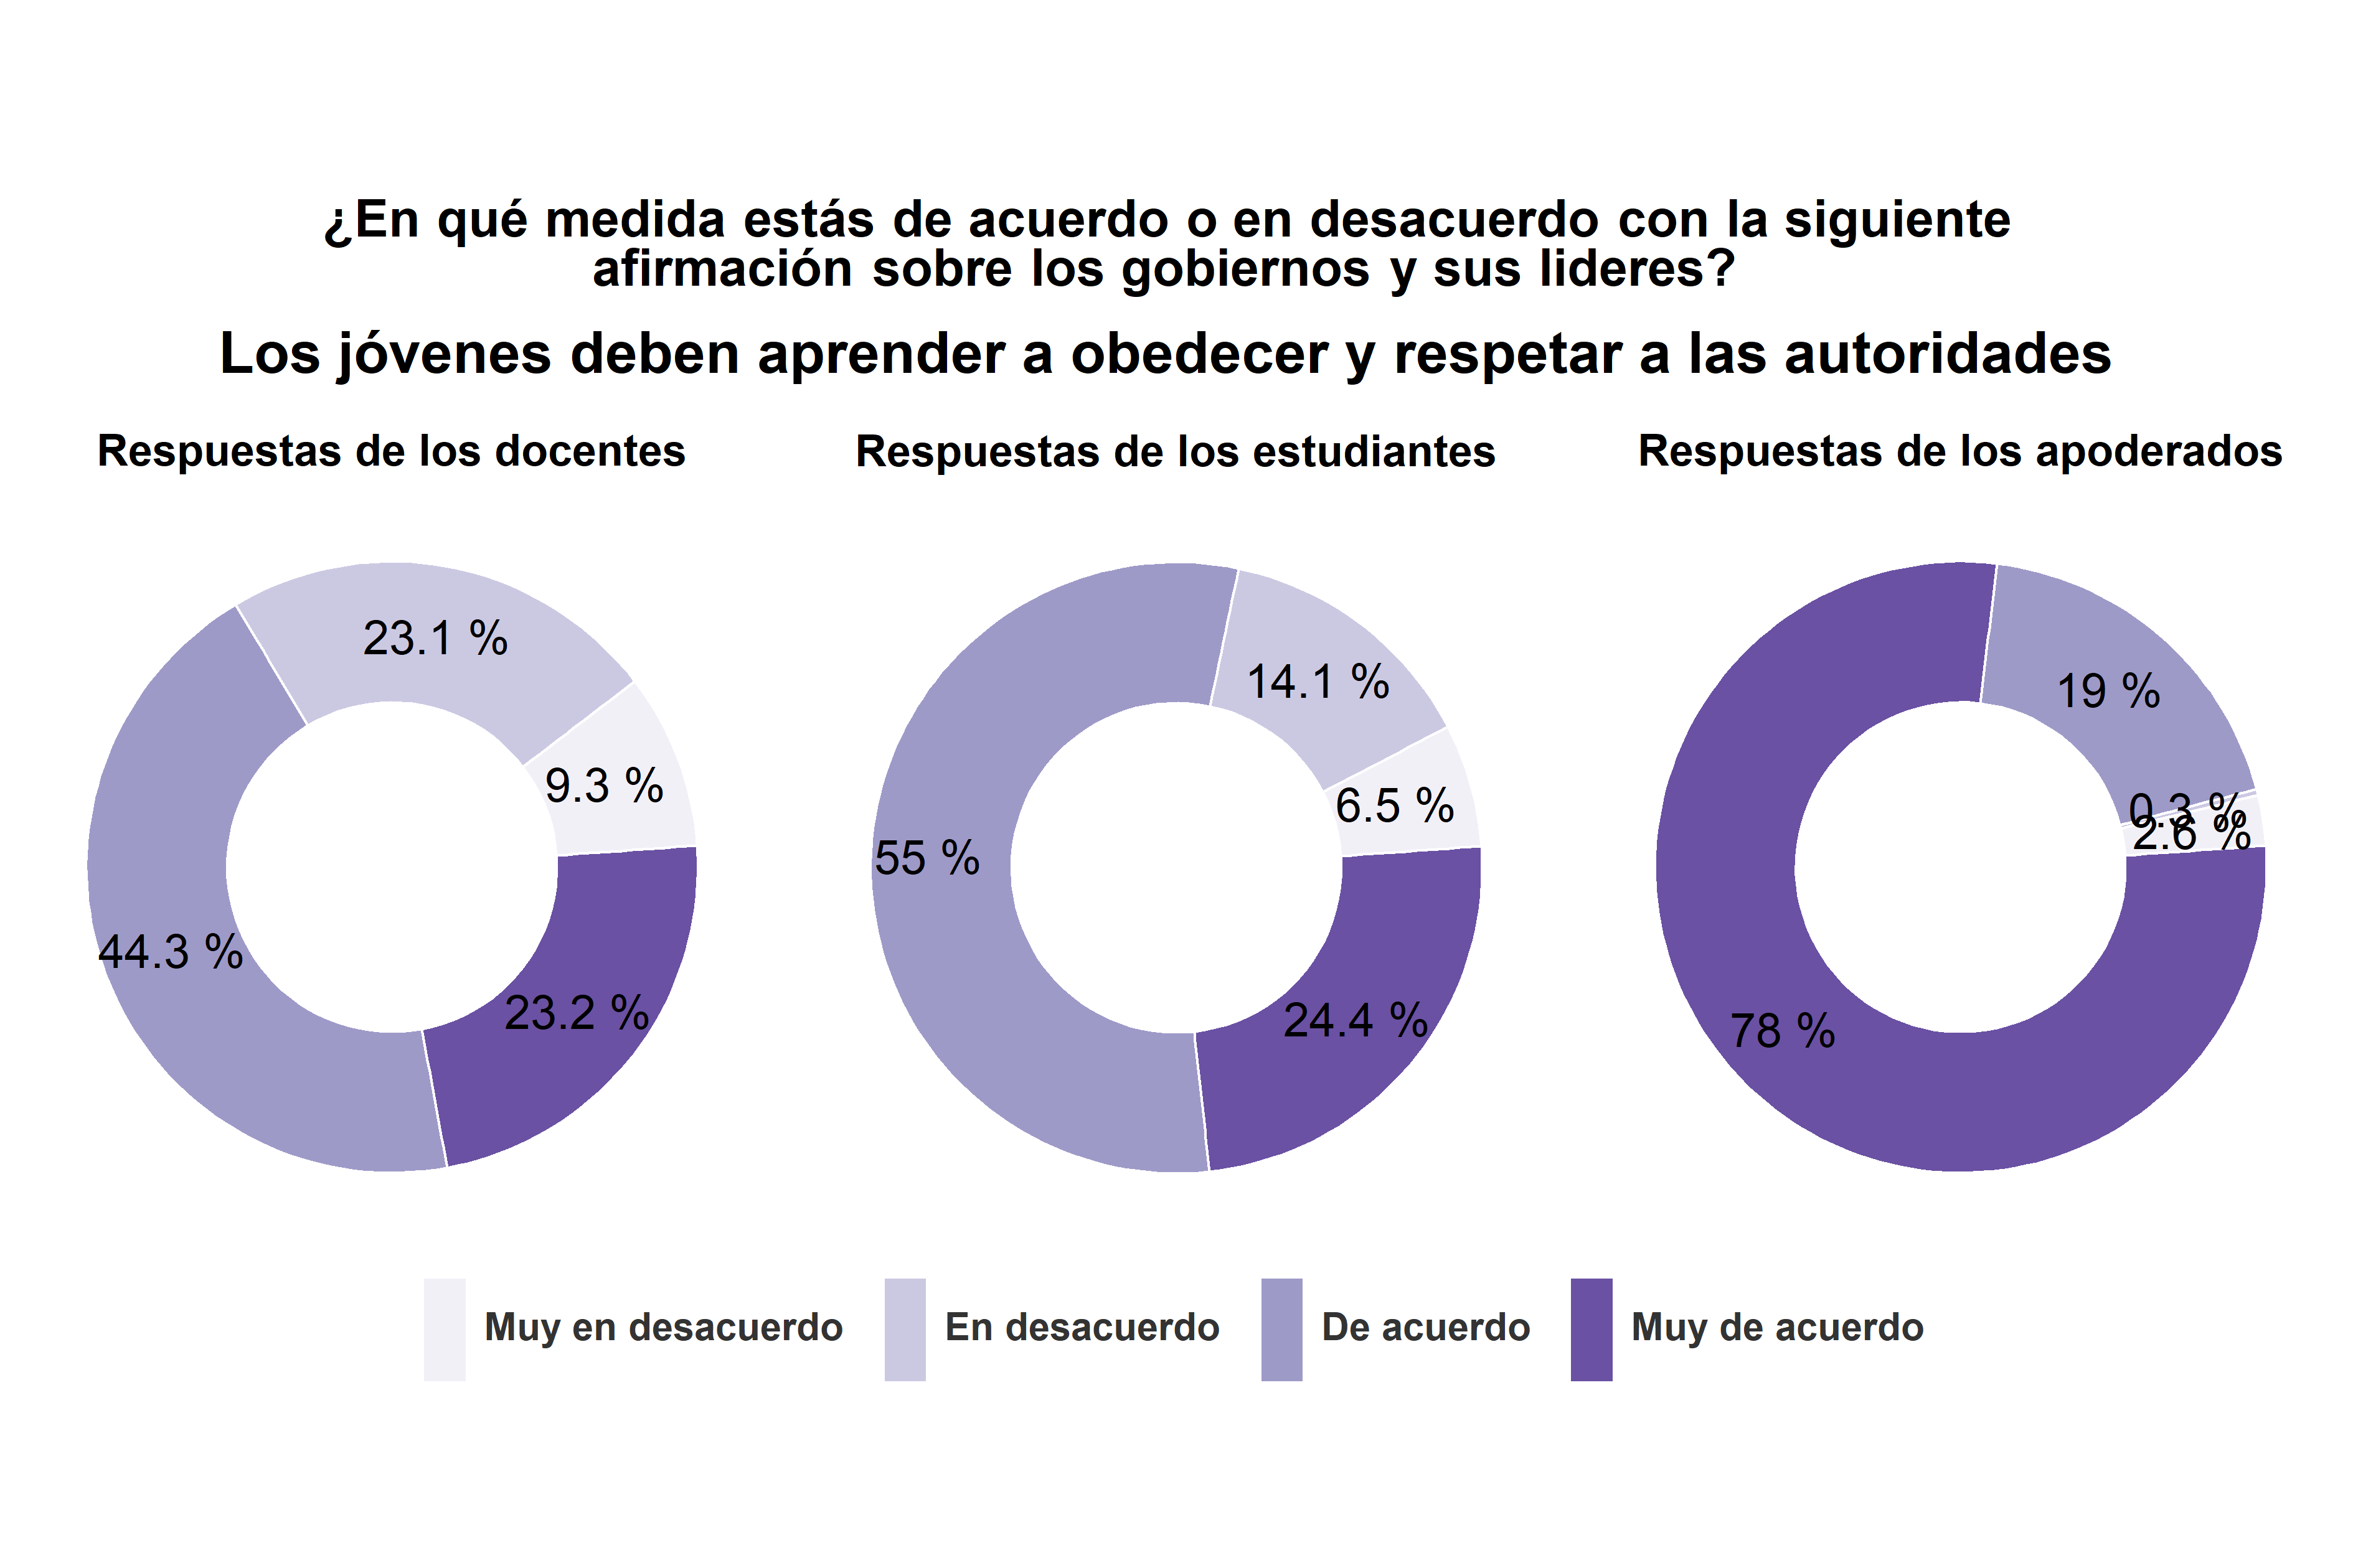
\includegraphics[width=0.8\linewidth,]{images/graph_aut1} 

}

\caption{Los jóvenes deben aprender a obedecer a las autoridades}\label{fig:unnamed-chunk-42}
\end{figure}

La mayoría de los apoderados está muy de acuerdo con que \emph{los jóvenes deben aprender a obedecer y respetar a las autoridades} (un 78\%). Mientras que la mayor parte de los docentes y de los estudiantes se encuentra de acuerdo con esta afirmación (un 44.3\% y un 55\%, respectivamente).

\begin{center}\rule{0.5\linewidth}{0.5pt}\end{center}

\begin{figure}[!ht]

{\centering 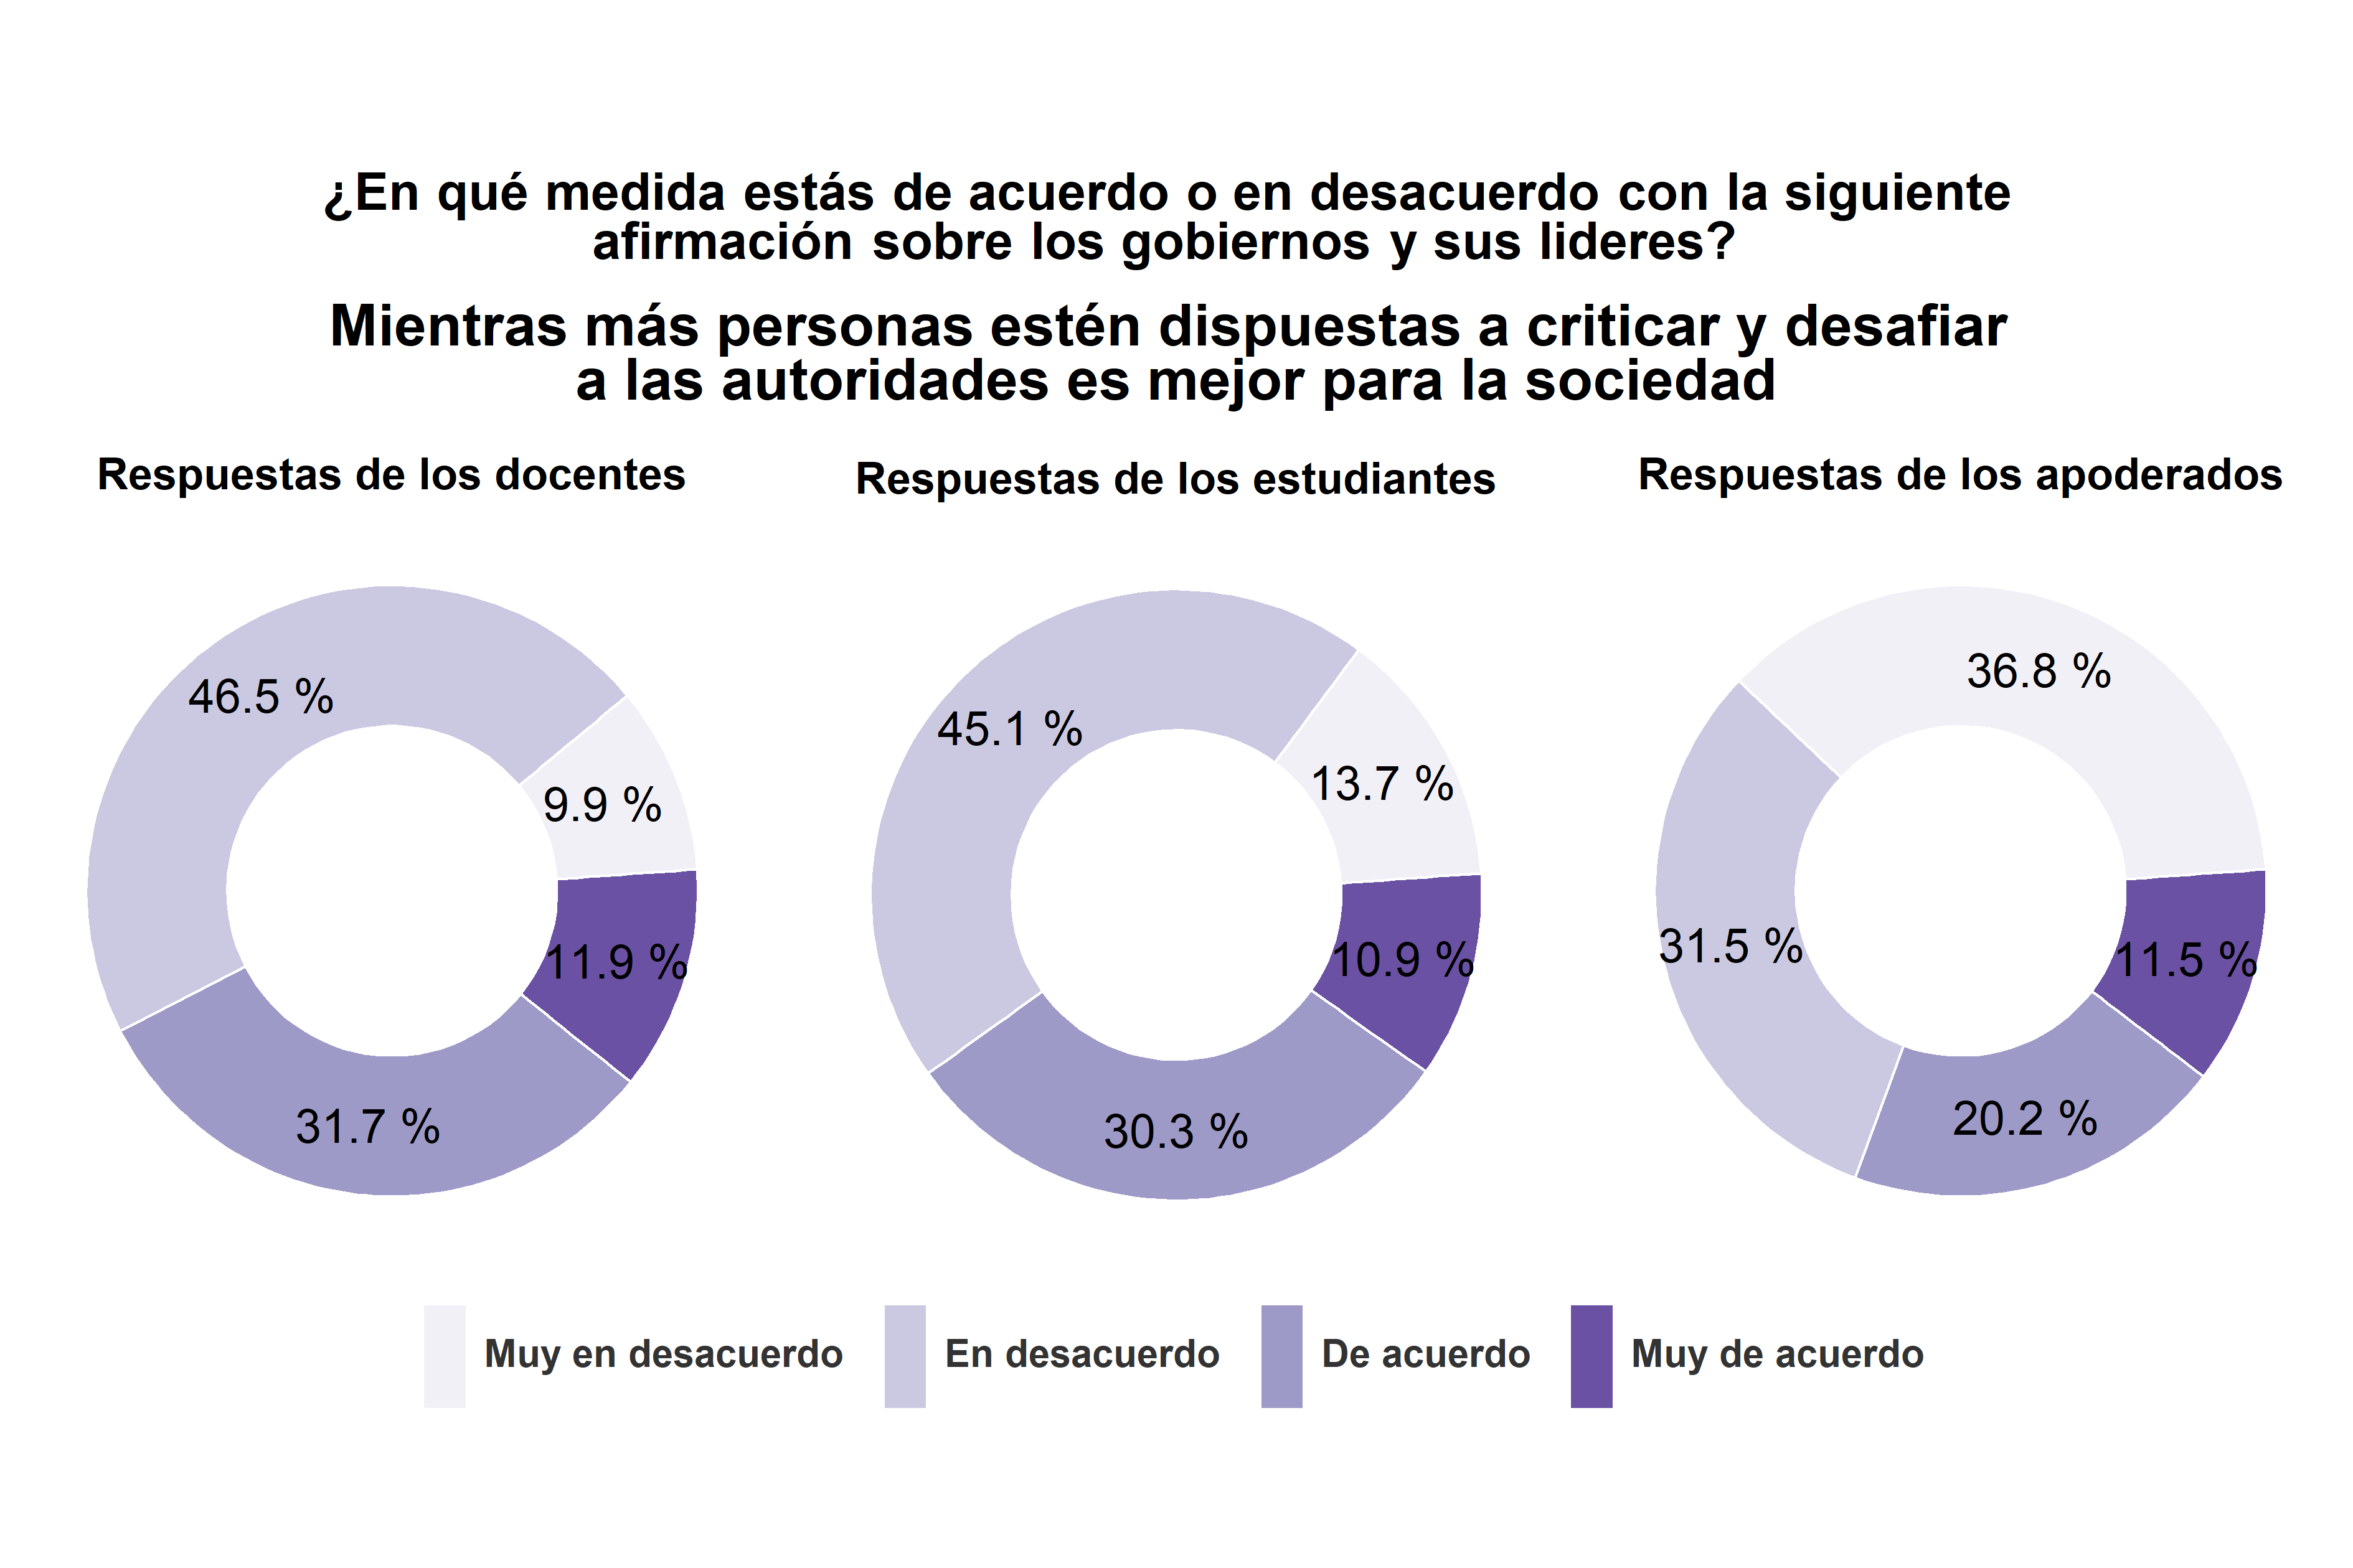
\includegraphics[width=0.8\linewidth,]{images/graph_aut2} 

}

\caption{Criticar y desafiar a las autoridades es mejor para la sociedad}\label{fig:unnamed-chunk-43}
\end{figure}

La mayor parte de los docentes y estudiantes se encuentra en desacuerdo con que \emph{mientras más personas estén dispuestas a criticar y desafiar a las autoridades es mejor para la sociedad} (el 48.3\% y el 45.4\%, respectivamente), pero en ambos grupos hay un sector numeroso que está de acuerdo con la afirmación (el 26.3\% y el 29.5\%, respectivamente). Por su parte, la mayoría de los apoderados se encuentra muy en desacuerdo (el 39.8\%) o en desacuerdo (el 31.3\%) con la afirmación.

\begin{center}\rule{0.5\linewidth}{0.5pt}\end{center}

\begin{figure}[!ht]

{\centering 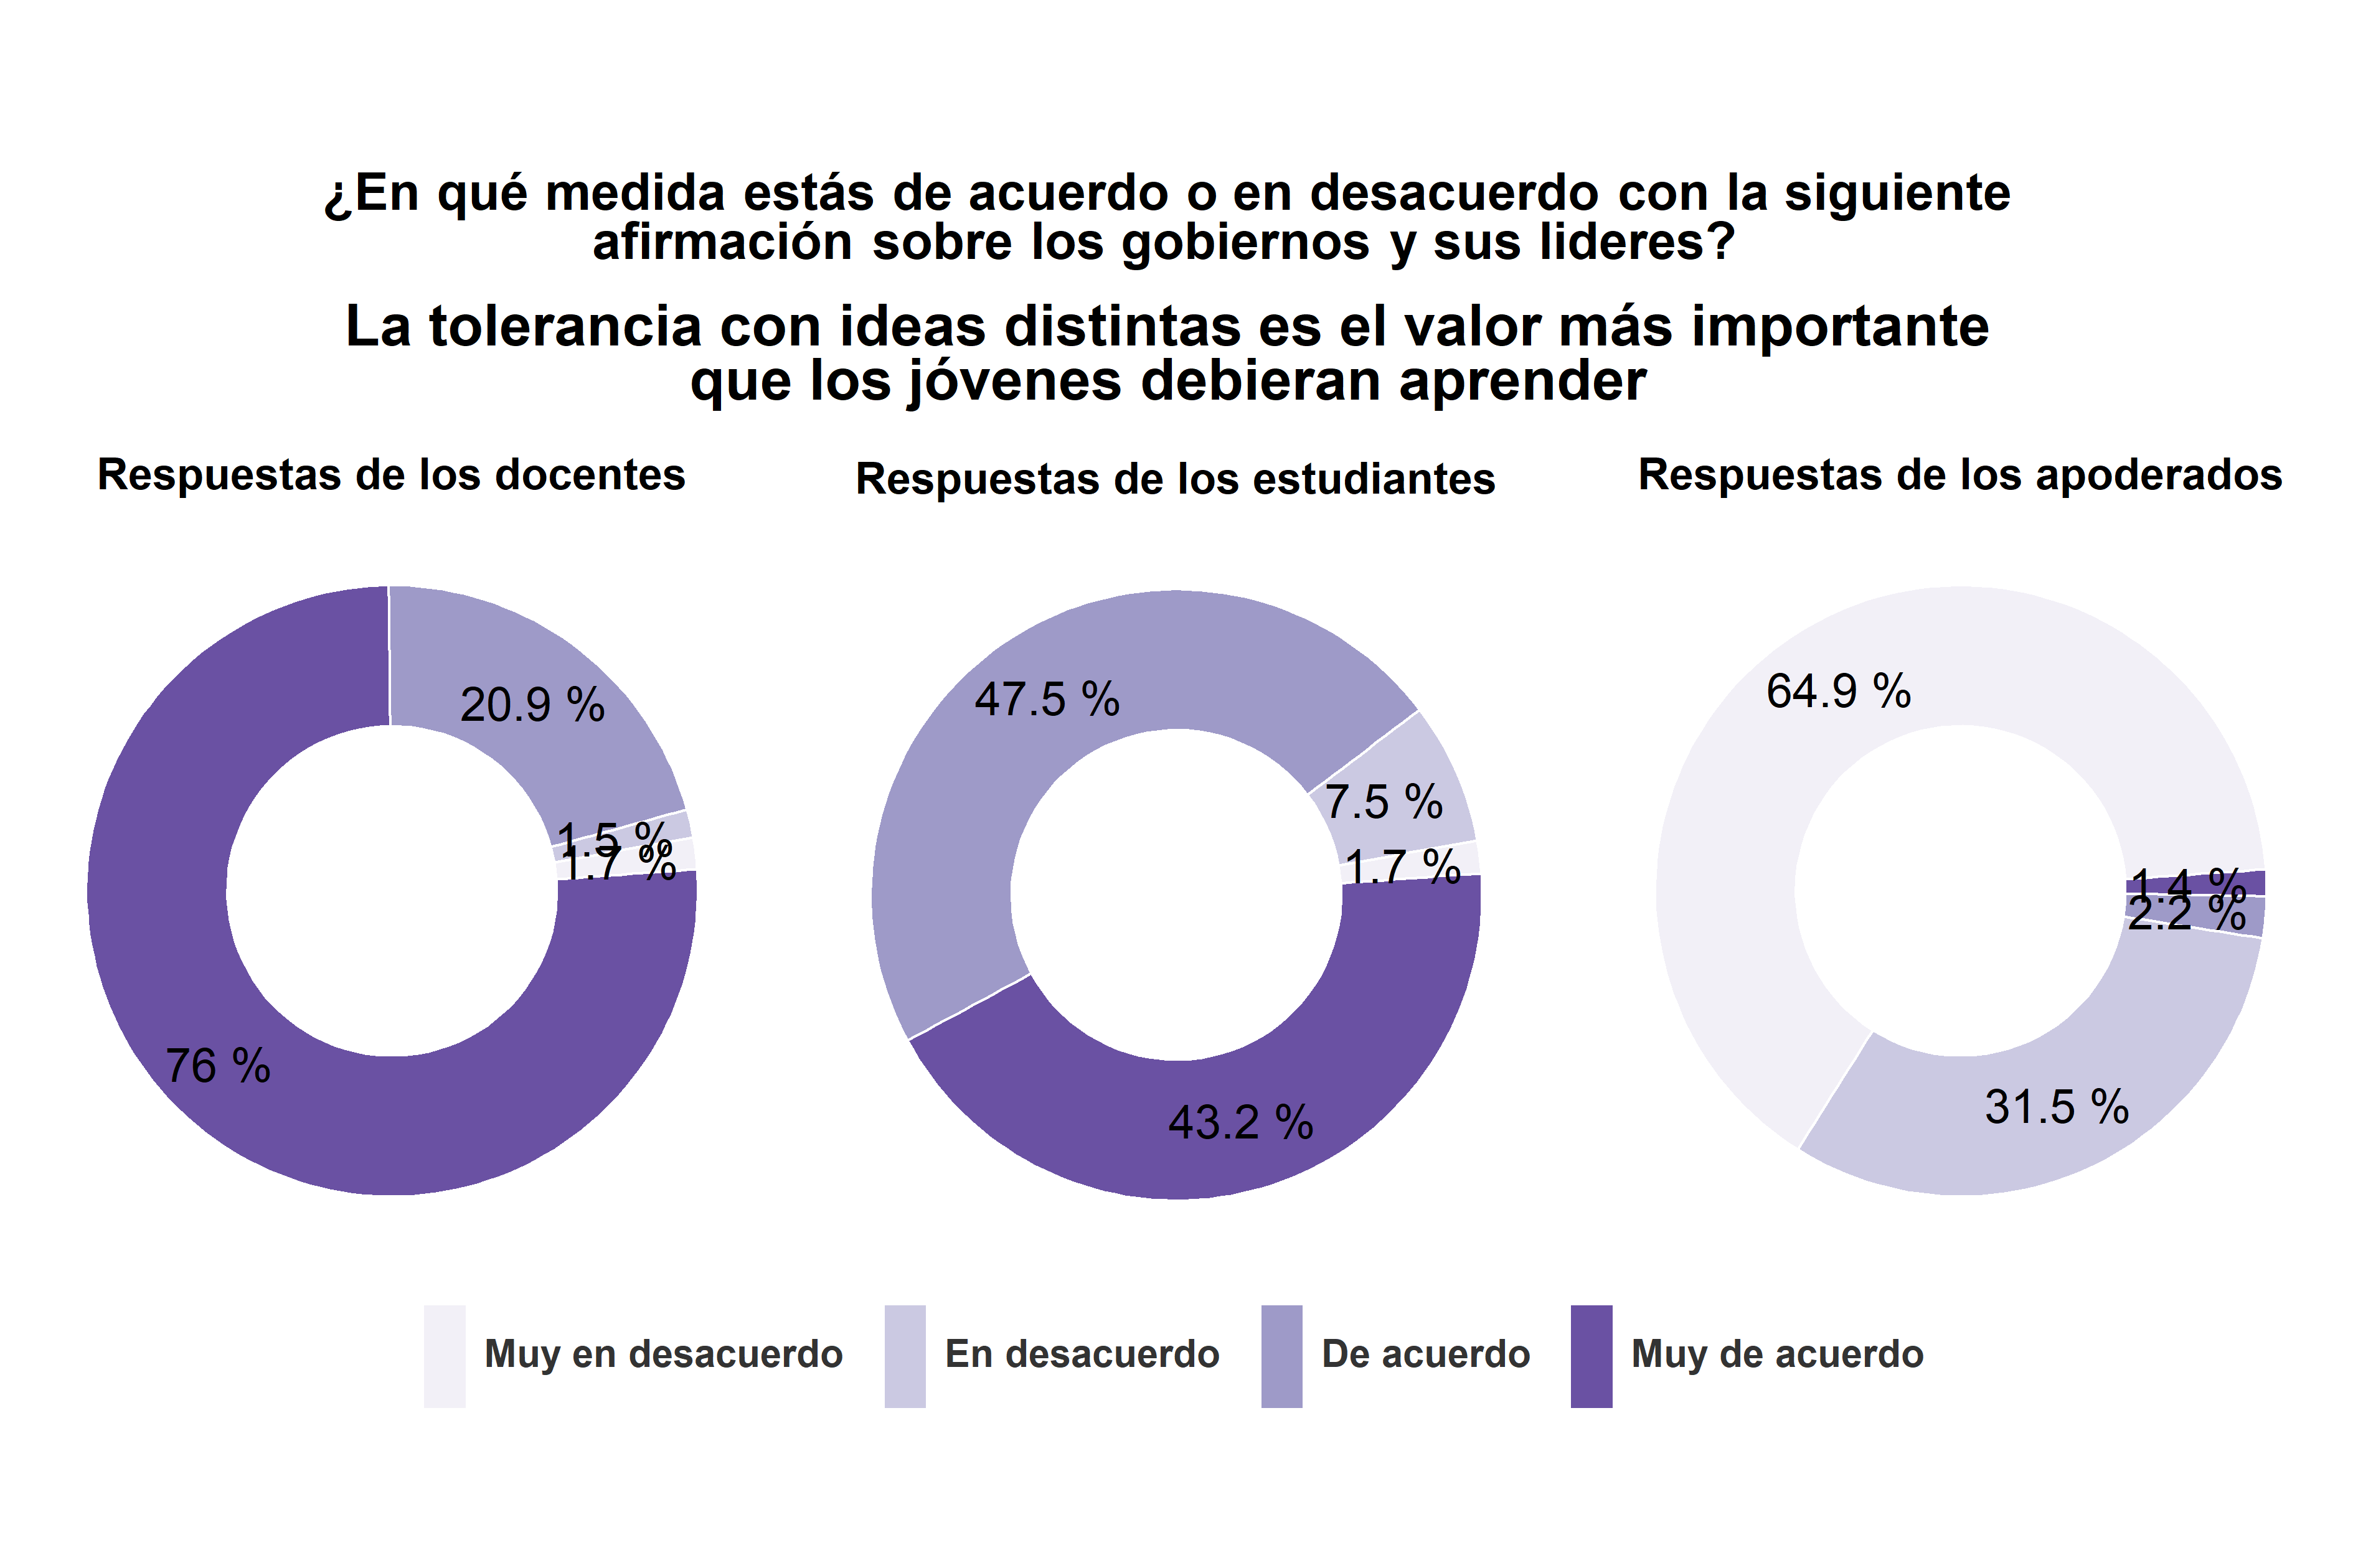
\includegraphics[width=0.8\linewidth,]{images/graph_aut3} 

}

\caption{Tolerar ideas distintas es el valor más importante que debieran aprender}\label{fig:unnamed-chunk-44}
\end{figure}

La mayoría de los docentes está muy de acuerdo con que \emph{la tolerancia con ideas distintas es el valor más importante que los jóvenes debieran aprender} (un 76\%) y la mayor parte de los estudiantes se encuentra de acuerdo (un 47.5\%) o muy de acuerdo (un 43.2\%) con la afirmación. Mientras que la mayoría de los apoderados está muy en desacuerdo (un 64.9\%) o en desacuerdo con la afirmación (un 31.5\%).

\begin{center}\rule{0.5\linewidth}{0.5pt}\end{center}

\begin{figure}[!ht]

{\centering 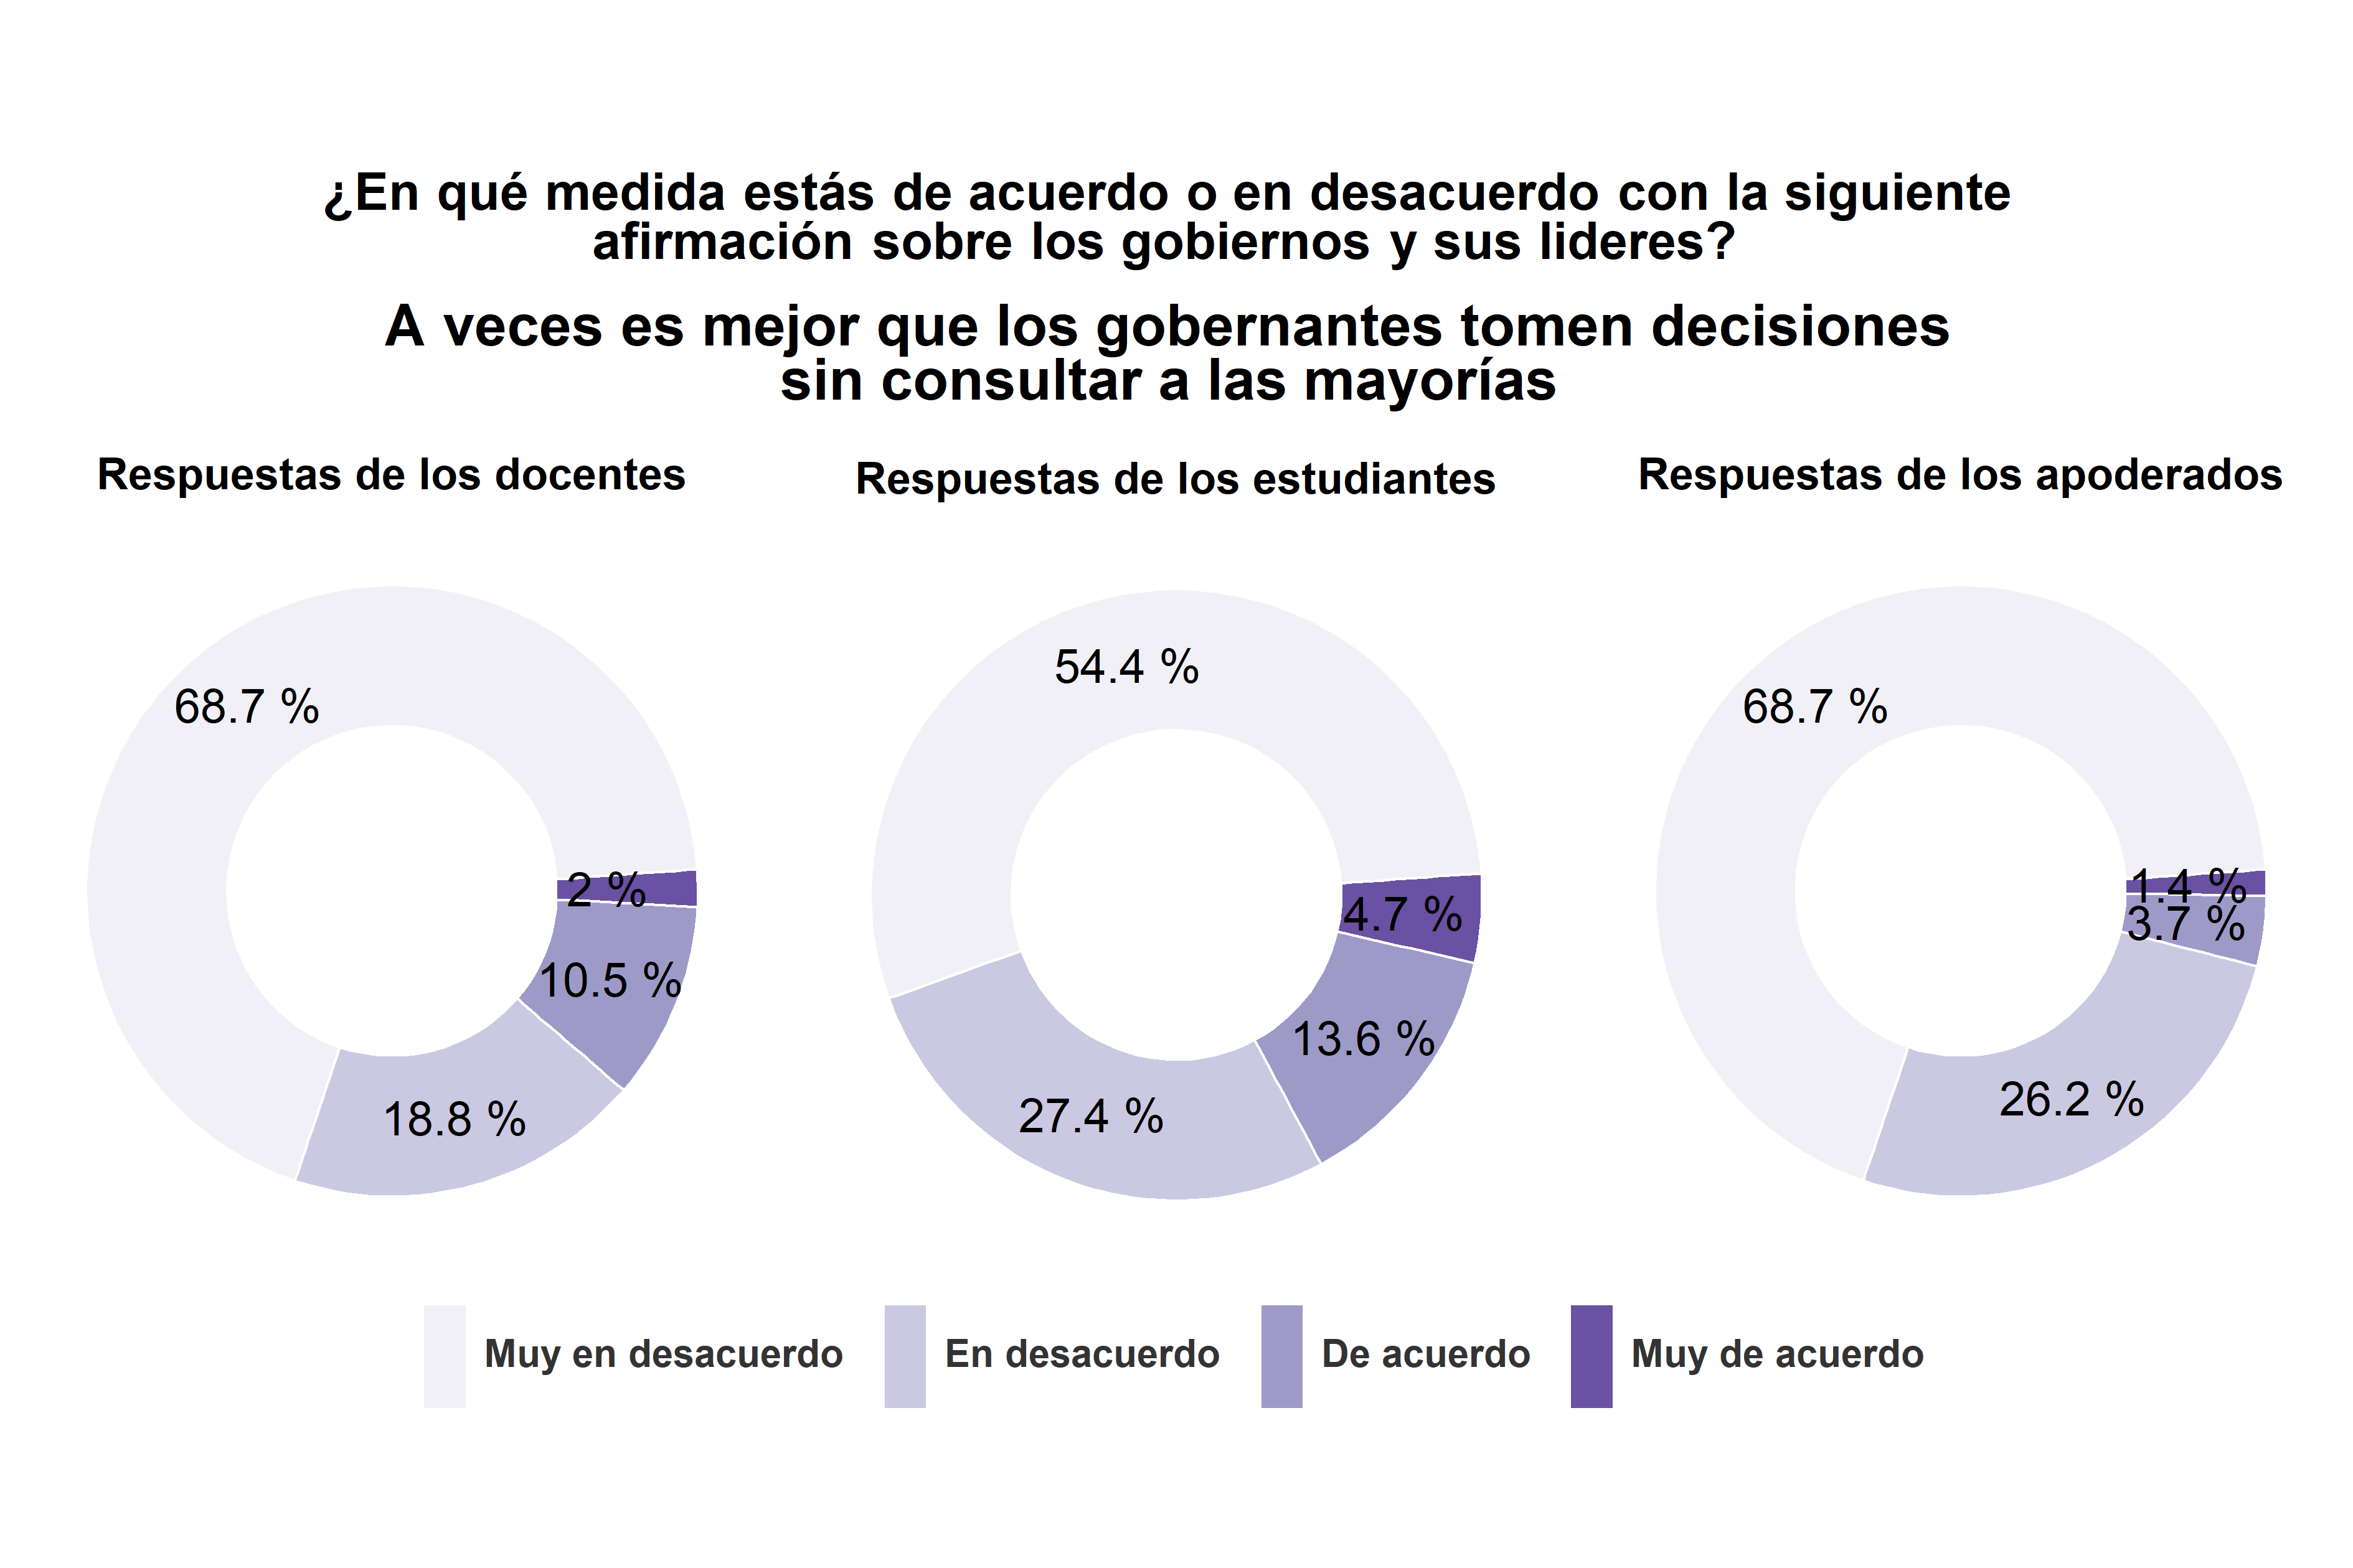
\includegraphics[width=0.8\linewidth,]{images/graph_aut4} 

}

\caption{A veces es mejor que se tomen decisiones sin consultar a las mayorías}\label{fig:unnamed-chunk-45}
\end{figure}

La mayoría de los docentes, estudiantes y apoderados está muy en desacuerdo con que \emph{a veces es mejor que los gobernantes tomen decisiones sin consultar a las mayorías} (un 68.7\%, un 54.4\% y un 68.7\%, respectivamente). La mayor parte de las personas restantes se encuentra en desacuerdo con la afirmación (un 18.8\% de los profesores, un 27.4\% de los estudiantes y un 26.2\% de los apoderados).

\begin{center}\rule{0.5\linewidth}{0.5pt}\end{center}

\begin{figure}[!ht]

{\centering 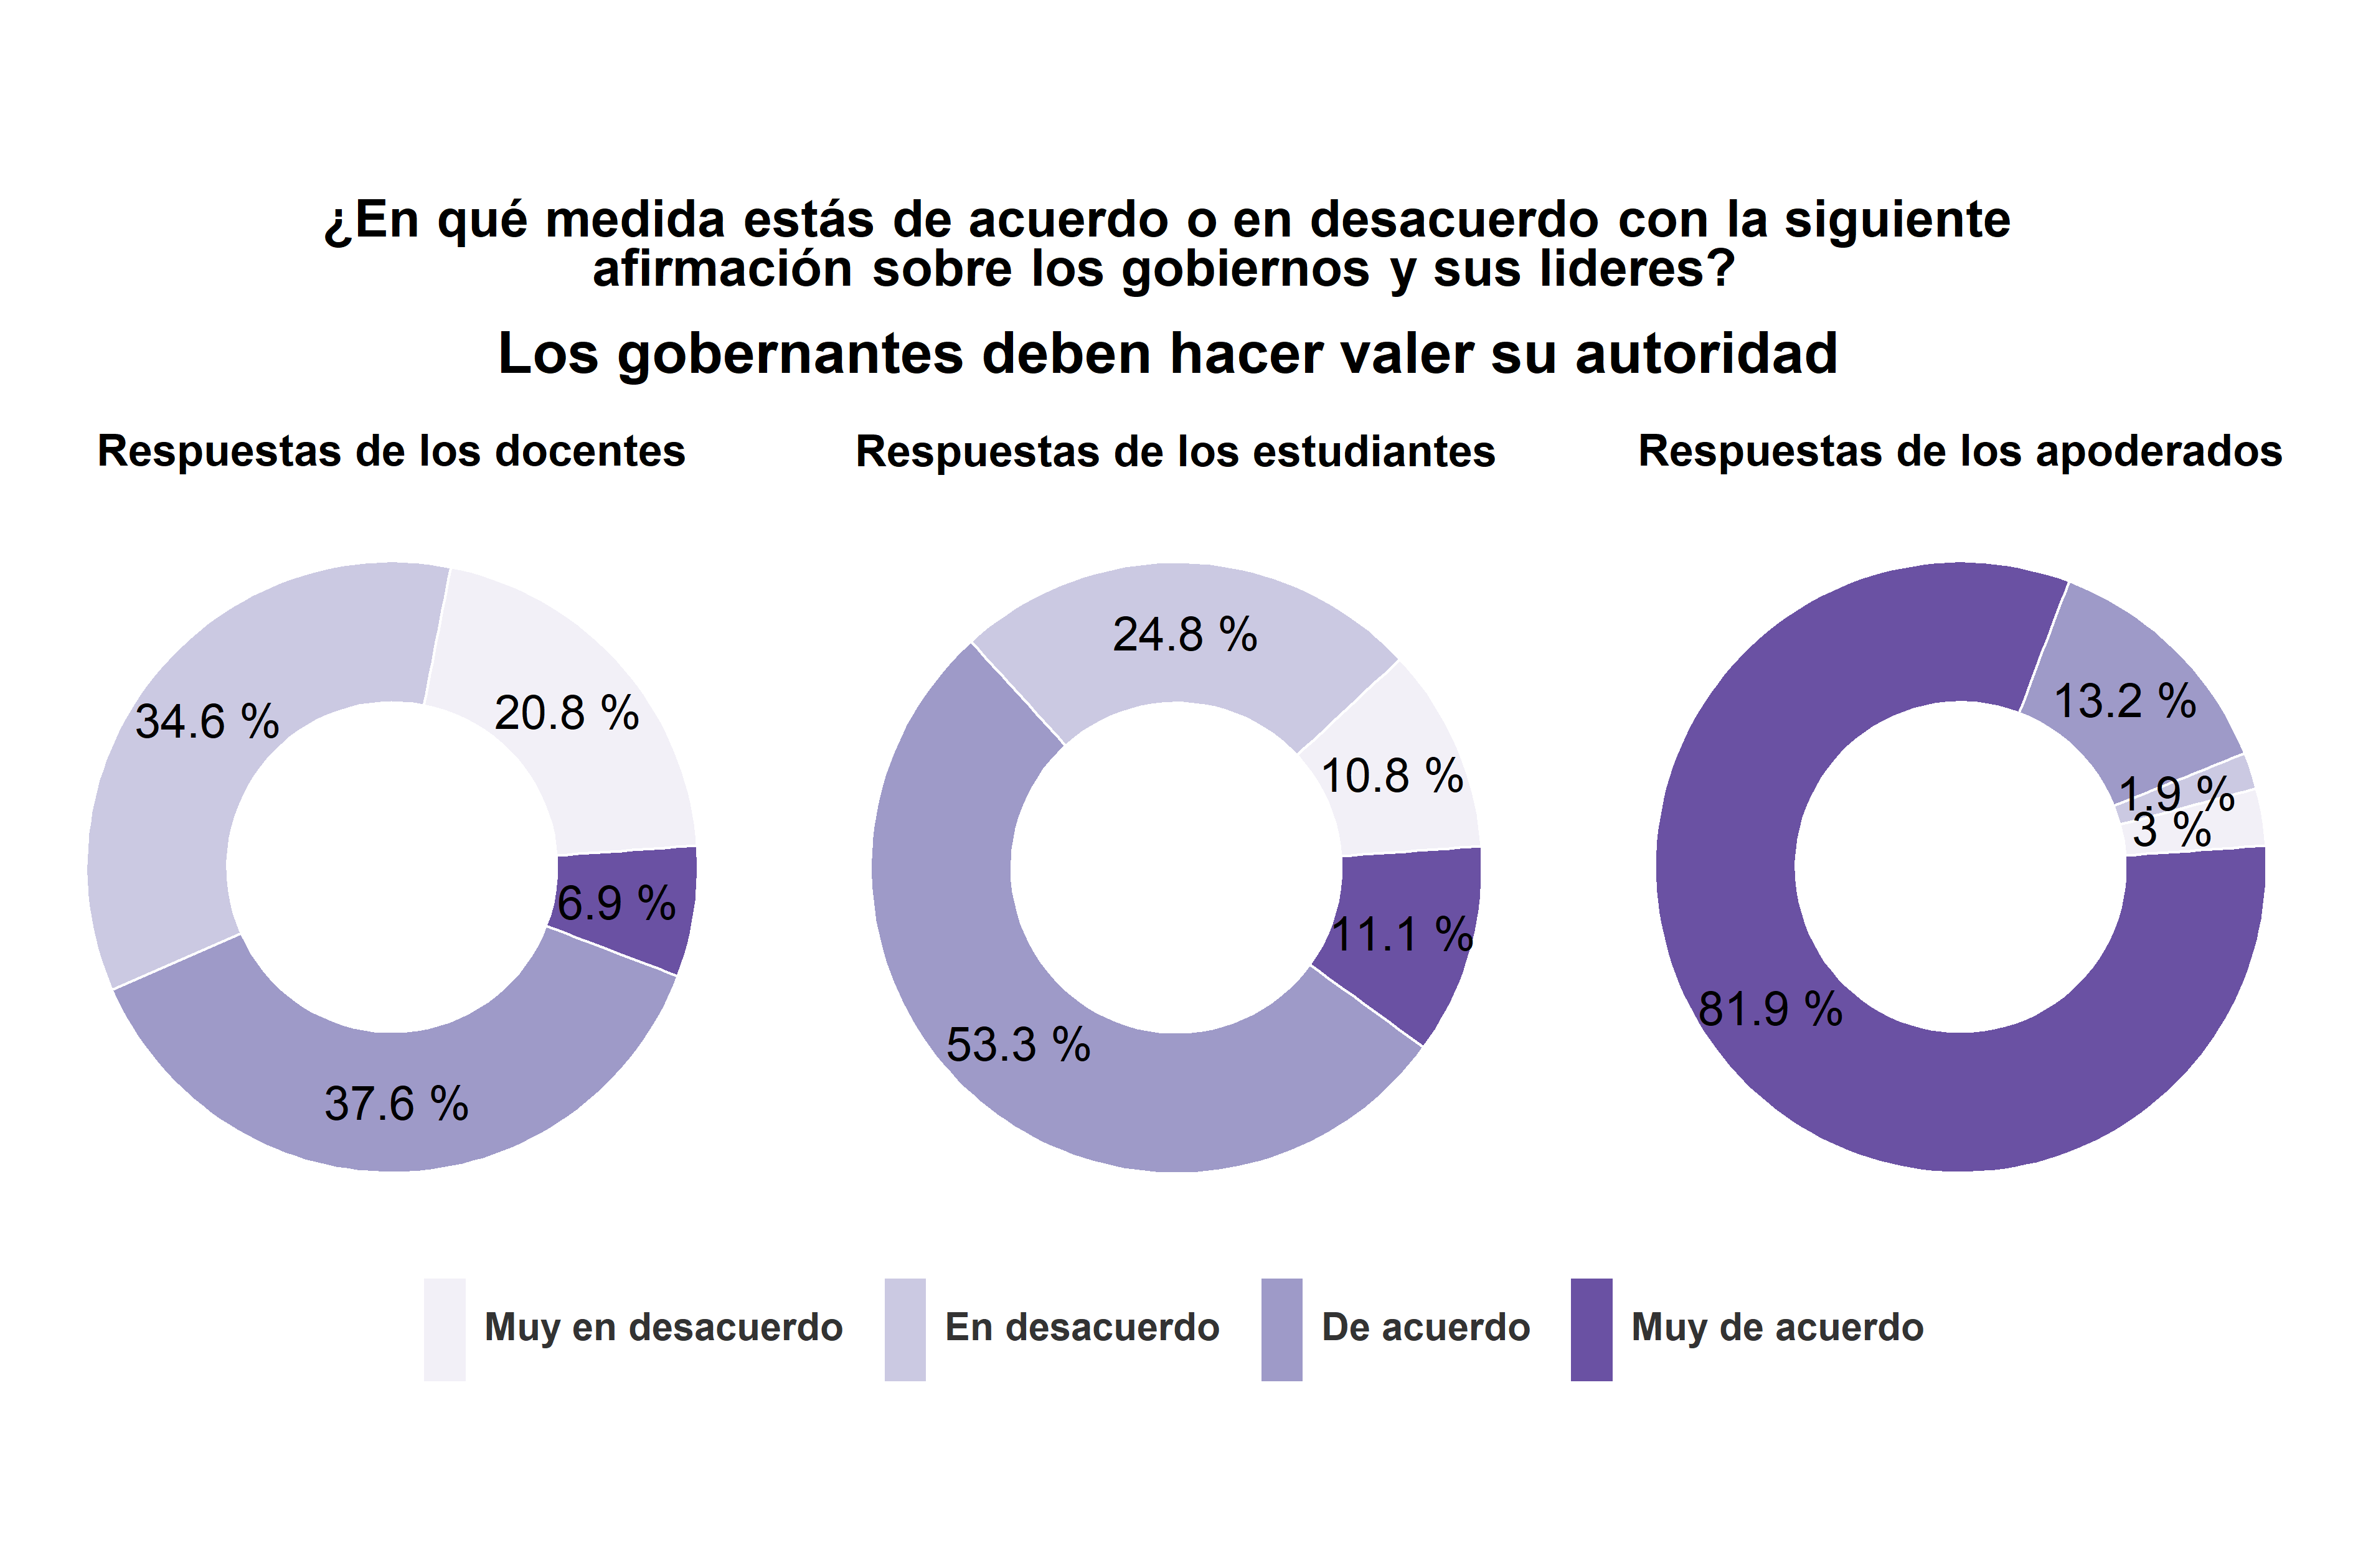
\includegraphics[width=0.8\linewidth,]{images/graph_aut5} 

}

\caption{Los gobernantes deben hacer valer su autoridad}\label{fig:unnamed-chunk-46}
\end{figure}

La mayoría de los apoderados está muy de acuerdo con que \emph{los gobernantes deben hacer valer su autoridad} (un 83.1\%) y la mayoría de los estudiantes se encuentra de acuerdo con la afirmación (un 52.5\%). Las respuestas de los docentes son más heterogéneas. Un 24.6\% de los docentes está muy en desacuerdo con la afirmación, un 26.2\% está en desacuerdo y un 41\% está de acuerdo.

\begin{center}\rule{0.5\linewidth}{0.5pt}\end{center}

\begin{figure}[!ht]

{\centering 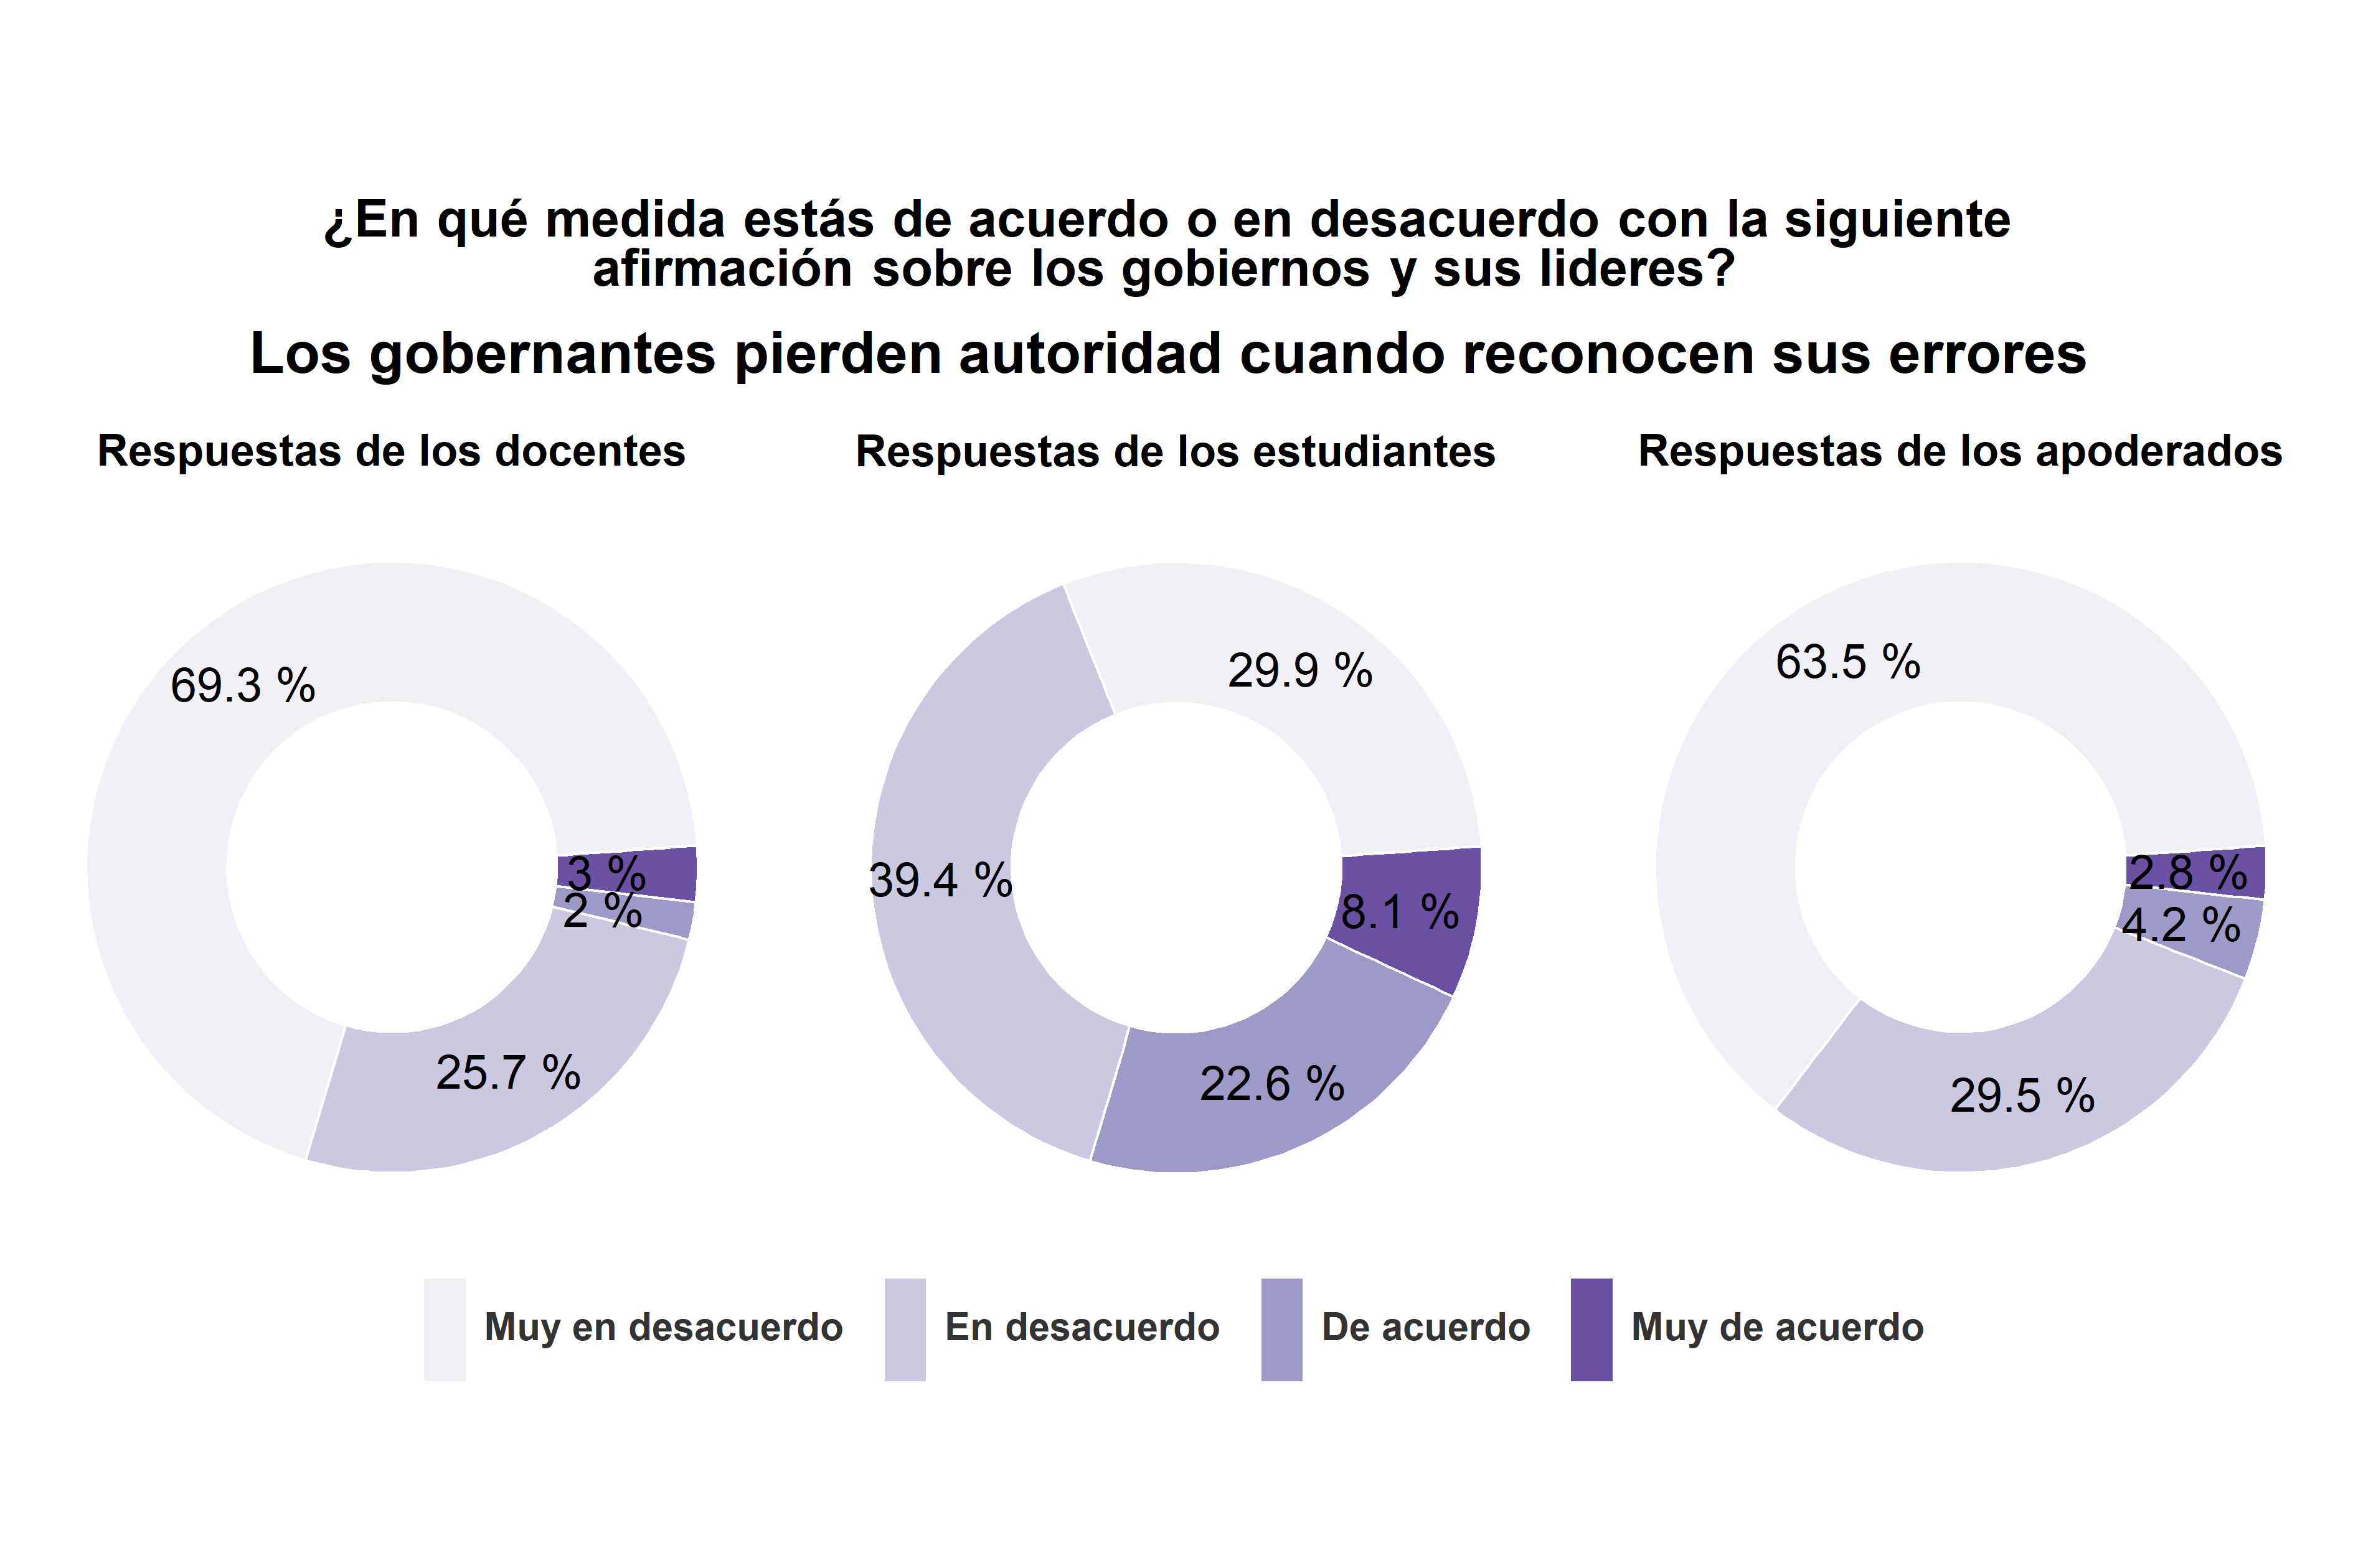
\includegraphics[width=0.8\linewidth,]{images/graph_aut6} 

}

\caption{Los gobernantes pierden autoridad cuando reconocen sus errores}\label{fig:unnamed-chunk-47}
\end{figure}

La mayoría de los docentes y apoderados está muy en desacuerdo con que \emph{los gobernantes pierden autoridad cuando reconocen sus errores} (un 72.1\% y un 66.1\%, respectivamente). La mayor parte de los estudiantes se encuentra muy en desacuerdo (un 33.1\%) o en desacuerdo con la afirmación (un 39.4\%).

\begin{center}\rule{0.5\linewidth}{0.5pt}\end{center}

\begin{figure}[!ht]

{\centering 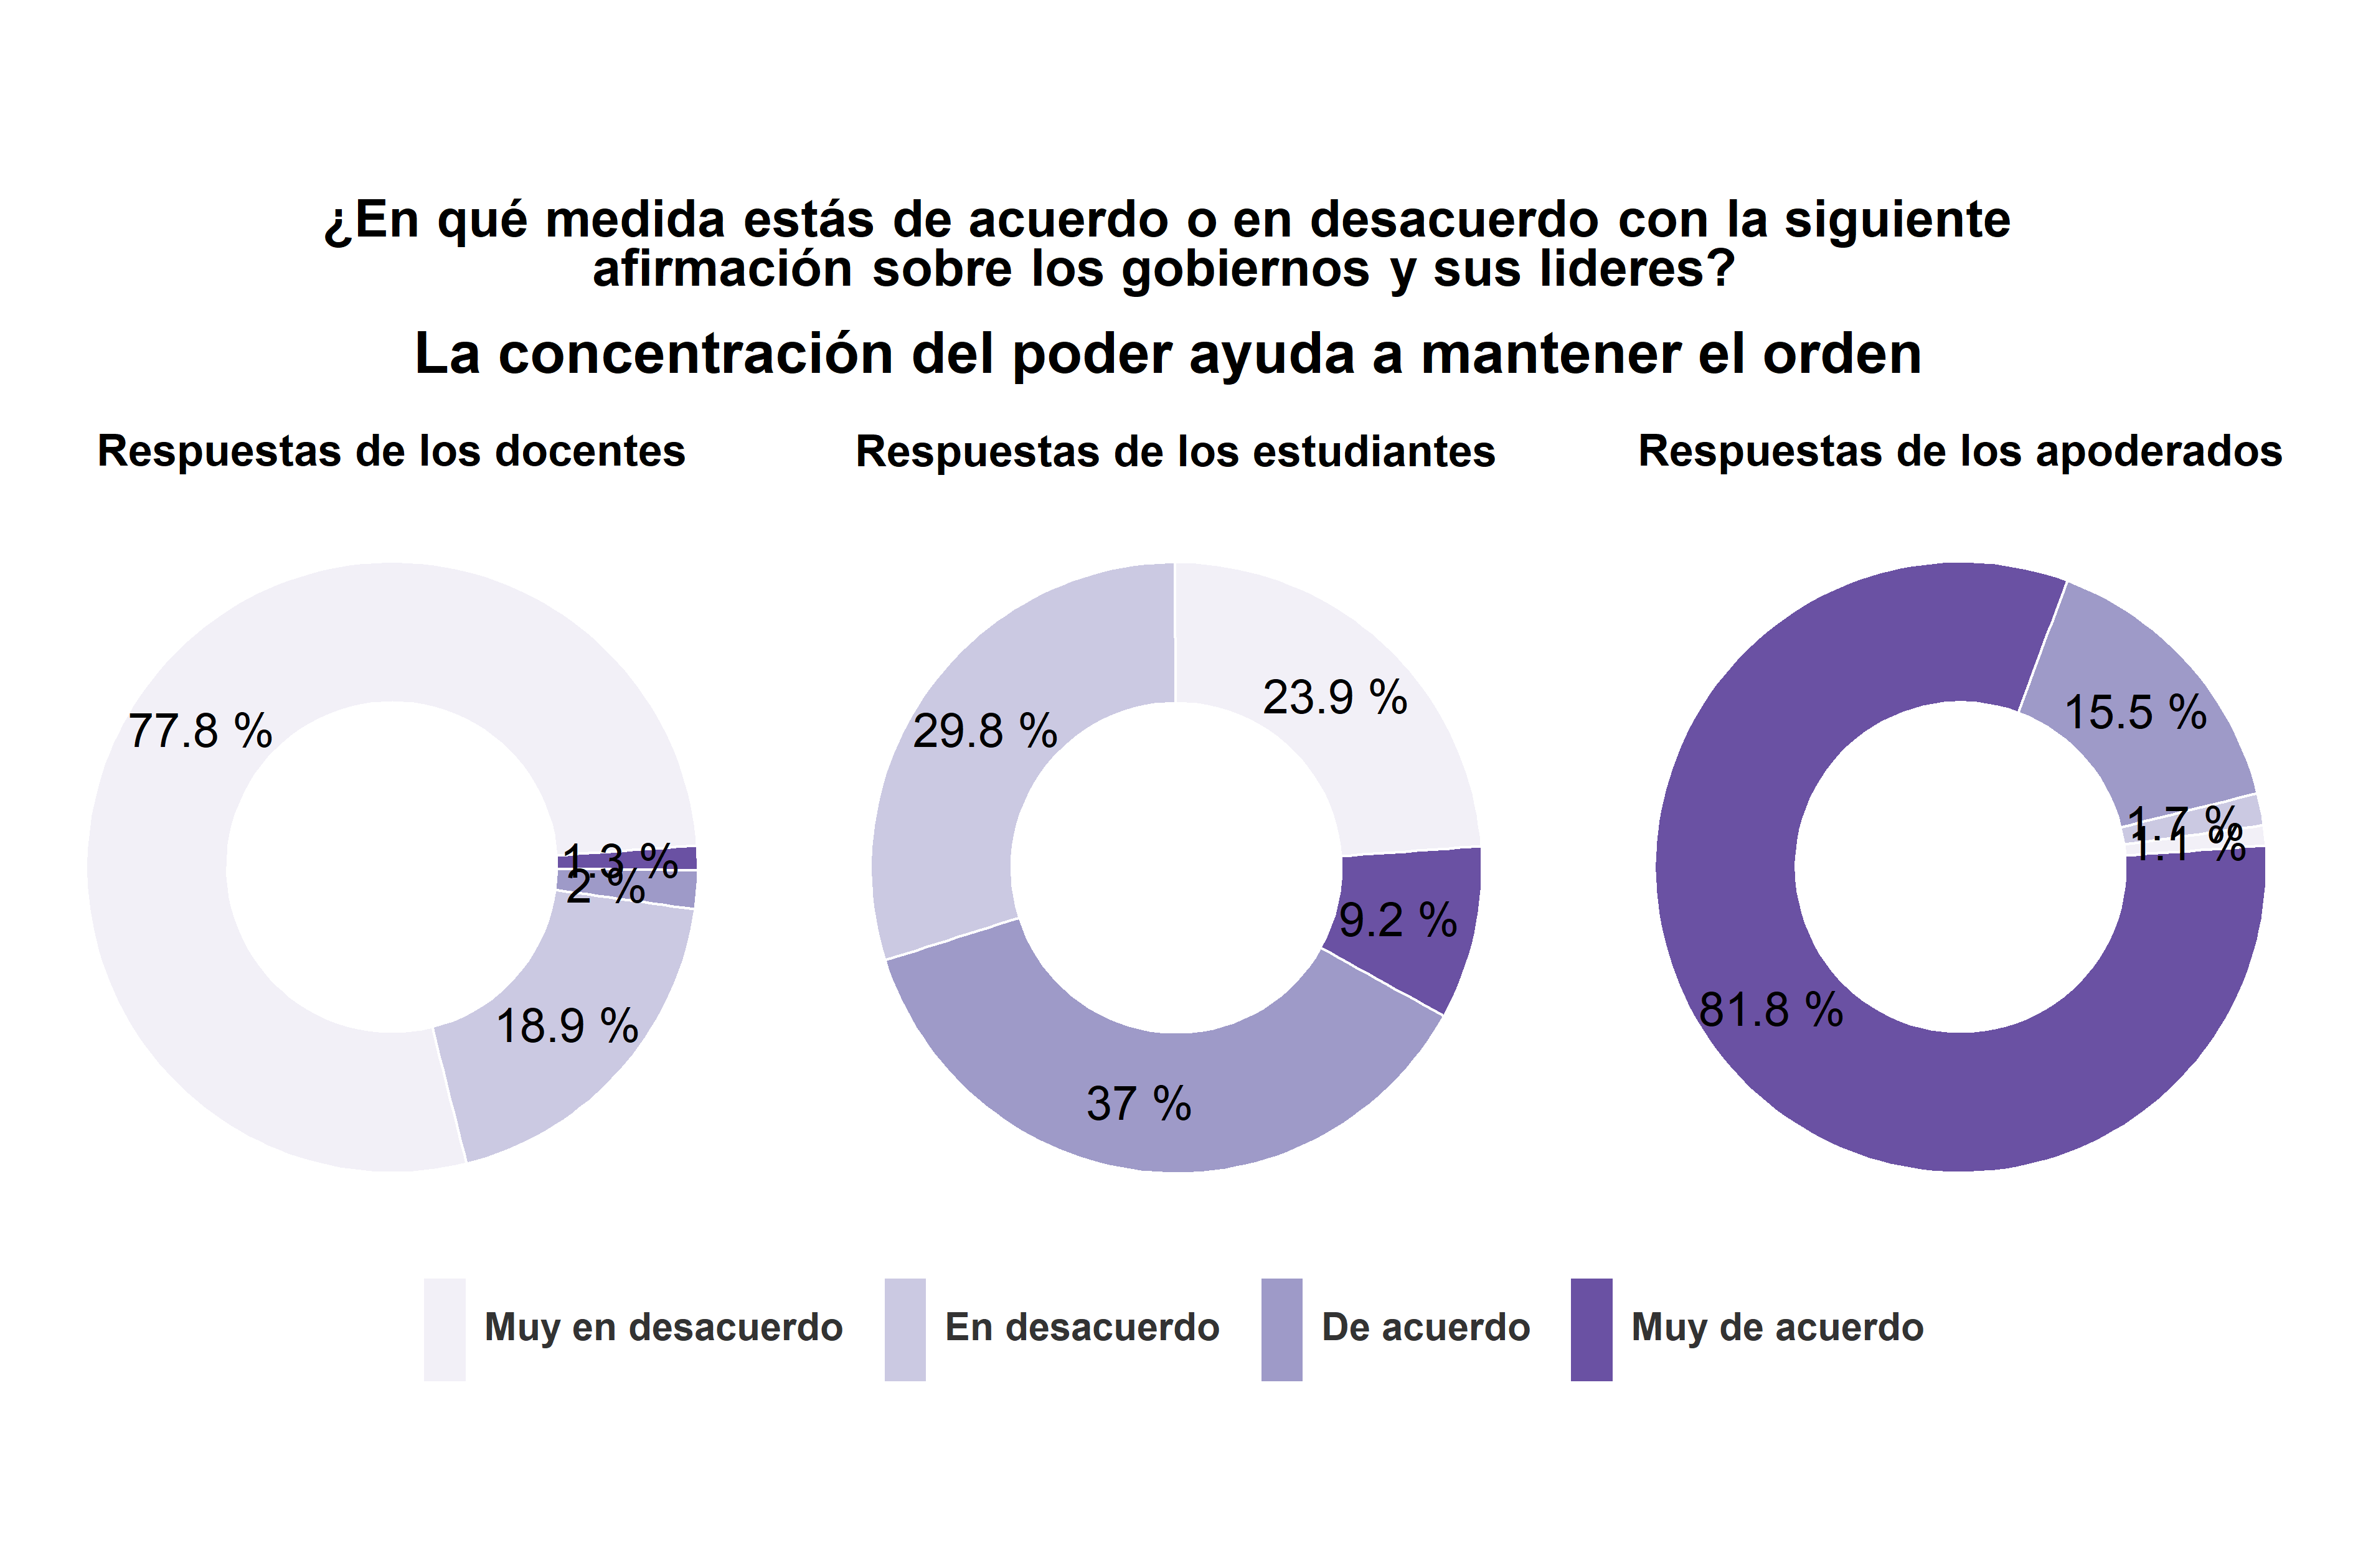
\includegraphics[width=0.8\linewidth,]{images/graph_aut7} 

}

\caption{Concentrar el poder ayuda a mantener el orden}\label{fig:unnamed-chunk-48}
\end{figure}

La mayoría de los docentes está muy en desacuerdo con que \emph{la concentración del poder ayuda a mantener el orden} (un 77.8\%) y, por el contrario, la mayoría de los apoderados se encuentra muy de acuerdo con esta afirmación (un 81.8\%). La opinión de los estudiantes es más diversa. Un 29.8\% de los estudiantes está en desacuerdo con la afirmación y un 37\% está de acuerdo.

\begin{center}\rule{0.5\linewidth}{0.5pt}\end{center}

\begin{figure}[!ht]

{\centering 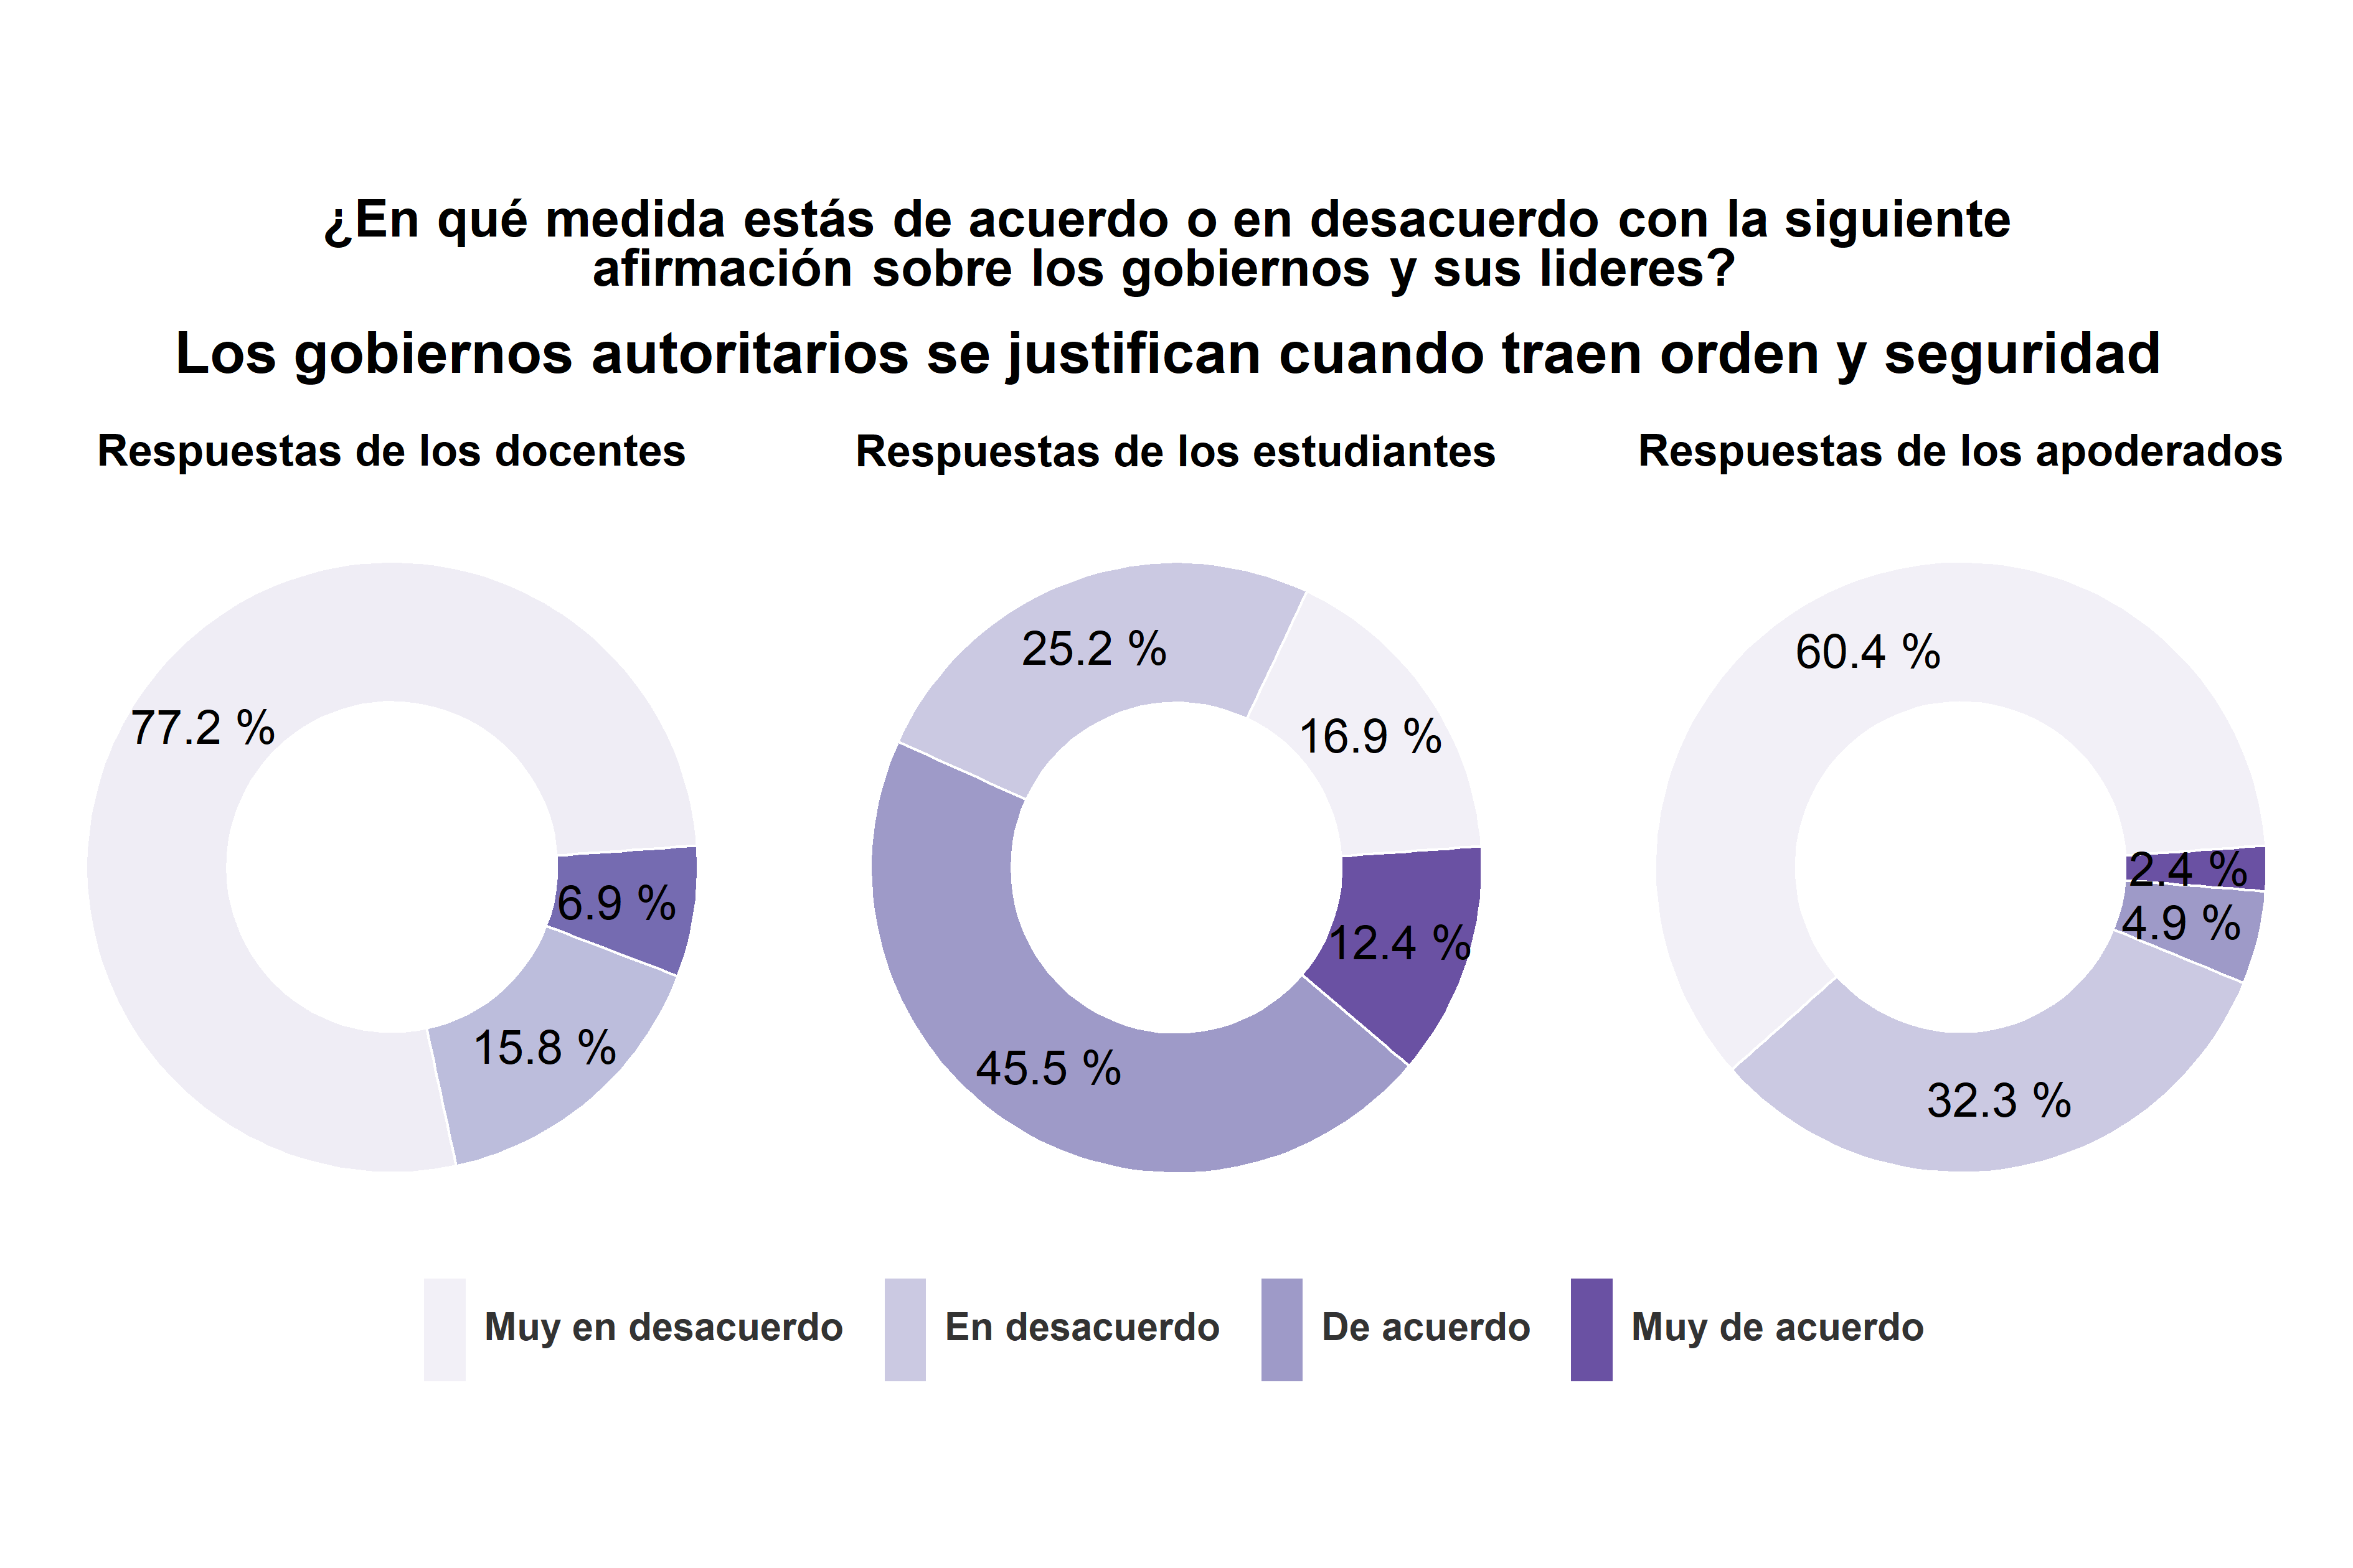
\includegraphics[width=0.8\linewidth,]{images/graph_aut8} 

}

\caption{El orden y la seguridad justifican los gobiernos autoritarios}\label{fig:unnamed-chunk-49}
\end{figure}

La mayoría de los docentes y apoderados está muy en desacuerdo con que \emph{los gobiernos autoritarios se justifican cuando traen orden y seguridad} (un 80.5\% y un 62.4\%, respectivamente). Mientras que la mayor parte de los estudiantes se encuentra de acuerdo con la afirmación (un 44.1\%).

\begin{center}\rule{0.5\linewidth}{0.5pt}\end{center}

\begin{figure}[!ht]

{\centering 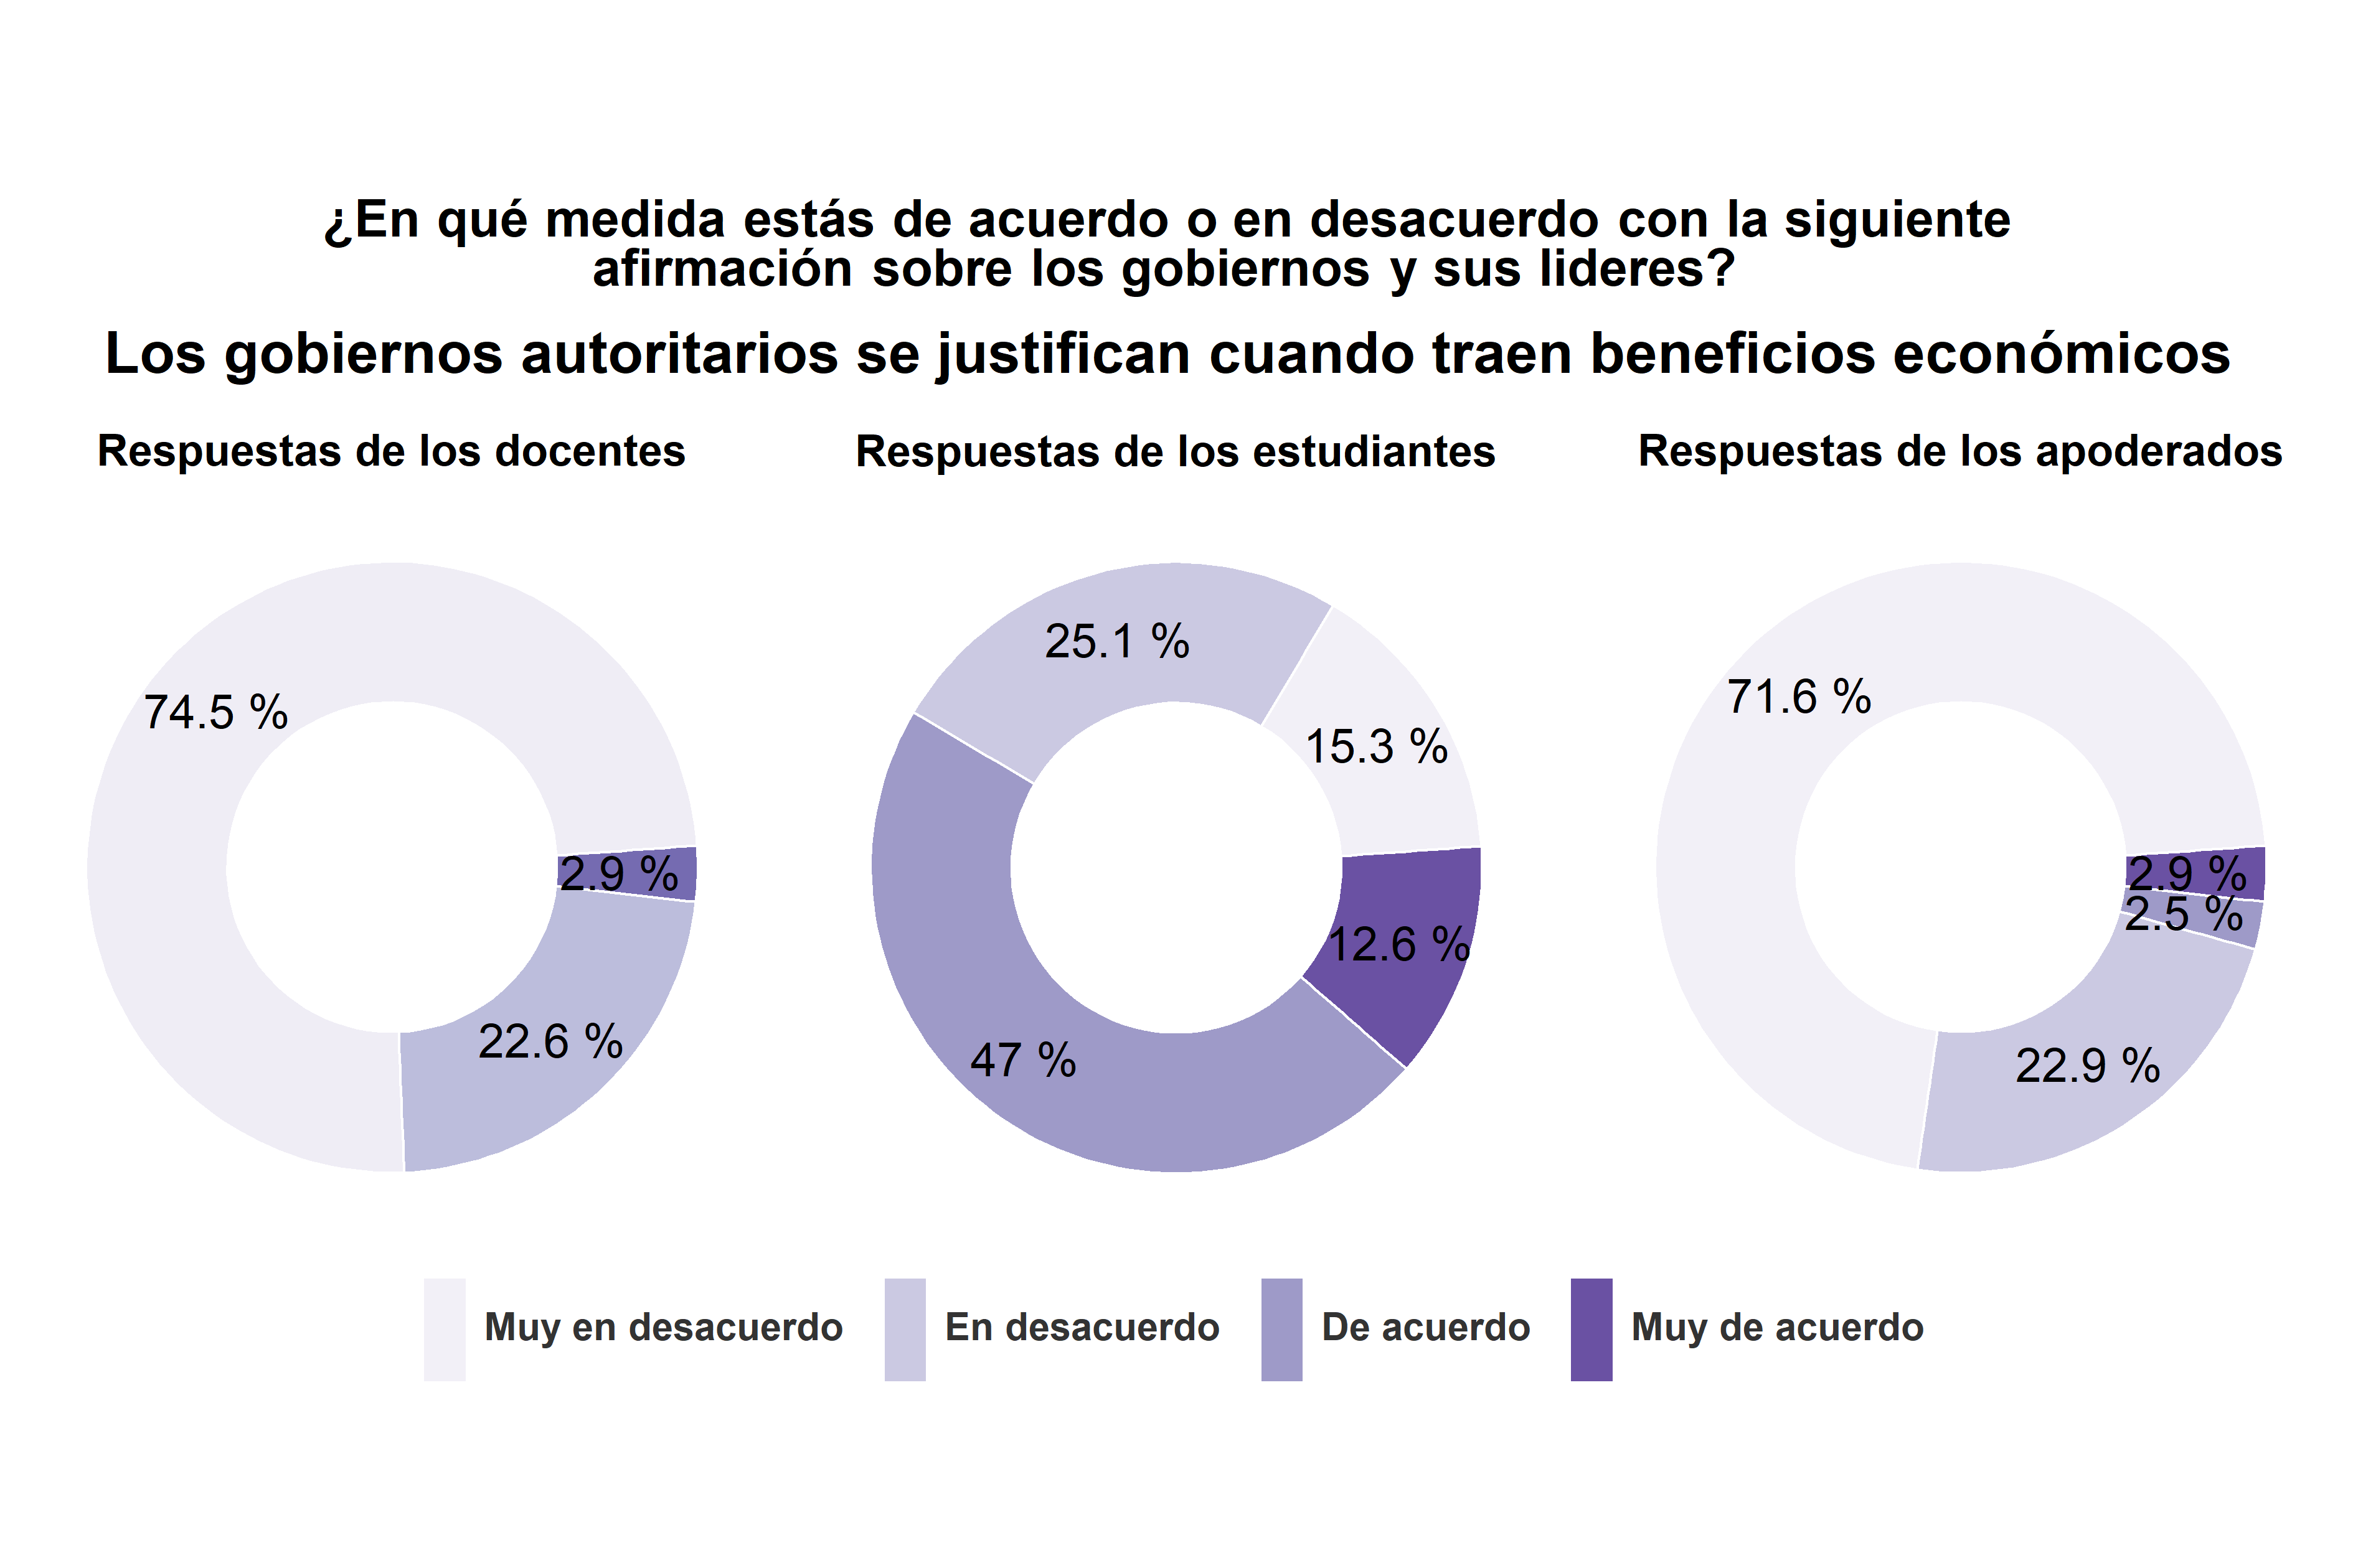
\includegraphics[width=0.8\linewidth,]{images/graph_aut9} 

}

\caption{Los beneficios económicos justifican los gobiernos autoritarios}\label{fig:unnamed-chunk-50}
\end{figure}

La mayoría de los docentes y apoderados está muy en desacuerdo con que \emph{los gobiernos autoritarios se justifican cuando traen beneficios económicos} (un 76.1\% y un 75.4\%, respectivamente). Por el contrario, la mayor parte de los estudiantes se encuentra de acuerdo con la afirmación (un 45\%).

\begin{center}\rule{0.5\linewidth}{0.5pt}\end{center}

\hypertarget{confianza-en-instituciones}{%
\section{Confianza en instituciones}\label{confianza-en-instituciones}}

\begin{center}\rule{0.5\linewidth}{0.5pt}\end{center}

\begin{figure}[!ht]

{\centering 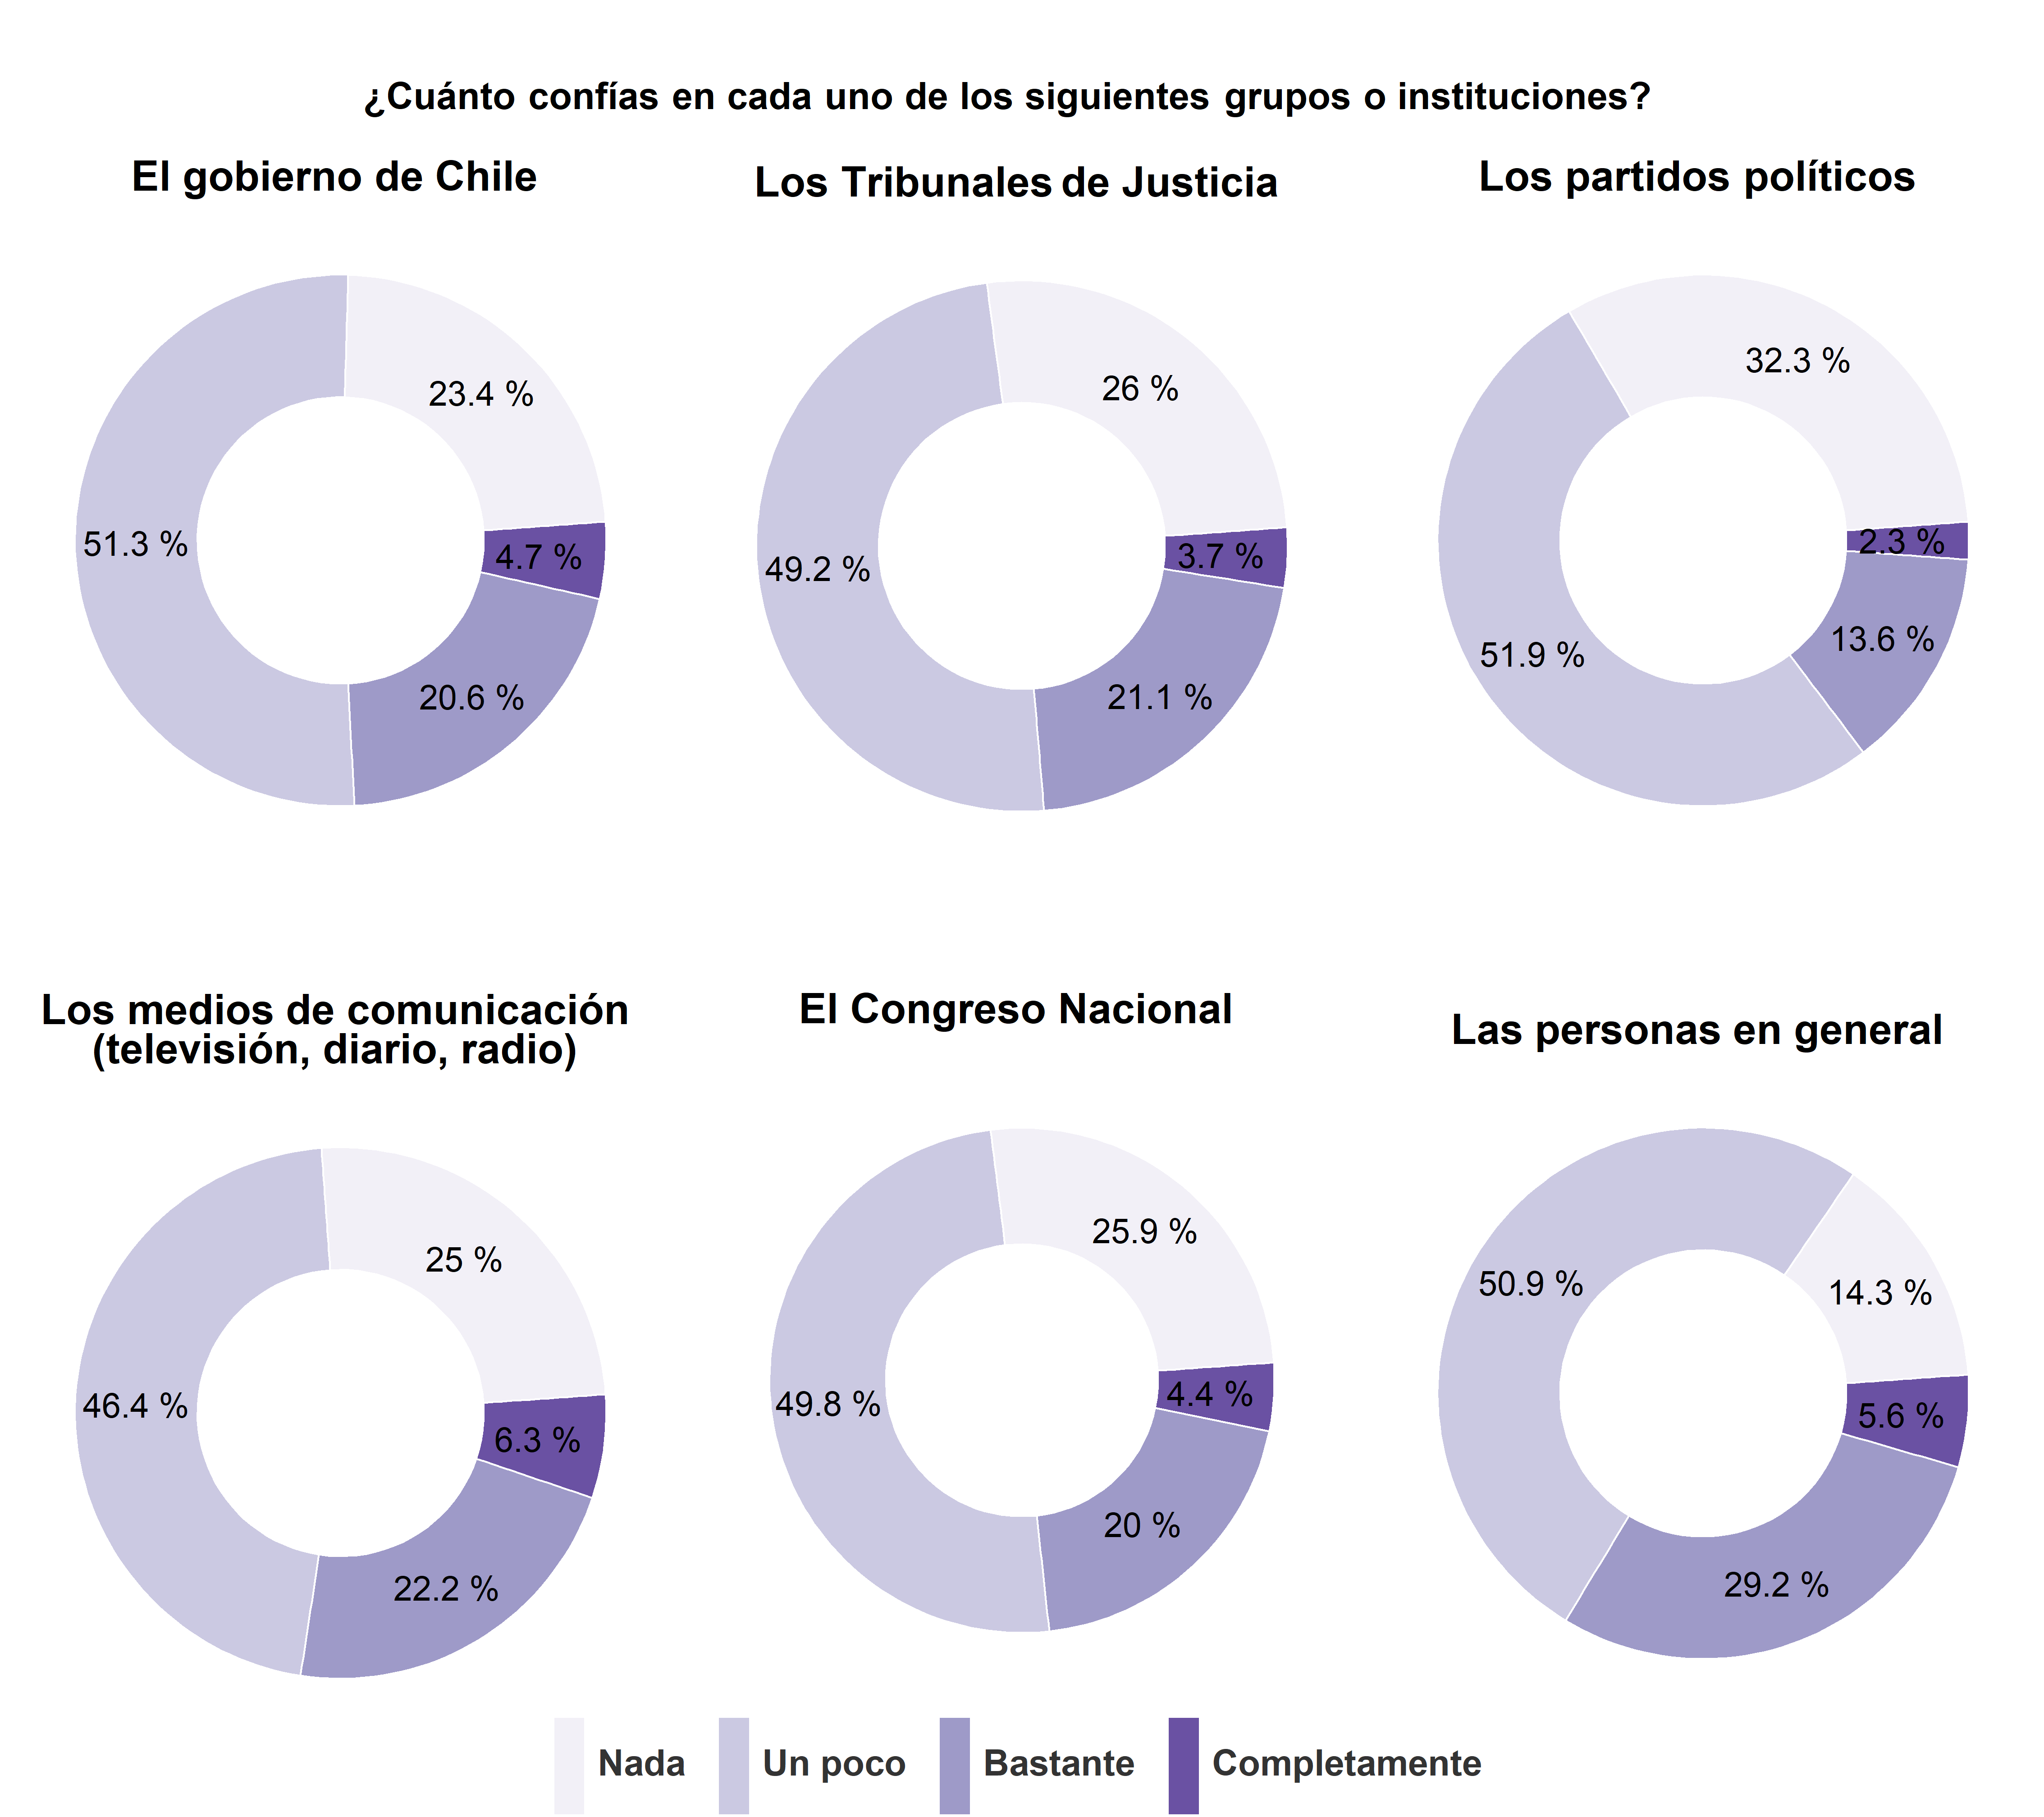
\includegraphics[width=0.8\linewidth,]{images/graph_cgp} 

}

\caption{Confianza en grupos e instituciones}\label{fig:unnamed-chunk-51}
\end{figure}

La mayoría de los estudiantes confía nada o un poco en los grupos e instituciones por los que se consultó. La institución en la que menos confían los estudiantes corresponde a \emph{los partidos políticos}. El 35\% de los estudiantes declaro que confía nada en los partidos políticos y el 52.1\% señaló que confía un poco en esta institución. El grupo en el que más confían los estudiantes corresponde a \emph{las personas en general}. El 28.9\% de los estudiantes confía bastante en las personas en general y el 4.3\% confía completamente en este grupo.

\begin{center}\rule{0.5\linewidth}{0.5pt}\end{center}

\hypertarget{participaciuxf3n}{%
\chapter{Participación}\label{participaciuxf3n}}

En este módulo se presentan las respuestas de los estudiantes a una serie de preguntas sobre su participación en distintas actividades al interior de la escuela y fuera de la escuela. El reporte de los resultados se organiza en tres secciones. En la primera sección se presentarán los resultados de preguntas sobre la participación formal de los estudiantes en actividades al interior de la escuela y sobre la disposición de los estudiantes a participar en instancias políticas formales cuando sea adulto. En la segunda sección se expondrán los resultados a preguntas sobre la participación activista de los estudiantes en actividades al interior de la escuela y fuera de esta. En la tercera sección se mostrarán los resultados de preuntas sobre la participación comunitaria de los estudiantes en actividades al interior de la escuela y fuera de esta.

En términos generales, cabe destacar que la participación de los estudiantes se concentra en actividades realizadas al interior de la escuela. Las actividades que han sido realizadas por una mayor proporción de estudiantes son: votar en una elección, firmar una petición, trabajos voluntarios de ayuda, colectas de dineros o bienes para ayudar a otros y actividades de ayuda a la comunidad.

\hypertarget{participaciuxf3n-formal}{%
\section{Participación formal}\label{participaciuxf3n-formal}}

\begin{center}\rule{0.5\linewidth}{0.5pt}\end{center}

\begin{figure}[!ht]

{\centering 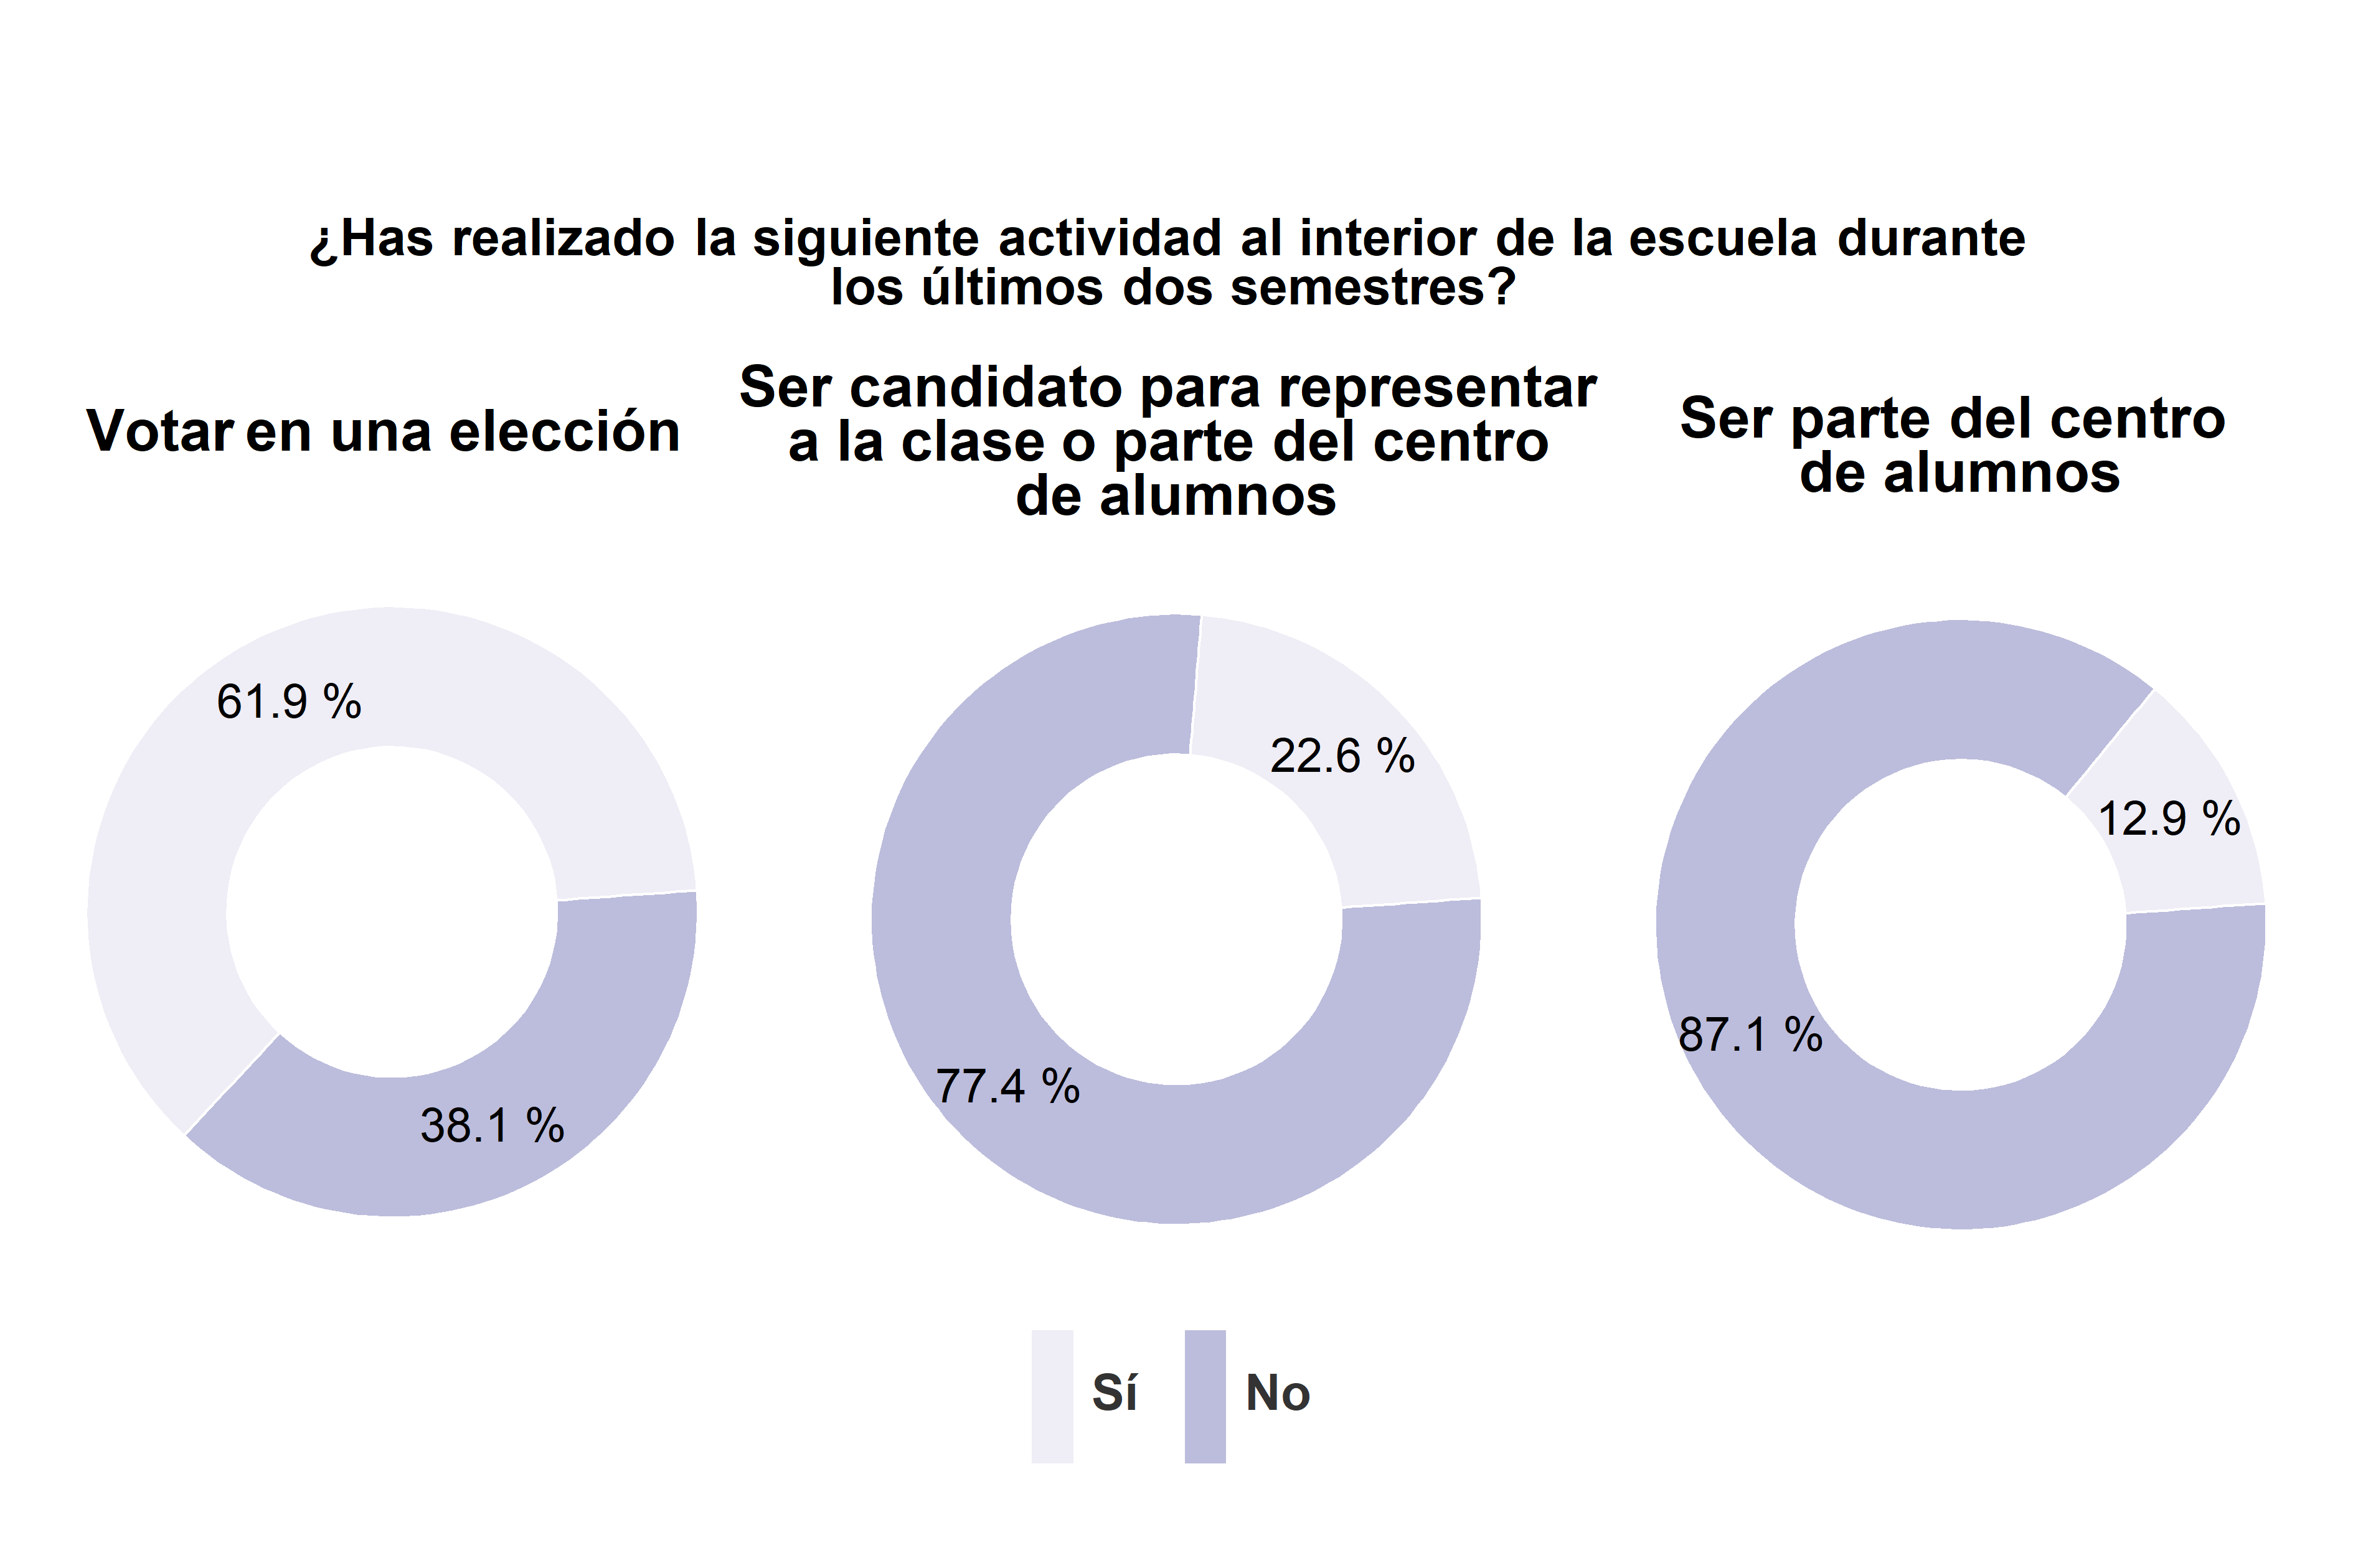
\includegraphics[width=0.8\linewidth,]{images/graph_partform_act} 

}

\caption{Participación formal al interior de la escuela}\label{fig:unnamed-chunk-52}
\end{figure}

En relación con la participación en votaciones, la mayoría de los estudiantes declara que ha votado en una elección al interior de su escuela durante los últimos dos semestres (un 61.9\%). En relación con la postulación a cargos de representación, la mayoría de los estudiantes señala que durante los últimos dos semestres no ha sido candidato para representar a la clase o para ser parte del centro de alumnos (un 77.4\%), ni tampoco ha sido efectivamente parte del centro de alumnos (un 87.1\%).

\begin{center}\rule{0.5\linewidth}{0.5pt}\end{center}

\begin{figure}[!ht]

{\centering 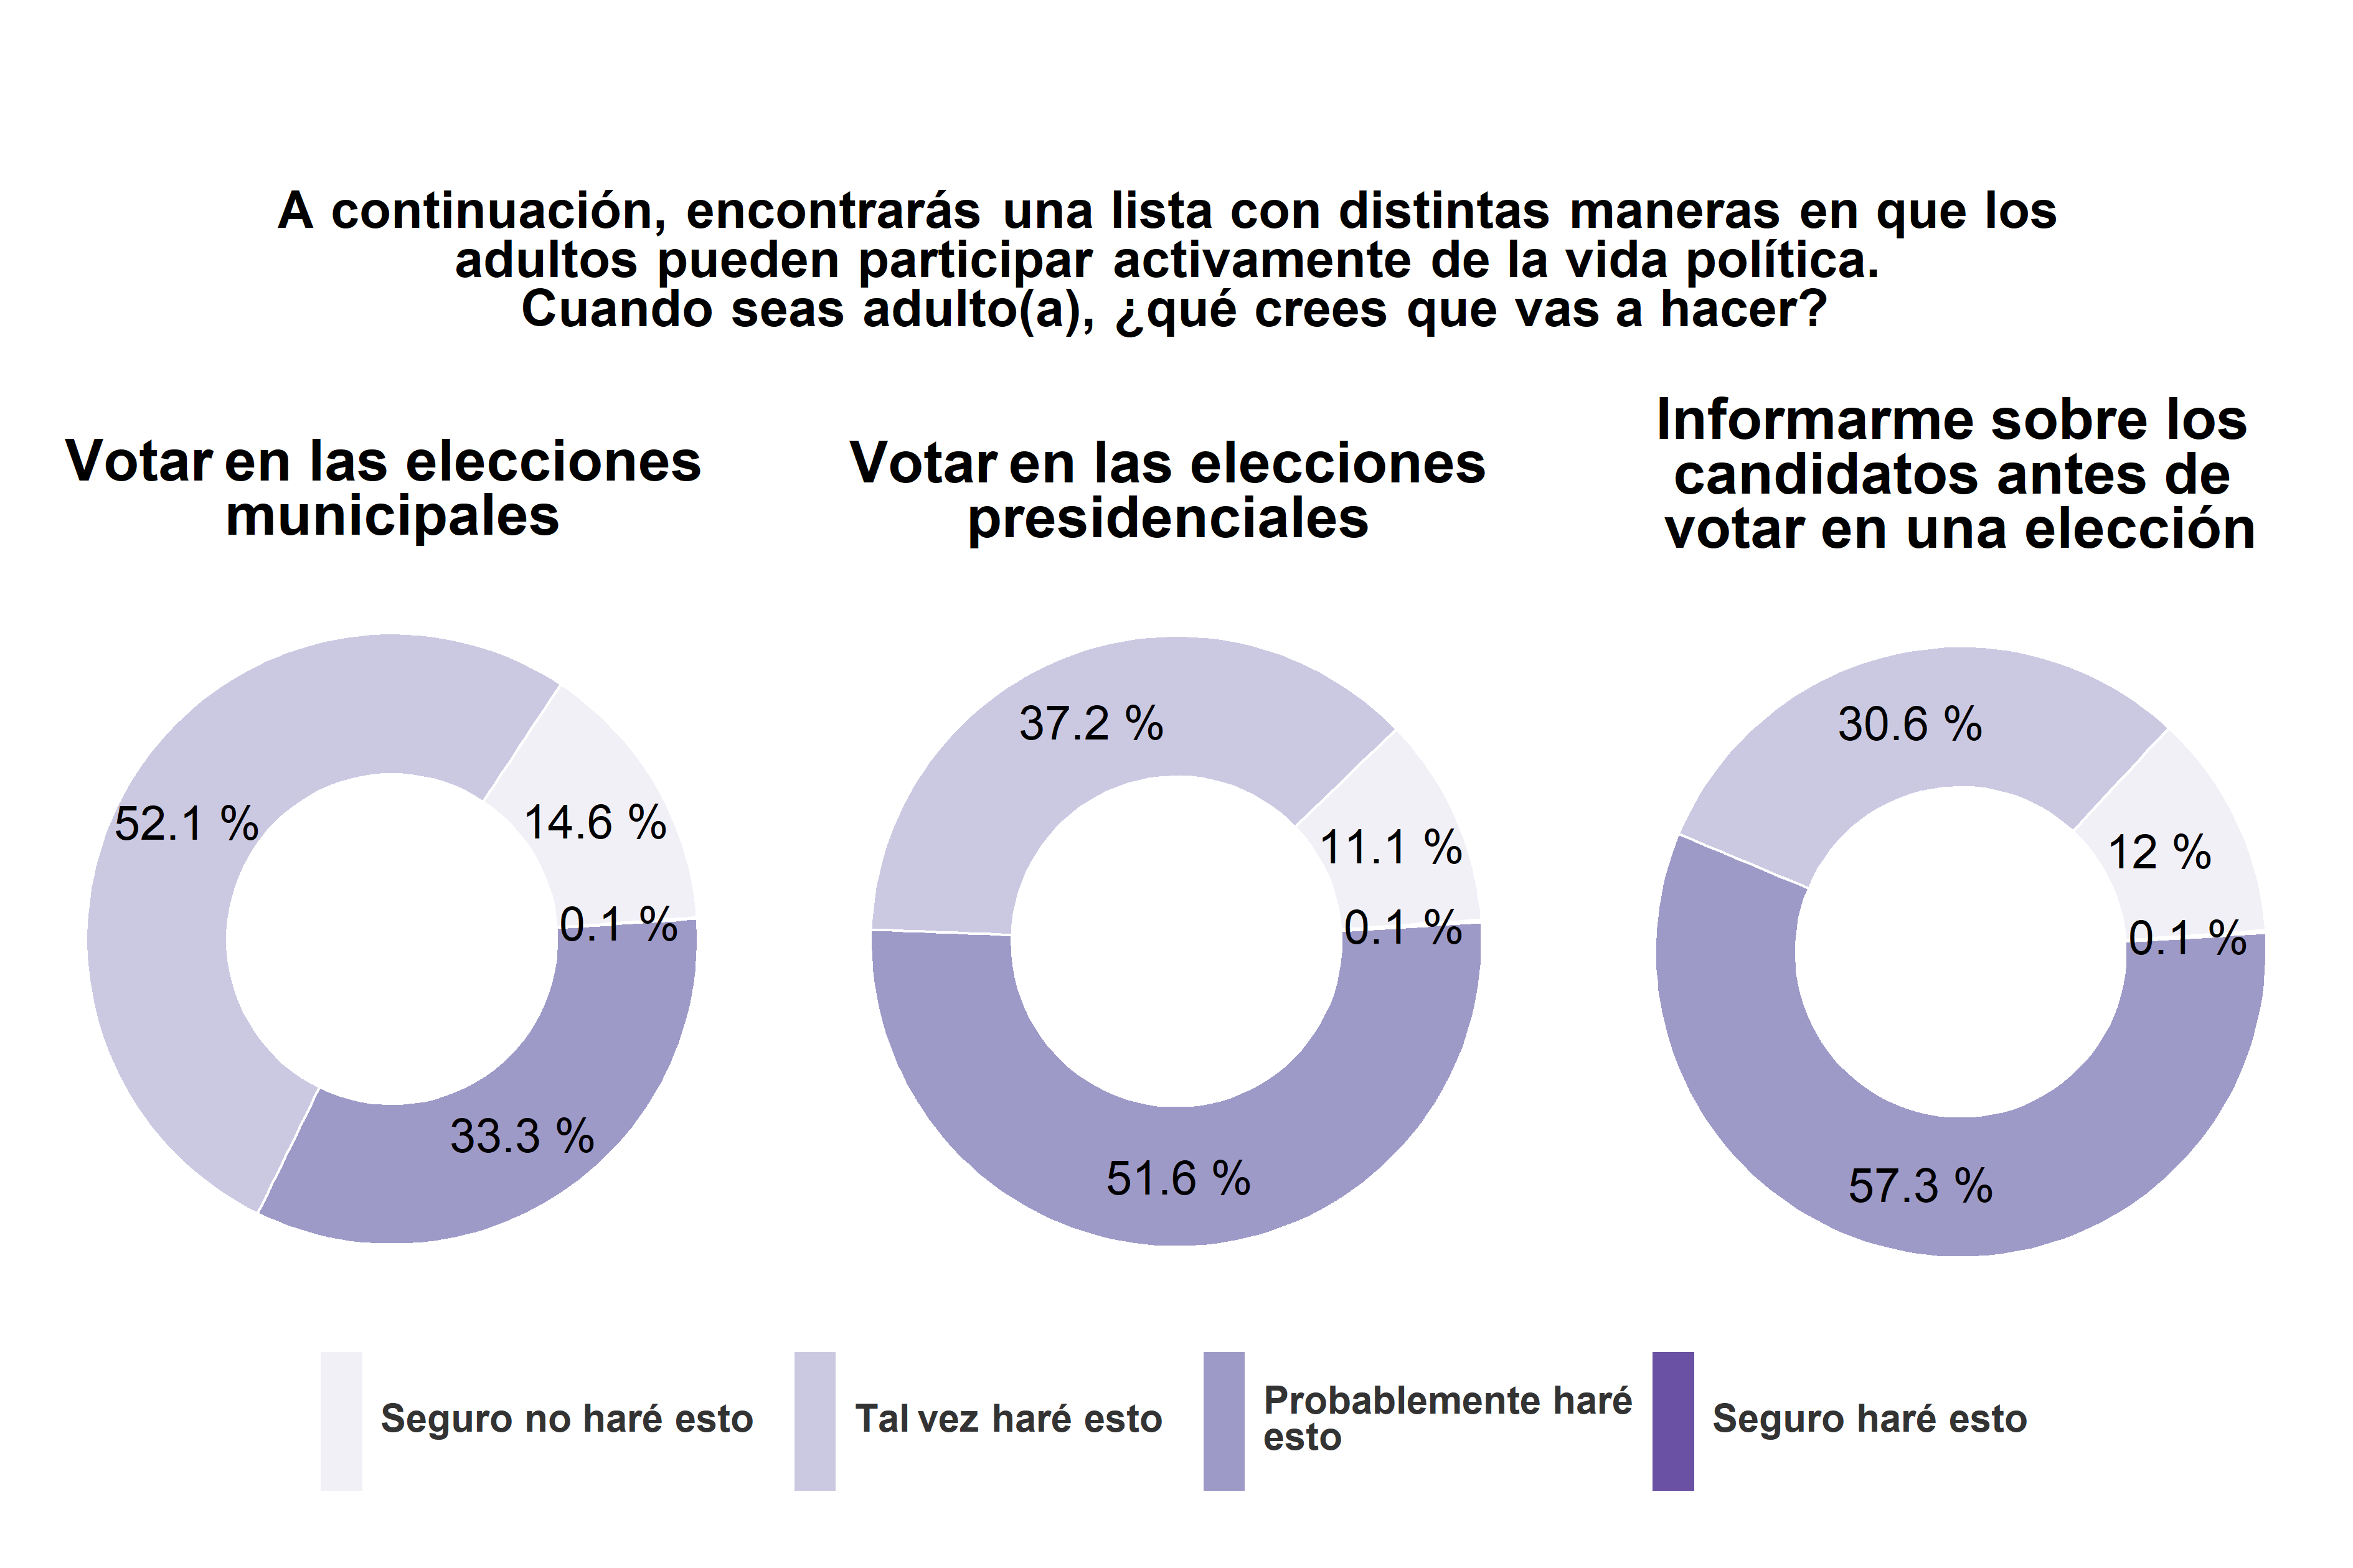
\includegraphics[width=0.8\linewidth,]{images/graph_partform_fut} 

}

\caption{Participación formal cuando sea adulto(a)}\label{fig:unnamed-chunk-53}
\end{figure}

Al consultar a los estudiantes sobre su disposición a participar activamente de la vida política cuando adulto, solo un 0.1\% responde ``seguro haré esto'' ante las distintas actividades que se les presentan. Respecto a votar en las elecciones municipales, la mayoría de los estudiantes señala que tal vez lo hará (un 50.7\%). En relación con las otras dos actividades, la mayoría de los estudiantes declara que probablemente lo hará. Más específicamente, el 56\% dice que probablemente votará en las elecciones presidenciales y el 60.9\% señala que probablemente se informará sobre los candidatos antes de votar en una elección.

\begin{center}\rule{0.5\linewidth}{0.5pt}\end{center}

\hypertarget{participaciuxf3n-activista}{%
\section{Participación activista}\label{participaciuxf3n-activista}}

\begin{center}\rule{0.5\linewidth}{0.5pt}\end{center}

\begin{figure}[!ht]

{\centering 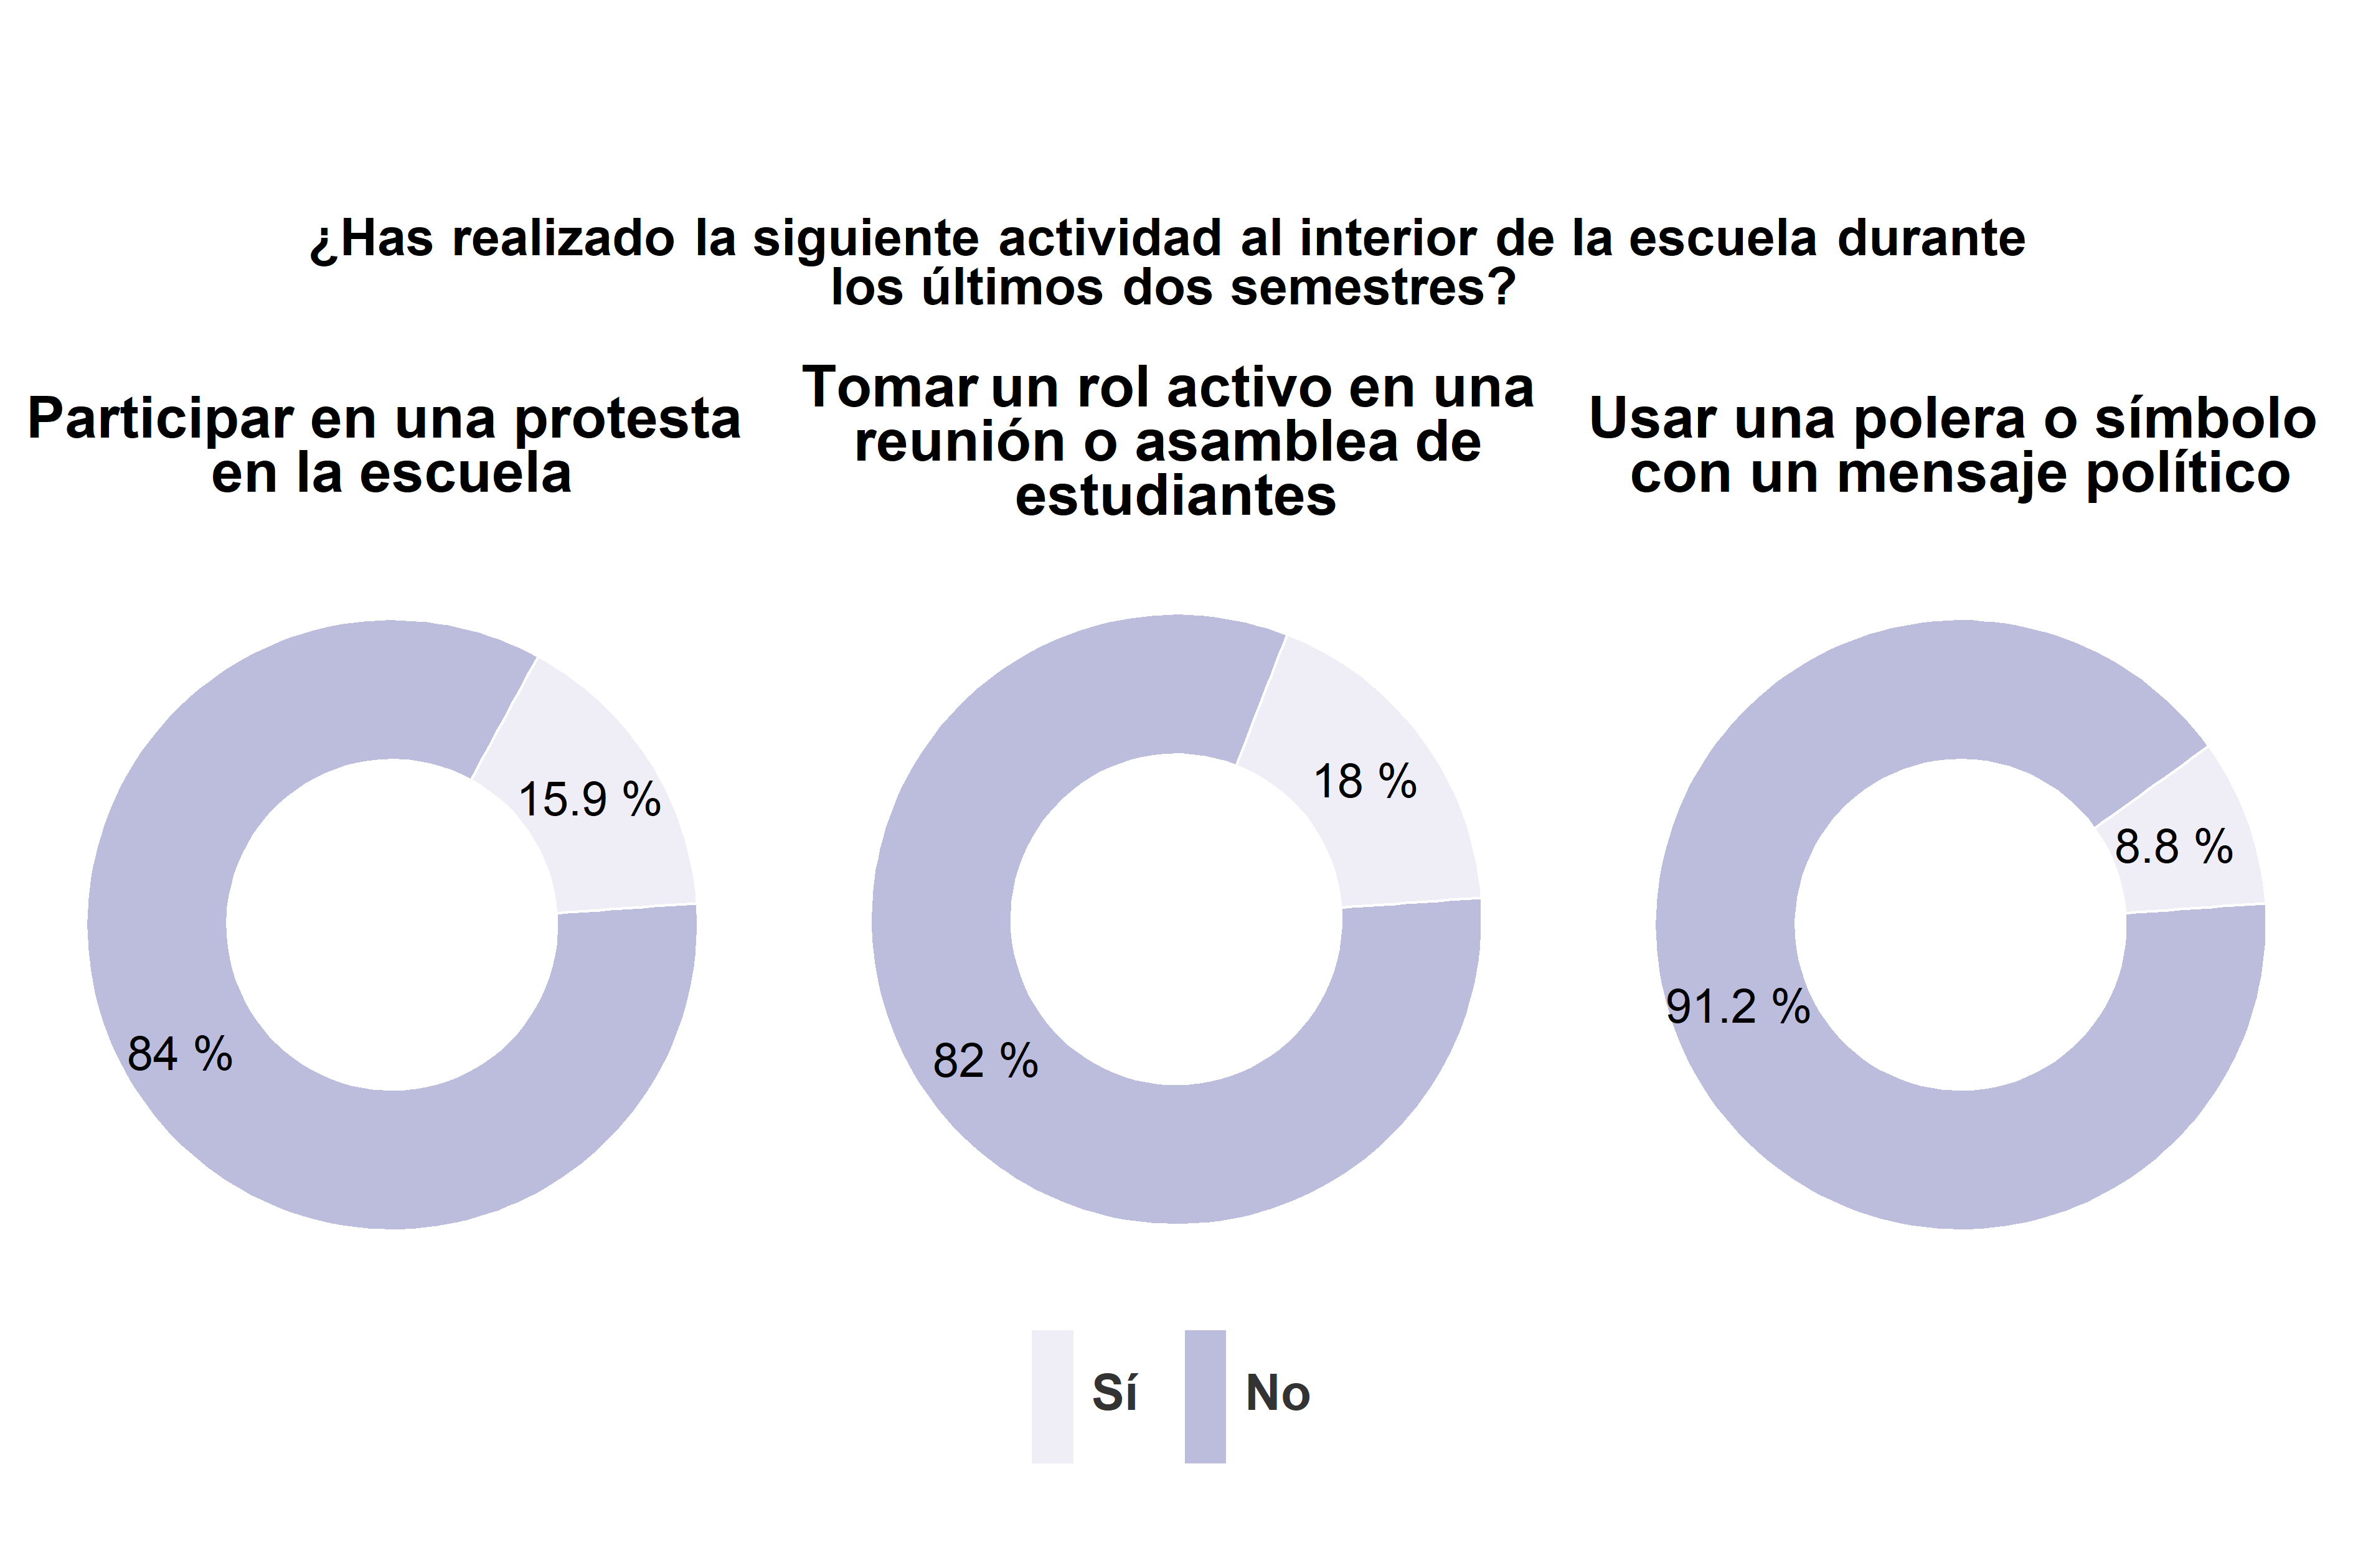
\includegraphics[width=0.8\linewidth,]{images/graph_partact_esc} 

}

\caption{Participación activista al interior de la escuela}\label{fig:unnamed-chunk-54}
\end{figure}

Son pocos los estudiantes que declaran haber realizado actividades de participación activista. La mayoría de los estudiantes declara que no ha participado en una protesta, tomado un rol activo en una reunión o asamblea de estudiantes, ni usado una polera o símbolo con un mensaje político al interior de la escuela durante los últimos dos semestres (un 83.3\%, un 84.7\% y un 91.5\%, respectivamente).

\begin{center}\rule{0.5\linewidth}{0.5pt}\end{center}

\begin{figure}[!ht]

{\centering \includegraphics[width=0.8\linewidth,]{images/graph_partact} 

}

\caption{Participación activista fuera de la escuela}\label{fig:unnamed-chunk-55}
\end{figure}

Como puede apreciarse la mayoría de los estudiantes no ha firmado una petición, ni ha participado en una marcha o una toma. Entre estas actividades, firmar una petición es aquella en la que más estudiantes ha participado (un 38.6\%).

\begin{center}\rule{0.5\linewidth}{0.5pt}\end{center}

\hypertarget{participaciuxf3n-comunitaria}{%
\section{Participación comunitaria}\label{participaciuxf3n-comunitaria}}

\begin{center}\rule{0.5\linewidth}{0.5pt}\end{center}

\begin{figure}[!ht]

{\centering \includegraphics[width=0.8\linewidth,]{images/graph_partcom_esc} 

}

\caption{Participación comunitaria al interior de la escuela}\label{fig:unnamed-chunk-56}
\end{figure}

Si bien la mayoría de los estudiantes no ha realizado trabajos voluntarios, colectas de dineros o bienes para ayudar a otros, ni actividades de ayuda a la comunidad al interior de la escuela durante los últimos dos semestres (un 62.1\%, un 52.5\% y un 61.9\%, respectivamente), el ámbito de la participación comunitaria al interior de la escuela es aquel en que una mayor proporción de estudiantes ha realizado actividades (en comparación con la participación formal y activista).

\begin{center}\rule{0.5\linewidth}{0.5pt}\end{center}

\begin{figure}[!ht]

{\centering \includegraphics[width=0.8\linewidth,]{images/graph_partcom} 

}

\caption{Participación comunitaria fuera de la escuela}\label{fig:unnamed-chunk-57}
\end{figure}

Pocos estudiantes han realizado actividades de participación comunitaria fuera de su escuela. La mayoría de los estudiantes no ha donado dinero por una buena causa, trabajado como voluntario para ayudar a personas de su comunidad, ni ha participado de una actividad social en la comunidad en que vive durante los últimos 12 meses (un 90.6\%, un 89.1\% y un 80.2\%, respectivamente).

\begin{center}\rule{0.5\linewidth}{0.5pt}\end{center}

  \bibliography{book.bib,packages.bib}

\end{document}
